\documentclass[8pt]{beamer} 

%% Math packages
%%
\usepackage{amsmath,amsthm,amssymb}
% Removes the "Too many math alphabets used in version normal" error.
\newcommand\hmmax{0}
\newcommand\bmmax{0}
\usepackage[new]{old-arrows}
\usepackage{cancel}
\usepackage{mathdots}
\usepackage{venndiagram}
\usepackage{mathrsfs}          % Math script font

% Graphics
%%
\graphicspath{{./}{figs/}}
\usepackage{graphicx}
\usepackage{tikz}
\usetikzlibrary{arrows}
\usetikzlibrary{decorations.markings}
\usetikzlibrary{decorations.pathreplacing}
\usetikzlibrary{patterns}
\usetikzlibrary{shapes.geometric}
\usetikzlibrary{matrix}
\usepackage{tikz-3dplot}
\usepackage{tkz-graph}
\usepackage{tikz-cd}

%% Colors (most are in colors.tex file)
%%
\usepackage{xcolor}
\usepackage{color}
\usepackage{visualalgebra}  %% Put this *after* the TikZ packages
\usepackage{visualalgebraslides}  %% Put this *after* "visualalgebra"

%% Page layout packages
%%
\usepackage{url}
\usepackage{multicol}
\usepackage{multirow}
\usepackage[numbers,square,sort&compress]{natbib}

%% Font and formatting packages
%%
\usepackage[english]{babel}    % Removing this causes compiler error
\usepackage{alltt}             % Like verbatim, but excludes \ and { }
\usepackage{enumerate}         % [shortlabels] option??
\usepackage{comment}
\usepackage{soul}              % strikeout text
\usepackage{bm}                % Bold math
\usepackage[T1]{fontenc}
\usepackage{relsize}

%% Fixes the \mathbf{} not working for fonts under 10pt
\usepackage{cmbright}
\fontencoding{OT1}\fontfamily{cmbr}\selectfont %to load ot1cmbr.fd
\DeclareFontShape{OT1}{cmbr}{bx}{n}{% change bx definition
<->cmbrbx10%
}{}
\normalfont

\makeatletter
\renewcommand*\env@matrix[1][\arraystretch]{%
  \edef\arraystretch{#1}%
  \hskip -\arraycolsep
  \let\@ifnextchar\new@ifnextchar
  \array{*\c@MaxMatrixCols c}}
\makeatother


%%=======================================================================

%% Beamer packages
%%
\mode<presentation>
{
  \usetheme{boadilla} 
  \useinnertheme{rectangles}
  \usecolortheme{dolphin}
}

\setbeamersize{text margin left=6mm}
\setbeamersize{text margin right=6mm}
\setbeamersize{sidebar width right=0mm}
\setbeamersize{sidebar width left=0mm}
\setbeamertemplate{navigation symbols}{}

\def\newblock{\hskip .11em plus .33em minus .07em}

% Other options: ball, circle, square 
\setbeamertemplate{enumerate items}[default]
%\setbeamercolor{enumerate subitem}{fg=red!80!black}
\def\opacity{0.5}
%setbeamercovered{transparent}
\setbeamercovered{invisible}

\newcommand{\Pause}{\pause}      %% Comment this out => lots more page breaks
% \newcommand{\Pause}{}

\AtBeginSection[]{
  \begin{frame}
  \vfill
  \centering
  \begin{beamercolorbox}[sep=8pt,center,shadow=true,rounded=true]{title}
    \usebeamerfont{title}\insertsectionhead\par%
  \end{beamercolorbox}
  \vfill
  \end{frame}
}


\begin{document}


%%====================================================================

\title[Subgroups!]{Subgroups!}

\author[\href{mailto:sbagley@westminsteru.edu}{S. Bagley}]
       {\href{mailto:sbagley@westminsteru.edu}{Spencer Bagley}}

\institute[Westminster] { 
  \normalsize With many thanks to Matthew Macauley, \\
  \url{http://www.math.clemson.edu/~macaule/}}

\date[10 Feb 2025]{10 Feb 2025}

\frame{\titlepage}

%%====================================================================

\begin{frame}{Goals for today:}
  \begin{enumerate}
    \item Define what subgroups are \Pause
    \item See some examples \Pause
    \item Figure out all the subgroups of all the groups of order 4 \Pause
    \item \ldots of order 6 \Pause
    \item \ldots of order 8
  \end{enumerate}
\end{frame}


%%====================================================================
\section{Definition time!}
%%====================================================================

\begin{frame}{Definition time!}
  Here is the definition of a subgroup. \smallskip

  \begin{block}{Definition}
    A \Alert{subgroup} of $G$ is a subset $H\subseteq G$ that
    is also a group. We denote this by $H\leq G$.
  \end{block} \Pause

  \smallskip
  Okay, but remind me what's the definition of a group? \Pause
  \smallskip

  \begin{block}{Definition}
    A \Alert{group} $(G, \star)$ is a set of elements together with a binary operation $\star$ satisfying the following properties: \Pause
    \begin{enumerate}
      \item The operation is associative. \Pause
      \item $G$ contains the identity element. \Pause
      \item Every element in $G$ has an inverse element. \Pause
      \item \Alert{$G$ is closed under the binary operation.}
    \end{enumerate}
  \end{block}\Pause

  \begin{alertblock}{Trivial subgroups}
    Every group $G$ has the following two boring subgroups: $G\leq G$, and $\{e\} \leq G$.
  \end{alertblock}\Pause

  \begin{block}{Definition}
    A \Alert{proper subgroup} $H < G$ is a subgroup that's not equal to the whole group.
  \end{block}
\end{frame}

%%====================================================================

\begin{frame}{Generating sets}
  We've previously looked at the \Alert{orbit} of an element: \Pause
  \begin{block}{Definition}
    The \Alert{orbit} of an element $g\in G$ is the \Balert{cyclic subgroup} that it generates,
    \[
    \<g\>=\big\{g^k\mid k\in\Z\big\},
    \]
    and its \Alert{order} is $|g|:=\big|\<g\>\big|$. \Pause

    In particular, if $|g| = n$ is finite, this is the set $\{g^0 = 1, g, g^2, \ldots, g^{n-1}\}$. \Pause
  \end{block}

  This is a subgroup: \Pause

  \begin{block}{Cyclic subgroups are subgroups}
    For any element $g\in G$, $\<g\> \leq G$.
  \end{block} \Pause

  But we need not restrain ourselves to generating by one element: \Pause

  \begin{block}{Definition}
    Let $S$ be a sub\Alert{set} of $G$. \Pause A \Alert{word} in $S$ is a finite product of finite powers of elements of $S$ or their inverses. \Pause

    \smallskip
    $\<S\> = \{\text{words in } S\}$ is a subgroup of $G$, and it's called the \Alert{subgroup generated by $S$}.
  \end{block} \Pause

  And in fact every subgroup looks like this.
\end{frame}


%%====================================================================

\begin{frame}{Example: $C_2 \leq D_3$} %\Pause
  
  Writing $C_2\leq D_3$ means \Balert{\emph{there is a copy of $C_2$ sitting
    inside of $D_3$ as a subgroup}}. \medskip\Pause

  \begin{exampleblock}{Question}
    How many ways can you find $C_2$ sitting inside of $D_3$?
    \begin{center}
    \begin{tikzpicture}[scale=0.5]
      \tikzstyle{r-out} = [draw, very thick, eRed,-stealth,bend right=43]
    \tikzstyle{r-in} = [draw, very thick, eRed,-stealth,bend left=38]
    %%
    \tikzstyle{every node}=[font=\small]
      \node (e) at (0:2) [v] {$1$};
      \node (r) at (120:2) [v] {$r$};
      \node (r2) at (240:2) [v] {$r^2$};
      \node (f) at (0:1) [v] {$f$};
      \node (r2f) at (240:1) [v] {$r^2\!f$};
      \node (rf) at (120:1) [v] {$rf$};
      \draw [r-out] (e) to (r);
      \draw [r-out] (r) to (r2);
      \draw [r-out] (r2) to (e);
      \draw [r-in] (f) to (r2f);
      \draw [r-in] (r2f) to (rf);
      \draw [r-in] (rf) to (f);
      \draw [bb] (e) to (f);
      \draw [bb] (r) to (rf);
      \draw [bb] (r2) to (r2f);
    \end{tikzpicture}\end{center}
  \end{exampleblock}\Pause
  
  \begin{alertblock}{Remark}
    It's more precise to express a subgroup by its generator(s). \Pause

    \hfill $C_2 \cong \<f\> < D_3$ \hfill $C_2 \cong \<rf\> < D_3$ \hfill $C_2 \cong \<r^2f\> < D_3$ \hfill \phantom{.}
  \end{alertblock}

  \begin{exampleblock}{Question}
    How about $C_3 \leq D_3$? \Pause \Alert{There's only one!}
    
  \end{exampleblock}
  
\end{frame}

%%====================================================================
\section{Groups of order $4$}
%%====================================================================

\begin{frame}{The two groups of order $4$} 
  
  Let's start by considering the subgroups of the two groups of order $4$.
  
  %% Cayley graphs of C_4 and V_4
  \[
  \begin{tikzpicture}[scale=.8]
    %%
    \tikzstyle{every node}=[font=\small]
    %%
    \begin{scope}[shift={(0,0)},scale=.95]
      \tikzstyle{every node}=[font=\small]
      \node (j) at (-1,-1) [v] {$v$};
      \node (1) at (-1,1) [v] {$e$};
      \node (k) at (1,-1) [v] {$r$};
      \node (i) at (1,1) [v] {$h$};
      \draw [rr] (1) to (i);
      \draw [rr] (j) to (k);
      \draw [bb] (1) to (j);
      \draw [bb] (i) to (k);
      \node at (0,0) {\normalsize $V_4\!=\!\<h,v\>$};
    \end{scope}
    %%
    \begin{scope}[shift={(5,0)}]
      \node (e) at (0:1) [v] {$1$};
      \node (r3) at (270:1) [v] {$r^3$};
      \node (r2) at (180:1) [v] {$r^2$};
      \node (r) at (90:1) [v] {$r$};
      \draw [r] (e) to [bend right=25] (r);
      \draw [r] (r) to [bend right=25] (r2);
      \draw [r] (r2) to [bend right=25] (r3);
      \draw [r] (r3) to [bend right=25] (e);
      \node at (0,0) {$C_4\!=\!\<r\>$};
    \end{scope}
  \end{tikzpicture}
  \]\Pause
  \vspace{-5mm}
  \begin{itemize}
  \item Proper subgroups of $V_4$: $\<h\>=\{e,h\}$,\;
    $\<v\>=\{e,v\}$,\; $\<r\>=\{e,r\}$,\; $\<e\>=\{e\}$. \smallskip\Pause
  \item Subgroups of $C_4$: $\<r\>=\{1,r,r^2,r^3\}=\<r^3\>$,\;
    $\<r^2\>=\{1,r^2\}$,\; $\<1\>=\{1\}$.
  \end{itemize}
  
  \medskip\Pause
  
  It is illustrative to arrange these in a \Balert{subgroup lattice}: 
  
  %% Subgroup lattices of V_4 and C_4
  \[
  \begin{tikzpicture}[shorten >= -2pt, shorten <= -2pt,scale=1.25]
    %%
    \tikzstyle{every node}=[font=\normalsize]
    %%
    \begin{scope}[shift={(0,0)}]
      \node (V4) at (0,2) {\hspace{-6mm}$V_4\!=\!\<h,v\>$};
      \node (h) at (-.75,1) {$\<h\>$};
      \node (r) at (0,1) {$\<r\>$};
      \node (v) at (.75,1) {$\<v\>$};
      \node (e) at (0,0) {$\<e\>$};
      \draw (V4)--(h); 
      \draw (V4)--(r); 
      \draw (V4)--(v);
      \draw (h)--(e);
      \draw (r)--(e); 
      \draw (v)--(e); 
    \end{scope}
    %%
    \begin{scope}[shift={(3,0)}]
      \node (C4) at (0,2) {\hspace{-6mm}$C_4\!=\!\<r\>$};
      \node (r2) at (0,1) {$\<r^2\>$};
      \node (1) at (0,0) {$\<1\>$};
      \draw (C4)--(r2); %node[midway, right]{$2$};
      \draw (r2)--(1); %node[midway, right]{$3$};
    \end{scope}
    %%
    \begin{scope}[shift={(7.5,0)}]
      \node [anchor=east] at (0,2) {\textbf{Order}:\quad $4$};
      \node [anchor=east] at (0,1) {$2$};
      \node [anchor=east] at (0,0) {$1$};
    \end{scope}
  \end{tikzpicture}
  \]
  
\end{frame}

%%====================================================================
\section{Groups of order $6$}
%%====================================================================

\begin{frame}{Subgroups of $\Z_6$}

  What subgroups can you find in $\Z_6$? I've drawn the Cayley diagram two different ways.

  \[
  \begin{tikzpicture}
    %%
    \tikzstyle{r-bend} = [draw,very thick, eRed,-stealth,bend right=15]
    \tikzstyle{g-out} = [draw,very thick, eGreen,-stealth,bend right=42]
    \tikzstyle{g-in} = [draw,very thick, eGreen,-stealth,bend right=35]
    %%
    \begin{scope}[shift={(0,0)}]
      \tikzstyle{every node}=[font=\small]
      \node (0) at (0:2) [v] {$0$};
      \node (1) at (60:2) [v] {$1$};
      \node (2) at (120:2) [v] {$2$};
      \node (3) at (180:2) [v] {$3$};
      \node (4) at (240:2) [v] {$4$};
      \node (5) at (300:2) [v] {$5$};
      \path[r-bend] (0) to (1);
      \path[r-bend] (1) to (2);
      \path[r-bend] (2) to (3);
      \path[r-bend] (3) to (4);
      \path[r-bend] (4) to (5);
      \path[r-bend] (5) to (0);
      \node at (0,0) {\normalsize $\<1\>$};
      \node at (270:2.5) {Hello I am secretly also the cycle graph};
    \end{scope}
    %%
    \begin{scope}[shift={(6,0)},scale=1.15]
      \tikzstyle{every node}=[font=\small]
      \node (0) at (0:2) [v] {$0$};
      \node (2) at (120:2) [v] {$2$};
      \node (4) at (240:2) [v] {$4$};
      \node (3) at (0:1) [v] {$3$};
      \node (5) at (120:1) [v] {$5$};
      \node (1) at (240:1) [v] {$1$};
      \draw [g-in] (3) to (5);
      \draw [g-in] (5) to (1);
      \draw [g-in] (1) to (3);
      \draw [g-out] (0) to (2);
      \draw [g-out] (2) to (4);
      \draw [g-out] (4) to (0);
      \draw [bb] (3) to (0);
      \draw [bb] (5) to (2);
      \draw [bb] (1) to (4);
      \node at (0,0) {\normalsize $\<2,3\>$};
    \end{scope}
  \end{tikzpicture}
  \]
  
\end{frame}

%%====================================================================

\begin{frame}{Subgroups of $D_3$}
  
  Let's figure out all the subgroups of $D_3$.

  %% Cayley graph, cycle graph, and subgroup lattice of D_3
  \[
  \begin{tikzpicture}[scale=.6]
    %%
    \tikzstyle{r-out} = [draw, very thick, eRed,-stealth,bend right=43]
    \tikzstyle{r-in} = [draw, very thick, eRed,-stealth,bend left=38]
    %%
    \begin{scope}[shift={(-.5,0)},scale=1.05]
      \tikzstyle{every node}=[font=\small]
      \node (e) at (0:2) [v] {$1$};
      \node (r) at (120:2) [v] {$r$};
      \node (r2) at (240:2) [v] {$r^2$};
      \node (f) at (0:1) [v] {$f$};
      \node (r2f) at (240:1) [v] {$r^2\!f$};
      \node (rf) at (120:1) [v] {$rf$};
      \draw [r-out] (e) to (r);
      \draw [r-out] (r) to (r2);
      \draw [r-out] (r2) to (e);
      \draw [r-in] (f) to (r2f);
      \draw [r-in] (r2f) to (rf);
      \draw [r-in] (rf) to (f);
      \draw [bb] (e) to (f);
      \draw [bb] (r) to (rf);
      \draw [bb] (r2) to (r2f);
    \end{scope}
    %%
    \begin{scope}[shift={(5,-.8)},scale=.8]
      \tikzstyle{every node}=[font=\small]
      \node (1) at (90:2) [v-r] {$1$};
      \node (r) at (210:2) [v-r] {$r$};
      \node (r2) at (330:2) [v-r] {$r^2$};
      \node (f) at (-1.5,4) [v-p] {$f$};
      \node (rf) at (0,4) [v-p] {$rf$};
      \node (r2f) at (1.5,4) [v-p] {$r^2\!f$};           
      \draw [cy2] (1) to [bend right] (r);
      \draw [cy2] (r) to [bend right] (r2);
      \draw [cy2] (r2) to [bend right] (1);
      \draw [cy2] (1) to (f);
      \draw [cy2] (1) to (rf);
      \draw [cy2] (1) to (r2f);
    \end{scope}
  \end{tikzpicture}
  \] \Pause

  Here are the \Balert{non-trivial proper subgroups} of $D_3$:
  \[
  \<r\>=\{1,r,r^2\}=\<r^2\>,\quad \<f\>=\{1,f\},\quad
  \<rf\>=\{1,rf\},\quad\<r^2f\>=\{1,r^2f\}\Pause,\Alert{\quad\<1\>=\{1\}}.
  \] \Pause
  
  Observations: 
  \begin{itemize}
    \item The cycle graph helps us spot cyclic subgroups. \Pause
    \item For small groups like $D_3$, the cyclic subgroups may be the \Alert{only} proper subgroups. \Pause
    \item There might, however, be more complicated things that are harder to clock.
  \end{itemize}

\end{frame}

%%====================================================================
\section{Groups of order $8$}
%%====================================================================

\begin{frame}{Subgroups of $D_4$}

  See if you can figure out all the subgroups of $D_4$.
  
  %% Cayley graph and subgroup lattice of D_4
  \[
  \begin{tikzpicture}[scale=.6]
    %%
    \tikzstyle{r-out} = [draw, very thick, eRed,-stealth,bend right=33]
    \tikzstyle{r-in} = [draw, very thick, eRed,-stealth,bend left=25]
    %% Square with actions highlighted
    \begin{scope}[shift={(-7,-0.5)}, scale=1.2]
      \draw [dashed,very thick,eBlue] (.5,-1) to (.5,2);
      \draw [dashed,ePurple,thick] (-1,.5) to (2,.5);
      \draw [dashed,eOrange,thick] (-.75,1.75) to (1.75,-.75);
      \draw [dashed,eGreen,thick] (-.75,-.75) to (1.75,1.75);
      \path[fill=actRed] (0,.5) rectangle ++(.5,.5); 
      \path[fill=actYellow] (.5,.5) rectangle ++(.5,.5);
      \path[fill=actGreen] (0,0) rectangle ++(.5,.5);
      \path[fill=actBlue] (.5,0) rectangle ++(.5,.5);
      \draw (.25,.75) node{$\mathbf{1}$};
      \draw (.75,.75) node{$\mathbf{2}$};
      \draw (.25,.25) node{$\mathbf{4}$};
      \draw (.75,.25) node{$\mathbf{3}$};
      \draw (0,0) rectangle (1,1);
      \draw[-stealth',eRed] (2,0) to[very thick,bend right=60] (2,.8);
      \node[xRed] at (2.5,.5) {$r$};
      \node[xBlue] at (.3,2.1) {$f$};
    \end{scope}
    %% Cayley graph
    \begin{scope}[shift={(0,0)},scale=1]
      \tikzstyle{every node}=[font=\small]
      \node (e) at (0:2) [v] {$1$};
      \node (r) at (90:2) [v] {$r$};
      \node (r2) at (180:2) [v] {$r^2$};
      \node (r3) at (270:2) [v] {$r^3$};
      \node (f) at (0:1) [v] {$f$};
      \node (r3f) at (270:1) [v] {$r^3\!f$};
      \node (r2f) at (180:1) [v] {$r^2\!f$};
      \node (rf) at (90:1) [v] {$rf$};
      \draw [r-out] (e) to (r);
      \draw [r-out] (r) to (r2);
      \draw [r-out] (r2) to (r3);
      \draw [r-out] (r3) to (e);
      \draw [r-in] (f) to (r3f);
      \draw [r-in] (r3f) to (r2f);
      \draw [r-in] (r2f) to (rf);
      \draw [r-in] (rf) to (f);
      \draw [bb] (e) to (f);
      \draw [bb] (r) to (rf);
      \draw [bb] (r2) to (r2f);
      \draw [bb] (r3) to (r3f);
    \end{scope}
    %% Cycle graph
    \begin{scope}[shift={(6,-.75)},scale=.8]
      \tikzstyle{every node}=[font=\small]
      \node (1) at (90:2) [v-gr] {$1$};
      \node (r) at (180:2) [v-r] {$r$};
      \node (r2) at (270:2) [v-p] {$r^2$};
      \node (r3) at (0:2) [v-r] {$r^3$};
      \node (f) at (-2.25,4) [v-b] {$f$};
      \node (r2f) at (-.75,4) [v-b] {$r^2f$};
      \node (rf) at (.75,4) [v-g] {$rf$};
      \node (r3f) at (2.25,4) [v-g] {$r^3f$};
      \draw [cy2] (1) to [bend right] (r);
      \draw [cy2] (r) to [bend right] (r2);
      \draw [cy2] (r2) to [bend right] (r3);
      \draw [cy2] (r3) to [bend right] (1);
      \draw [cy2] (1) to (f);
      \draw [cy2] (1) to (rf);
      \draw [cy2] (1) to (r2f);
      \draw [cy2] (1) to (r3f);
      \node at (0,0) {\normalsize $D_4$};
    \end{scope}
  \end{tikzpicture}
  \]\Pause

  What do you think is a reasonable way to, like, arrange them?
  
\end{frame}

%%====================================================================
\subsection{Lattices}
%%====================================================================

\begin{frame}{Lattices} %\Pause
  
  A \Alert{lattice} is a \Balert{partially ordered set} such that
  every pair of elements $x,y$ has a \Alert{unique}: \vspace{-2mm} \Pause
  \begin{multicols}{2}
    \begin{itemize}
    \item \Galert{join}, or \Alert{sup}, or \Balert{least upper bound} \\$x\!\Or\!y$ \Pause
    \item \Galert{meet}, or \Alert{inf}, or \Balert{greatest lower bound}\\ $x\!\And\!y$.\Pause
    \end{itemize}
  \end{multicols}
  Examples you may have seen previously are \Balert{subset lattices} and
  \Balert{divisor lattices}.
  %%
  %% Boolean lattice, and divisor lattice of 24
  \[
  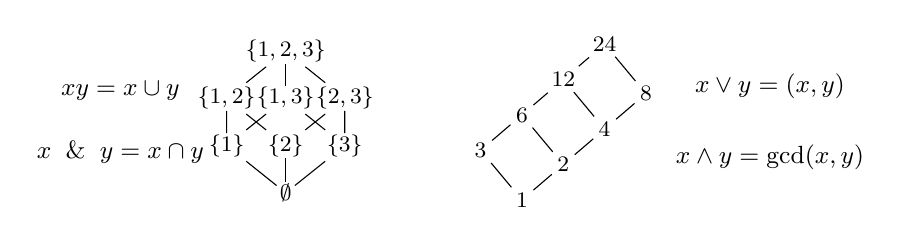
\begin{tikzpicture}[shorten >= -3pt, shorten <= -3pt, scale=1]
    %%
    \tikzstyle{every node}=[font=\footnotesize]
    %%
    \begin{scope}[shift={(0,0)},scale=.6]
      \node (123) at (0,3) {$\{1,2,3\}$};
      \node (12) at (-1.25,2) {$\{1,2\}$};
      \node (13) at (0,2) {$\{1,3\}$};
      \node (23) at (1.25,2) {$\{2,3\}$};
      \node (1) at (-1.25,1) {$\{1\}$};
      \node (2) at (0,1) {$\{2\}$};
      \node (3) at (1.25,1) {$\{3\}$};
      \node (null) at (0,0) {$\emptyset$};
      \draw (123) -- (12); \draw (123) -- (13); \draw (123) -- (23);
      \draw (12) -- (1); \draw (12) -- (2);
      \draw (13) -- (1); \draw (13) -- (3);
      \draw (23) -- (2); \draw (23) -- (3);
      \draw (1) to (null); \draw (2) to (null); \draw (3) to (null);
      \node at (-3.5,2.15) {\small $x\Or y=x\cup y$};
      \node at (-3.5,.85) {\small $x\And y=x\cap y$};
    \end{scope}
    %%
    \begin{scope}[shift={(3,0)},scale=.3,shorten >= -2pt, shorten <= -2pt]
      \node(G) at (3.5,6+.3) {$24$};
      \node(r2-s) at (1.75,4.5+.3) {$12$};
      \node(r) at (5.25,4.5-.3) {$8$};
      \node(r4-s) at (0,3+.3) {$6$};
      \node(r2) at (3.5,3-.3) {$4$};
      \node(s) at (-1.75,1.5+.3) {$3$};
      \node(r4) at (1.75,1.5-.3) {$2$};
      \node(1) at (0,0-.3) {$1$};
      \draw (1) to (s);
      \draw (1) to (r4);
      \draw (s) to (r4-s);
      \draw (r4) to (r4-s);
      \draw (r4) to (r2);
      \draw (r4-s) to (r2-s);
      \draw (r2) to (r2-s);
      \draw (r2) to (r);
      \draw (r2-s) to (G);
      \draw (r) to (G);
      \node at (10.5,4.5) {\small $x\vee y=\lcm(x,y)$};
      \node at (10.5,1.5) {\small $x\wedge y=\gcd(x,y)$};
    \end{scope}
  \end{tikzpicture}
  \]
  
  This seems like a good way to organize subgroups, because: \Pause

  \begin{block}{Theorem}
    If $H \leq G$ and $K \leq G$ are two subgroups, then $H\cap K$ is a subgroup. \Pause

    (Indeed, it's the largest subgroup that's contained in both $H$ and $K$.)
  \end{block} \Pause

  \begin{block}{Theorem}
    $\<H, K\>$ is the smallest subgroup containing both $H$ and $K$. \Pause

    (Note that $H \cup K$ is not in general a subgroup. Why not?)
  \end{block}
\end{frame}


\begin{frame}{Subgroup lattices}

  %% Subgroup lattice of H, K, H\cap K, and <H,K>
  \[
  \begin{tikzpicture}[shorten >= -2pt, shorten <= -2pt]
    %%
    \tikzstyle{every node}=[font=\normalsize]
    %%
    \begin{scope}[shift={(0,0)}]
      \node (HcupK) at (0,2) {$\<H,K\>$};
      \node (H) at (-.75,1.1) {$H$}; \node (K) at (.75,.9) {$K$};
      \node (HcapK) at (0,0) {$H\cap K$};
      \draw (HcupK) -- (H); \draw (HcupK) -- (K);
      \draw (H) -- (HcapK); \draw (K) -- (HcapK);
      \node at (6,2)
        { $H\Or K$: ``\emph{smallest subgroup above both $H$ and $K$}''};
      \node at (6,0)
        { $H\And K$: ``\emph{largest subgroup below both $H$ and $K$}''};
    \end{scope}
  \end{tikzpicture}
  \] \Pause
  Examples:
  \[
  \begin{tikzpicture}
    \begin{scope}[shift={(0,-3.3)},shorten >= -2pt, shorten <= -2pt,scale=.9]
      \node(G) at (0,6) {\hspace{-7mm}$\Z_6\!=\!\<1\>$};
      \node(2) at (-1.5,4.5) {$\<2\>$};
      \node(3) at (1.5,3.3) {$\<3\>$};
      \node(0) at (0,1.5) {$\<0\>$};
      \draw (G) to (2); \draw (G) to (3); \draw (2) to (0); \draw (3) to (0);
    \end{scope} \Pause
    \begin{scope}[shift={(5,-3.5)},shorten >= -2pt, shorten <= -2pt,scale=.95]
      \node(G) at (0,6) {\hspace{-7mm}$D_3\!=\!\<r,f\>$};
      \node(r) at (-1.75,4.5) {$\<r\>$};
      \node(e) at (0,1.5) {$\<1\>$};
      \node(f) at (.2,3.3) {$\<f\>$};
      \node(rf) at (1.55,3.3) {$\<rf\>$};
      \node(r2f) at (3,3.3) {$\<r^2\!f\>$};
      \draw(G)--(r); 
      \draw(G)--(f); 
      \draw(G)--(rf); 
      \draw(G)--(r2f); 
      \draw(r)--(e); 
      \draw(f)--(e); 
      \draw(rf)--(e); 
      \draw(r2f)--(e);
      \node [anchor=east] at (4.5,6) {\textbf{Order}:\;\; 6};
      \node [anchor=east] at (4.5,4.5) {3};
      \node [anchor=east] at (4.5,3.3) {2};
      \node [anchor=east] at (4.5,1.5) {1};
   \end{scope}
  \end{tikzpicture}
  \]
  
\end{frame}

%%====================================================================

\begin{frame}{The subgroup lattice of $D_4$}
  
  \begin{columns}
    
    \begin{column}{.725\textwidth}
      The subgroups of $D_4$ are: \smallskip\Pause 
      \begin{itemize}
      \item The entire group $D_4$, and the trivial group
        $\<1\>$ \smallskip\Pause
      \item 4 subgroups generated by reflections: 
        $\<f\>$, $\<rf\>$, $\<r^2f\>$, $\<r^3f\>$. \smallskip\Pause 
      \item 1 subgroup generated by a $180^\circ$
        rotation, $\<r^2\>\cong C_2$ \smallskip\Pause 
      \item 1 subgroup generated by a $90^\circ$
        rotation, $\<r\>\cong C_4$ \smallskip\Pause 
      \item 2 subgroups isomorphic to $V_4$: $\<r^2,f\>$,
        $\<r^2,rf\>$.
      \end{itemize}
    \end{column}
    
    \begin{column}{.25\textwidth}
      %%
      %% Square with the four axis of reflection shown.
      \[
      \begin{tikzpicture}
        \begin{scope}[scale=.8]
          \draw [dashed,very thick,eBlue] (.5,-1) to (.5,2);
          \draw [dashed,ePurple,thick] (-1,.5) to (2,.5);
          \draw [dashed,eOrange,thick] (-.75,1.75) to (1.75,-.75);
          \draw [dashed,eGreen,thick] (-.75,-.75) to (1.75,1.75);
          \path[fill=actRed] (0,.5) rectangle ++(.5,.5); 
          \path[fill=actYellow] (.5,.5) rectangle ++(.5,.5);
          \path[fill=actGreen] (0,0) rectangle ++(.5,.5);
          \path[fill=actBlue] (.5,0) rectangle ++(.5,.5);
          \draw (.25,.75) node{$\mathbf{1}$};
          \draw (.75,.75) node{$\mathbf{2}$};
          \draw (.25,.25) node{$\mathbf{4}$};
          \draw (.75,.25) node{$\mathbf{3}$};
          \draw (0,0) rectangle (1,1);
          \draw[-stealth',eRed] (2,0) to[very thick,bend right=60] (2,.8);
          \node[xRed] at (2.5,.5) {$r$};
          \node[xBlue] at (.3,2.1) {$f$};
        \end{scope}
      \end{tikzpicture}
      \]
    \end{column}
    
  \end{columns}
  
  \bigskip\Pause
  
  %% Cayley graph and subgroup lattice of D_4
  \[
  \begin{tikzpicture}[scale=.68]
    %%
    \tikzstyle{r-out} = [draw, very thick, eRed,-stealth,bend right=33]
    \tikzstyle{r-in} = [draw, very thick, eRed,-stealth,bend left=25]
    %%
    \begin{scope}[shift={(0,0)},scale=1]
      \tikzstyle{every node}=[font=\small]
      \node (e) at (0:2) [v] {$1$};
      \node (r) at (90:2) [v] {$r$};
      \node (r2) at (180:2) [v] {$r^2$};
      \node (r3) at (270:2) [v] {$r^3$};
      \node (f) at (0:1) [v] {$f$};
      \node (r3f) at (270:1) [v] {$r^3\!f$};
      \node (r2f) at (180:1) [v] {$r^2\!f$};
      \node (rf) at (90:1) [v] {$rf$};
      \draw [r-out] (e) to (r);
      \draw [r-out] (r) to (r2);
      \draw [r-out] (r2) to (r3);
      \draw [r-out] (r3) to (e);
      \draw [r-in] (f) to (r3f);
      \draw [r-in] (r3f) to (r2f);
      \draw [r-in] (r2f) to (rf);
      \draw [r-in] (rf) to (f);
      \draw [bb] (e) to (f);
      \draw [bb] (r) to (rf);
      \draw [bb] (r2) to (r2f);
      \draw [bb] (r3) to (r3f);
    \end{scope}
    %%
    \begin{scope}[shift={(5,-.75)},scale=.8]
      \tikzstyle{every node}=[font=\small]
      \node (1) at (90:2) [v-gr] {$1$};
      \node (r) at (180:2) [v-r] {$r$};
      \node (r2) at (270:2) [v-p] {$r^2$};
      \node (r3) at (0:2) [v-r] {$r^3$};
      \node (f) at (-2.25,4) [v-b] {$f$};
      \node (r2f) at (-.75,4) [v-b] {$r^2f$};
      \node (rf) at (.75,4) [v-g] {$rf$};
      \node (r3f) at (2.25,4) [v-g] {$r^3f$};
      \draw [cy2] (1) to [bend right] (r);
      \draw [cy2] (r) to [bend right] (r2);
      \draw [cy2] (r2) to [bend right] (r3);
      \draw [cy2] (r3) to [bend right] (1);
      \draw [cy2] (1) to (f);
      \draw [cy2] (1) to (rf);
      \draw [cy2] (1) to (r2f);
      \draw [cy2] (1) to (r3f);
      \node at (0,0) {\normalsize $D_4$};
    \end{scope} \Pause
    %%
    \begin{scope}[shift={(11.25,-3.5)},scale=1.35,shorten >= -2pt,
        shorten <= -2pt]
      \node (D4) at (0,4) {$D_4$};
      \node (r2-f) at (-1.25,3) {$\<r^2,f\>$};
      \node (r) at (0,3) {$\<r\>$};
      \node (r2-rf) at (1.25,3) {$\<r^2,rf\>$};
      \node (f) at (-2.5,2) {$\<f\>$};
      \node (r2f) at (-1.25,2) {$\<r^2f\>$};
      \node (r2) at (0,2) {$\<r^2\>$};
      \node (r3f) at (1.25,2) {$\<r^3f\>$};
      \node (rf) at (2.5,2) {$\<rf\>$};
      \node (1) at (0,1) {$\<1\>$};
      %%
      \draw (D4) to (r2-f); \draw (D4) to (r); \draw (D4) to (r2-rf);
      \draw (r2-f) to (f); \draw (r2-f) to (r2f); \draw (r2-f) to (r2);
      \draw (r2-rf) to (rf); \draw (r2-rf) to (r3f); \draw (r2-rf) to (r2);
      \draw (r2) to (r);
      \draw (r2) to (1);
      \draw (f) to (1);
      \draw (r2f) to (1); \draw (r3f) to (1); \draw (rf) to (1);
    \end{scope}
  \end{tikzpicture}
  \]
  
\end{frame}

%%====================================================================

\begin{frame}{The subgroup lattice of $D_4$} %\Pause
  
  \vspace{-3mm}  
  
  %% Subgroup lattice of D_4 with cycle graphs for nodes
  \[
  \scalebox{.75}{
    \begin{tikzpicture}[scale=.75]
      %%
      \tikzstyle{v-r}=[circle,draw,fill=vRed,inner sep=0pt,minimum size=1.7mm]
      \tikzstyle{v-g}=[circle,draw,fill=vGreen,inner sep=0pt,minimum size=1.7mm]
      \tikzstyle{v-b}=[circle,draw,fill=vBlue,inner sep=0pt,minimum size=1.7mm]
      \tikzstyle{v-p}=[circle,draw,fill=vPurple,inner sep=0pt,minimum size=1.7mm]
      \tikzstyle{v-w}=[circle,draw,fill=white,inner sep=0pt,minimum size=1.7mm]
      \tikzstyle{v-gr}=[circle,draw,fill=midgray,inner sep=0pt,minimum size=1.7mm]
      \tikzstyle{lat} = [draw,very thick,faded]
      %%
      \begin{scope}[shift={(0,12)},scale=.4]
        \node (1) at (90:1.6) [v-gr] {};
        \node (r) at (180:1.6) [v-r] {};
        \node (r2) at (270:1.6) [v-p] {};
        \node (r3) at (0:1.6) [v-r] {};
        \node (f) at (-1.8,3) [v-b] {};
        \node (r2f) at (-.6,3) [v-b] {};
        \node (rf) at (.6,3) [v-g] {};
        \node (r3f) at (1.8,3) [v-g] {};
        \draw [cy2] (1) to [bend right=30] (r);
        \draw [cy2] (r) to [bend right=30] (r2);
        \draw [cy2] (r2) to [bend right=30] (r3);
        \draw [cy2] (r3) to [bend right=30] (1);
        \draw [cy2] (1) to (f);
        \draw [cy2] (1) to (rf);
        \draw [cy2] (1) to (r2f);
        \draw [cy2] (1) to (r3f);
        \node at (0,0) {$D_4$};
        \node (D4-bot) at (0,-2) {};
      \end{scope}
      %%  
      \begin{scope}[shift={(-4,8)},scale=.4]
        \node (1) at (90:1.6) [v-gr] {};
        \node (r) at (180:1.6) [v-w] {};
        \node (r2) at (270:1.6) [v-p] {};
        \node (r3) at (0:1.6) [v-w] {};
        \node (f) at (-1.8,3) [v-b] {};
        \node (r2f) at (-.6,3) [v-b] {};
        \node (rf) at (.6,3) [v-w] {};
        \node (r3f) at (1.8,3) [v-w] {};
        \draw [cy2] (1) to [bend right=30] (r);
        \draw [cy2] (r) to [bend right=30] (r2);
        \draw [cy2] (r2) to [bend right=30] (r3);
        \draw [cy2] (r3) to [bend right=30] (1);
        \draw [cy2] (1) to (f);
        \draw [cy2] (1) to (rf);
        \draw [cy2] (1) to (r2f);
        \draw [cy2] (1) to (r3f);
        \node at (0,0) {\small $\<r^2\!,f\>$};
        \node (r2-f-top) at (0,3.5) {};
        \node (r2-f-bot) at (0,-2) {};
      \end{scope}
      %%
      \begin{scope}[shift={(0,8)},scale=.4]
        \node (1) at (90:1.6) [v-gr] {};
        \node (r) at (180:1.6) [v-r] {};
        \node (r2) at (270:1.6) [v-p] {};
        \node (r3) at (0:1.6) [v-r] {};
        \node (f) at (-1.8,3) [v-w] {};
        \node (r2f) at (-.6,3) [v-w] {};
        \node (rf) at (.6,3) [v-w] {};
        \node (r3f) at (1.8,3) [v-w] {};
        \draw [cy2] (1) to [bend right=30] (r);
        \draw [cy2] (r) to [bend right=30] (r2);
        \draw [cy2] (r2) to [bend right=30] (r3);
        \draw [cy2] (r3) to [bend right=30] (1);
        \draw [cy2] (1) to (f);
        \draw [cy2] (1) to (rf);
        \draw [cy2] (1) to (r2f);
        \draw [cy2] (1) to (r3f);
        \node at (0,0) {$\<r\>$};
        \node (r-top) at (0,3.5) {};
        \node (r-bot) at (0,-2) {};
      \end{scope}
      %%
      \begin{scope}[shift={(4,8)},scale=.4]
        \node (1) at (90:1.6) [v-gr] {};
        \node (r) at (180:1.6) [v-w] {};
        \node (r2) at (270:1.6) [v-p] {};
        \node (r3) at (0:1.6) [v-w] {};
        \node (f) at (-1.8,3) [v-w] {};
        \node (r2f) at (-.6,3) [v-w] {};
        \node (rf) at (.6,3) [v-g] {};
        \node (r3f) at (1.8,3) [v-g] {};
        \draw [cy2] (1) to [bend right=30] (r);
        \draw [cy2] (r) to [bend right=30] (r2);
        \draw [cy2] (r2) to [bend right=30] (r3);
        \draw [cy2] (r3) to [bend right=30] (1);
        \draw [cy2] (1) to (f);
        \draw [cy2] (1) to (rf);
        \draw [cy2] (1) to (r2f);
        \draw [cy2] (1) to (r3f);
        \node at (0,0) {\small $\<r^2\!,rf\>$};
        \node (r2-rf-top) at (0,3.5) {};
        \node (r2-rf-bot) at (0,-2) {};
      \end{scope}
      %%
      \begin{scope}[shift={(-8,4)},scale=.4]
        \node (1) at (90:1.6) [v-gr] {};
        \node (r) at (180:1.6) [v-w] {};
        \node (r2) at (270:1.6) [v-w] {};
        \node (r3) at (0:1.6) [v-w] {};
        \node (f) at (-1.8,3) [v-b] {};
        \node (r2f) at (-.6,3) [v-w] {};
        \node (rf) at (.6,3) [v-w] {};
        \node (r3f) at (1.8,3) [v-w] {};
        \draw [cy2] (1) to [bend right=30] (r);
        \draw [cy2] (r) to [bend right=30] (r2);
        \draw [cy2] (r2) to [bend right=30] (r3);
        \draw [cy2] (r3) to [bend right=30] (1);
        \draw [cy2] (1) to (f);
        \draw [cy2] (1) to (rf);
        \draw [cy2] (1) to (r2f);
        \draw [cy2] (1) to (r3f);
        \node at (0,0) {$\<f\>$};
        \node (f-top) at (0,3.5) {};
        \node (f-bot) at (0,-2) {};
      \end{scope}
      %%
      \begin{scope}[shift={(-4,4)},scale=.4]
        \node (1) at (90:1.6) [v-gr] {};
        \node (r) at (180:1.6) [v-w] {};
        \node (r2) at (270:1.6) [v-w] {};
        \node (r3) at (0:1.6) [v-w] {};
        \node (f) at (-1.8,3) [v-w] {};
        \node (r2f) at (-.6,3) [v-b] {};
        \node (rf) at (.6,3) [v-w] {};
        \node (r3f) at (1.8,3) [v-w] {};
        \draw [cy2] (1) to [bend right=30] (r);
        \draw [cy2] (r) to [bend right=30] (r2);
        \draw [cy2] (r2) to [bend right=30] (r3);
        \draw [cy2] (r3) to [bend right=30] (1);
        \draw [cy2] (1) to (f);
        \draw [cy2] (1) to (rf);
        \draw [cy2] (1) to (r2f);
        \draw [cy2] (1) to (r3f);
        \node at (0,0) {$\<r^2f\>$};
        \node (r2f-top) at (0,3.5) {};
        \node (r2f-bot) at (0,-2) {};
      \end{scope}
      %%
      \begin{scope}[shift={(0,4)},scale=.4]
        \node (1) at (90:1.6) [v-gr] {};
        \node (r) at (180:1.6) [v-w] {};
        \node (r2) at (270:1.6) [v-p] {};
        \node (r3) at (0:1.6) [v-w] {};
        \node (f) at (-1.8,3) [v-w] {};
        \node (r2f) at (-.6,3) [v-w] {};
        \node (rf) at (.6,3) [v-w] {};
        \node (r3f) at (1.8,3) [v-w] {};
        \draw [cy2] (1) to [bend right=30] (r);
        \draw [cy2] (r) to [bend right=30] (r2);
        \draw [cy2] (r2) to [bend right=30] (r3);
        \draw [cy2] (r3) to [bend right=30] (1);
        \draw [cy2] (1) to (f);
        \draw [cy2] (1) to (rf);
        \draw [cy2] (1) to (r2f);
        \draw [cy2] (1) to (r3f);
        \node at (0,0) {$\<r^2\>$};
        \node (r2-top) at (0,3.5) {};
        \node (r2-bot) at (0,-2) {};
      \end{scope}
      %%
      \begin{scope}[shift={(4,4)},scale=.4]
        \node (1) at (90:1.6) [v-gr] {};
        \node (r) at (180:1.6) [v-w] {};
        \node (r2) at (270:1.6) [v-w] {};
        \node (r3) at (0:1.6) [v-w] {};
        \node (f) at (-1.8,3) [v-w] {};
        \node (r2f) at (-.6,3) [v-w] {};
        \node (rf) at (.6,3) [v-g] {};
        \node (r3f) at (1.8,3) [v-w] {};
        \draw [cy2] (1) to [bend right=30] (r);
        \draw [cy2] (r) to [bend right=30] (r2);
        \draw [cy2] (r2) to [bend right=30] (r3);
        \draw [cy2] (r3) to [bend right=30] (1);
        \draw [cy2] (1) to (f);
        \draw [cy2] (1) to (rf);
        \draw [cy2] (1) to (r2f);
        \draw [cy2] (1) to (r3f);
        \node at (0,0) {$\<rf\>$};
        \node (rf-top) at (0,3.5) {};
        \node (rf-bot) at (0,-2) {};
      \end{scope}
      %%
      \begin{scope}[shift={(8,4)},scale=.4]
        \node (1) at (90:1.6) [v-gr] {};
        \node (r) at (180:1.6) [v-w] {};
        \node (r2) at (270:1.6) [v-w] {};
        \node (r3) at (0:1.6) [v-w] {};
        \node (f) at (-1.8,3) [v-w] {};
        \node (r2f) at (-.6,3) [v-w] {};
        \node (rf) at (.6,3) [v-w] {};
        \node (r3f) at (1.8,3) [v-g] {};
        \draw [cy2] (1) to [bend right=30] (r);
        \draw [cy2] (r) to [bend right=30] (r2);
        \draw [cy2] (r2) to [bend right=30] (r3);
        \draw [cy2] (r3) to [bend right=30] (1);
        \draw [cy2] (1) to (f);
        \draw [cy2] (1) to (rf);
        \draw [cy2] (1) to (r2f);
        \draw [cy2] (1) to (r3f);
        \node at (0,0) {$\<r^3f\>$};
        \node (r3f-top) at (0,3.5) {};
        \node (r3f-bot) at (0,-2) {};
      \end{scope}
      %%
      \begin{scope}[shift={(0,0)},scale=.4]
        \node (1) at (90:1.6) [v-gr] {};
        \node (r) at (180:1.6) [v-w] {};
        \node (r2) at (270:1.6) [v-w] {};
        \node (r3) at (0:1.6) [v-w] {};
        \node (f) at (-1.8,3) [v-w] {};
        \node (r2f) at (-.6,3) [v-w] {};
        \node (rf) at (.6,3) [v-w] {};
        \node (r3f) at (1.8,3) [v-w] {};
        \draw [cy2] (1) to [bend right=30] (r);
        \draw [cy2] (r) to [bend right=30] (r2);
        \draw [cy2] (r2) to [bend right=30] (r3);
        \draw [cy2] (r3) to [bend right=30] (1);
        \draw [cy2] (1) to (f);
        \draw [cy2] (1) to (rf);
        \draw [cy2] (1) to (r2f);
        \draw [cy2] (1) to (r3f);
        \node at (0,0) {$\<1\>$};
        \node (1-top) at (0,3.5) {};
      \end{scope}
      %%
      \draw [lat] (D4-bot) to (r2-f-top);
      \draw [lat] (D4-bot) to (r-top);
      \draw [lat] (D4-bot) to (r2-rf-top);
      \draw [lat] (r2-f-bot) to (f-top);
      \draw [lat] (r2-f-bot) to (r2f-top);
      \draw [lat] (r2-f-bot) to (r2-top);
      \draw [lat] (r-bot) to (r2-top);
      \draw [lat] (r2-rf-bot) to (r2-top);
      \draw [lat] (r2-rf-bot) to (rf-top);
      \draw [lat] (r2-rf-bot) to (r3f-top);
      \draw [lat] (f-bot) to (1-top);
      \draw [lat] (r2f-bot) to (1-top);
      \draw [lat] (r2-bot) to (1-top);  
      \draw [lat] (rf-bot) to (1-top);
      \draw [lat] (r3f-bot) to (1-top);
  \end{tikzpicture}}
  \]
  
\end{frame}

%%====================================================================

\begin{frame}{The subgroup lattice of $D_4$}
  
  \vspace{-8mm} %% 
  
  %% Subgroup lattice of D_4 with square and reflection axes as the nodes
  \[
  \hspace*{-6mm}
  \begin{tikzpicture}[scale=2.1]
    \begin{scope}[shift={(0,0)},shorten >= -2pt, shorten <= -2pt]
      \node (D4) at (0,4) {
        \begin{tikzpicture}
          \begin{scope}[scale=.5]
            \draw [dashed,thick,eBlue] (0,-.5) to (0,1.5);
            \draw [dashed,ePurple] (-1,.5) to (1,.5);
            \draw [dashed,eOrange] (-1,1.5) to (1,-.5);
            \draw [dashed,eGreen] (-1,-.5) to (1,1.5);
            \path[fill=actRed] (-.5,.5) rectangle ++(.5,.5); 
            \path[fill=actYellow] (0,.5) rectangle ++(.5,.5);
            \path[fill=actGreen] (-.5,0) rectangle ++(.5,.5);
            \path[fill=actBlue] (0,0) rectangle ++(.5,.5);
            \draw (-.25,.75) node{\scriptsize $\mathbf{1}$};
            \draw (.25,.75) node{\scriptsize $\mathbf{2}$};
            \draw (-.25,.25) node{\scriptsize $\mathbf{4}$};
            \draw (.25,.25) node{\scriptsize $\mathbf{3}$};
            \draw (-.5,0) rectangle (.5,1);
            \draw[-stealth',eRed] (.8,.2) to[very thick,bend right=60] (.8,1);
            \node [anchor=east] at (1.8,.85) {\small $\color{white}r^2$};
            \node [anchor=east] at (1.6,.85) {\small $\color{xRed}r$};
            \node at (-.3,1.7) {\small $\color{xBlue}f$};
            \node at (-1.3,.88) {\small $\Walert{r^2\!f}$};
            \node at (-.45,1.7) {\small $\color{white}r^3\!f$};
            \node at (.7,1.7) {\small $\color{white}rf$};
          \end{scope}
        \end{tikzpicture}
      };
      %%
      \node (r2-f) at (-1.25,3) {
        \begin{tikzpicture}
          \begin{scope}[scale=.5]
            \draw [dashed,thick,eBlue] (0,-.5) to (0,1.5);
            \draw [dashed,thick,ePurple] (-1,.5) to (1,.5);
            \draw [dashed,white] (-1,1.5) to (1,-.5);
            \draw [dashed,white] (-1,-.5) to (1,1.5);
            \path[fill=actRed] (-.5,.5) rectangle ++(.5,.5); 
            \path[fill=actYellow] (0,.5) rectangle ++(.5,.5);
            \path[fill=actGreen] (-.5,0) rectangle ++(.5,.5);
            \path[fill=actBlue] (0,0) rectangle ++(.5,.5);
            \draw (-.25,.75) node{\scriptsize $\mathbf{1}$};
            \draw (.25,.75) node{\scriptsize $\mathbf{2}$};
            \draw (-.25,.25) node{\scriptsize $\mathbf{4}$};
            \draw (.25,.25) node{\scriptsize $\mathbf{3}$};
            \draw (-.5,0) rectangle (.5,1);
            \node [anchor=east] at (1.6,.85) {\small $\color{white}r$};
            \draw[-stealth',white] (.8,.2) to[very thick,bend right=60] (.8,1);
            \node [anchor=east] at (1.8,.85) {\small $\color{xRed}r^2$};
            \draw[-stealth',eRed] (.5,-.2) to[very thick,bend right=90] (.5,1.2);
            \node at (-1.3,.88) {\small $\Palert{r^2\!f}$};
            \node at (-.45,1.7) {\small $\color{white}r^3\!f$};
            \node at (.7,1.7) {\small $\color{white}rf$};
            \node at (-.3,1.7) {\small $\color{xBlue}f$};
          \end{scope}
        \end{tikzpicture}
      };
      %%
      \node (r) at (0,3) {
        \begin{tikzpicture}
          \begin{scope}[scale=.5]
            \draw [dashed,thick,white] (0,-.5) to (0,1.5);
            \draw [dashed,white] (-1,.5) to (1,.5);
            \draw [dashed,white] (-1,1.5) to (1,-.5);
            \draw [dashed,white] (-1,-.5) to (1,1.5);
            \path[fill=actRed] (-.5,.5) rectangle ++(.5,.5); 
            \path[fill=actYellow] (0,.5) rectangle ++(.5,.5);
            \path[fill=actGreen] (-.5,0) rectangle ++(.5,.5);
            \path[fill=actBlue] (0,0) rectangle ++(.5,.5);
            \draw (-.25,.75) node{\scriptsize $\mathbf{1}$};
            \draw (.25,.75) node{\scriptsize $\mathbf{2}$};
            \draw (-.25,.25) node{\scriptsize $\mathbf{4}$};
            \draw (.25,.25) node{\scriptsize $\mathbf{3}$};
            \draw (-.5,0) rectangle (.5,1);
            \node [anchor=east] at (1.8,.85) {\small $\color{white}r^2$};
            \draw[-stealth',white] (.5,-.2) to[very thick,bend right=90](.5,1.2);
            \node [anchor=east] at (1.6,.85) {\small $\color{xRed}r$};
            \draw[-stealth',eRed] (.8,.2) to[very thick,bend right=60] (.8,1);
            \node at (-.3,1.7) {\small $\color{white}f$};
            \node at (-1.3,.88) {\small $\Walert{r^2\!f}$};
            \node at (-.45,1.7) {\small $\color{white}r^3\!f$};
            \node at (.7,1.7) {\small $\color{white}rf$}; 
          \end{scope}
        \end{tikzpicture}
      };
      %%
      \node (r2-rf) at (1.25,3) {
        \begin{tikzpicture}
          \begin{scope}[scale=.5]
            \draw [dashed,thick,white] (0,-.5) to (0,1.5);
            \draw [dashed,white] (-1,.5) to (1,.5);
            \draw [dashed,thick,orange] (-1,1.5) to (1,-.5);
            \draw [dashed,thick,eGreen] (-1,-.5) to (1,1.5);
            \path[fill=actRed] (-.5,.5) rectangle ++(.5,.5); 
            \path[fill=actYellow] (0,.5) rectangle ++(.5,.5);
            \path[fill=actGreen] (-.5,0) rectangle ++(.5,.5);
            \path[fill=actBlue] (0,0) rectangle ++(.5,.5);
            \draw (-.25,.75) node{\scriptsize $\mathbf{1}$};
            \draw (.25,.75) node{\scriptsize $\mathbf{2}$};
            \draw (-.25,.25) node{\scriptsize $\mathbf{4}$};
            \draw (.25,.25) node{\scriptsize $\mathbf{3}$};
            \draw (-.5,0) rectangle (.5,1);
            \node [anchor=east] at (1.6,.85) {\small $\color{white}r$};
            \draw[-stealth',white] (.8,.2) to[very thick,bend right=60] (.8,1);
            \node [anchor=east] at (1.8,.85) {\small $\color{xRed}r^2$};
            \draw[-stealth',eRed] (.5,-.2) to[very thick,bend right=90] (.5,1.2);
            \node at (-.3,1.7) {\small $\color{white}f$};
            \node at (-1.3,.88) {\small $\Walert{r^2\!f}$};
            \node at (-.45,1.7) {\small $\color{xOrange}r^3\!f$};
            \node at (.7,1.7) {\small $\color{xGreen}rf$};
          \end{scope}
        \end{tikzpicture}
      };
      %%
      \node (f) at (-2.5,2) {
        \begin{tikzpicture}
          \begin{scope}[scale=.5]
            \draw [dashed,thick,eBlue] (0,-.5) to (0,1.5);
            \draw [dashed,white] (-1,.5) to (1,.5);
            \draw [dashed,white] (-1,1.5) to (1,-.5);
            \draw [dashed,white] (-1,-.5) to (1,1.5);
            \path[fill=actRed] (-.5,.5) rectangle ++(.5,.5); 
            \path[fill=actYellow] (0,.5) rectangle ++(.5,.5);
            \path[fill=actGreen] (-.5,0) rectangle ++(.5,.5);
            \path[fill=actBlue] (0,0) rectangle ++(.5,.5);
            \draw (-.25,.75) node{\scriptsize $\mathbf{1}$};
            \draw (.25,.75) node{\scriptsize $\mathbf{2}$};
            \draw (-.25,.25) node{\scriptsize $\mathbf{4}$};
            \draw (.25,.25) node{\scriptsize $\mathbf{3}$};
            \draw (-.5,0) rectangle (.5,1);
            \node [anchor=east] at (1.6,.85) {\small $\color{white}r$};
            \draw[-stealth',white] (.8,.2) to[very thick,bend right=60] (.8,1);
            \node [anchor=east] at (1.8,.85) {\small $\color{white}r^2$};
            \draw[-stealth',white] (.5,-.2) to[very thick,bend right=90](.5,1.2);
            \node at (-1.3,.88) {\small $\Walert{r^2\!f}$};
            \node at (-.45,1.7) {\small $\color{white}r^3\!f$};
            \node at (.7,1.7) {\small $\color{white}rf$};
            \node at (-.3,1.7) {\small $\color{xBlue}f$};
          \end{scope}
        \end{tikzpicture}
      };
      %%
      \node (r2f) at (-1.25,2) {
        \begin{tikzpicture}
          \begin{scope}[scale=.5]
            \draw [dashed,thick,white] (0,-.5) to (0,1.5);
            \draw [dashed,thick,ePurple] (-1,.5) to (1,.5);
            \draw [dashed,white] (-1,1.5) to (1,-.5);
            \draw [dashed,white] (-1,-.5) to (1,1.5);
            \path[fill=actRed] (-.5,.5) rectangle ++(.5,.5); 
            \path[fill=actYellow] (0,.5) rectangle ++(.5,.5);
            \path[fill=actGreen] (-.5,0) rectangle ++(.5,.5);
            \path[fill=actBlue] (0,0) rectangle ++(.5,.5);
            \draw (-.25,.75) node{\scriptsize $\mathbf{1}$};
            \draw (.25,.75) node{\scriptsize $\mathbf{2}$};
            \draw (-.25,.25) node{\scriptsize $\mathbf{4}$};
            \draw (.25,.25) node{\scriptsize $\mathbf{3}$};
            \draw (-.5,0) rectangle (.5,1);
            \node [anchor=east] at (1.6,.85) {\small $\color{white}r$};
            \draw[-stealth',white] (.8,.2) to[very thick,bend right=60] (.8,1);
            \draw[-stealth',white] (.5,-.2) to[very thick,bend right=90](.5,1.2);
            \node [anchor=east] at (1.8,.85) {\small $\color{white}r^2$};
            \node at (-.3,1.7) {\small $\color{white}f$};
            \node at (-1.3,.88) {\small $\Palert{r^2\!f}$};
            \node at (-.45,1.7) {\small $\color{white}r^3\!f$};
            \node at (.7,1.7) {\small $\color{white}rf$};
          \end{scope}
        \end{tikzpicture}
      };
      %%
      \node (r2) at (0,2) {
        \begin{tikzpicture}
          \begin{scope}[scale=.5]
            \draw [dashed,thick,white] (0,-.5) to (0,1.5);
            \draw [dashed,white] (-1,.5) to (1,.5);
            \draw [dashed,white] (-1,1.5) to (1,-.5);
            \draw [dashed,white] (-1,-.5) to (1,1.5);
            \path[fill=actRed] (-.5,.5) rectangle ++(.5,.5); 
            \path[fill=actYellow] (0,.5) rectangle ++(.5,.5);
            \path[fill=actGreen] (-.5,0) rectangle ++(.5,.5);
            \path[fill=actBlue] (0,0) rectangle ++(.5,.5);
            \draw (-.25,.75) node{\scriptsize $\mathbf{1}$};
            \draw (.25,.75) node{\scriptsize $\mathbf{2}$};
            \draw (-.25,.25) node{\scriptsize $\mathbf{4}$};
            \draw (.25,.25) node{\scriptsize $\mathbf{3}$};
            \draw (-.5,0) rectangle (.5,1);
            \node [anchor=east] at (1.6,.85) {\small $\color{white}r$};
            \draw[-stealth',white] (.8,.2) to[very thick,bend right=60] (.8,1);
            \node [anchor=east] at (1.8,.85) {\small $\color{xRed}r^2$};
            \draw[-stealth',eRed] (.5,-.2) to[very thick,bend right=90] (.5,1.2);
            \node at (-.3,1.7) {\small $\color{white}f$};
            \node at (-1.3,.88) {\small $\Walert{r^2\!f}$};
            \node at (-.45,1.7) {\small $\color{white}r^3\!f$};
            \node at (.7,1.7) {\small $\color{white}rf$};
          \end{scope}
        \end{tikzpicture}
      };
      \node (r3f) at (1.25,2) {
        \begin{tikzpicture}
          \begin{scope}[scale=.5]
            \draw [dashed,thick,white] (0,-.5) to (0,1.5);
            \draw [dashed,white] (-1,.5) to (1,.5);
            \draw [dashed,thick,eOrange] (-1,1.5) to (1,-.5);
            \draw [dashed,white] (-1,-.5) to (1,1.5);
            \path[fill=actRed] (-.5,.5) rectangle ++(.5,.5); 
            \path[fill=actYellow] (0,.5) rectangle ++(.5,.5);
            \path[fill=actGreen] (-.5,0) rectangle ++(.5,.5);
            \path[fill=actBlue] (0,0) rectangle ++(.5,.5);
            \draw (-.25,.75) node{\scriptsize $\mathbf{1}$};
            \draw (.25,.75) node{\scriptsize $\mathbf{2}$};
            \draw (-.25,.25) node{\scriptsize $\mathbf{4}$};
            \draw (.25,.25) node{\scriptsize $\mathbf{3}$};
            \draw (-.5,0) rectangle (.5,1);
            \node [anchor=east] at (1.6,.85) {\small $\color{white}r$};
            \draw[-stealth',white] (.8,.2) to[very thick,bend right=60] (.8,1);
            \draw[-stealth',white] (.5,-.2) to[very thick,bend right=90](.5,1.2);
            \node [anchor=east] at (1.8,.85) {\small $\color{white}r^2$};
            \node at (-.3,1.7) {\small $\color{white}f$};
            \node at (-1.3,.88) {\small $\Walert{r^2\!f}$};
            \node at (-.5,1.7) {\small $\color{xOrange}r^3\!f$};
            \node at (.7,1.7) {\small $\color{white}rf$};
          \end{scope}
        \end{tikzpicture}
      };
      %%
      \node (rf) at (2.5,2) {
        \begin{tikzpicture}
          \begin{scope}[scale=.5]
            \draw [dashed,thick,white] (0,-.5) to (0,1.5);
            \draw [dashed,white] (-1,.5) to (1,.5);
            \draw [dashed,white] (-1,1.5) to (1,-.5);
            \draw [dashed,thick,eGreen] (-1,-.5) to (1,1.5);
            \path[fill=actRed] (-.5,.5) rectangle ++(.5,.5); 
            \path[fill=actYellow] (0,.5) rectangle ++(.5,.5);
            \path[fill=actGreen] (-.5,0) rectangle ++(.5,.5);
            \path[fill=actBlue] (0,0) rectangle ++(.5,.5);
            \draw (-.25,.75) node{\scriptsize $\mathbf{1}$};
            \draw (.25,.75) node{\scriptsize $\mathbf{2}$};
            \draw (-.25,.25) node{\scriptsize $\mathbf{4}$};
            \draw (.25,.25) node{\scriptsize $\mathbf{3}$};
            \draw (-.5,0) rectangle (.5,1);
            \node [anchor=east] at (1.6,.85) {\small $\color{white}r$};
            \draw[-stealth',white] (.8,.2) to[very thick,bend right=60] (.8,1);
            \draw[-stealth',white] (.5,-.2) to[very thick,bend right=90](.5,1.2);
            \node [anchor=east] at (1.8,.85) {\small $\color{white}r^2$};
            \node at (-.3,1.7) {\small $\color{white}f$};
            \node at (-1.3,.88) {\small $\Walert{r^2\!f}$};
            \node at (-.45,1.7) {\small $\color{white}r^3\!f$};
            \node at (.7,1.7) {\small $\color{xGreen}rf$};
          \end{scope}
        \end{tikzpicture}
        };
      %%
      \node (1) at (0,1) {
        \begin{tikzpicture}
          \begin{scope}[scale=.5]
            \draw [dashed,thick,white] (0,-.5) to (0,1.5);
            \draw [dashed,white] (-1,.5) to (1,.5);
            \draw [dashed,white] (-1,1.5) to (1,-.5);
            \draw [dashed,white] (-1,-.5) to (1,1.5);
            \path[fill=actRed] (-.5,.5) rectangle ++(.5,.5); 
            \path[fill=actYellow] (0,.5) rectangle ++(.5,.5);
            \path[fill=actGreen] (-.5,0) rectangle ++(.5,.5);
            \path[fill=actBlue] (0,0) rectangle ++(.5,.5);
            \draw (-.25,.75) node{\scriptsize $\mathbf{1}$};
            \draw (.25,.75) node{\scriptsize $\mathbf{2}$};
            \draw (-.25,.25) node{\scriptsize $\mathbf{4}$};
            \draw (.25,.25) node{\scriptsize $\mathbf{3}$};
            \draw (-.5,0) rectangle (.5,1);
            \node [anchor=east] at (1.6,.85) {\small $\color{white}r$};
            \draw[-stealth',white] (.8,.2) to[very thick,bend right=60] (.8,1);
            \node [anchor=east] at (1.8,.85) {\small $\color{white}r^2$};
            \draw[-stealth',white] (.5,-.2) to[very thick,bend right=90](.5,1.2);
            \node at (-.3,1.7) {\small $\color{white}f$};
            \node at (-1.3,.88) {\small $\Walert{r^2\!f}$};
            \node at (-.45,1.7) {\small $\color{white}r^3\!f$};
            \node at (.7,1.7) {\small $\color{white}rf$};
          \end{scope}
        \end{tikzpicture}
      };      
      %%
      \draw [shorten <= -10pt, shorten >= -10pt] (D4) to (r2-f);
      \draw [shorten <= 4pt, shorten >= -12pt] (D4) to (r);
      \draw [shorten <= -10pt, shorten >= -10pt] (D4) to (r2-rf);
      %%
      \draw [shorten <= -15pt, shorten >= -18pt] (r2-f) to (f);
      \draw [shorten <= 3pt, shorten >= -12pt] (r2-f) to (r2f);
      \draw [shorten <= -15pt, shorten >= -18pt] (r2-f) to (r2);
      %%
      \draw [shorten <= -5pt, shorten >= -11pt] (r) to (r2);
      %%
      \draw [shorten <= -8pt, shorten >= -18pt] (r2-rf) to (r2);
      \draw [shorten <= -2pt, shorten >= -12pt] (r2-rf) to (r3f);
      \draw [shorten <= -8pt, shorten >= -18pt] (r2-rf) to (rf);
      %%
      \draw [shorten <= -5pt, shorten >= -10pt] (f) to (1);      
      \draw [shorten <= -10pt, shorten >= -15pt] (r2f) to (1);
      \draw [shorten <= -5pt, shorten >= -10pt] (r2) to (1);
      \draw [shorten <= -10pt, shorten >= -15pt] (r3f) to (1);
      \draw [shorten <= -5pt, shorten >= -10pt] (rf) to (1);
    \end{scope}
  \end{tikzpicture}
  \]
  
\end{frame}

%%====================================================================

\begin{frame}{The subgroup lattice of $Q_8$} %\Pause

  
  Let's determine all  subgroups of the quaternion group
  \[
  Q_8=\big\<i,j,k\mid i^2=j^2=k^2=ijk=-1\big\>.
  \]
  \Pause
  %% Cayley graph, cycle graph, and subgroup lattice of Q_8
  \[
  \begin{tikzpicture}[scale=.73]
    %%
    \tikzstyle{cy2-i} = [draw,very thick,eRed]
    \tikzstyle{cy2-j} = [draw,very thick,eBlue]
    \tikzstyle{cy2-k} = [draw,very thick,ePurple]
    \tikzstyle{B} = [draw, very thick, eBlue,-stealth',bend right]
    %%
    \begin{scope}[shift={(0,0)},scale=1.1]
      \tikzstyle{every node}=[font=\small]
      \node (1) at (0:2) [v] {$1$};
      \node (i) at (90:2) [v] {$i$};
      \node (-1) at (180:2) [v] {$-1$};
      \node (-i) at (270:2) [v] {$-i$};
      \node (j) at (0:1) [v] {$j$};
      \node (-k) at (270:1) [v] {$-k$};
      \node (-j) at (180:1) [v] {$-j$};
      \node (k) at (90:1) [v] {$k$};
      %%
      \draw [b] (1) to (j); \draw [B] (j) to (-1);
      \draw [b] (-1) to (-j); \draw [B] (-j) to (1);
      %%
      \draw [b] (i) to (k); \draw [B] (k) to (-i);
      \draw [b] (-i) to (-k); \draw [B] (-k) to (i);
      %%
      \draw [r] (1) to [bend right] (i);
      \draw [r] (i) to [bend right] (-1);
      \draw [r] (-1) to [bend right] (-i);
      \draw [r] (-i) to [bend right] (1);
      \draw [r] (j) to [bend left=28] (-k);
      \draw [r] (-k) to [bend left=28] (-j);
      \draw [r] (-j) to [bend left=28] (k);
      \draw [r] (k) to [bend left=28] (j);
    \end{scope}
    %%
    \begin{scope}[shift={(5.75,0)},scale=.7,xscale=.85]
      \tikzstyle{every node}=[font=\small]
      %%
      \node (-i) at (-.75,0) [v] {$-\!i$};
      \node (i) at (.75,0) [v] {$i$};
      \node (-j) at (-2.25,0) [v] {$-\!j$};
      \node (j) at (2.25,0) [v] {$j$};
      \node (-k) at (-3.75,0) [v] {$-\!k$};
      \node (k) at (3.75,0) [v] {$k$};
      \node (1) at (0,3) [v] {$1$};
      \node (-1) at (0,-3) [v] {$-1$};
      \draw [cy2-i] (1) to (i); \draw [cy2-i] (1) to (-i);
      \draw [cy2-j] (1) to (j); \draw [cy2-j] (1) to (-j);
      \draw [cy2-k] (1) to (k); \draw [cy2-k] (1) to (-k);
      \draw [cy2-i] (-1) to (i); \draw [cy2-i] (-1) to (-i);
      \draw [cy2-j] (-1) to (j); \draw [cy2-j] (-1) to (-j);
      \draw [cy2-k] (-1) to (k); \draw [cy2-k] (-1) to (-k);
    \end{scope}
  \end{tikzpicture}
  \]  \Pause

  \begin{columns}
    \column{0.6\textwidth}
    Every element generates a \Balert{cyclic subgroup}:
      \[
      \<1\>=\{1\},\qquad\Pause\<-1\>=\{\pm 1\},\qquad\Pause
      \<i\>=\<-i\>=\{\pm 1,\pm i\},\qquad
      \]
      \vspace{-2mm}\Pause
      \[
      \<j\>=\<-j\>=\{\pm 1,\pm j\},\qquad\quad\Pause \<k\>=\<k\>=\{\pm 1,\pm k\}.
      \] \Pause
      Are there any other proper subgroups? \Pause

    \column{0.3\textwidth}
    \[\begin{tikzpicture}
      \begin{scope}[shorten >= -2pt,shorten <= -2pt,scale=1]
        \node(Q8) at (0,2.8) {$Q_8$};
        \node(i) at (-1,1.9) { $\<i\>$};
        \node(j) at (0,1.9) { $\<j\>$};
        \node(k) at (1,1.9) { $\<k\>$};
        \node(-1) at (0,1) { $\<-1\>$};
        \node(1) at (0,.2) { $\left\<1\right\>$};
        \draw(1)--(-1); \draw(-1)--(i); \draw(-1)--(j); \draw(-1)--(k);
        \draw(Q8)--(i); \draw(Q8)--(j); \draw(Q8)--(k);
      \end{scope}
    \end{tikzpicture}\]
  \end{columns}
  
\end{frame}


%%====================================================================

\begin{frame}{Subgroups of $\Z_2\times\Z_2\times\Z_2$} %\Pause
  
  We've seen the subgroup lattices of two groups of order $8$: \Pause
  \begin{itemize}
  \item $D_4$ has five elements of order $2$, and $10$ subgroups. \Pause
  \item $Q_8$ has one element of order $2$, and $6$ subgroups. \Pause
  \item $\Z_2^3$ has seven \emph{elements} of order $2$.
  \end{itemize}  
  
  \smallskip\Pause
  
  \begin{exampleblock}{Rule of thumb}
    Groups with elements of small order tend to have more subgroups
    than those with elements of large order.
  \end{exampleblock}
  
  \medskip\Pause
  
  The following Cayley graphs show three different subgroups of
  order $4$ in $\Z_2^3$.

  %% Three Cayley graphs of Z_2^3 with order-4 subgroups highlighted
  \[
  \begin{tikzpicture}[scale=.5]
    %%
    \tikzstyle{every node}=[font=\footnotesize]
    %%
    \begin{scope}[shift={(0,0)}]
      \node (000) at (0,0) [v-y] {$000$};
      \node (100) at (-1.5,-1.5) [v-y] {$100$};
      \node (010) at (3,0) [v-y] {$010$};
      \node (110) at (1.5,-1.5) [v-y] {$110$};
      \node (001) at (0,3) [v] {$001$};
      \node (101) at (-1.5,1.5) [v] {$101$};
      \node (011) at (3,3) [v] {$011$};
      \node (111) at (1.5,1.5) [v] {$111$};
      \draw [ggFaded] (000) to (001);
      \draw [rrFaded] (000) to (010);
      \draw [bbFaded] (000) to (100);
      \draw [rr] (100) to (110); \draw [rr] (101) to (111);
      \draw [rr] (001) to (011);
      \draw [gg] (100) to (101); \draw [gg] (110) to (111);
      \draw [gg] (010) to (011);
      \draw [bb] (101) to (001); \draw [bb] (111) to (011);
      \draw [bb] (110) to (010);
      \node at (.75,-2.5) {\normalsize $\<\Balert{100},\Alert{010}\>$};
    \end{scope}\Pause
    %%
    \begin{scope}[shift={(7,0)}]
      \node (000) at (0,0) [v-y] {$000$};
      \node (100) at (-1.5,-1.5) [v-y] {$100$};
      \node (010) at (3,0) [v] {$010$};
      \node (110) at (1.5,-1.5) [v] {$110$};
      \node (001) at (0,3) [v] {$001$};
      \node (101) at (-1.5,1.5) [v] {$101$};
      \node (011) at (3,3) [v-y] {$011$};
      \node (111) at (1.5,1.5) [v-y] {$111$};
      \draw [ggFaded] (000) to (001);
      \draw [rrFaded] (000) to (010);
      \draw [bbFaded] (000) to (100);
      \draw [rr] (100) to (110); \draw [rr] (101) to (111);
      \draw [rr] (001) to (011);
      \draw [gg] (100) to (101); \draw [gg] (110) to (111);
      \draw [gg] (010) to (011);
      \draw [bb] (101) to (001); \draw [bb] (111) to (011);
      \draw [bb] (110) to (010);
      \node at (.75,-2.5) {\normalsize $\<\Balert{100},011\>$};
    \end{scope} \Pause
    %%
    \begin{scope}[shift={(14,0)}]
      \node (000) at (0,0) [v-y] {$000$};
      \node (100) at (-1.5,-1.5) [v] {$100$};
      \node (010) at (3,0) [v] {$010$};
      \node (110) at (1.5,-1.5) [v-y] {$110$};
      \node (001) at (0,3) [v] {$001$};
      \node (101) at (-1.5,1.5) [v-y] {$101$};
      \node (011) at (3,3) [v-y] {$011$};
      \node (111) at (1.5,1.5) [v] {$111$};
      \draw [ggFaded] (000) to (001);
      \draw [rrFaded] (000) to (010);
      \draw [bbFaded] (000) to (100);
      \draw [rr] (100) to (110); \draw [rr] (101) to (111);
      \draw [rr] (001) to (011);
      \draw [gg] (100) to (101); \draw [gg] (110) to (111);
      \draw [gg] (010) to (011);
      \draw [bb] (101) to (001); \draw [bb] (111) to (011);
      \draw [bb] (110) to (010);
      \node at (.75,-2.5) {\normalsize $\<110,011\>$};
    \end{scope}
  \end{tikzpicture}
  \]
  
\end{frame}


%%====================================================================

\begin{frame}{The subgroup lattice of $\Z_2\times\Z_2\times\Z_2$} \Pause

  All 7 non-identity elements generate a subgroup isomorphic to $C_2$.
  
  All $\binom{7}{2}=21$ pairs of non-identity elements
  generate a subgroup isomorphic to $V_4$. \medskip\Pause

  But this triple-counts all such subgroups. \Pause In summary, the
  subgroups of $\Z_2^3$ are: \smallskip
  
  \begin{itemize}
  \item The subgroups $G$ and $\{000\}$, \smallskip\Pause
  \item $7$ subgroups isomorphic to $C_2$, \smallskip\Pause
  \item $7$ subgroups isomorphic to $V_4$. \Pause
  \end{itemize}

  %% Subgroup lattices of Z_2^3 and Z_8
  \[
  \begin{tikzpicture}[shorten >= -3pt, shorten <= -3pt, scale=1.2]
    \begin{scope}[shift={(0,0)}]
      %%
      \tikzstyle{every node}=[font=\footnotesize]
      %%
      \node (G) at (0,3) {\normalsize $\Z_2^3$};
      \node (010-001) at (-3,2) {$\<010,001\>$}; % 010,001,011
      \node (100-001) at (-2,2) {$\<100,001\>$}; % 100,001,101    
      \node (100-010) at (-1,2) {$\<100,010\>$}; % 100,010,110
      \node (100-011) at (0,2) {$\<100,011\>$};  % 100,011,111
      \node (010-101) at (1,2) {$\<010,101\>$};  % 010,101,111
      \node (110-001) at (2,2) {$\<110,001\>$};  % 110,001,111
      \node (110-011) at (3,2) {$\<110,011\>$};  % 110,011,101
      %%
      \node (100) at (-3,1) {$\<100\>$};
      \node (010) at (-2,1) {$\<010\>$};
      \node (001) at (-1,1) {$\<001\>$};
      \node (011) at (0,1) {$\<011\>$};
      \node (101) at (1,1) {$\<101\>$};
      \node (110) at (2,1) {$\<110\>$};
      \node (111) at (3,1) {$\<111\>$};
      %%
      \node (000) at (0,0) {\small $\<000\>$};
      %%
      \draw (000) to (100); \draw (000) to (010); \draw (000) to (110);
      \draw (000) to (101); \draw (000) to (001); \draw (000) to (011);
      \draw (000) to (111);
      %%
      \draw(100)to(100-010); \draw(100)to(100-001); \draw(100)to(100-011);
      \draw(010)to(100-010); \draw(010)to(010-001); \draw(010)to(010-101);
      \draw(110)to(100-010); \draw(110)to(110-001); \draw(110)to(110-011);
      \draw(101)to(100-001); \draw(101)to(010-101); \draw(101)to(110-011);
      \draw(111)to(100-011); \draw(111)to(010-101); \draw(111)to(110-001);
      \draw(011)to(010-001); \draw(011)to(100-011); \draw(011)to(110-011);
      \draw(001)to(100-001); \draw(001)to(010-001); \draw(001)to(110-001);
      %%
      \draw (100-010) to (G); \draw (100-001) to (G); \draw (010-001) to (G);
      \draw (100-011) to (G); \draw (010-101) to (G); \draw (110-001) to (G);
      \draw (110-011) to (G);
    \end{scope}
  \end{tikzpicture}
  \]
  
\end{frame}

%%====================================================================

\begin{frame}{The subgroup lattice of $\Z_8$}
  Draw the Cayley diagram of $Z_8$ and find all its subgroups.

  Arrange them in a lattice.

  \[
  \begin{tikzpicture}
    \onslide<2->{
      \begin{scope}
        \node (0) at (90:2) [v] {0};
        \node (1) at (45:2) [v] {1};
        \node (2) at (0:2) [v] {2};
        \node (3) at (315:2) [v] {3};
        \node (4) at (270:2) [v] {4};
        \node (5) at (225:2) [v] {5};
        \node (6) at (180:2) [v] {6};
        \node (7) at (135:2) [v] {7};
        \draw [r] (0) to (1);
        \draw [r] (1) to (2);
        \draw [r] (2) to (3);
        \draw [r] (3) to (4);
        \draw [r] (4) to (5);
        \draw [r] (5) to (6);
        \draw [r] (6) to (7);
        \draw [r] (7) to (0);
      \end{scope} 
    }
    \onslide<3->{
      \begin{scope}[shift={(5,0)}]
        \node (Z8) at (0,2) {\hspace{-7mm}$\Z_8\!=\!\<1\>$};
        \node (Z4) at (0,2/3) {$\<2\>$};
        \node (Z2) at (0,-2/3) {$\<4\>$};
        \node (Z1) at (0,-2) {$\<0\>$};
        \draw (Z8) to (Z4); \draw (Z4) to (Z2); \draw (Z2) to (Z1); 
      \end{scope}
    }
  \end{tikzpicture} 
  \] 
  \onslide<4->{
    \begin{block}{Theorem}
      Every subgroup of a cyclic group is cyclic.
    \end{block}
  }
\end{frame}


%%====================================================================

\begin{frame}{Groups of order $8$} \smallskip
  
  There is one more group of order $8$, which is $\Z_4 \times \Z_2$.
  %%
  %% Cayley graph and subgroup lattice of Z_4 x Z_2
  \[
  \begin{tikzpicture}[scale=.75,auto]
    \onslide<2->{
      \begin{scope}
        %%
        \tikzstyle{every node}=[font=\tiny]
        %%
        \node (00) at (0,3) [v] {$(0,0)$};
        \node (10) at (1.5,3) [v] {$(1,0)$};
        \node (20) at (3,3) [v] {$(2,0)$};
        \node (30) at (4.5,3) [v] {$(3,0)$};
        \node (01) at (0,1.5) [v] {$(0,1)$};
        \node (11) at (1.5,1.5) [v] {$(1,1)$};
        \node (21) at (3,1.5) [v] {$(2,1)$};
        \node (31) at (4.5,1.5) [v] {$(3,1)$};
        \draw [r] (00) to (10);
        \draw [r] (10) to (20);
        \draw [r] (20) to (30);
        \draw [r] (30) to [bend right=25] (00);
        \draw [r] (01) to (11);
        \draw [r] (11) to (21);
        \draw [r] (21) to (31);
        \draw [r] (31) to [bend left=25] (01);
        \draw [bb] (00) to (01);
        \draw [bb] (10) to (11);
        \draw [bb] (20) to (21);
        \draw [bb] (30) to (31);
      \end{scope} 
    }
    %%
    \onslide<3->{
    \begin{scope}[shift={(7,-.55)},shorten >= -3pt, shorten <= -3pt,scale=.75]
      %%
      \tikzstyle{every node}=[font=\footnotesize]
      %%
      \node(G) at (3.5,6) {\small $\Z_4\times\Z_2$};
      \node(10) at (5.25,4.5) {$\<(1,0)\>$};
      \node(01-20) at (1.75,4.5) {$\<(0,1),(2,0)\>$};
      \node(11) at (3.5,4.5) {$\<(1,1)\>$};
      \node(01) at (0,3) {$\<(0,1)\>$};
      \node(21) at (1.75,3) {$\<(2,1)\>$};
      \node(20) at (3.5,3) {$\<(2,0)\>$};
      \node(00) at (1.75,1.5) {$\<(0,0)\>$};
      \draw(G)--(01-20); \draw(G)--(11); \draw(G)--(10);
      \draw(01-20)--(01); \draw(01-20)--(21); \draw(01-20)--(20); 
      \draw(11)--(20); \draw(10)--(20);
      \draw(01)--(00); 
      \draw(21)--(00); \draw(20)--(00);
    \end{scope}
  }
  \end{tikzpicture}
  \]
  \onslide<4->{
    \vspace{-1mm} Let's summarize the sizes of the subgroups of the
    groups of order $8$ that we have seen.
    
    \[
    \begin{tabular}{l|ccccc}
      & $C_8$ & $Q_8$ & $C_4\!\times\! C_2$ & $D_4$ & $C_2^3$ \\ \hline
      \# elts.\ of order $8$ & $4$ & $0$ & $0$ & $0$ & $0$ \\
      \# elts.\ of order $4$ & $2$ & $6$ & $4$ & $2$ & $0$ \\
      \# elts.\ of order $2$ & $1$ & $1$ & $3$ & $5$ & $7$ \\
      \# elts.\ of order $1$ & $1$ & $1$ & $1$ & $1$ & $1$ \\ \hline
      \# subgroups & $4$ & $6$ & $8$ & $10$ & $16$ \\
    \end{tabular}
  \] 
  }
  
  \onslide<5->{
    \begin{exampleblock}{Observations?}
      \onslide<6->{
        \begin{itemize}
          \item Groups that have more elements of
            small order tend to have more subgroups.
          \item In all of these cases, the order of each subgroup divides
            $|G|$.
        \end{itemize}
      }
    \end{exampleblock}
  }
    
\end{frame}

%%====================================================================

\section{The end!}
\end{document}



%%====================================================================

\begin{frame}{The subgroup lattice of $\Z_6$} %\Pause

  Consider the group $\Z_6=\{0,1,2,3,4,5\}$. Its subgroups are
  \[
  \<0\>=\{0\},\qquad \<1\>=\Z_6=\<5\>,\qquad \<2\>=\{0,2,4\}=\<4\>,\qquad
  \<3\>=\{0,3\}.
  \] 
  
  Different choices of Cayley graphs can highlight different
  subgroups. \medskip
 
  %% Cayley graphs and subgroup lattice of C_6
  \[
  \begin{tikzpicture}[scale=.85, scale=.7]
    %%
    \tikzstyle{r-bend} = [draw,very thick, eRed,-stealth,bend right=15]
    \tikzstyle{g-out} = [draw,very thick, eGreen,-stealth,bend right=42]
    \tikzstyle{g-in} = [draw,very thick, eGreen,-stealth,bend right=35]
    %%
    \begin{scope}[shift={(0,0)}]
      \tikzstyle{every node}=[font=\small]
      \node (0) at (0:2) [v] {$0$};
      \node (1) at (60:2) [v] {$1$};
      \node (2) at (120:2) [v] {$2$};
      \node (3) at (180:2) [v] {$3$};
      \node (4) at (240:2) [v] {$4$};
      \node (5) at (300:2) [v] {$5$};
      \path[r-bend] (0) to (1);
      \path[r-bend] (1) to (2);
      \path[r-bend] (2) to (3);
      \path[r-bend] (3) to (4);
      \path[r-bend] (4) to (5);
      \path[r-bend] (5) to (0);
      \node at (0,0) {\normalsize $\<1\>$};
    \end{scope}
    %%
    \begin{scope}[shift={(6,0)},scale=1.15]
      \tikzstyle{every node}=[font=\small]
      \node (0) at (0:2) [v] {$0$};
      \node (2) at (120:2) [v] {$2$};
      \node (4) at (240:2) [v] {$4$};
      \node (3) at (0:1) [v] {$3$};
      \node (5) at (120:1) [v] {$5$};
      \node (1) at (240:1) [v] {$1$};
      \draw [g-in] (3) to (5);
      \draw [g-in] (5) to (1);
      \draw [g-in] (1) to (3);
      \draw [g-out] (0) to (2);
      \draw [g-out] (2) to (4);
      \draw [g-out] (4) to (0);
      \draw [bb] (3) to (0);
      \draw [bb] (5) to (2);
      \draw [bb] (1) to (4);
      \node at (0,0) {\normalsize $\<2,3\>$};
    \end{scope}
    %%
    \begin{scope}[shift={(11.5,-3.3)},shorten >= -2pt, shorten <= -2pt,scale=.9]
      \node(G) at (0,6) {\hspace{-7mm}$\Z_6\!=\!\<1\>$};
      \node(2) at (-1.5,4.2) {$\<2\>$};
      \node(3) at (1.5,3.3) {$\<3\>$};
      \node(0) at (0,1.5) {$\<0\>$};
      \draw (G) to (2); \draw (G) to (3); \draw (2) to (0); \draw (3) to (0);
      \node [anchor=east] at (4.5,6) {\textbf{Order}:\;\; 6};
      \node [anchor=east] at (4.5,4.2) {3};
      \node [anchor=east] at (4.5,3.3) {2};
      \node [anchor=east] at (4.5,1.5) {1};
    \end{scope}
  \end{tikzpicture}
  \]
  
  \begin{alertblock}{Tip}
    It will be \emph{very useful} to learn the subgroup lattices of our
    standard examples of groups.
  \end{alertblock}
  
\end{frame}

%%====================================================================

\begin{frame}{The subgroup lattice of $D_3$}
  
  Let's construct the \Alert{subgroup lattice} of $G=D_3$. \medskip\Pause
  
  In any group $G$, every element $g\in D_3$ generates a
  \Balert{cyclic subgroup}, $\<g\>\leq G$. \medskip\Pause
  
  For small groups like $D_3$, these are the only proper
  subgroups. \medskip\Pause
  
  Here are the \Balert{non-trivial proper subgroups} of $D_3$:
  \[
  \<r\>=\{1,r,r^2\}=\<r^2\>,\quad \<f\>=\{1,f\},\quad
  \<rf\>=\{1,rf\},\quad\<r^2f\>=\{1,r^2f\},\quad\<1\>=\{1\}.
  \]
  
  Note that some subgroups are visually apparent in the Cayley graph
  and/or cycle graph, whereas others aren't.

  %% Cayley graph, cycle graph, and subgroup lattice of D_3
  \[
  \begin{tikzpicture}[scale=.6]
    %%
    \tikzstyle{r-out} = [draw, very thick, eRed,-stealth,bend right=43]
    \tikzstyle{r-in} = [draw, very thick, eRed,-stealth,bend left=38]
    %%
    \begin{scope}[shift={(-.5,0)},scale=1.05]
      \tikzstyle{every node}=[font=\small]
      \node (e) at (0:2) [v] {$1$};
      \node (r) at (120:2) [v] {$r$};
      \node (r2) at (240:2) [v] {$r^2$};
      \node (f) at (0:1) [v] {$f$};
      \node (r2f) at (240:1) [v] {$r^2\!f$};
      \node (rf) at (120:1) [v] {$rf$};
      \draw [r-out] (e) to (r);
      \draw [r-out] (r) to (r2);
      \draw [r-out] (r2) to (e);
      \draw [r-in] (f) to (r2f);
      \draw [r-in] (r2f) to (rf);
      \draw [r-in] (rf) to (f);
      \draw [bb] (e) to (f);
      \draw [bb] (r) to (rf);
      \draw [bb] (r2) to (r2f);
    \end{scope}
    %%
    \begin{scope}[shift={(5,-.8)},scale=.8]
      \tikzstyle{every node}=[font=\small]
      \node (1) at (90:2) [v-r] {$1$};
      \node (r) at (210:2) [v-r] {$r$};
      \node (r2) at (330:2) [v-r] {$r^2$};
      \node (f) at (-1.5,4) [v-p] {$f$};
      \node (rf) at (0,4) [v-p] {$rf$};
      \node (r2f) at (1.5,4) [v-p] {$r^2\!f$};           
      \draw [cy2] (1) to [bend right] (r);
      \draw [cy2] (r) to [bend right] (r2);
      \draw [cy2] (r2) to [bend right] (1);
      \draw [cy2] (1) to (f);
      \draw [cy2] (1) to (rf);
      \draw [cy2] (1) to (r2f);
    \end{scope}
    %%
    \begin{scope}[shift={(10,-3.5)},shorten >= -2pt, shorten <= -2pt,scale=.95]
      \node(G) at (0,6) {\hspace{-7mm}$D_3\!=\!\<r,f\>$};
      \node(r) at (-1.75,4.5) {$\<r\>$};
      \node(e) at (0,1.5) {$\<1\>$};
      \node(f) at (.2,24/7) {$\<f\>$};
      \node(rf) at (1.55,24/7) {$\<rf\>$};
      \node(r2f) at (3,24/7) {$\<r^2\!f\>$};
      \draw(G)--(r); 
      \draw(G)--(f); 
      \draw(G)--(rf); 
      \draw(G)--(r2f); 
      \draw(r)--(e); 
      \draw(f)--(e); 
      \draw(rf)--(e); 
      \draw(r2f)--(e);
      \node [anchor=east] at (5.5,6) {\textbf{Order}:\;\; 6};
      \node [anchor=east] at (5.5,4.5) {3};
      \node [anchor=east] at (5.5,24/7) {2};
      \node [anchor=east] at (5.5,1.5) {1};
   \end{scope}
  \end{tikzpicture}
  \]

\end{frame}

%%====================================================================

\begin{frame}{Intersections of subgroups} %\Pause
  
  \begin{block}{Proposition (exercise)}
    For any collection $\{H_\alpha\mid \alpha\in A\}$ of subgroups of $G$,
    the intersection $\displaystyle\bigcap_{\alpha\in A} H_\alpha $ is
    a subgroup.
  \end{block}
  
  \smallskip\Pause
  
  Every subset $S\subseteq G$, not necessarily finite, generates a
  subgroup, denoted
  \[
  \<S\>=\big\{s_1^{e_1}s_2^{e_2}\cdots s_k^{e_k}\mid s_i\in S,\; e_i=\{1,-1\}\big\}.
  \]
  \Pause That is, $\<S\>$ consists \Balert{finite words} built from elements
  in $S$ and their inverses. \Pause
  
  \begin{block}{Proposition (proof on board)}
    For any $S\subseteq G$, the subgroup $\<S\>$ is the
    intersection of all subgroups containing $S$:
    \[
    \<S\>=\bigcap_{S\subseteq H_\alpha\leq G} H_\alpha\,,
    \]
  \end{block}
  
  \smallskip\Pause
  
  That is, the subgroup \emph{\Alert{generated by $S$}} is the
  \emph{\Balert{smallest subgroup containing $S$}}. \Pause 
  \begin{itemize}
  \item Think of the LHS as the subgroup built ``\Balert{\emph{from the
      bottom up}}'' \Pause
  \item Think of the RHS as the subgroup built ``\Balert{\emph{from the
      top down}}''
  \end{itemize}
  
  \smallskip\Pause
  
  There are a number of mathematical objects that can be viewed in
  these two ways.
  
\end{frame}

%%====================================================================

\begin{frame}{A useful shortcut} %\Pause

  Often, we'll need to verify that some $H\subseteq G$ is a
  subgroup. \Pause This requires checking
  \begin{enumerate}
  \item \Balert{Identity}: $e\in H$.
  \item \Balert{Inverses}: If $h\in H$, then $h^{-1}\in H$.
  \item \Balert{Closure}: If $h_1,h_2\in H$, then $h_1h_2\in H$. 
  \end{enumerate}
  
  \Pause There is a better way to check whether $H$ is a subgroup.

  \begin{block}{One-step subgroup test}
    A subset $H\subseteq G$ is a subgroup if and only if the following
    condition holds:
    \begin{equation}\label{eq3:1-step-subgroup}
      \text{\emph{If\; $x,y\in H$, \;then\; \Balert{$xy^{-1}\in H$}}}.
    \end{equation}
  \end{block}
  
  \begin{exampleblock}{Proof} \Pause
    ``$\Rightarrow$'': \pause Suppose $H\leq G$, and pick $h_1,h_2\in
    H$. \pause Then $h_2^{-1}\in H$, and by closure, $h_1h_2^{-1}\in
    H$. $\hfill\checkmark$ \medskip\pause
    
    ``$\Leftarrow$'': Suppose Eq.~\eqref{eq3:1-step-subgroup} holds,
    and take any $h\in H$. 
    
    \pause
    
    \begin{itemize}
    \item \textbf{Identity}: \Pause Take $x=y=h$. \Pause By
      Eq.~\eqref{eq3:1-step-subgroup}, $xy^{-1}=hh^{-1}=e\in H$.
      $\hfill\checkmark$ \pause
    \item \textbf{Inverses}: \Pause Take $x=e$, $y=h$. \Pause By
      Eq.~\eqref{eq3:1-step-subgroup},
      $xy^{-1}=eh^{-1}=h^{-1}\in H$. $\hfill\checkmark$ \pause
    \item \textbf{Closure}: \Pause Take $x=h_1$ and $y=h_2^{-1}$. \Pause By 
      Eq.~\eqref{eq3:1-step-subgroup},
      \[
      xy^{-1}=h_1(h_2^{-1})^{-1}=h_1h_2\in H. \tag*{$\checkmark$}
      \]
    \end{itemize}
  \end{exampleblock}
  
\end{frame}

%%====================================================================

\begin{frame}{Subgroups of cyclic groups}

  \begin{block}{Proposition}
    Every subgroup of a cyclic group is cyclic. 
  \end{block}

  \begin{exampleblock}{Proof} \Pause
    Let $H\leq G=\<x\>$, and $|H|>1$. \medskip\pause

    Note that $H=\big\{x^k\mid k\in\Z\big\}$. \pause Let $x^k$ be the
    smallest positive power of $x$ in $H$. \medskip\Pause

    We'll show that all elements of $H$ have the form $(x^k)^m=x^{km}$
    for some $m\in\Z$. \medskip\pause
    
    Take any other $x^\ell\in H$, with $\ell>0$. \medskip\pause
    
    Use the division algorithm to write $\ell=qk+r$, for some
    remainder where $0\leq r<k$. \medskip\pause
    
    We have $x^\ell=x^{qk+r}$, and hence
    \[
    x^r=x^{\ell-qk}\Pause=x^\ell x^{-qk}\Pause=x^\ell(x^k)^{-q}\in H.
    \]
    \Pause Minimality of $k>0$ forces $r=0$. $\hfill\Box$
  \end{exampleblock}
  
  \pause
  
  \begin{block}{Corollary}
    The subgroup of $G=\Z$ generated by $a_1,\dots,a_k$ is
    $\big\<\!\gcd(a_1,\dots,a_k)\big\>\cong\Z$. $\hfill\Box$
  \end{block}
  
\end{frame}

%%====================================================================

\begin{frame}{Subgroups of cyclic groups}

  If $d$ divides $n$, then $\<d\>\leq\Z_n$ has order $n/d$. \Pause
  Moreover, all cyclic subgroups have this form.

  \medskip\Pause
  
  \begin{block}{Corollary}
    The subgroups of $\Z_n$ are of the form $\<d\>$ for every
    divisor $d$ of $n$. $\hfill\Box$
  \end{block}
  
  %% Subgroup lattice of Z_{24}, and divisor lattice of 24
  \[
  \begin{tikzpicture}[shorten >= -2pt, shorten <= -2pt,scale=.55]
    \begin{scope}[shift={(0,0)}]
      \node(G) at (3.5,6+.3) {\hspace{-8mm}$\Z_{24}\!=\!\<1\>$};
      \node(r2-s) at (1.75,4.5+.3) {$\<2\>$};
      \node(r) at (5.25,4.5-.3) {$\<3\>$};
      \node(r4-s) at (0,3+.3) {$\<4\>$};
      \node(r2) at (3.5,3-.3) {$\<6\>$};
      \node(s) at (-1.75,1.5+.3) {$\<8\>$};
      \node(r4) at (1.75,1.5-.3) {$\<12\>$};
      \node(1) at (0,0-.3) {$\<0\>$};
      \draw (1) to (s);
      \draw (1) to (r4);
      \draw (s) to (r4-s);
      \draw (r4) to (r4-s);
      \draw (r4) to (r2);
      \draw (r4-s) to (r2-s);
      \draw (r2) to (r2-s);
      \draw (r2) to (r);
      \draw (r2-s) to (G);
      \draw (r) to (G);
      \node at (2.625,-1) {\emph{subgroup lattice}};
    \end{scope}
    %%
    \begin{scope}[shift={(9,0)}]
      \node(G) at (3.5,6+.3) {$24$};
      \node(r2-s) at (1.75,4.5+.3) {$12$};
      \node(r) at (5.25,4.5-.3) {$8$};
      \node(r4-s) at (0,3+.3) {$6$};
      \node(r2) at (3.5,3-.3) {$4$};
      \node(s) at (-1.75,1.5+.3) {$3$};
      \node(r4) at (1.75,1.5-.3) {$2$};
      \node(1) at (0,0-.3) {$1$};
      \draw (1) to (s);
      \draw (1) to (r4);
      \draw (s) to (r4-s);
      \draw (r4) to (r4-s);
      \draw (r4) to (r2);
      \draw (r4-s) to (r2-s);
      \draw (r2) to (r2-s);
      \draw (r2) to (r);
      \draw (r2-s) to (G);
      \draw (r) to (G);
      \node at (2.625,-1) {\emph{divisor lattice}};
    \end{scope}
  \end{tikzpicture}
  \]
  
  The \Balert{order} of each subgroup can be read off from the divisor
  lattice of $24$.
  
  
\end{frame}

%%====================================================================

\begin{frame}{The idea of cosets}

  By the \Balert{regularity property} of Cayley graphs, identical
  copies of the fragment that corresponds to a subgroup appears
  throughout the graph.

  %% Four Cayley graphs of D_4 and left cosets of <f>
  \[
  \begin{tikzpicture}[scale=.55]
    %%
    \tikzstyle{v-g}=[circle,draw,fill=eGreen,inner sep=0pt,minimum size=3.5mm]
    \tikzstyle{v-y}=[circle,draw,fill=vYellow,inner sep=0pt,minimum size=3.5mm]
    \tikzstyle{v}=[circle,draw,fill=lightgray,inner sep=0pt, minimum size=3.5mm]
    \tikzstyle{every node}=[font=\scriptsize]
    \tikzstyle{bbFaded} = [draw, thick, fBlue]
    \tikzstyle{rFaded} = [draw, thick, fRed, -stealth]
    %%
    \begin{scope}[shift={(0,0)}]
      \node (e) at (0:2) [v-g] {$1$};
      \node (r) at (90:2) [v] {$r$};
      \node (r2) at (180:2) [v] {$r^2$};
      \node (r3) at (270:2) [v] {$r^3$};
      \node (f) at (0:1) [v-g] {$f$};
      \node (r3f) at (270:1) [v] {$r^3\!f$};
      \node (r2f) at (180:1) [v] {$r^2\!f$};
      \node (rf) at (90:1) [v] {$rf$};
      \draw [rFaded] (e) to [bend right] (r);
      \draw [rFaded] (r) to [bend right] (r2);
      \draw [rFaded] (r2) to [bend right] (r3);
      \draw [rFaded] (r3) to [bend right] (e);
      \draw [rFaded] (f) to [bend left=20] (r3f);
      \draw [rFaded] (r3f) to [bend left=20] (r2f);
      \draw [rFaded] (r2f) to [bend left=20] (rf);
      \draw [rFaded] (rf) to [bend left=20] (f);
      \draw [bb] (e) to (f);
      \draw [bbFaded] (r) to (rf);
      \draw [bbFaded] (r2) to (r2f);
      \draw [bbFaded] (r3) to (r3f); 
      \node at (0,0) {\small $\bm{\Balert{H}}$};
    \end{scope}
    %%
    \begin{scope}[shift={(5.5,0)}]
      \node (e) at (0:2) [v-y] {$1$};
      \node (r) at (90:2) [v-g] {$r$};
      \node (r2) at (180:2) [v] {$r^2$};
      \node (r3) at (270:2) [v] {$r^3$};
      \node (f) at (0:1) [v] {$f$};
      \node (r3f) at (270:1) [v] {$r^3\!f$};
      \node (r2f) at (180:1) [v] {$r^2\!f$};
      \node (rf) at (90:1) [v-g] {$rf$};
      \draw [r] (e) to [bend right] (r);
      \draw [rFaded] (r) to [bend right] (r2);
      \draw [rFaded] (r2) to [bend right] (r3);
      \draw [rFaded] (r3) to [bend right] (e);
      \draw [rFaded] (f) to [bend left=20] (r3f);
      \draw [rFaded] (r3f) to [bend left=20] (r2f);
      \draw [rFaded] (r2f) to [bend left=20] (rf);
      \draw [rFaded] (rf) to [bend left=20] (f);
      \draw [bbFaded] (e) to (f);
      \draw [bb] (r) to (rf);
      \draw [bbFaded] (r2) to (r2f);
      \draw [bbFaded] (r3) to (r3f); 
      \node at (0,0) {\small $\bm{\Alert{r}\Balert{H}}$};
    \end{scope}
    %%
    \begin{scope}[shift={(11,0)}]
      \node (e) at (0:2) [v-y] {$1$};
      \node (r) at (90:2) [v] {$r$};
      \node (r2) at (180:2) [v-g] {$r^2$};
      \node (r3) at (270:2) [v] {$r^3$};
      \node (f) at (0:1) [v] {$f$};
      \node (r3f) at (270:1) [v] {$r^3\!f$};
      \node (r2f) at (180:1) [v-g] {$r^2\!f$};
      \node (rf) at (90:1) [v] {$rf$};
      \draw [r] (e) to [bend right] (r);
      \draw [r] (r) to [bend right] (r2);
      \draw [rFaded] (r2) to [bend right] (r3);
      \draw [rFaded] (r3) to [bend right] (e);
      \draw [rFaded] (f) to [bend left=20] (r3f);
      \draw [rFaded] (r3f) to [bend left=20] (r2f);
      \draw [rFaded] (r2f) to [bend left=20] (rf);
      \draw [rFaded] (rf) to [bend left=20] (f);
      \draw [bbFaded] (e) to (f);
      \draw [bbFaded] (r) to (rf);
      \draw [bb] (r2) to (r2f);
      \draw [bbFaded] (r3) to (r3f);
      \node at (0,0) {\small $\bm{\Alert{r^2}\Balert{H}}$};
    \end{scope}
    %%
    \begin{scope}[shift={(16.5,0)}]
      \node (e) at (0:2) [v-y] {$1$};
      \node (r) at (90:2) [v] {$r$};
      \node (r2) at (180:2) [v] {$r^2$};
      \node (r3) at (270:2) [v-g] {$r^3$};
      \node (f) at (0:1) [v] {$f$};
      \node (r3f) at (270:1) [v-g] {$r^3\!f$};
      \node (r2f) at (180:1) [v] {$r^2\!f$};
      \node (rf) at (90:1) [v] {$rf$};
      \draw [r] (e) to [bend right] (r);
      \draw [r] (r) to [bend right] (r2);
      \draw [r] (r2) to [bend right] (r3);
      \draw [rFaded] (r3) to [bend right] (e);
      \draw [rFaded] (f) to [bend left=20] (r3f);
      \draw [rFaded] (r3f) to [bend left=20] (r2f);
      \draw [rFaded] (r2f) to [bend left=20] (rf);
      \draw [rFaded] (rf) to [bend left=20] (f);
      \draw [bbFaded] (e) to (f);
      \draw [bbFaded] (r) to (rf);
      \draw [bbFaded] (r2) to (r2f);
      \draw [bb] (r3) to (r3f);
      \node at (0,0) {\small $\bm{\Alert{r^3}\Balert{H}}$};
    \end{scope}
  \end{tikzpicture}
  \]
  Of course, only one of these is actually a subgroup; the others
  don't contain the identity.
  
  \medskip\Pause
  
  These are called \alert{left cosets} of $H=\<f\>$. 
  
  \medskip\Pause
  
  \begin{block}{Informal definition}
    To find the left coset $\Alert{x}\Balert{H}$ in a Cayley graph,
    carry out the the following steps: \Pause
    \begin{enumerate}
    \item starting from the identity, follow a path to get to \Alert{$x$} \Pause
    \item from \Alert{$x$}, follow all ``\Balert{$H$-paths}''. 
    \end{enumerate}
  \end{block}
  
\end{frame}

%%====================================================================

\begin{frame}{Cosets, formally}
  
  \begin{block}{Definition}
    If $H\leq G$, then a \Alert{left coset} is a set
    \[
    xH=\big\{xh\mid h\in H\big\},
    \]
    for some fixed $x\in G$ called the \Balert{representative}. \Pause
    Similarly, we can define a \Alert{right coset} as
    \[
    Hx=\big\{hx\mid h\in H\big\}.
    \]
  \end{block}
  
  \medskip\Pause
  
  Let's look at the right cosets of $H=\<f\>$ in $D_4$.

  %% Four Cayley graphs of D_4 and right cosets of <f>
  \[
  \begin{tikzpicture}[scale=.55]
    %%
    \tikzstyle{v-g}=[circle,draw,fill=eGreen,inner sep=0pt, minimum size=3.5mm]
    \tikzstyle{v}=[circle,draw,fill=lightgray,inner sep=0pt, minimum size=3.5mm]
    \tikzstyle{v-b}=[circle,draw,fill=boxBlue,inner sep=0pt,minimum size=3.5mm]
    \tikzstyle{bbFaded} = [draw, thick, fBlue]
    \tikzstyle{rFaded} = [draw, thick, fRed, -stealth]
    \tikzstyle{every node}=[font=\footnotesize]
    %%
    \begin{scope}[shift={(0,0)}]
      \node (e) at (0:2) [v-g] {$1$};
      \node (r) at (90:2) [v] {$r$};
      \node (r2) at (180:2) [v] {$r^2$};
      \node (r3) at (270:2) [v] {$r^3$};
      \node (f) at (0:1) [v-g] {$f$};
      \node (r3f) at (270:1) [v] {$r^3\!f$};
      \node (r2f) at (180:1) [v] {$r^2\!f$};
      \node (rf) at (90:1) [v] {$rf$};
      \draw [rFaded] (e) to [bend right] (r);
      \draw [rFaded] (r) to [bend right] (r2);
      \draw [rFaded] (r2) to [bend right] (r3);
      \draw [rFaded] (r3) to [bend right] (e);
      \draw [rFaded] (f) to [bend left=20] (r3f);
      \draw [rFaded] (r3f) to [bend left=20] (r2f);
      \draw [rFaded] (r2f) to [bend left=20] (rf);
      \draw [rFaded] (rf) to [bend left=20] (f);
      \draw [bb] (e) to (f);
      \draw [bbFaded] (r) to (rf);
      \draw [bbFaded] (r2) to (r2f);
      \draw [bbFaded] (r3) to (r3f); 
      \node at (0,0) {\small $\bm{\Balert{H}}$};
    \end{scope}
    %%
    \begin{scope}[shift={(5.5,0)}]
      \node (e) at (0:2) [v-b] {$1$};
      \node (r) at (90:2) [v-g] {$r$};
      \node (r2) at (180:2) [v] {$r^2$};
      \node (r3) at (270:2) [v] {$r^3$};
      \node (f) at (0:1) [v-b] {$f$};
      \node (r3f) at (270:1) [v-g] {$r^3\!f$};
      \node (r2f) at (180:1) [v] {$r^2\!f$};
      \node (rf) at (90:1) [v] {$rf$};
      \draw [r] (e) to [bend right] (r);
      \draw [rFaded] (r) to [bend right] (r2);
      \draw [rFaded] (r2) to [bend right] (r3);
      \draw [rFaded] (r3) to [bend right] (e);
      \draw [r] (f) to [bend left=20] (r3f);
      \draw [rFaded] (r3f) to [bend left=20] (r2f);
      \draw [rFaded] (r2f) to [bend left=20] (rf);
      \draw [rFaded] (rf) to [bend left=20] (f);
      \draw [bbFaded] (e) to (f);
      \draw [bbFaded] (r) to (rf);
      \draw [bbFaded] (r2) to (r2f);
      \draw [bbFaded] (r3) to (r3f);
      \node at (0,0) {\small $\bm{\Balert{H}\Alert{r}}$};
    \end{scope}
    %%
    \begin{scope}[shift={(11,0)}]
      \node (e) at (0:2) [v-b] {$1$};
      \node (r) at (90:2) [v] {$r$};
      \node (r2) at (180:2) [v-g] {$r^2$};
      \node (r3) at (270:2) [v] {$r^3$};
      \node (f) at (0:1) [v-b] {$f$};
      \node (r3f) at (270:1) [v] {$r^3\!f$};
      \node (r2f) at (180:1) [v-g] {$r^2\!f$};
      \node (rf) at (90:1) [v] {$rf$};
      \draw [r] (e) to [bend right] (r);
      \draw [r] (r) to [bend right] (r2);
      \draw [rFaded] (r2) to [bend right] (r3);
      \draw [rFaded] (r3) to [bend right] (e);
      \draw [r] (f) to [bend left] (r3f);
      \draw [r] (r3f) to [bend left] (r2f);
      \draw [rFaded] (r2f) to [bend left] (rf);
      \draw [rFaded] (rf) to [bend left] (f);
      \draw [bbFaded] (e) to (f);
      \draw [bbFaded] (r) to (rf);
      \draw [bbFaded] (r2) to (r2f);
      \draw [bbFaded] (r3) to (r3f);
      \node at (0,0) {\small $\bm{\Balert{H}\Alert{r^2}}$};
    \end{scope}
    %%
    \begin{scope}[shift={(16.5,0)}]
      \node (e) at (0:2) [v-b] {$1$};
      \node (r) at (90:2) [v] {$r$};
      \node (r2) at (180:2) [v] {$r^2$};
      \node (r3) at (270:2) [v-g] {$r^3$};
      \node (f) at (0:1) [v-b] {$f$};
      \node (r3f) at (270:1) [v] {$r^3\!f$};
      \node (r2f) at (180:1) [v] {$r^2\!f$};
      \node (rf) at (90:1) [v-g] {$rf$};
      \draw [r] (e) to [bend right] (r);
      \draw [r] (r) to [bend right] (r2);
      \draw [r] (r2) to [bend right] (r3);
      \draw [rFaded] (r3) to [bend right] (e);
      \draw [r] (f) to [bend left=20] (r3f);
      \draw [r] (r3f) to [bend left=20] (r2f);
      \draw [r] (r2f) to [bend left=20] (rf);
      \draw [rFaded] (rf) to [bend left=20] (f);
      \draw [bbFaded] (e) to (f);
      \draw [bbFaded] (r) to (rf);
      \draw [bbFaded] (r2) to (r2f);
      \draw [bbFaded] (r3) to (r3f);
      \node at (0,0) {\small $\bm{\Balert{H}\Alert{r^3}}$};
    \end{scope}
  \end{tikzpicture}
  \]
  
\end{frame}

%%====================================================================

\begin{frame}{Left vs.\ right cosets} %\Pause
  
  \begin{itemize}
  \item The \textbf{left coset} $\Alert{r}\Balert{H}$ in $D_4$: first
    \Alert{go to $r$}, then traverse all
    ``\Balert{$H$-paths}''. \smallskip\Pause
  \item The \textbf{right coset} $\Balert{H}\Alert{r}$ in $D_4$:
    first traverse all \Balert{$H$-paths}, then traverse the \Alert{$r$-path}.
  \end{itemize}
  
  \vspace{-3mm}\Pause
  
  %% Left vs. right cosets of H=<f> in D_4.
  \[
  \begin{tikzpicture}[scale=.75]
    %%
    \tikzstyle{bbFaded} = [draw, thick, fBlue]
    \tikzstyle{rFaded} = [draw, thick, fRed, -stealth]
    \tikzstyle{v-b} = [circle,draw,fill=boxBlue,inner sep=0pt,minimum size=4mm]
    \tikzstyle{v-g} = [circle,draw,fill=eGreen,inner sep=0pt,minimum size=4mm]
    \tikzstyle{every node}=[font=\small]
    %%
    \begin{scope}[shift={(0,0)}]
      \node (e) at (0:2) [v-y] {$1$};
      \node (r) at (90:2) [v-g] {$r$};
      \node (r2) at (180:2) [v] {$r^2$};
      \node (r3) at (270:2) [v] {$r^3$};
      \node (f) at (0:1) [v] {$f$};
      \node (r3f) at (270:1) [v] {$r^3\!f$};
      \node (r2f) at (180:1) [v] {$r^2\!f$};
      \node (rf) at (90:1) [v-g] {$rf$};
      \draw [r] (e) to [bend right] (r); 
      \draw [rFaded] (r) to [bend right] (r2);
      \draw [rFaded] (r2) to [bend right] (r3);
      \draw [rFaded] (r3) to [bend right] (e);
      \draw [rFaded] (f) to [bend left=20] (r3f);
      \draw [rFaded] (r3f) to [bend left=20] (r2f);
      \draw [rFaded] (r2f) to [bend left=20] (rf);
      \draw [rFaded] (rf) to [bend left=20] (f);
      \draw [bbFaded] (e) to (f);
      \draw [bb] (r) to (rf);
      \draw [bbFaded] (r2) to (r2f);
      \draw [bbFaded] (r3) to (r3f); 
      \node at (0,0) {\normalsize $\bm{\Alert{r}\Balert{H}}$};
      \node at (270:2.7) {\small $rH=r\{1,f\}=\{r,rf\}=rf\{f,1\}=rfH$};
    \end{scope}
    %%
    \begin{scope}[shift={(7.5,0)}]
      \node (e) at (0:2) [v-b] {$1$};
      \node (r) at (90:2) [v-g] {$r$};
      \node (r2) at (180:2) [v] {$r^2$};
      \node (r3) at (270:2) [v] {$r^3$};
      \node (f) at (0:1) [v-b] {$f$};
      \node (r3f) at (270:1) [v-g] {$r^3\!f$};
      \node (r2f) at (180:1) [v] {$r^2\!f$};
      \node (rf) at (90:1) [v] {$rf$};
      \draw [r] (e) to [bend right] (r); 
      \draw [rFaded] (r) to [bend right] (r2);
      \draw [rFaded] (r2) to [bend right] (r3);
      \draw [rFaded] (r3) to [bend right] (e);
      \draw [r] (f) to [bend left=20] (r3f);
      \draw [rFaded] (r3f) to [bend left=20] (r2f);
      \draw [rFaded] (r2f) to [bend left=20] (rf);
      \draw [rFaded] (rf) to [bend left=20] (f);
      \draw [bb] (e) to (f);
      \draw [bbFaded] (r) to (rf);
      \draw [bbFaded] (r2) to (r2f);
      \draw [bbFaded] (r3) to (r3f); 
      \node at (0,0) {\normalsize $\bm{\Balert{H}\Alert{r}}$};
      \node at (270:2.7) {\small $Hr=\{1,f\}r=\{r,r^3f\}=\{f,1\}r^3f=Hr^3f$};
    \end{scope}
  \end{tikzpicture}
  \]
  
  \Pause
  
  Left cosets look like copies of the subgroup. \Pause Right cosets
  are usually scattered, because we adopted the convention that
  arrows in a Cayley graph represent \Balert{right  multiplication}.
  
  \smallskip\Pause
  
  \begin{alertblock}{Key point}
    Left and right cosets are generally different.
  \end{alertblock}  
  
\end{frame}

%%====================================================================

\begin{frame}{Left vs.\ right cosets}

  \begin{block}{Definition}
    Let $H\leq G$. Given $x\in G$, its \Alert{left coset} $xH$ and
    \Balert{right coset} $Hx$ are:
    \[
    xH=\big\{xh\mid h\in H\big\},\qquad\qquad
    Hx=\big\{hx\mid h\in H\big\}.
    \]
  \end{block}
  
  \vspace{-2mm}

  %% Four Cayley graphs of D_4 and left cosets of <f>
  \[
  \begin{tikzpicture}[scale=.55]
    %%
    \tikzstyle{v-g}=[circle,draw,fill=eGreen,inner sep=0pt,minimum size=3.5mm]
    \tikzstyle{v-y}=[circle,draw,fill=vYellow,inner sep=0pt,minimum size=3.5mm]
    \tikzstyle{v}=[circle,draw,fill=lightgray,inner sep=0pt, minimum size=3.5mm]
    \tikzstyle{every node}=[font=\scriptsize]
    \tikzstyle{bbFaded} = [draw, thick, fBlue]
    \tikzstyle{rFaded} = [draw, thick, fRed, -stealth]
    %%
    \begin{scope}[shift={(0,0)}]
      \node (e) at (0:2) [v-g] {$1$};
      \node (r) at (90:2) [v] {$r$};
      \node (r2) at (180:2) [v] {$r^2$};
      \node (r3) at (270:2) [v] {$r^3$};
      \node (f) at (0:1) [v-g] {$f$};
      \node (r3f) at (270:1) [v] {$r^3\!f$};
      \node (r2f) at (180:1) [v] {$r^2\!f$};
      \node (rf) at (90:1) [v] {$rf$};
      \draw [rFaded] (e) to [bend right] (r);
      \draw [rFaded] (r) to [bend right] (r2);
      \draw [rFaded] (r2) to [bend right] (r3);
      \draw [rFaded] (r3) to [bend right] (e);
      \draw [rFaded] (f) to [bend left=20] (r3f);
      \draw [rFaded] (r3f) to [bend left=20] (r2f);
      \draw [rFaded] (r2f) to [bend left=20] (rf);
      \draw [rFaded] (rf) to [bend left=20] (f);
      \draw [bb] (e) to (f);
      \draw [bbFaded] (r) to (rf);
      \draw [bbFaded] (r2) to (r2f);
      \draw [bbFaded] (r3) to (r3f); 
      \node at (0,0) {\small $\bm{\Balert{H}}$};
    \end{scope}
    %%
    \begin{scope}[shift={(5.5,0)}]
      \node (e) at (0:2) [v-y] {$1$};
      \node (r) at (90:2) [v-g] {$r$};
      \node (r2) at (180:2) [v] {$r^2$};
      \node (r3) at (270:2) [v] {$r^3$};
      \node (f) at (0:1) [v] {$f$};
      \node (r3f) at (270:1) [v] {$r^3\!f$};
      \node (r2f) at (180:1) [v] {$r^2\!f$};
      \node (rf) at (90:1) [v-g] {$rf$};
      \draw [r] (e) to [bend right] (r);
      \draw [rFaded] (r) to [bend right] (r2);
      \draw [rFaded] (r2) to [bend right] (r3);
      \draw [rFaded] (r3) to [bend right] (e);
      \draw [rFaded] (f) to [bend left=20] (r3f);
      \draw [rFaded] (r3f) to [bend left=20] (r2f);
      \draw [rFaded] (r2f) to [bend left=20] (rf);
      \draw [rFaded] (rf) to [bend left=20] (f);
      \draw [bbFaded] (e) to (f);
      \draw [bb] (r) to (rf);
      \draw [bbFaded] (r2) to (r2f);
      \draw [bbFaded] (r3) to (r3f); 
      \node at (0,0) {\small $\bm{\Alert{r}\Balert{H}}$};
    \end{scope}
    %%
    \begin{scope}[shift={(11,0)}]
      \node (e) at (0:2) [v-y] {$1$};
      \node (r) at (90:2) [v] {$r$};
      \node (r2) at (180:2) [v-g] {$r^2$};
      \node (r3) at (270:2) [v] {$r^3$};
      \node (f) at (0:1) [v] {$f$};
      \node (r3f) at (270:1) [v] {$r^3\!f$};
      \node (r2f) at (180:1) [v-g] {$r^2\!f$};
      \node (rf) at (90:1) [v] {$rf$};
      \draw [r] (e) to [bend right] (r);
      \draw [r] (r) to [bend right] (r2);
      \draw [rFaded] (r2) to [bend right] (r3);
      \draw [rFaded] (r3) to [bend right] (e);
      \draw [rFaded] (f) to [bend left=20] (r3f);
      \draw [rFaded] (r3f) to [bend left=20] (r2f);
      \draw [rFaded] (r2f) to [bend left=20] (rf);
      \draw [rFaded] (rf) to [bend left=20] (f);
      \draw [bbFaded] (e) to (f);
      \draw [bbFaded] (r) to (rf);
      \draw [bb] (r2) to (r2f);
      \draw [bbFaded] (r3) to (r3f);
      \node at (0,0) {\small $\bm{\Alert{r^2}\Balert{H}}$};
    \end{scope}
    %%
    \begin{scope}[shift={(16.5,0)}]
      \node (e) at (0:2) [v-y] {$1$};
      \node (r) at (90:2) [v] {$r$};
      \node (r2) at (180:2) [v] {$r^2$};
      \node (r3) at (270:2) [v-g] {$r^3$};
      \node (f) at (0:1) [v] {$f$};
      \node (r3f) at (270:1) [v-g] {$r^3\!f$};
      \node (r2f) at (180:1) [v] {$r^2\!f$};
      \node (rf) at (90:1) [v] {$rf$};
      \draw [r] (e) to [bend right] (r);
      \draw [r] (r) to [bend right] (r2);
      \draw [r] (r2) to [bend right] (r3);
      \draw [rFaded] (r3) to [bend right] (e);
      \draw [rFaded] (f) to [bend left=20] (r3f);
      \draw [rFaded] (r3f) to [bend left=20] (r2f);
      \draw [rFaded] (r2f) to [bend left=20] (rf);
      \draw [rFaded] (rf) to [bend left=20] (f);
      \draw [bbFaded] (e) to (f);
      \draw [bbFaded] (r) to (rf);
      \draw [bbFaded] (r2) to (r2f);
      \draw [bb] (r3) to (r3f);
      \node at (0,0) {\small $\bm{\Alert{r^3}\Balert{H}}$};
    \end{scope}
  \end{tikzpicture}
  \]

  \vspace{-4mm}
  
  %%
  %% Four Cayley graphs of D_4 and right cosets of <f>
  \[
  \begin{tikzpicture}[scale=.55]
    %%
    \tikzstyle{v-g}=[circle,draw,fill=eGreen,inner sep=0pt, minimum size=3.5mm]
    \tikzstyle{v}=[circle,draw,fill=lightgray,inner sep=0pt, minimum size=3.5mm]
    \tikzstyle{v-b}=[circle,draw,fill=boxBlue,inner sep=0pt,minimum size=3.5mm]
    \tikzstyle{bbFaded} = [draw, thick, fBlue]
    \tikzstyle{rFaded} = [draw, thick, fRed, -stealth]
    \tikzstyle{every node}=[font=\footnotesize]
    %%
    \begin{scope}[shift={(0,0)}]
      \node (e) at (0:2) [v-g] {$1$};
      \node (r) at (90:2) [v] {$r$};
      \node (r2) at (180:2) [v] {$r^2$};
      \node (r3) at (270:2) [v] {$r^3$};
      \node (f) at (0:1) [v-g] {$f$};
      \node (r3f) at (270:1) [v] {$r^3\!f$};
      \node (r2f) at (180:1) [v] {$r^2\!f$};
      \node (rf) at (90:1) [v] {$rf$};
      \draw [rFaded] (e) to [bend right] (r);
      \draw [rFaded] (r) to [bend right] (r2);
      \draw [rFaded] (r2) to [bend right] (r3);
      \draw [rFaded] (r3) to [bend right] (e);
      \draw [rFaded] (f) to [bend left=20] (r3f);
      \draw [rFaded] (r3f) to [bend left=20] (r2f);
      \draw [rFaded] (r2f) to [bend left=20] (rf);
      \draw [rFaded] (rf) to [bend left=20] (f);
      \draw [bb] (e) to (f);
      \draw [bbFaded] (r) to (rf);
      \draw [bbFaded] (r2) to (r2f);
      \draw [bbFaded] (r3) to (r3f); 
      \node at (0,0) {\small $\bm{\Balert{H}}$};
    \end{scope}
    %%
    \begin{scope}[shift={(5.5,0)}]
      \node (e) at (0:2) [v-b] {$1$};
      \node (r) at (90:2) [v-g] {$r$};
      \node (r2) at (180:2) [v] {$r^2$};
      \node (r3) at (270:2) [v] {$r^3$};
      \node (f) at (0:1) [v-b] {$f$};
      \node (r3f) at (270:1) [v-g] {$r^3\!f$};
      \node (r2f) at (180:1) [v] {$r^2\!f$};
      \node (rf) at (90:1) [v] {$rf$};
      \draw [r] (e) to [bend right] (r);
      \draw [rFaded] (r) to [bend right] (r2);
      \draw [rFaded] (r2) to [bend right] (r3);
      \draw [rFaded] (r3) to [bend right] (e);
      \draw [r] (f) to [bend left=20] (r3f);
      \draw [rFaded] (r3f) to [bend left=20] (r2f);
      \draw [rFaded] (r2f) to [bend left=20] (rf);
      \draw [rFaded] (rf) to [bend left=20] (f);
      \draw [bbFaded] (e) to (f);
      \draw [bbFaded] (r) to (rf);
      \draw [bbFaded] (r2) to (r2f);
      \draw [bbFaded] (r3) to (r3f);
      \node at (0,0) {\small $\bm{\Balert{H}\Alert{r}}$};
    \end{scope}
    %%
    \begin{scope}[shift={(11,0)}]
      \node (e) at (0:2) [v-b] {$1$};
      \node (r) at (90:2) [v] {$r$};
      \node (r2) at (180:2) [v-g] {$r^2$};
      \node (r3) at (270:2) [v] {$r^3$};
      \node (f) at (0:1) [v-b] {$f$};
      \node (r3f) at (270:1) [v] {$r^3\!f$};
      \node (r2f) at (180:1) [v-g] {$r^2\!f$};
      \node (rf) at (90:1) [v] {$rf$};
      \draw [r] (e) to [bend right] (r);
      \draw [r] (r) to [bend right] (r2);
      \draw [rFaded] (r2) to [bend right] (r3);
      \draw [rFaded] (r3) to [bend right] (e);
      \draw [r] (f) to [bend left] (r3f);
      \draw [r] (r3f) to [bend left] (r2f);
      \draw [rFaded] (r2f) to [bend left] (rf);
      \draw [rFaded] (rf) to [bend left] (f);
      \draw [bbFaded] (e) to (f);
      \draw [bbFaded] (r) to (rf);
      \draw [bbFaded] (r2) to (r2f);
      \draw [bbFaded] (r3) to (r3f);
      \node at (0,0) {\small $\bm{\Balert{H}\Alert{r^2}}$};
    \end{scope}
    %%
    \begin{scope}[shift={(16.5,0)}]
      \node (e) at (0:2) [v-b] {$1$};
      \node (r) at (90:2) [v] {$r$};
      \node (r2) at (180:2) [v] {$r^2$};
      \node (r3) at (270:2) [v-g] {$r^3$};
      \node (f) at (0:1) [v-b] {$f$};
      \node (r3f) at (270:1) [v] {$r^3\!f$};
      \node (r2f) at (180:1) [v] {$r^2\!f$};
      \node (rf) at (90:1) [v-g] {$rf$};
      \draw [r] (e) to [bend right] (r);
      \draw [r] (r) to [bend right] (r2);
      \draw [r] (r2) to [bend right] (r3);
      \draw [rFaded] (r3) to [bend right] (e);
      \draw [r] (f) to [bend left=20] (r3f);
      \draw [r] (r3f) to [bend left=20] (r2f);
      \draw [r] (r2f) to [bend left=20] (rf);
      \draw [rFaded] (rf) to [bend left=20] (f);
      \draw [bbFaded] (e) to (f);
      \draw [bbFaded] (r) to (rf);
      \draw [bbFaded] (r2) to (r2f);
      \draw [bbFaded] (r3) to (r3f);
      \node at (0,0) {\small $\bm{\Balert{H}\Alert{r^3}}$};
    \end{scope}
  \end{tikzpicture}
  \]
 
\end{frame}

%%====================================================================

\begin{frame}{Left vs.\ right cosets} % of N=<r>

  Let's look at the left and right cosets of a different subgroup,
  \Alert{$N=\<r\>$}. \Pause
  
  \begin{itemize}
  \item The \textbf{left coset} $\Balert{f}\Alert{N}$ in $D_4$: first
    \Balert{go to $f$}, then traverse all
    ``\Alert{$N$-paths}''. \smallskip\Pause
  \item The \textbf{right coset} $\Alert{N}\Balert{f}$ in $D_4$:
    first traverse all \Alert{$N$-paths}, then traverse the \Balert{$f$-path}.
  \end{itemize}
  
  \vspace{-2mm}\Pause
  
  %% Left vs. right cosets of H=<f> in D_4.
  \[
  \begin{tikzpicture}[scale=.75]
    \tikzstyle{v-g} = [circle,draw,fill=eGreen,inner sep=0pt,minimum size=4mm]
    \tikzstyle{v-r} = [circle, draw, fill=boxRed,inner sep=0pt,minimum size=4mm]
    \tikzstyle{bbFaded} = [draw, thick, fBlue]
    \tikzstyle{rFaded} = [draw, thick, fRed, -stealth]
    %%
    \tikzstyle{every node}=[font=\footnotesize] 
    \begin{scope}[shift={(0,0)}]
      \node (e) at (0:2) [v-y] {$1$};
      \node (r) at (90:2) [v] {$r$};
      \node (r2) at (180:2) [v] {$r^2$};
      \node (r3) at (270:2) [v] {$r^3$};
      \node (f) at (0:1) [v-g] {$f$};
      \node (r3f) at (270:1) [v-g] {$r^3\!f$};
      \node (r2f) at (180:1) [v-g] {$r^2\!f$};
      \node (rf) at (90:1) [v-g] {$rf$};
      \draw [rFaded] (e) to [bend right] (r); 
      \draw [rFaded] (r) to [bend right] (r2);
      \draw [rFaded] (r2) to [bend right] (r3);
      \draw [rFaded] (r3) to [bend right] (e);
      \draw [r] (f) to [bend left=20] (r3f);
      \draw [r] (r3f) to [bend left=20] (r2f);
      \draw [r] (r2f) to [bend left=20] (rf);
      \draw [r] (rf) to [bend left=20] (f);
      \draw [bb] (e) to (f);
      \draw [bbFaded] (r) to (rf);
      \draw [bbFaded] (r2) to (r2f);
      \draw [bbFaded] (r3) to (r3f); 
      \node at (0,0) {\normalsize $\bm{\Balert{f}\Alert{N}}$};
      \node at (270:2.7) {\small $fN=f\{1,r,r^2,r^3\}=\{f,fr,fr^2,fr^3\}$};
    \end{scope}
    %%
    \begin{scope}[shift={(7,0)}]
      \node (e) at (0:2) [v-r] {$1$};
      \node (r) at (90:2) [v-r] {$r$};
      \node (r2) at (180:2) [v-r] {$r^2$};
      \node (r3) at (270:2) [v-r] {$r^3$};
      \node (f) at (0:1) [v-g] {$f$};
      \node (r3f) at (270:1) [v-g] {$r^3\!f$};
      \node (r2f) at (180:1) [v-g] {$r^2\!f$};
      \node (rf) at (90:1) [v-g] {$rf$};
      \draw [r] (e) to [bend right] (r); 
      \draw [r] (r) to [bend right] (r2);
      \draw [r] (r2) to [bend right] (r3);
      \draw [r] (r3) to [bend right] (e);
      \draw [rFaded] (f) to [bend left=20] (r3f);
      \draw [rFaded] (r3f) to [bend left=20] (r2f);
      \draw [rFaded] (r2f) to [bend left=20] (rf);
      \draw [rFaded] (rf) to [bend left=20] (f);
      \draw [bb] (e) to (f);
      \draw [bb] (r) to (rf);
      \draw [bb] (r2) to (r2f);
      \draw [bb] (r3) to (r3f); 
      \node at (0,0) {\normalsize $\bm{\Alert{N}\Balert{f}}$};
      \node at (270:2.7) {\small $Nf=\{1,r,r^2,r^3\}f=\{f,rf,r^2f,r^3f\}$};
    \end{scope}
  \end{tikzpicture}
  \]
  \vspace{-5mm}\Pause
  
  \begin{exampleblock}{Remarks}
    \begin{itemize}
    \item There are multiple representatives for the same coset:
      \[
      fN=rfN\Pause=r^2fN\Pause=r^3fN,\qquad\Pause
      Nf=Nrf\Pause=Nr^2f\Pause=Nr^3f.
      \] \vspace{-5mm}\Pause
    \item For this subgroup, each left coset is a right coset. Such a subgroup
      is called \Alert{normal}.
    \end{itemize}
  \end{exampleblock}
  
\end{frame}

%%====================================================================  

\begin{frame}{Basic properties of cosets}
  
  The following results should be ``visually clear'' from the Cayley
  graphs and regularity. 

  \begin{block}{Proposition}
    Each (left) coset can have multiple representatives: if $b\in aH$,
    then $aH=bH$.
  \end{block}
  
  \begin{exampleblock}{Proof} \Pause
    Since $b\in aH$, we can write \Balert{$b=ah$}, for some $h\in
    H$. \pause That is, $h=a^{-1}b$ and
    \Alert{$a=bh^{-1}$}. \medskip\pause
    
    To show that $aH=bH$, we need to verify both $aH\subseteq bH$ and
    $aH\supseteq bH$. \medskip\pause
    
    ``$\subseteq$'': Take $ah_1\in aH$. \Pause We need to write it as
    $bh_2$, for some $h_2\in H$. \pause By substitution,
    \[
    \Alert{a}h_1=(\Alert{bh^{-1}})h_1=b(h^{-1}h_1)\in bH.
    \]

    \pause ``$\supseteq$'': Pick $bh_3\in bH$. \Pause We need to write it as
    $ah_4$ for some $h_4\in H$. \pause By substitution,
    \[
    \Balert{b}h_3=(\Balert{ah})h_3\Pause=a(hh_3)\in aH.
    \]
    \pause Therefore, $aH=bH$, as claimed.  $\hfill\Box$
  \end{exampleblock}

  \pause
  
  \begin{block}{Corollary (boring but useful)}
    The equality $xH=H$ holds if and only if $x\in H$. (And
    analogously, for $Hx=H$.)
  \end{block}
  
\end{frame}

%%====================================================================

\begin{frame}{Basic properties of cosets}

  \begin{block}{Proposition}
    For any subgroup $H\leq G$, the (left) cosets of $H$ \Balert{partition}
    the group $G$.
  \end{block}

  \pause
  
  \begin{exampleblock}{Proof} \Pause
    We know that the element $g\in G$ lies in a (left) coset of $H$, namely
    $gH$. \Pause Uniqueness follows because if $g\in kH$, then
    $gH=kH$. $\hfill\Box$
  \end{exampleblock}

  \pause

  \begin{block}{Proposition}
    All (left) cosets of $H\leq G$ have the same size. $\hfill\Box$
  \end{block}

  \pause
  
  \begin{exampleblock}{Proof} \Pause
    It suffices to show that $|xH|=|H|$, for any $x\in H$. \medskip\Pause

    Define a map
    \[
    \phi\colon H\longto xH,\qquad h\longmapsto xh.
    \]
    It is elementary to show that this is a bijection. $\hfill\Box$
  \end{exampleblock}
  
\end{frame}

%%====================================================================

\begin{frame}{Lagrange's theorem}

  \begin{alertblock}{Remark}
    For any subgroup $H\leq G$, the left cosets of $H$ partition
    $G$ into subsets of equal size. \medskip\Pause
    
    The right cosets also partition $G$ into subsets of
    equal size, but \emph{they may be different.}
  \end{alertblock}
  
  \medskip\Pause
  
  Let's compare these two partitions for the subgroup $H=\<f\>$ of $G=D_4$.

  %% Partition of D_4 by left and right cosets
  \[
  \begin{tikzpicture}[scale=.7]
    \begin{scope}[shift={(0,0)}]
      \draw[thin,fill=boxBlue] (0,0) rectangle (1,2);
      \draw[thin,fill=boxBlue] (1,0) rectangle (2,2);
      \draw[thin,fill=boxRed] (2,0) rectangle (3,2);
      \draw[thin,fill=boxRed] (3,0) rectangle (4,2);
      \node at (.5,2.5) {$\bm{H}$}; \node at (1.5,2.5) {$\bm{r^2H}$};
      \node at (2.5,2.5) {$\bm{rH}$}; \node at (3.5,2.5) {$\bm{r^3H}$}; 
      \node[anchor=south] at (.5,.20) {$1$};
      \node[anchor=south] at (.5,1.20) {$f$};
      \node[anchor=south] at (1.5,.20) {$r^2$};
      \node[anchor=south] at (1.5,1.20) {$r^2f$};
      \node[anchor=south] at (2.5,.20) {$r$};
      \node[anchor=south] at (2.5,1.20) {$rf$};
      \node[anchor=south] at (3.5,.20) {$r^3f$};
      \node[anchor=south] at (3.5,1.20) {$r^3$};
    \end{scope}
    %%
    \begin{scope}[shift={(7,0)}]
      \draw[thin,fill=boxBlue] (0,0) rectangle (1,2);
      \draw[thin,fill=boxBlue] (1,0) rectangle (2,2);
      \draw[thin,fill=boxRed] (2,0) rectangle (4,1);
      \draw[thin,fill=boxRed] (2,1) rectangle (4,2);
      \node at (.5,2.5) {$\bm{H}$}; \node at (1.5,2.5) {$\bm{Hr^2}$};
      \node[anchor=west] at (4.3,1.5) {$\bm{Hr^3}$}; 
      \node[anchor=west] at (4.3,.5) {$\bm{Hr}$};
      \node[anchor=south] at (.5,.20) {$1$};
      \node[anchor=south] at (.5,1.20) {$f$};
      \node[anchor=south] at (1.5,.20) {$r^2$};
      \node[anchor=south] at (1.5,1.20) {$fr^2$};
      \node[anchor=south] at (2.5,.20) {$r$};
      \node[anchor=south] at (2.5,1.20) {$fr^3$};
      \node[anchor=south] at (3.5,.20) {$fr$};
      \node[anchor=south] at (3.5,1.20) {$r^3$};
    \end{scope}
  \end{tikzpicture}
  \]

  \Pause
  
  \begin{block}{Definition}
    The \Alert{index} of a subgroup $H$ of $G$, written $[G:H]$,
    is the number of distinct left (or equivalently, right) cosets of
    $H$ in $G$.
  \end{block}

  \Pause
  
  \begin{block}{Lagrange's theorem}
    If $H$ is a subgroup of finite group $G$, then $|G|=[G:H]\cdot
    |H|$. $\hfill\Box$
  \end{block}
  
\end{frame}

%%====================================================================

\begin{frame}{The tower law}
  
  \begin{block}{Proposition}
    Let $G$ be a finite group and $K\leq H\leq G$ be a chain of
    subgroups. Then
    \[
      [G:K]=[G:H][H:K].
    \]
  \end{block}

  \smallskip\Pause
  
  Here is a ``proof by picture'':
  %%
  %% Grid/shoebox picture illustrating of the tower law
  \[
  \begin{tikzpicture}[scale=1]
    %%
    \tikzstyle{every node}=[font=\footnotesize]
    %%
    \begin{scope}[shift={(7,0)}]
      \node[anchor=west] at (-6,2)
           {\small $[G:H]=\text{\# of cosets of $H$ in $G$}$};
           \node[anchor=west] at (-6,1.25)
                {\small $[H:K]=\text{\# of cosets of $K$ in $H$}$};
      \node[anchor=west] at (-6,.5)
           {\small $[G:K]=\text{\# of cosets of $K$ in $G$}$};
      \draw[thin,fill=boxBlue] (0,0) rectangle (4.5,.5);
      \draw[thin,fill=boxPurple] (0,0) rectangle (.75,.5);    
      \draw[thin] (0,0) rectangle (4.5,2.5);
      \draw[thin] (0,.5) -- (4.5,.5);
      \draw[thin] (0,1) -- (4.5,1);
      \draw[thin] (0,2) -- (4.5,2);
      \node at (.37,1.6) {$\vdots$};
      \node at (1.12,1.6) {$\vdots$};
      \node at (1.87,1.6) {$\vdots$};
      \node at (2.95,1.5) {$\rddots$};
      \node at (4.13,1.6) {$\vdots$};
      \draw[thin] (3.75,0) -- (3.75,2.5);
      \draw[thin] (2.25,0) -- (2.25,2.5);
      \draw[thin] (1.5,0) -- (1.5,2.5);
      \draw[thin] (.75,0) -- (.75,2.5);
      \node[anchor=east] at (-.2,2.25) {\small $\bm{zH}$};
      \node[anchor=east] at (-.2,.75) {\small $\bm{aH}$};
      \node[anchor=east] at (-.2,.25) {\small $\bm{H}$};
      \node[anchor=east] at (.7,2.25) {$z_1K$};
      \node[anchor=east] at (1.45,2.25) {$z_2K$};
      \node[anchor=east] at (2.2,2.25) {$z_3K$};
      \node[anchor=east] at (3.35,2.25) {$\cdots$};
      \node[anchor=east] at (4.45,2.25) {$z_nK$};
      \node[anchor=east] at (.7,.75) {$a_1K$};
      \node[anchor=east] at (1.45,.75) {$a_2K$};
      \node[anchor=east] at (2.2,.75) {$a_3K$};
      \node[anchor=east] at (3.35,.75) {$\cdots$};
      \node[anchor=east] at (4.45,.75) {$a_nK$};
      \node[anchor=east] at (.7,.25) {$K$};
      \node[anchor=east] at (1.45,.25) {$h_2K$};
      \node[anchor=east] at (2.2,.25) {$h_3K$};
      \node[anchor=east] at (3.35,.25) {$\cdots$};
      \node[anchor=east] at (4.45,.25) {$h_nK$};
    \end{scope}
  \end{tikzpicture}
  \]

  \vspace{-2mm}\Pause
  
  \begin{exampleblock}{Proof}
    By Lagrange's theorem, 
    \[
      [G:H][H:K]\Pause=\frac{|G|}{|H|}\cdot\frac{|H|}{|K|}\Pause
      =\frac{|G|}{|K|}\Pause=[G:K]. \tag*{$\Box$}
      \] \vspace{-2mm}
  \end{exampleblock}

\end{frame}

%%====================================================================

\begin{frame}{The tower law}

  Another way to visualize the tower law involves subgroup lattices.

  \medskip\Pause

  It is often helpful to label the edge from $H$ to $K$ in a subgroup
  lattice with the index $[H:K]$.

  %% Cayley graph and subgroup lattice of Dic_6
  \[
  \begin{tikzpicture}[scale=1]
    %%
    \tikzstyle{R6-out} = [draw, very thick, eRed,-stealth,bend right=18]
    \tikzstyle{R6-in} = [draw, very thick, eRed,-stealth,bend left=12]
    \tikzstyle{R-out} = [draw, very thick, eRed,-stealth,bend right=15]
    \tikzstyle{R-in} = [draw, very thick, eRed,-stealth,bend left=12]
    \tikzstyle{B} = [draw, very thick, eBlue,-stealth,bend right=25]
    %%
    \begin{scope}[shift={(0,2.1)},scale=1]
      %%
      \tikzstyle{every node}=[font=\small]
      %%
      \node (1) at (0:2) [v] {$1$};
      \node (r) at (60:2) [v] {$r$};
      \node (r2) at (120:2) [v] {$r^2$};
      \node (r3) at (180:2) [v] {$r^3$};
      \node (r4) at (240:2) [v] {$r^4$};
      \node (r5) at (300:2) [v] {$r^5$};
      \node (s) at (0:1) [v] {$s$};
      \node (sr5) at (60:1) [v] {$rs$};
      \node (sr4) at (120:1) [v] {$r^2\!s$};
      \node (sr3) at (180:1) [v] {$r^3\!s$};
      \node (sr2) at (240:1) [v] {$r^4\!s$};
      \node (sr) at (300:1) [v] {$r^5\!s$};
      %%
      \path[b] (1) to (s);
      \path[B] (s) to (r3);
      \path[b] (r3) to (sr3);
      \path[B] (sr3) to (1);
      %%
      \path[b] (r) to (sr5);
      \path[B] (sr5) to (r4);
      \path[b] (r4) to (sr2);
      \path[B] (sr2) to (r);
      %%
      \path[b] (r2) to (sr4);
      \path[B] (sr4) to (r5);
      \path[b] (r5) to (sr);
      \path[B] (sr) to (r2);
      \path[R6-out] (1) to (r);
      \path[R6-out] (r) to (r2);
      \path[R6-out] (r2) to (r3);
      \path[R6-out] (r3) to (r4);
      \path[R6-out] (r4) to (r5);
      \path[R6-out] (r5) to (1);
      \path[R-in] (sr5) to (s);
      \path[R-in] (sr4) to (sr5);
      \path[R-in] (sr3) to (sr4);
      \path[R-in] (sr2) to (sr3);
      \path[R-in] (sr) to (sr2);
      \path[R-in] (s) to (sr);
      %%
      \node at (0,0) {\small $\Dic_6$};
    \end{scope}
    %%
    \begin{scope}[shift={(6,0)},scale=.7,shorten >= -2pt, shorten <= -2pt]
      \node(G) at (0,6) {$\Dic_6$};
      \node(b) at (-1.5,4.5) {$\<r\>$};
      \node(aa) at (0,1.5) {$\<s^2\>$};
      \node(bb) at (-2,2.25) {$\<r^2\>$};
      \node(a) at (.5,24/7) {$\<s\>$};
      \node(ab) at (1.75,24/7) { $\<rs\>$};
      \node(ba) at (3,24/7) {$\<r^2s\>$};
      \node(1) at (0,0) {$\left\<1\right\>$};
      \path[-] (1) edge node[above,pos=.35] {\tiny $\;\;\;\;2$} (aa);
      \path[-] (1) edge node[above] {\tiny $3$} (bb);
      \path[-] (b) edge node[above] {\tiny $\;\;\;3$} (aa);
      \path[-] (b) edge node[above] {\tiny $\!\!\!\!\!2$} (bb);
      \path[-] (aa) edge node[above] {\tiny $\!\!\!\!2$} (a);
      \path[-] (aa) edge node[above] {\tiny $2$} (ab);
      \path[-] (aa) edge node[above] {\tiny $2$} (ba);
      \path[-] (G) edge node[above,pos=.7] {\tiny $\;\;\;3$} (a);
      \path[-] (G) edge node[above,pos=.7] {\tiny $3$} (ab);
      \path[-] (G) edge node[above,pos=.7] {\tiny $3$} (ba);
      \path[-] (G) edge node[above,pos=.7] {\tiny $2$} (b);   
      %%
      \begin{scope}[shift={(4.35,0)}]
        \node[anchor=east] at (0,6) {\textbf{Order} $=12$};
        \node[anchor=east] at (0,4.5) {$6$};
        \node[anchor=east] at (0,24/7) {$4$};
        \node[anchor=east] at (0,2.25) {$3$};
        \node[anchor=east] at (0,1.5) {$2$};
        \node[anchor=east] at (0,0) {$1$};
      \end{scope}
      %%
      \begin{scope}[shift={(-2.75,0)}]
        \node[anchor=east] at (0,6) {\textbf{Index} $=1$};
        \node[anchor=east] at (0,4.5) {$2$};
        \node[anchor=east] at (0,24/7) {$3$};
        \node[anchor=east] at (0,2.25) {$4$};
        \node[anchor=east] at (0,1.5) {$6$};
        \node[anchor=east] at (0,0) {$12$};
      \end{scope}
    \end{scope}
  \end{tikzpicture}
  \]
  
  \begin{alertblock}{The tower law and subgroup lattices}
    For any two subgroups $K\leq H$ of $G$, the index of $K$ in $H$ is
    just the \emph{\Balert{products of the edge labels}} of any path from $H$
    to $K$.
  \end{alertblock}
  
\end{frame}

%%====================================================================

\begin{frame}{Cosets in additive groups}

  In any abelian group, left cosets and right cosets coincide, because
  \[
  xH=\big\{xh\mid h\in H\big\}\Pause=\big\{hx\mid h\in H\big\}\Pause=Hx.
  \]
  \Pause In abelian groups written additively, like $\Z_n$ and $\Z$, left
  cosets are written not as $aH$, but
  \[
  a+H=\big\{a+h\mid h\in H\big\}.
  \]
  For example, let $G=\Z$. \Pause The cosets of the subgroup $H=4\Z=\{4k\mid
  k\in\Z\}$ are
  \begin{align*}
    H&=\{\dots,-12,-8,-4,0,4,8,12,\dots\}=H \\
    1+H&=\{\dots,-11,-7,-3,1,5,9,13,\dots\}=H+1 \\
    2+H&=\{\dots,-10,-6,-2,2,6,10,14,\dots\}=H+2 \\
    3+H&=\{\dots,-9,-5,-1,3,7,11,15,\dots\}=H+3.
  \end{align*}
  %%
  \Pause Note that $3H$ would be interpreted to mean the subgroup $3(4\Z)=12\Z$.
  %%
  %% Left and right cosets in Z3xZ3
  \[
  \begin{tikzpicture}[scale=.75,auto]
    %%
    \tikzstyle{v-faded} = [circle, draw, gray, fill=lightgray,inner sep=0pt, 
      minimum size=4mm]
    \tikzstyle{v-b} = [circle,draw,fill=boxBlue,inner sep=0pt,minimum size=4mm]
    \tikzstyle{v-g} = [circle,draw,fill=eGreen,inner sep=0pt,minimum size=4mm]
    \tikzstyle{rFaded} = [draw, thick, fRed, -stealth]
    \tikzstyle{bFaded} = [draw, thick, fBlue, -stealth]
    \tikzstyle{every node}=[font=\tiny]
    %%
    \begin{scope}[shift={(0,0)}]
      \node (00) at (0,3) [v-y] {$(0,\!0)$};
      \node (01) at (1.5,3) [v-faded] {$(0,\!1)$};
      \node (02) at (3,3) [v-faded] {$(0,\!2)$};
      \node (10) at (0,1.5) [v-g] {$(1,\!0)$};
      \node (11) at (1.5,1.5) [v-g] {$(1,\!1)$};
      \node (12) at (3,1.5) [v-g] {$(1,\!2)$};
      \node (20) at (0,0) [v-faded] {$(2,\!0)$};
      \node (21) at (1.5,0) [v-faded] {$(2,\!1)$};
      \node (22) at (3,0) [v-faded] {$(2,\!2)$};
      \draw [r] (00) to (10);
      \draw [rFaded] (10) to (20);
      \draw [rFaded] (20) to [bend left] (00);
      \draw [rFaded] (01) to (11);
      \draw [rFaded] (11) to (21);
      \draw [rFaded] (21) to [bend right] (01);
      \draw [rFaded] (02) to (12);
      \draw [rFaded] (12) to (22);
      \draw [rFaded] (22) to [bend right] (02);
      \draw [bFaded] (00) to (01);
      \draw [bFaded] (01) to (02);
      \draw [bFaded] (02) to [bend right] (00);
      \draw [b] (10) to (11);
      \draw [b] (11) to (12);
      \draw [b] (12) to [bend left] (10);
      \draw [bFaded] (20) to (21);
      \draw [bFaded] (21) to (22);
      \draw [bFaded] (22) to [bend left] (20);
      \node at (-2,1.5) {\small $\Alert{(1,0)}+\Balert{\big\<(0,1)\big\>}$};
    \end{scope}
    %%
    \begin{scope}[shift={(6,0)}]
      \node (00) at (0,3) [v-b] {$(0,\!0)$};
      \node (01) at (1.5,3) [v-b] {$(0,\!1)$};
      \node (02) at (3,3) [v-b] {$(0,\!2)$};
      \node (10) at (0,1.5) [v-g] {$(1,\!0)$};
      \node (11) at (1.5,1.5) [v-g] {$(1,\!1)$};
      \node (12) at (3,1.5) [v-g] {$(1,\!2)$};
      \node (20) at (0,0) [v-faded] {$(2,\!0)$};
      \node (21) at (1.5,0) [v-faded] {$(2,\!1)$};
      \node (22) at (3,0) [v-faded] {$(2,\!2)$};
      \draw [r] (00) to (10);
      \draw [rFaded] (10) to (20);
      \draw [rFaded] (20) to [bend left] (00);
      \draw [r] (01) to (11);
      \draw [rFaded] (11) to (21);
      \draw [rFaded] (21) to [bend right] (01);
      \draw [r] (02) to (12);
      \draw [rFaded] (12) to (22);
      \draw [rFaded] (22) to [bend right] (02);
      \draw [b] (00) to (01);
      \draw [b] (01) to (02);
      \draw [b] (02) to [bend right] (00);
      \draw [bFaded] (10) to (11);
      \draw [bFaded] (11) to (12);
      \draw [bFaded] (12) to [bend left] (10);
      \draw [bFaded] (20) to (21);
      \draw [bFaded] (21) to (22);
      \draw [bFaded] (22) to [bend left] (20);
      \node at (5,1.5) {\small $\Balert{\big\<(0,1)\big\>}+\Alert{(1,0)}$};
    \end{scope}
  \end{tikzpicture}
  \]
  
\end{frame}

%%====================================================================

\begin{frame}{Equality of sets vs.\ equality of elements}

  \begin{alertblock}{Caveat!}
    An equality of cosets $xH=Hx$ as sets \emph{does not} imply an
    equality of elements $xh=hx$.
  \end{alertblock}
  
  \Pause
  
  %% Two left cosets of D_4, and the ``box partition'' of elements by them.
  \[
  \begin{tikzpicture}[scale=.7,auto]
    %%
    \tikzstyle{every node}=[font=\small]
    \tikzstyle{v-faded} = [circle, draw, gray, fill=lightgray,inner sep=0pt, 
      minimum size=4mm]
    \tikzstyle{bbFaded} = [draw, thick, fBlue]
    \tikzstyle{rFaded} = [draw, thick, fRed, -stealth]
    %%
    \begin{scope}[shift={(0,0)}]
      \node (e) at (0:2) [v-y] {$1$};
      \node (r) at (90:2) [v-faded] {$r$};
      \node (r2) at (180:2) [v-y] {$r^2$};
      \node (r3) at (270:2) [v-faded] {$r^3$};
      \node (f) at (0:1) [v-y] {$f$};
      \node (rf) at (90:1) [v-faded] {$rf$};
      \node (r2f) at (180:1) [v-y] {$r^2\!f$};
      \node (r3f) at (270:1) [v-faded] {$r^3\!f$};
      \draw [rFaded] (e) to [bend right] (r);
      \draw [rFaded] (r) to [bend right] (r2);
      \draw [rFaded] (r2) to [bend right] (r3);
      \draw [rFaded] (r3) to [bend right] (e);
      \draw [rFaded] (f) to [bend left] (r3f);
      \draw [rFaded] (r3f) to [bend left] (r2f);
      \draw [rFaded] (r2f) to [bend left] (rf);
      \draw [rFaded] (rf) to [bend left] (f);
      \draw [bb] (e) to (f);
      \draw [bbFaded] (r) to (rf);
      \draw [bb] (r2) to (r2f);
      \draw [bbFaded] (r3) to (r3f);
      \draw [ggFaded] (rf) to [bend right] (r3f);
      \draw [ggFaded] (r) to [bend left] (r3);
      \draw [gg] (f) to [bend right] (r2f);
      \draw [gg] (e) to [bend left] (r2);
    \end{scope}
    %%
    \begin{scope}[shift={(5.5,0)}]
      \node (e) at (0:2) [v-faded] {$1$};
      \node (r) at (90:2) [v-y] {$r$};
      \node (r2) at (180:2) [v-faded] {$r^2$};
      \node (r3) at (270:2) [v-y] {$r^3$};
      \node (f) at (0:1) [v-faded] {$f$};
      \node (rf) at (90:1) [v-y] {$rf$};
      \node (r2f) at (180:1) [v-faded] {$r^2\!f$};
      \node (r3f) at (270:1) [v-y] {$r^3\!f$};
      \draw [rFaded] (e) to [bend right] (r);
      \draw [rFaded] (r) to [bend right] (r2);
      \draw [rFaded] (r2) to [bend right] (r3);
      \draw [rFaded] (r3) to [bend right] (e);
      \draw [rFaded] (f) to [bend left] (r3f);
      \draw [rFaded] (r3f) to [bend left] (r2f);
      \draw [rFaded] (r2f) to [bend left] (rf);
      \draw [rFaded] (rf) to [bend left] (f);
      \draw [bbFaded] (e) to (f);
      \draw [bb] (r) to (rf);
      \draw [bbFaded] (r2) to (r2f);
      \draw [bb] (r3) to (r3f);
      \draw [ggFaded] (f) to [bend right] (r2f);
      \draw [ggFaded] (e) to [bend left] (r2);
      \draw [gg] (rf) to [bend right] (r3f);
      \draw [gg] (r) to [bend left] (r3);
    \end{scope}
    %%
    \begin{scope}[shift={(9.5,.5)},scale=.9]
      \draw[thin,fill=boxBlue] (0,0) rectangle (4,1);
      \draw[thin,fill=boxBlue] (0,1) rectangle (4,2);
      \node[anchor=south] at (.5,1.20) {$r$};
      \node[anchor=south] at (.5,.20) {$1$};
      \node[anchor=south] at (1.5,1.20) {$r^3$};
      \node[anchor=south] at (1.5,.20) {$r^2$};
      \node[anchor=south] at (2.5,1.20) {$rf$};
      \node[anchor=south] at (2.5,.20) {$f$};
      \node[anchor=south] at (3.5,1.20) {$r^3f$};
      \node[anchor=south] at (3.5,.20) {$r^2f$};
      \node[anchor=east] at (-.3,1.5) {$\bm{rH}$}; 
      \node[anchor=east] at (-.3,.5) {$\bm{H}$}; 
    \end{scope}
    %%
    \begin{scope}[shift={(9.5,-2.5)},scale=.9]
      \draw[thin,fill=boxBlue] (0,0) rectangle (4,1);
      \draw[thin,fill=boxBlue] (0,1) rectangle (4,2);
      \node[anchor=south] at (.5,1.20) {$r$};
      \node[anchor=south] at (.5,.20) {$1$};
      \node[anchor=south] at (1.5,1.20) {$r^3$};
      \node[anchor=south] at (1.5,.20) {$r^2$};
      \node[anchor=south] at (2.5,1.20) {$fr$};
      \node[anchor=south] at (2.5,.20) {$f$};
      \node[anchor=south] at (3.5,1.20) {$fr^3$};
      \node[anchor=south] at (3.5,.20) {$fr^2$};
      \node[anchor=west] at (4.3,1.5) {$\bm{Hr}$}; 
      \node[anchor=west] at (4.3,.5) {$\bm{H}$}; 
    \end{scope}    
  \end{tikzpicture}
  \]

  \Pause
  
  \begin{block}{Proposition}
    If $[G:H]=2$, then both left cosets of $H$ are also right cosets. 
  \end{block}
  
\end{frame}

%%====================================================================

\begin{frame}{The center of a group}

  Even though $xH=Hx$ does not imply $xh=hx$ for all $h\in H$, the
  converse holds.

  \medskip\Pause

  Even in a nonabelian group, there may be elements that commute with
  everything.

  \smallskip\Pause
  
  \begin{block}{Definition}
    The \Alert{center} of $G$ is the set
    \[
    Z(G)=\big\{z\in G\mid gz=zg,\;\;\forall g\in G\big\}.
    \]
    If $z\in Z(G)$, we say that $z$ is \Balert{central} in $G$.
  \end{block}
  
  \Pause
  
  \begin{exampleblock}{Examples}
    Let's think about what elements commute with everything in the
    following groups: \vspace{-2mm}
    \begin{multicols}{2}
      \begin{itemize}
      \item $Z(D_4)\Pause=\<r^2\>=\{1,r^2\}$ \smallskip\Pause
      \item $Z(D_3)\Pause=\{1\}$ \smallskip\Pause
      \item $Z(Q_8)\Pause=\<-1\>=\{1,-1\}$ \smallskip\Pause
      \item $Z(\Frieze_1)\Pause=\<v\>=\{1,v\}$ \smallskip\Pause
      \item $Z(S_4)\Pause=\{e\}$ \smallskip\Pause
      \item $Z(A_4)\Pause=\{e\}$ \smallskip
      \end{itemize}
    \end{multicols}
  \end{exampleblock}
  
  \medskip\Pause
  
  Clearly, if $H\leq Z(G)$, then $xH=Hx$ for all $x\in G$. 
  
\end{frame}

%%====================================================================

\begin{frame}{The center of a group}

  \begin{block}{Proposition}
    For any group $G$, the center $Z(G)$ is a subgroup.
  \end{block}

  \begin{exampleblock}{Proof} \Pause
    \begin{itemize}
    \item \textbf{Identity}: $eg=ge$ for all $g\in G$. \qquad
      $\hfill\checkmark$ \medskip\Pause

    \item \textbf{Inverses}: Take $z\in Z(G)$. \Pause For any $g\in G$, we know
      that \Balert{$zg=gz$}. \medskip\Pause
      
      Multipy this on the left and right by $z^{-1}$:
      \[
      gz^{-1}=z^{-1}(\Balert{zg})z^{-1}=z^{-1}(\Balert{gz})z^{-1}=z^{-1}g.
      \]
      \Pause Therefore, $z^{-1}\in Z(G)$. \qquad
      $\hfill\checkmark$ \medskip\Pause
      
    \item \textbf{Closure}: Suppose $z_1,z_2\in Z(G)$. \Pause Then for
      any $g\in G$,
      \[
      (z_1z_2)g=z_1(\Balert{z_2g})\Pause=z_1(\Balert{gz_2})\Pause
      =(\Alert{z_1g})z_2\Pause=(\Alert{gz_1})z_2\Pause=g(z_1z_2).
      \]
      \Pause Therefore, $z_1z_2\in Z(G)$. \qquad $\hfill\checkmark$
    \end{itemize}
  \end{exampleblock}

\end{frame}

%%====================================================================

\begin{frame}{Normal subgroups and normalizers}

  Given a subgroup $H$ of $G$, it is natural to ask the following
  question:
  \[
  \text{``\emph{How many left cosets of $H$ are right cosets?}''}
  \]

  \vspace{-2mm}\Pause
  
  %% Generic box partition of G by the left and right cosets of H
  \[
  \begin{tikzpicture}[scale=.75,xscale=1.1]
    %%
    \tikzstyle{every node}=[font=\small]
    %%
    \begin{scope}[shift={(0,0)}]
      \draw[thin,fill=boxBlue] (0,0) rectangle (.7,2);
      \draw[thin,fill=boxBlue] (.7,0) rectangle (1.4,2);
      \draw[thin,fill=boxRed] (1.4,0) rectangle (2.1,2);
      \draw[thin,fill=boxBlue] (3.5,0) rectangle (4.2,2);
      \draw[thin] (0,0) rectangle (4.2,2);
      \draw[thin] (.7,0) -- (.7,2);
      \node at (.35,1) {$H$};
      \node at (1.05,1) {$g_2H$};
      \draw[thin] (1.4,0) -- (1.4,2);
      \node at (1.75,1) {$g_3H$};
      \draw[thin] (2.1,0) -- (2.1,2);
      \draw[thin] (3.5,0) -- (3.5,2);
      \node at (3.85,1) {$g_nH$};
      \node at (2.8,1) {\normalsize $\dots$};
      \node at (2.2,-.4) {\emph{Partition of $G$ by the}};
      \node at (2.2,-.7) {\emph{left cosets of $H$}};
    \end{scope}
    %%
    \begin{scope}[shift={(6.5,0)}]
      \draw[thin,fill=boxBlue] (0,0) rectangle (.7,2);
      \draw[thin,fill=boxBlue] (.7,0) rectangle (1.4,2);
      \draw[thin,fill=boxBlue] (3.5,0) rectangle (4.2,2);
      \draw[thin,fill=boxRed] (1.4,0) rectangle (3.5,.6);
      \draw[thin] (0,0) rectangle (4.2,2);
      \draw[thin] (.7,0) -- (.7,2);
      \node at (.35,1) {$H$};
      \node at (1.05,1) {$Hg_2$};
      \draw[thin] (1.4,0) -- (1.4,2);
      \node at (2.4,.28) {$Hg_3$};
      \draw[thin] (1.4,.6) -- (3.5,.6);
      \draw[thin] (3.5,0) -- (3.5,2);
      \node at (3.85,1) {$Hg_n$};
      \node at (2.4,1.3) {\normalsize $\vdots$};
      \node at (2.2,-.4) {\emph{Partition of $G$ by the}};
      \node at (2.2,-.7) {\emph{right cosets of $H$}};
    \end{scope}
  \end{tikzpicture}
  \]

  \vspace{-2mm}\Pause
  
  \begin{itemize}
  \item ``Best case'' scenario: all of them \Pause
  \item ``Worst case'' scenario: only $H$ \Pause
  \item In general: somewhere between these two extremes
  \end{itemize}
  
  \vspace{-2mm}\Pause
  
  \begin{block}{Definition}
    A subgroup $H$ is a \Alert{normal subgroup} of $G$ if
    $gH=Hg$ for \emph{all} $g\in G$. We write $H\normaleq G$. \medskip\Pause
    
    The \Alert{normalizer} of $H$, denoted
    $N_G(H)$, is the set of elements $g\in G$ such that \Balert{$gH=Hg$}:
    \[
    N_G(H)=\big\{g\in G\mid gH=Hg\big\},
    \]
    i.e., the \Balert{union of left cosets that are also right cosets}. 
  \end{block}
  
\end{frame}

%%====================================================================

\begin{frame}{Examples of normal sugroups}
  
  We've seen cases where we know a subgroup will be normal
  without having to check. \medskip\Pause
  
  \begin{enumerate}
  \item The subgroup $H=G$ is always normal. \Pause The only left coset is also
    the only right coset:
    \[
    eG=G=Ge.
    \] \vspace{-4mm}\Pause
  \item The subgroup $H=\{e\}$ is always normal. \Pause The left and
    right cosets are singletons sets:
    \[
    gH=\{g\}=Hg.
    \]
    \vspace{-4mm}\Pause
  \item Subgroups $H$ of index $2$ are normal. \Pause The two cosets
    (left or right) are $H$ and $G\setmin H$. \medskip\Pause
  \item Subgroups of \emph{abelian groups} are always normal,
    because for any $H\leq G$, 
    \[
    aH=\big\{ah\mid h\in H\big\}\Pause=\big\{ha\mid h\in H\big\}\Pause=Ha.
    \] \vspace{-4mm}\Pause
  \item Subgroups $H\leq Z(G)$ are always normal, for the same reason as above.
  \end{enumerate}
  
\end{frame}

%%====================================================================

\begin{frame}{Normalizers are subgroups} %\Pause
  
  \begin{block}{Theorem}   
    For any $H\leq G$, we have $N_G(H)\leq G$.
  \end{block}
  
  \begin{exampleblock}{Proof} \Pause
    \begin{itemize}
    \item \textbf{Identity}: $eH=He$. $\hfill\checkmark$ \smallskip\Pause
    \item \textbf{Inverses}: Suppose $\Balert{gH=Hg}$. \Pause Multiply
      on the left and right by $g^{-1}$:
      \[
      Hg^{-1}=g^{-1}(\Balert{gH})g^{-1}=g^{-1}(\Balert{Hg})g^{-1}=g^{-1}H.
      \tag*{$\checkmark$}
      \]
      
      \vspace{-4mm}\Pause
      
    \item \textbf{Closure}: Suppose $g_1H=Hg_1$ and $g_2H=Hg_2$. \Pause Then
      \[
      (g_1g_2)H\Pause=g_1(\Alert{g_2H})\Pause=g_1(\Alert{Hg_2})\Pause
      =(\Balert{g_1H})g_2\Pause=(\Balert{Hg_1})g_2\Pause=H(g_1g_2).
      \tag*{$\checkmark$}
      \]
      \vspace{-4mm}
    \end{itemize}
  \end{exampleblock}

  \Pause
  
  \begin{block}{Corollary}
    Every subgroup is normal in its normalizer: \vspace{-2mm}
    \[
    H \normaleq N_G(H)\leq G.
    \]
  \end{block}

  \begin{exampleblock}{Proof} \Pause
    By definition, $gH=Hg$ for all $g\in N_G(H)$. \Pause Therefore,
    $H\normaleq N_G(H)$. $\hfill\Box$
  \end{exampleblock}
  
\end{frame}


%%====================================================================

\begin{frame}{How to spot the normalizer in a Cayley graph} \smallskip
  
  If we ``collapse'' $G$ by the left cosets of $H$ and disallow
  \Balert{$H$-arrows}, then $N_G(H)$ consists of the cosets that are
  reachable from $H$ by \Alert{a unique path}.

  \vspace{-2mm}
  
  %% Cayley graph of D_6 and its normalizer
  \[
  \begin{tikzpicture}[scale=.4, auto]
    %%
    \tikzstyle{every node}=[font=\small]
    %%
    \begin{scope}[shift={(0,0)}]
      \draw[cosetBlue, fill=cosetBlue,rotate=90] (0,2.3) circle (.7);
      \draw[cosetBlue, fill=cosetBlue,rotate=90] (0,4.7) circle (.7);
      \draw[cosetBlue, fill=cosetBlue,rotate=90] (-.7,2.3) rectangle (.7,4.7);
      \draw[cosetBlue,rotate=90] (-.7,2.3) to (-.7,4.7);
      \draw[cosetBlue,rotate=90] (.7,2.3) to (.7,4.7);
      %%
      \draw[cosetRed, fill=cosetRed, rotate=30] (0,2.3) circle (.7);
      \draw[cosetRed, fill=cosetRed, rotate=30] (0,4.7) circle (.7);
      \draw[cosetRed, fill=cosetRed, rotate=30] (-.7,2.3) rectangle (.7,4.7);
      \draw[cosetRed,rotate=30] (-.7,2.3) to (-.7,4.7);
      \draw[cosetRed,rotate=30] (.7,2.3) to (.7,4.7);
      %%
      \draw[cosetRed, fill=cosetRed, rotate=150] (0,2.3) circle (.7);
      \draw[cosetRed, fill=cosetRed, rotate=150] (0,4.7) circle (.7);
      \draw[cosetRed, fill=cosetRed, rotate=150] (-.7,2.3) rectangle (.7,4.7);
      \draw[cosetRed,rotate=150] (-.7,2.3) to (-.7,4.7);
      \draw[cosetRed,rotate=150] (.7,2.3) to (.7,4.7);
      %%
      \draw[cosetBlue, fill=cosetBlue, rotate=-90] (0,2.3) circle (.7);
      \draw[cosetBlue, fill=cosetBlue, rotate=-90] (0,4.7) circle (.7);
      \draw[cosetBlue, fill=cosetBlue, rotate=-90] (-.7,2.3) rectangle (.7,4.7);
      \draw[cosetBlue,rotate=-90] (-.7,2.3) to (-.7,4.7);
      \draw[cosetBlue,rotate=-90] (.7,2.3) to (.7,4.7);
      %%
      \draw[cosetRed, fill=cosetRed, rotate=210] (0,2.3) circle (.7);
      \draw[cosetRed, fill=cosetRed, rotate=210] (0,4.7) circle (.7);
      \draw[cosetRed, fill=cosetRed, rotate=210] (-.7,2.3) rectangle (.7,4.7);
      \draw[cosetRed,rotate=210] (-.7,2.3) to (-.7,4.7);
      \draw[cosetRed,rotate=210] (.7,2.3) to (.7,4.7);
      %%
      \draw[cosetRed, fill=cosetRed, rotate=330] (0,2.3) circle (.7);
      \draw[cosetRed, fill=cosetRed, rotate=330] (0,4.7) circle (.7);
      \draw[cosetRed, fill=cosetRed, rotate=330] (-.7,2.3) rectangle (.7,4.7);
      \draw[cosetRed,rotate=330] (-.7,2.3) to (-.7,4.7);
      \draw[cosetRed,rotate=330] (.7,2.3) to (.7,4.7);
      %%
      \node (v0) at (0:3.75) {};
      \node (v1) at (60:3.75) {};
      \node (v2) at (120:3.75) {};
      \node (v3) at (180:3.75) {};
      \node (v4) at (240:3.75) {};
      \node (v5) at (300:3.75) {};
      \node (1) at (0:4.5) [v] {$1$};
      \node (r) at (60:4.5) [v] {$r$};
      \node (r2) at (120:4.5) [v] {$r^2$};
      \node (r3) at (180:4.5) [v] {$r^3$};
      \node (r4) at (240:4.5) [v] {$r^4$};
      \node (r5) at (300:4.5) [v] {$r^5$};
      \node (f) at (0:2.5) [v] {$f$};
      \node (fr) at (60:2.5) [v] {$rf$};
      \node (fr2) at (120:2.5) [v] {$r^2\!f$};
      \node (fr3) at (180:2.5) [v] {$r^3\!f$};
      \node (fr4) at (240:2.5) [v] {$r^4\!f$};
      \node (fr5) at (300:2.5) [v] {$r^5\!f$};
      \path[r] (1) to [bend right=15] (r);
      \path[r] (r) to [bend right=15] (r2);
      \path[r] (r2) to [bend right=15] (r3);
      \path[r] (r3) to [bend right=15] (r4);
      \path[r] (r4) to [bend right=15] (r5);
      \path[r] (r5) to [bend right=15] (1);
      \path[r] (fr) to [bend left=15] (f);
      \path[r] (fr2) to [bend left=15] (fr);
      \path[r] (fr3) to [bend left=15] (fr2);
      \path[r] (fr4) to [bend left=15] (fr3);
      \path[r] (fr5) to [bend left=15] (fr4);
      \path[r] (f) to [bend left=15] (fr5);
      \path[bb] (1) to (f);
      \path[bb] (r) to (fr);
      \path[bb] (r2) to (fr2);
      \path[bb] (r3) to (fr3);
      \path[bb] (r4) to (fr4);
      \path[bb] (r5) to (fr5);
      \node at (-15:5.5) {\normalsize $\bm{H}$};
      \node at (45:5.5) {\normalsize $\bm{rH}$};
      \node at (135:5.5) {\normalsize $\bm{r^2H}$};
      \node at (195:5.5) {\normalsize $\bm{r^3H}$};
      \node at (225:5.5) {\normalsize $\bm{r^4H}$};
      \node at (315:5.5) {\normalsize $\bm{r^5H}$};
      \node at (0,0) {\normalsize $\mathbf{G=D_6}$};
    \end{scope}
    %%
    \begin{scope}[shift={(10,-1.75)}]
      \draw[cosetBlue, fill=cosetBlue] (0,-1) rectangle (4,1);
      \draw[cosetBlue, fill=cosetBlue] (0,0) circle (1);
      \draw[cosetBlue, fill=cosetBlue] (4,0) circle (1);
      \draw[cosetBlue, fill=cosetBlue] (0,3) rectangle (4,5);
      \draw[cosetBlue, fill=cosetBlue] (0,4) circle (1);
      \draw[cosetBlue, fill=cosetBlue] (4,4) circle (1);
      \node (r3) at (0,0) [v] {$r^3$};
      \node (e) at (0,4) [v] {$1$};
      \node (fr3) at (4,0) [v] {$r^3\!f$};
      \node (f) at (4,4) [v] {$f$};
      \path[rr] (e) to (r3);
      \path[rr] (f) to (fr3);
      \path[bb] (e) to (f);
      \path[bb] (r3) to (fr3);
      \node at (0,-3.5) {};
      \node at (2,5.7) {\normalsize $\bm{H}$};
      \node at (2,-1.7) {\normalsize $\bm{r^3H}$};
      \node at (2,2) {\normalsize $\mathbf{N_{G}(H)\!\cong\! V_4}$};
    \end{scope}
  \end{tikzpicture}
  \]
  
  \vspace{-4mm}\Pause
  
  We can get from $H$ to $rH$ multiple ways: via $r$ or $r^5$. \medskip\Pause
  
  The \emph{only} way to get from $H$ to $r^3H$ is via the path $r^3$. \Pause
  
  \begin{exampleblock}{Remark}
    The normalizer of the subgroup $H=\<f\>$ of $D_n$ is \vspace{-1mm}
    \[
    N_{D_n}(H)=
    \begin{cases}
      H\cup r^{n/2}H=\{1,f,r^{n/2},r^{n/2}f\} & n \text{ even} \\
      H=\{1,f\} & n \text{ odd}.
    \end{cases}
  \]
  \end{exampleblock}
  
\end{frame}

%%====================================================================

\begin{frame}{The subgroup lattice of $A_4$} \vspace{-5mm}

  %% Subgroup lattice of A_4 with H, N, and K highlighted
  \[
  \hspace*{-4mm}
  \begin{tikzpicture}[shorten >= -2pt, shorten <= -2pt,auto,scale=.75]
    %%
    \tikzstyle{every node}=[font=\small]
    %%
    \begin{scope}[shift={(0,0)},xscale=.9]
      \node(A4) at (0,6) {$A_4$};
      \node(V4) at (2.25,4) {$\Balert{\mathbf{\<(12)(34),(13)(24)\>\!=\!N}}$};
      \node(C34) at (-.75,3) {$\<(234)\>$};
      \node(C33) at (-2.25,3){$\<(134)\>$};
      \node(C32) at (-3.75,3){$\<(124)\>$};
      \node(C31) at (-5.25,3) {$\hspace{-3mm}\Alert{\mathbf{H\!=\!\<(123)\>}}$};
      \node(C21) at (.75,2) {$\<(14)(12))\>$};
      \node(C22) at (2.75,2) {$\<(13)(24)\>$};
      \node(C23) at (4.75,2) {$\hspace{5mm}\Palert{\mathbf{\<(12)(34))\>\!=\!K}}$};
      \node(1) at (0,0) {$\<e\>$};
      \draw[f] (A4)--(V4) {};
      \draw[f] (A4)--(C31) {};
      \draw[f] (A4)--(C32) {};
      \draw[f] (A4)--(C33) {};
      \draw[f] (A4)--(C34) {};
      \draw[f] (C31)--(1) {};
      \draw[f] (C32)--(1) {};
      \draw[f] (C33)--(1) {};
      \draw[f] (C34)--(1) {};
      \draw[f] (V4)--(C21) {};
      \draw[f] (V4)--(C22) {};
      \draw[f] (V4)--(C23) {};
      \draw[f] (C21)--(1) {};
      \draw[f] (C22)--(1) {};
      \draw[f] (C23)--(1) {};
      \draw[dashed,midgray] (0,6) circle [x radius=.6cm, y radius=.4cm];
      \draw[dashed,midgray] (2.25,4) circle [x radius=2.45cm, y radius=.65cm];
      \draw[dashed,midgray] (-3.35,3) circle [x radius=3.55cm, y radius=.7cm];
      \draw[dashed,midgray] (3.15,2) circle [x radius=3.75cm, y radius=.65cm];
      \draw[dashed,midgray] (0,0) circle [x radius=.7cm, y radius=.45cm];
    \end{scope}
    %%
    \begin{scope}[shift={(7.25,0)}]
      \node[anchor=east] at (0,6) {\textbf{Order} $=12$};
      \node[anchor=east]  at (0,4) {$4$};
      \node[anchor=east]  at (0,3) {$3$};
      \node[anchor=east]  at (0,2) {$2$};
      \node[anchor=east]  at (0,0) {$1$};
    \end{scope}
    %%
    \begin{scope}[shift={(-6.75,0)}]
      \node[anchor=east] at (0,6) {\textbf{Index} $=1$};
      \node[anchor=east]  at (0,4) {$3$};
      \node[anchor=east]  at (0,3) {$4$};
      \node[anchor=east]  at (0,2) {$6$};
      \node[anchor=east]  at (0,0) {$12$};
    \end{scope}
  \end{tikzpicture}
  \]

  Going forward, we will consider the following three subgroups of $A_4$:
  \begin{align*}
  \Balert{N\;} &\Balert{=\big\<(12)(34),(13)(24)\big\>}=\big\{e,\;(12)(34),\;(13)(24),\;(14)(23)\big\}\cong V_4 \\ \vspace{3mm}
  \Alert{H\;} &\Alert{=\big\<(123)\big\>}=\big\{e,\;(123),\;(132)\big\}\cong C_3 \\ \vspace{3mm}
  \Palert{K\;} &\Palert{=\big\<(12)(34)\big\>}=\big\{e,\;(12)(34)\big\}\cong C_2.
  \end{align*}

  For each one, its normalizer lies between it and $A_4$ (inclusive)
  on the subgroup lattice.
  
\end{frame}

%%====================================================================

\begin{frame}{Three subgroups of $A_4$} \medskip

  The \Balert{normalizer} of each subgroup consists of the elements in
  the blue left cosets.

  \medskip

  Here, take \Alert{$a=(123)$},\; \Balert{$x=(12)(34)$},\;
  \Galert{$z=(13)(24)$},\, and \Palert{$b=(234)$}.
  
  \vspace{-3mm}

  %% Partition of cosets in Cayley graphs, and coset partitions
  %%
  \[
  \begin{tikzpicture}[scale=.7,auto]
    %%
    \tikzstyle{v} = [circle, draw, fill=lightgray,inner sep=0pt,
      minimum size=3.5mm]
    \tikzstyle{every node}=[font=\footnotesize]
    %%
    \begin{scope}[shift={(0,-1.1)},scale=.7] 
      \draw[cosetBlue, fill=cosetBlue] (.75,.75) circle (15mm);
      \draw[cosetBlue, fill=cosetBlue] (4.25,.75) circle (15mm);
      \draw[cosetBlue, fill=cosetBlue] (2.5,3.75) circle (15mm);
      \node (e) at (1.75,4.5) [v] {$e$};
      \node (x) at (3.25,4.5) [v] {$x$};
      \node (z) at (1.75,3) [v] {$z$};
      \node (y) at (3.25,3) [v] {$y$};
      \node (a) at (3.5,1.5) [v] {$a$};
      \node (c) at (5,1.5) [v] {$c$};
      \node (d) at (3.5,0) [v] {$d$};
      \node (b) at (5,0) [v] {$b$};
      \node (dd) at (1.5,0) [v] {$d^2$};
      \node (bb) at (1.5,1.5) [v] {$b^2$};
      \node (aa) at (0,1.5) [v] {$a^2$};
      \node (cc) at (0,0) [v] {$c^2$};
      \draw [r] (x) to [bend left=50] (b);
      \draw [r] (e) to [bend left=60] (a);
      \draw [r] (z) to [bend left=60] (c);
      \draw [r] (y) to [bend left=60] (d);
      \draw [r] (a) to [bend left] (aa);
      \draw [r] (b) to [bend left=35] (cc);
      \draw [r] (c) to [bend left=65] (dd);
      \draw [r] (d) to [bend left=40] (bb);
      \draw [r] (aa) to [bend left] (e);
      \draw [r] (bb) to [bend left=40] (y);
      \draw [r] (cc) to [bend left=25] (x);
      \draw [r] (dd) to [bend left] (z);
      \node at (1.75,4.5) [v] {$e$};
      \node at (.85,4.5) {\normalsize$\bm{N}$};
      \draw [bb] (e) to (x);
      \draw [bb] (z) to (y);
      \draw [gg] (e) to (z);
      \draw [gg] (x) to (y);
      \draw [bb] (a) to (c);
      \draw [bb] (d) to (b);
      \draw [gg] (a) to (d);
      \draw [gg] (c) to (b);
      \draw [bb] (aa) to (bb);
      \draw [bb] (cc) to (dd);
      \draw [gg] (aa) to (cc);
      \draw [gg] (bb) to (dd);
    \end{scope}
    %%
    \begin{scope}[shift={(7.5,0)},scale=.6]
      \draw[cosetBlue, fill=cosetBlue] (0,1.625) ellipse (.7 and 1.05);
      \draw[color=cosetRed,fill=cosetRed] (-1.407,-.8125)
      circle [x radius=.7cm, y radius=1.05cm, rotate=-60];
      \draw[color=cosetRed,fill=cosetRed] (1.407,-.8125)
      circle [x radius=.7cm, y radius=1.05cm, rotate=60];
      \draw[cosetBlue, fill=cosetBlue] (0,-2.5) ellipse (3.3 and .85);
      \draw[color=cosetRed,fill=cosetRed] (2.273,1.3125)
      circle [x radius=.9cm, y radius=3.3cm, rotate=30];
      \draw[color=cosetRed,fill=cosetRed] (-2.273,1.3125)
      circle [x radius=.9cm, y radius=3.3cm, rotate=-30];
      \node (l1) at (0,2.25) [v] {$x$};
      \node (l2) at (-.866,3.75) [v] {$b$};
      \node (t1) at (0,1) [v] {$e$};
      \node (t2) at (-.866,-.5) [v] {$a^2$};
      \node (t3) at (.866,-.5) [v] {$a$};
      \node (l3) at (.866,3.75) [v] {$c^2$};
      \node (r1) at (3.68,-1.125) [v] {$d^2$};
      \node (r2) at (2.814,-2.5) [v] {$z$};
      \node (r3) at (1.948,-1.125) [v] {$c$};
      \node (m2) at (-1.948,-1.125) [v] {$b^2$};
      \node (m1) at (-3.68,-1.125) [v] {$d$};
      \node (m3) at (-2.814,-2.5) [v] {$y$};
      \node at (.7,1.625) {\normalsize$\bm{K}$};
      \draw [bb] (l2) to (m1);
      \draw [bb] (m2) to (t2);
      \draw [bb] (r2) to (m3);
      \draw [bb] (l1) to (t1);
      \draw [bb] (l3) to (r1);
      \draw [bb] (r3) to (t3);
      \draw [r] (l1) to (l2);
      \draw [r] (l2) to (l3);
      \draw [r] (l3) to (l1);
      \draw [r] (t1) to (t3);
      \draw [r] (t2) to (t1);
      \draw [r] (t3) to (t2);
      \draw [r] (r1) to (r2);
      \draw [r] (r2) to (r3);
      \draw [r] (r3) to (r1);
      \draw [r] (m1) to (m2);
      \draw [r] (m2) to (m3);
      \draw [r] (m3) to (m1);
    \end{scope}
    %%
    \begin{scope}[shift={(12.75,.3)},scale=.65]
      \draw[cosetBlue, fill=cosetBlue] (-1.2,0) circle (1.2);
      \draw[cosetRed, fill=cosetRed] (1.2,0) circle (1.2);
      \draw[cosetRed, fill=cosetRed] (0,2.7) ellipse (3.4 and 1.05);
      \draw[cosetRed, fill=cosetRed] (0,-2.7) ellipse (3.4 and 1.05);
      \node (a2) at (45:1) [v] {$b$};
      \node (a4) at (135:1) [v] {$e$};
      \node (a6) at (225:1) [v] {$a$};
      \node (a8) at (315:1) [v] {$x$};
      \node (b1) at (0:2) [v] {$c^2$};
      \node (b3) at (90:2) [v] {$b^2$};
      \node (b5) at (180:2) [v] {$a^2$};
      \node (b7) at (270:2) [v] {$d^2$};
      \node (c2) at (45:4) [v] {$d$};
      \node (c4) at (135:4) [v] {$y$};
      \node (c6) at (225:4) [v] {$c$};
      \node (c8) at (315:4) [v] {$z$};
      \node at (-1.4,1.2) {\normalsize$\bm{H}$};
      \draw [r] (b1) to (a8); \draw [r] (a8) to (a2); \draw [r] (a2) to (b1);
      \draw [r] (a4) to (a6); \draw [r] (a6) to (b5); \draw [r] (b5) to (a4);
      \draw [r] (c2) to (b3); \draw [r] (b3) to (c4); \draw [r] (c4) to (c2);
      \draw [r] (c6) to (b7); \draw [r] (b7) to (c8); \draw [r] (c8) to (c6);
      \draw [p] (b1) to (c2); \draw [p] (c2) to (c8); \draw [p] (c8) to (b1);
      \draw [p] (b5) to (c6); \draw [p] (c6) to (c4); \draw [p] (c4) to (b5);
      \draw [p] (b3) to (a2); \draw [p] (a2) to (a4); \draw [p] (a4) to (b3);
      \draw [p] (a6) to (a8); \draw [p] (a8) to (b7); \draw [p] (b7) to (a6);
    \end{scope}
    %%
    %% Tables of cosets partitions
    %%
    \tikzstyle{every node}=[font=\scriptsize]
    %%
    \begin{scope}[shift={(-.5,-6)},scale=1.12]
      \draw[thin,fill=boxBlue] (0,0) rectangle (4,2.4);
      \draw[thin] (0,.8) to (4,.8); \draw[thin] (0,1.6) to (4,1.6);
      \node at (.5,.4) {$e$};
      \node at (1.5,.4) {$(12)(34)$};
      \node at (2.5,.4) {$(13)(24)$};
      \node at (3.5,.4) {$(14)(23)$};
      \node at (.5,1.2) {$(123)$};
      \node at (1.5,1.2) {$(243)$};
      \node at (2.5,1.2) {$(142)$};
      \node at (3.5,1.2) {$(134)$};
      \node at (.5,2) {$(124)$};
      \node at (1.5,2) {$(234)$};
      \node at (2.5,2) {$(143)$};
      \node at (3.5,2) {$(132)$};
      \node at (2,-.5) {\small $[A_4:N_{A_4}(N)]=1$};
      \node at (2,-.9) {\small ``\Balert{normal}''};
    \end{scope}
    %%
    \begin{scope}[shift={(5.25,-6)},scale=1.12]
      \draw[thin,fill=boxBlue] (0,0) rectangle (4,.8);
      \draw[thin,fill=boxRed] (0,.8) rectangle (4,2.4);
      \draw[thin] (0,.8) to (4,.8); \draw[thin] (0,1.6) to (4,1.6);
      \draw[thin] (2,0) to (2,2.4);
      \node at (.5,.4) {$e$};
      \node at (1.45,.4) {$(12)(34)$};
      \node at (2.55,.4) {$(13)(24)$};
      \node at (3.5,.4) {$(14)(23)$};
      \node at (.5,1.2) {$(123)$};
      \node at (1.45,1.2) {$(243)$};
      \node at (2.55,1.2) {$(142)$};
      \node at (3.5,1.2) {$(134)$};
      \node at (.5,2) {$(124)$};
      \node at (1.45,2) {$(234)$};
      \node at (2.55,2) {$(143)$};
      \node at (3.5,2) {$(132)$};
      \node at (2,-.5) {\small $[A_4:N_{A_4}(K)]=3$};
      \node at (2,-.9) {\small ``\Palert{moderately unnormal}''};
    \end{scope}
    %%
    \begin{scope}[shift={(11.1,-6)},scale=1.12]
      \draw[thin,fill=boxBlue] (0,0) rectangle (3,.8);
      \draw[thin,fill=boxRed] (0,.8) rectangle (3,3.2);
      \draw[thin] (0,.8) to (3,.8); \draw[thin] (0,1.6) to (3,1.6);
      \draw[thin] (0,2.4) to (3,2.4);
      \node at (.5,.4) {$e$};
      \node at (1.5,.4) {$(123)$};
      \node at (2.5,.4) {$(132)$};
      \node at (.5,1.2) {$(12)(34)$};
      \node at (1.5,1.2) {$(134)$};
      \node at (2.5,1.2) {$(234)$};
      \node at (.5,2) {$(13)(24)$};
      \node at (1.5,2) {$(243)$};
      \node at (2.5,2) {$(124)$};
      \node at (.5,2.8) {$(14)(23)$};
      \node at (1.5,2.8) {$(142)$};
      \node at (2.5,2.8) {$(143)$};
      \node at (1.5,-.5) {\small $[A_4:N_{A_4}(H)]=4$};
      \node at (1.5,-.9) {\small ``\Alert{fully unnormal}''};
    \end{scope}
  \end{tikzpicture}
  \]
  
\end{frame}

%%====================================================================

\begin{frame}{The degree of normality} \smallskip

  Let $H\leq G$ have index $[G:H]=n<\infty$. Let's define a term that
  describes:
  \[
  \text{``\emph{the proportion of cosets that are blue}''}
  \]

  \Pause
 
  \begin{block}{Definition}
    Let $H\leq G$ with $[G:H]=n<\infty$. The \textbf{degree of
      normality} of $H$ is
    \[
    \Deg^{\normal}_G(H):=\frac{|N_G(H)|}{|G|}=\frac{1}{[G:N_G(H)]}
    =\frac{\text{\# elements $x\in G$ for
        which $xH=Hx$}}{\text{\# elements $x\in G$}}.
    \] \vspace{-2mm}\Pause
    \begin{itemize}
    \item If $\Deg^{\normal}_G(H)=1$, then $H$ is \Balert{normal}. \Pause
    \item If $\Deg^{\normal}_G(H)=\frac{1}{n}$, we'll say $H$ is 
      \Alert{fully unnormal}. \Pause
    \item If $\frac{1}{n}<\Deg^{\normal}_G(H)<1$, we'll say $H$ is
      \Palert{moderately unnormal}.
    \end{itemize}
  \end{block}

  \Pause
  
  \begin{alertblock}{Big idea}
    The degree of normality measures \Balert{\emph{how close to being normal}}
    a subgroup is.
  \end{alertblock}
  
\end{frame}

%%====================================================================

\begin{frame}{Conjugate subgroups} %\Pause
  
  For a fixed element $g\in G$, the set
  \[
  gHg^{-1}=\big\{ghg^{-1}\mid h\in H\big\}
  \]
  is called the \alert{conjugate} of $H$ by $g$.
  
  \smallskip\Pause
  
  \begin{block}{Observation 1}
    For any $g\in G$, the conjugate $gHg^{-1}$ is a \alert{subgroup} of $G$.
  \end{block}
  
  \vspace{-1mm}
  
  \begin{exampleblock}{Proof} \Pause 
    \begin{enumerate}
    \item \textbf{Identity}: \Pause $e=geg^{-1}$. $\hfill\checkmark$ \Pause
    \item \textbf{Closure}: \Pause
      $(gh_1g^{-1})(gh_2g^{-1})\Pause=gh_1h_2g^{-1}$. $\hfill\checkmark$ \Pause
    \item \textbf{Inverses}: \Pause
      $(ghg^{-1})^{-1}\Pause=gh^{-1}g^{-1}$. $\hfill\checkmark$
    \end{enumerate}
  \end{exampleblock}

  \Pause

  \begin{block}{Observation 2} 
    $gh_1g^{-1}=gh_2g^{-1}$ if and only if $h_1=h_2$.  $\hfill\Box$
  \end{block}

  \smallskip\Pause
  
  Later, we'll prove that $H$ and $gHg^{-1}$ are \Balert{isomorphic
    subgroups}.
  
\end{frame}

%%====================================================================

\begin{frame}{How to check if a subgroup is normal} %\Pause

  If \alert{$gH=Hg$}, then right-multiplying both sides by $g^{-1}$ yields
  $gHg^{-1}=H$.
  
  \medskip\Pause
  
  This gives us a new way to check whether a subgroup $H$ is
  \alert{normal} in $G$.
  
  \medskip\Pause

  \begin{alertblock}{Useful remark}
    The following conditions are all equivalent to a subgroup $H\leq
    G$ being normal: \smallskip\Pause
    \begin{enumerate}[(i)]
    \item $gH=Hg$ for all $g\in G$; (``left cosets are right
      cosets''); \smallskip\Pause
    \item $gHg^{-1}=H$ for all $g\in G$; (``only one conjugate
      subgroup'') \smallskip\Pause
    \item $ghg^{-1}\in H$ for all $h\in H$, $g\in G$; (``closed under
      conjugation'').
    \end{enumerate}
  \end{alertblock}
  
  \medskip\Pause
  
  Sometimes, one of these methods is \emph{much} easier than the others!

  \medskip\Pause
  
  For example, all it takes to show that $H$ is {\color{blue}not
    normal} is finding \emph{one element} $h\in H$ for which
  $ghg^{-1}\not\in H$ for some $g\in G$.
  
  \medskip\Pause
  
  As another example, if we happen to know that $G$ has a unique
  subgroup of size $|H|$, then $H$ \emph{must} be normal. (Why?)
  
\end{frame}

%%====================================================================

\begin{frame}{The conjugacy class of a subgroup} %\Pause
  
  \begin{block}{Proposition}
    \Alert{Conjugation} is an \Balert{equivalence relation} on the set of
    subgroups of $G$.
  \end{block}
  
  \begin{exampleblock}{Proof} \Pause
    We need to show that conjugacy is reflexive, symmetric, and
    transitive. \Pause
    
    \begin{itemize}
    \item \textbf{Reflexive}: \Pause $eHe^{-1}=H$. \qquad
      $\hfill\checkmark$ \smallskip\Pause
      
    \item \textbf{Symmetric}: \Pause Suppose $H$ is conjugate to $K$, 
      by $aHa^{-1}=K$. \Pause Then $K$ is conjugate to $H$:
      \[
      a^{-1}Ka\Pause=a^{-1}(aHa^{-1})a\Pause=H. \tag*{$\checkmark$}
      \] \vspace{-4mm}\Pause
    \item \textbf{Transitive}: \Pause Suppose $aHa^{-1}=K$ and
      $bKb^{-1}=L$. \Pause Then $H$ is conjugate to $L$:
      \[
      (ba)H(ba)^{-1}\Pause=b(aHa^{-1})b^{-1}\Pause=bKb^{-1}\Pause=L.
      \tag*{$\checkmark$}
      \] \vspace{-4mm}
    \end{itemize}
  \end{exampleblock}
  
  \Pause

  \begin{block}{Definition}
    The set of all subgroups conjugate to $H$ is its
    \Alert{conjugacy class}, denoted
    \[
    \cl_G(H)=\big\{gHg^{-1}\mid g\in G\big\}.
    \]
  \end{block}

\end{frame}

%%====================================================================

\begin{frame}{Revisiting $A_4$} 

  \vspace{-5mm}

  %% Subgroup lattice of A_4
  \[
  \hspace*{-4mm}
  \begin{tikzpicture}[shorten >= -2pt, shorten <= -2pt,auto,scale=.75]
    %%
    \tikzstyle{every node}=[font=\small]
    %%
    \begin{scope}[shift={(0,0)},xscale=.9]
      \node(A4) at (0,6) {$A_4$};
      \node(V4) at (2.25,4) {$\Balert{\mathbf{\<(12)(34),(13)(24)\>\!=\!N}}$};
      \node(C34) at (-.75,3) {$\<(234)\>$};
      \node(C33) at (-2.25,3){$\<(134)\>$};
      \node(C32) at (-3.75,3){$\<(124)\>$};
      \node(C31) at (-5.25,3){\hspace{-3mm} $\Alert{\mathbf{H\!=\!\<(123)\>}}$};
      \node(C21) at (.75,2) {$\<(14)(12))\>$};
      \node(C22) at (2.75,2) {$\<(13)(24)\>$};
      \node(C23)at(4.75,2){\hspace{5mm}$\Palert{\mathbf{\<(12)(34))\>\!=\!K}}$};
      \node(1) at (0,0) {$\<e\>$};
      \draw[f] (A4)--(V4) {};
      \draw[f] (A4)--(C31) {};
      \draw[f] (A4)--(C32) {};
      \draw[f] (A4)--(C33) {};
      \draw[f] (A4)--(C34) {};
      \draw[f] (C31)--(1) {};
      \draw[f] (C32)--(1) {};
      \draw[f] (C33)--(1) {};
      \draw[f] (C34)--(1) {};
      \draw[f] (V4)--(C21) {};
      \draw[f] (V4)--(C22) {};
      \draw[f] (V4)--(C23) {};
      \draw[f] (C21)--(1) {};
      \draw[f] (C22)--(1) {};
      \draw[f] (C23)--(1) {};
      \draw[dashed,midgray] (0,6) circle [x radius=.6cm, y radius=.4cm];
      \draw[dashed,midgray] (2.25,4) circle [x radius=2.45cm, y radius=.65cm];
      \draw[dashed,midgray] (-3.35,3) circle [x radius=3.55cm, y radius=.7cm];
      \draw[dashed,midgray] (3.15,2) circle [x radius=3.75cm, y radius=.65cm];
      \draw[dashed,midgray] (0,0) circle [x radius=.7cm, y radius=.45cm];
    \end{scope}
    %%
    \begin{scope}[shift={(7.25,0)}]
      \node[anchor=east] at (0,6) {\textbf{Order} $=12$};
      \node[anchor=east]  at (0,4) {$4$};
      \node[anchor=east]  at (0,3) {$3$};
      \node[anchor=east]  at (0,2) {$2$};
      \node[anchor=east]  at (0,0) {$1$};
      \end{scope}
      %%
      \begin{scope}[shift={(-6.75,0)}]
      \node[anchor=east] at (0,6) {\textbf{Index} $=1$};
      \node[anchor=east]  at (0,4) {$3$};
      \node[anchor=east]  at (0,3) {$4$};
      \node[anchor=east]  at (0,2) {$6$};
      \node[anchor=east]  at (0,0) {$12$};
      \end{scope}
  \end{tikzpicture}
  \]
  
  \begin{alertblock}{Observations} \Pause
    \begin{itemize}
    \item A subgroup is \Balert{normal} if its conjugacy class has
      size $1$. \Pause
    \item The size of a conjugacy class tells us
      \emph{how close to being normal} a subgroup is. \Pause
    \item For our ``three favorite subgroups of $A_4$'':
    \end{itemize}
    \[ 
    \Balert{\big|\!\cl_{A_4}\!(N)\big|=1\Pause
      =\frac{1}{\Deg^{\normal}_{A_4}\!(N)}},\quad\Pause
    \Palert{\big|\!\cl_{A_4}\!(K)\big|=3\Pause
      =\frac{1}{\Deg^{\normal}_{A_4}\!(K)}},\quad\Pause
    \Alert{\big|\!\cl_{A_4}\!(H)\big|=4\Pause
      =\frac{1}{\Deg^{\normal}_{A_4}\!(H)}}.
    \] \vspace{-1mm}
  \end{alertblock}
  
\end{frame}

%%====================================================================

\begin{frame}{The number of conjugate subgroups}

  \begin{block}{Theorem}
    For any subgroup $H\leq G$, the \textbf{size of its conjugacy class} is the
    \textbf{index of its normalizer}:
    \[
    \big|\cl_G(H)\big|=[G:N_G(H)]. 
    \]
  \end{block}
  
  \vspace{-5mm}

  %% Bijection between cosets of N_G(H) and conjugate subgroups
  \[
    \begin{tikzpicture}[xscale=1.2]
  %%
  \begin{scope}[shift={(-1.2,.3)}]
    \node at (0,1.7) {\emph{conjugating $H$ by}};
    \node at (0,1.3) {\emph{anything in this}};
    \node at (0,.9) {\emph{coset of $N_G(H)\dots$}};
    %%
    \node at (0,-2) {\emph{\dots yields this}};
    \node at (0,-2.4) {\emph{conjugate subgroup}};
  \end{scope}
  %%
  \begin{scope}[shift={(6.3,.3)}]
    \node at (0,1.3) {\emph{$[G:N_G(H)]$ cosets}};
    %%
    \node at (0,-2.4) {\emph{$\big|\cl_G(H)\big|$ subgroups}};
  \end{scope}
  %%
  \begin{scope}[shift={(0,0)}]
    \tikzstyle{every node}=[font=\small,anchor=south]
    %%
      %\node at (1.25,3.2) {\normalsize \# cosets $=[H:J]$};
      %\node at (3.25,3.3) {\normalsize $<$};
      \draw[thick,fill=lightestblue] (0,0) rectangle (1,3);
      \draw[very thin,faded] (.33,0)--(.33,3);
      \draw[very thin,faded] (.67,0)--(.67,3);
      \node at (.5,3.05) {$\bm{N_G(H)}$};
      \node[anchor=west] at (-.04,.5) {$\bullet\,e$};
      \node at (.17,2.5) {$\bm{H}$};
      \draw[decorate,decoration={brace,amplitude=6pt}] (.98,-.05) -- (.02,-.05);
      %%
      \draw[thick,fill=lightestred] (1,0) rectangle (2,3);
      \draw[very thin,faded] (1.33,0)--(1.33,3);
      \draw[very thin,faded] (1.67,0)--(1.67,3);
      \node at (1.5,3.05) {$\bm{aN_G(H)}$};      
      \node[anchor=west] at (1.25,.5) {$\bullet\,a$};
      \node at (1.5,2.5) {$\bm{aH}$};
      \draw[decorate,decoration={brace,amplitude=6pt}] (1.98,-.05) -- (1.02,-.05);
      %%
      \draw[thick,fill=lightestred] (2,0) rectangle (3,3);
      \draw[very thin,faded] (2.33,0)--(2.33,3);
      \draw[very thin,faded] (2.67,0)--(2.67,3);
      \node at (2.5,3.05) {$\bm{bN_G(H)}$};      
      \node[anchor=west] at (2.58,.5) {$\bullet\,b$};
      \node at (2.82,2.5) {$\bm{bH}$};
      \draw[decorate,decoration={brace,amplitude=6pt}] (2.98,-.05) -- (2.02,-.05);
      %%
      \node[anchor=west] at (3.35,2.7) {$\cdots$};
      \node[anchor=west] at (3.35,.5) {$\cdots$};
      %%
      \draw[thick,fill=lightestred] (4,0) rectangle (5,3);
      \draw[very thin,faded] (4.33,0)--(4.33,3);
      \draw[very thin,faded] (4.67,0)--(4.67,3);
      \node at (4.5,3.05) {$\bm{zN_G(H)}$};      
      \node[anchor=west] at (4.25,.5) {$\bullet\,z$};
      \node at (4.5,2.5) {$\bm{zH}$};
      \draw[decorate,decoration={brace,amplitude=6pt}] (4.98,-.05) -- (4.02,-.05);
      %%
          \draw[thick] (0,0) rectangle (5,3);
          
      %%
      \draw[|->] (.5,-.5) to (.5,-1.5);
      \draw[|->] (1.5,-.5) to (1.5,-1.5);
      \draw[|->] (2.5,-.5) to (2.5,-1.5);
      \draw[|->] (4.5,-.5) to (4.5,-1.5);
       \end{scope}
       %%%
      \begin{scope}[shift={(0,-2)}]
        \node at (.5,0) {$H$};
        \node at (1.5,0) {$aHa^{-1}$};
        \node at (2.5,0) {$bHb^{-1}$};
        \node[anchor=west] at (3.35,0) {$\cdots$};
        \node at (4.5,0) {$zHz^{-1}$};
        \draw[dashed,midgray] (2.5,0) circle [x radius=2.5cm, y radius=.4cm];
      \end{scope}
    \end{tikzpicture}
  \]
  
\end{frame}

%%====================================================================

\begin{frame}{The number of conjugate subgroups}

  \begin{block}{Theorem}
    Let $H\leq G$ with $[G:H]=n<\infty$. Then
    \[
    \big|\cl_G(H)\big|=[G:N_G(H)]
    =\frac{\text{\# elts $x\in G$}}{\text{\# elts $x\in G$ for which $xH=Hx$}}=\frac{1}{\Deg_G^{\normal}(H)}.
    \]
    That is, $H$ has exactly $[G:N_G(H)]$ conjugate subgroups.
  \end{block}

  %% Normal, moderately unnormal, and fully unnormal in subgroup lattices
  \[
  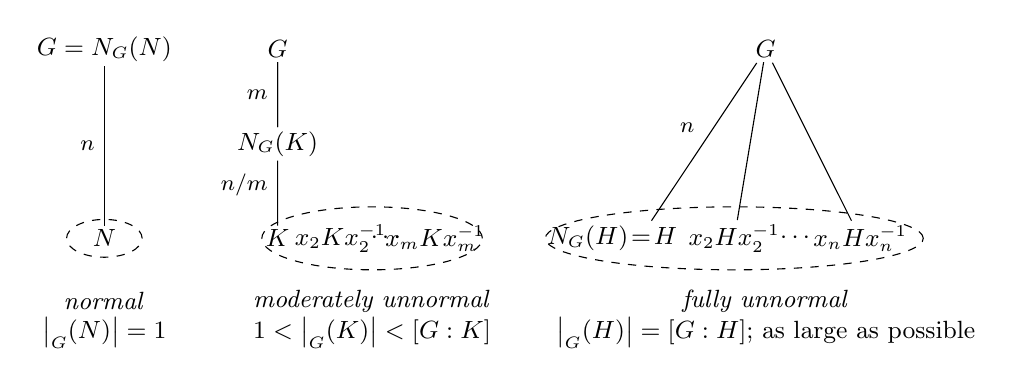
\begin{tikzpicture}[scale=.8]
    %%
    \tikzstyle{every node}=[font=\small]
    %%
    \begin{scope}[shift={(0,0)},shorten >= -2pt, shorten <= -2pt]
      \node (G) at (0,3) {$G=\Balert{N_G(N)}$};
      \node (N) at (0,0) {$N$};
      \draw (G)--(N) node[left,pos=.5] {\footnotesize $n$};
      \draw[dashed] (0,0) circle [x radius=.6cm, y radius=.3cm];
      \node at (0,-1) {\Balert{\emph{normal}}};
      \node at (0,-1.5) {$\big|\cl_G(N)\big|=1$};
    \end{scope}
    %%
    \begin{scope}[shift={(4.25,0)},shorten >= -2pt, shorten <= -2pt]
      \node (G) at (-1.5,3) {$G$};
      \node (N_G) at (-1.5,1.5) {\Palert{$N_G(K)$}};
      \node (K) at (-1.5,0) {$K$};
      \node (K2) at (-.5,0) {$x_2Kx_2^{-1}$};
      \node (K3) at (.25,0) {$\cdots$};
      \node (Kl) at (1,0) {$x_m Kx_m^{-1}$};
      \draw (G) -- (N_G);
      \draw (N_G) -- (K) node[left,pos=.35] {\footnotesize $n/m$};
      \draw (G)--(N_G) node[left,pos=.5] {\footnotesize $m$};
      \draw[dashed] (0,0) circle [x radius=1.75cm, y radius=.5cm];
      \node at (0,-1) {\Palert{\emph{moderately unnormal}}};
      \node at (0,-1.5) {$1<\big|\cl_G(K)\big|<[G:K]$};
    \end{scope}
    %%
    \begin{scope}[shift={(10.5,0)},shorten >= -2pt, shorten <= -2pt]
      \node (G) at (0,3) {$G$};
      \node (H) at (-2,0) {\hspace{-7mm}$\Alert{N_G(H)}\!=\!H$};
      \node (H2) at (-.5,0) {$x_2Hx_2^{-1}$};
      \node (H3) at (.5,0) {$\cdots$};
      \node (Hl) at (1.5,0) {$x_n Hx_n^{-1}$};
      \draw (G)--(H) node[above left,pos=.5] {\footnotesize $n$};
      \draw (G) -- (H2); \draw (G) -- (Hl);
      \draw[dashed] (-.5,0) circle [x radius=3cm, y radius=.5cm];
      \node at (0,-1) {\Alert{\emph{fully unnormal}}};
      \node at (0,-1.5) {$\big|\cl_G(H)\big|=[G:H]$; as large as possible};
    \end{scope}
  \end{tikzpicture}
  \]
  
\end{frame}

%%====================================================================

\begin{frame}[t]{``Reducing'' subgroup lattices} %\pause

  Sometimes it is convenient to collapse conjugacy classes into single
  nodes in the lattice. \medskip\pause
  
  We'll call this the \Alert{subgroup diagram}
  (\emph{caveat}: it need not be a lattice!). Sometimes it reveals
  patterns in new ways. \medskip\pause
  
  Here are the subgroup diagrams of the \Balert{dihedral groups}. (Note that
  $D_2\cong V_4$.)
  %%
  %% Subgroup diagrams of the dihedral groups 
  \[
  \begin{tikzpicture}[scale=.9]
    %%
    \tikzstyle{every node}=[font=\small]
    %%
    \begin{scope}[shift={(0,0)}]
      \node (D2) at (0,3) {$D_2$};
      \node (C2-l) at (-1,2) {$C_2$};
      \node (C2-m) at (0,2) {$C_2$};
      \node (C2-r) at (1,2) {$C_2$};
      \node (C1) at (0,1) {$C_1$};
      \draw[f] (D2) to (C2-l); \draw[f] (D2) to (C2-m); \draw[f] (D2) to (C2-r);
      \draw[f] (C2-l) to (C1); \draw[f] (C2-m) to (C1); \draw[f] (C2-r) to (C1);
    \end{scope}
    %%
    \begin{scope}[shift={(3.25,0)}]
      \node (Q16) at (0,4) {$D_4$};
      \node (C8) at (0,3) {$C_4$};
      \node (C4) at (0,2) {$C_2$};
      \node (C2) at (0,1) {$C_1$};
      \node (Q8-l) at (-1,3) {$D_2$};
      \node (C4-l) at (-1,2) {${}_{\color{midgray} 2}C_2$};
      \node (Q8-r) at (1,3) {$D_2$};
      \node (C4-r) at (1,2) {${}_{\color{midgray} 2}C_2$};
      \draw[f] (Q16) to (C8);
      \draw[f] (C8) to (C4);
      \draw[f] (C4) to (C2);
      \draw[f] (Q16) to (Q8-l); \draw[f] (Q16) to (Q8-r); 
      \draw[f] (Q8-l) to (C4-l); \draw[f] (Q8-r) to (C4-r); 
      \draw[f] (Q8-l) to (C4); \draw[f] (Q8-r) to (C4);
      \draw[f] (C4-l) to (C2); \draw[f] (C4-r) to (C2);
    \end{scope}
    %%
    \begin{scope}[shift={(6.5,0)}]
      \node (Q32) at (0,5) {$D_8$};
      \node (C16) at (0,4) {$C_8$};
      \node (C8) at (0,3) {$C_4$};
      \node (C4) at (0,2) {$C_2$};
      \node (C2) at (0,1) {$C_1$};
      \node (Q16-l) at (-1,4) {$D_4$};
      \node (Q8-l) at (-1,3) {${}_{\color{midgray} 2}D_2$};
      \node (C4-l) at (-1,2) {${}_{\color{midgray} 4}C_2$};
      \node (Q16-r) at (1,4) {$D_4$};
      \node (Q8-r) at (1,3) {${}_{\color{midgray} 2}D_2$};
      \node (C4-r) at (1,2) {${}_{\color{midgray} 4}C_2$};
      \draw[f] (Q32) to (C16);
      \draw[f] (C16) to (C8);
      \draw[f] (C8) to (C4);
      \draw[f] (C4) to (C2);
      \draw[f] (Q32) to (Q16-l); \draw[f] (Q32) to (Q16-r); 
      \draw[f] (Q16-l) to (Q8-l); \draw[f] (Q16-r) to (Q8-r); 
      \draw[f] (Q8-l) to (C4-l); \draw[f] (Q8-r) to (C4-r); 
      \draw[f] (Q16-l) to (C8); \draw[f] (Q16-r) to (C8);
      \draw[f] (Q8-l) to (C4); \draw[f] (Q8-r) to (C4);
      \draw[f] (C4-l) to (C2); \draw[f] (C4-r) to (C2);
    \end{scope}
    %%
    \begin{scope}[shift={(9.75,0)}]
      \node (Q64) at (0,6) {$D_{16}$};
      \node (C32) at (0,5) {$C_{16}$};
      \node (C16) at (0,4) {$C_8$};
      \node (C8) at (0,3) {$C_4$};
      \node (C4) at (0,2) {$C_2$};
      \node (C2) at (0,1) {$C_1$};
      \node (Q32-l) at (-1,5) {$D_8$};
      \node (Q16-l) at (-1,4) {${}_{\color{midgray} 2}D_4$};
      \node (Q8-l) at (-1,3) {${}_{\color{midgray} 4}D_2$};
      \node (C4-l) at (-1,2) {${}_{\color{midgray} 8}C_2$};
      \node (Q32-r) at (1,5) {$D_8$};
      \node (Q16-r) at (1,4) {${}_{\color{midgray} 2}D_4$};
      \node (Q8-r) at (1,3) {${}_{\color{midgray} 4}D_2$};
      \node (C4-r) at (1,2) {${}_{\color{midgray} 8}C_2$};
      \draw[f] (Q64) to (C32);
      \draw[f] (C32) to (C16);
      \draw[f] (C16) to (C8);
      \draw[f] (C8) to (C4);
      \draw[f] (C4) to (C2);
      \draw[f] (Q64) to (Q32-l); \draw[f] (Q64) to (Q32-r);
      \draw[f] (Q32-l) to (Q16-l); \draw[f] (Q32-r) to (Q16-r); 
      \draw[f] (Q16-l) to (Q8-l); \draw[f] (Q16-r) to (Q8-r); 
      \draw[f] (Q8-l) to (C4-l); \draw[f] (Q8-r) to (C4-r); 
      \draw[f] (Q32-l) to (C16); \draw[f] (Q32-r) to (C16);
      \draw[f] (Q16-l) to (C8); \draw[f] (Q16-r) to (C8);
      \draw[f] (Q8-l) to (C4); \draw[f] (Q8-r) to (C4);
      \draw[f] (C4-l) to (C2); \draw[f] (C4-r) to (C2);
    \end{scope}
  \end{tikzpicture}
  \]
  The left-subscript denotes the size.
  
\end{frame}

%%====================================================================

\begin{frame}[t]{``Reducing'' subgroup lattices}
  
  Sometimes it is convenient to collapse conjugacy classes into single
  nodes in the lattice. \medskip\pause
  
  We'll call this the \Alert{subgroup diagram}
  (\emph{caveat}: it need not be a lattice!). Sometimes it reveals
  patterns in new ways. \medskip\pause

  Here are the subgroup diagrams of the \Balert{generalized quaternion} groups.
  What do you notice?
  %%
  %% Subgroup diagrams of the generalized quaternion groups
  \[
  \begin{tikzpicture}[scale=.9]
    %%
    \tikzstyle{every node}=[font=\small]
    %%
    \begin{scope}[shift={(0,0)}]
      \node (Q8) at (0,3) {$Q_8$};
      \node (C4) at (0,2) {$C_4$};
      \node (C2) at (0,1) {$C_2$};
      \node (1) at (0,0) {$C_1$};
      \node (C4-l) at (-1,2) {$C_4$};
      \node (C4-r) at (1,2) {$C_4$};
      \draw[f] (Q8) to (C4);
      \draw[f] (C4) to (C2);
      \draw[f] (C2) to (1);
      \draw[f] (Q8) to (C4-l); \draw[f] (Q8) to (C4-r); 
      \draw[f] (C4-l) to (C2); \draw[f] (C4-r) to (C2);
    \end{scope}
    %%
    \begin{scope}[shift={(3.25,0)}]
      \node (Q16) at (0,4) {$Q_{16}$};
      \node (C8) at (0,3) {$C_8$};
      \node (C4) at (0,2) {$C_4$};
      \node (C2) at (0,1) {$C_2$};
      \node (1) at (0,0) {$C_1$};
      \node (Q8-l) at (-1,3) {$Q_8$};
      \node (C4-l) at (-1,2) {${}_{\color{midgray} 2}C_4$};
      \node (Q8-r) at (1,3) {$Q_8$};
      \node (C4-r) at (1,2) {${}_{\color{midgray} 2}C_4$};
      \draw[f] (Q16) to (C8);
      \draw[f] (C8) to (C4);
      \draw[f] (C4) to (C2);
      \draw[f] (C2) to (1);
      \draw[f] (Q16) to (Q8-l); \draw[f] (Q16) to (Q8-r); 
      \draw[f] (Q8-l) to (C4-l); \draw[f] (Q8-r) to (C4-r); 
      \draw[f] (Q8-l) to (C4); \draw[f] (Q8-r) to (C4);
      \draw[f] (C4-l) to (C2); \draw[f] (C4-r) to (C2);
    \end{scope}
    %%
    \begin{scope}[shift={(6.5,0)}]
      \node (Q32) at (0,5) {$Q_{32}$};
      \node (C16) at (0,4) {$C_{16}$};
      \node (C8) at (0,3) {$C_8$};
      \node (C4) at (0,2) {$C_4$};
      \node (C2) at (0,1) {$C_2$};
      \node (1) at (0,0) {$C_1$};
      \node (Q16-l) at (-1,4) {$Q_{16}$};
      \node (Q8-l) at (-1,3) {${}_{\color{midgray} 2}Q_8$};
      \node (C4-l) at (-1,2) {${}_{\color{midgray} 4}C_4$};
      \node (Q16-r) at (1,4) {$Q_{16}$};
      \node (Q8-r) at (1,3) {${}_{\color{midgray} 2}Q_8$};
      \node (C4-r) at (1,2) {${}_{\color{midgray} 4}C_4$};
      \draw[f] (Q32) to (C16);
      \draw[f] (C16) to (C8);
      \draw[f] (C8) to (C4);
      \draw[f] (C4) to (C2);
      \draw[f] (C2) to (1);
      \draw[f] (Q32) to (Q16-l); \draw[f] (Q32) to (Q16-r); 
      \draw[f] (Q16-l) to (Q8-l); \draw[f] (Q16-r) to (Q8-r); 
      \draw[f] (Q8-l) to (C4-l); \draw[f] (Q8-r) to (C4-r); 
      \draw[f] (Q16-l) to (C8); \draw[f] (Q16-r) to (C8);
      \draw[f] (Q8-l) to (C4); \draw[f] (Q8-r) to (C4);
      \draw[f] (C4-l) to (C2); \draw[f] (C4-r) to (C2);
    \end{scope}
    %%
    \begin{scope}[shift={(9.75,0)}]
      \node (Q64) at (0,6) {$Q_{64}$};
      \node (C32) at (0,5) {$C_{32}$};
      \node (C16) at (0,4) {$C_{16}$};
      \node (C8) at (0,3) {$C_8$};
      \node (C4) at (0,2) {$C_4$};
      \node (C2) at (0,1) {$C_2$};
      \node (1) at (0,0) {$C_1$};
      \node (Q32-l) at (-1,5) {$Q_{32}$};
      \node (Q16-l) at (-1,4) {${}_{\color{midgray} 2}Q_{16}$};
      \node (Q8-l) at (-1,3) {${}_{\color{midgray} 4}Q_8$};
      \node (C4-l) at (-1,2) {${}_{\color{midgray} 8}C_4$};
      \node (Q32-r) at (1,5) {$Q_{32}$};
      \node (Q16-r) at (1,4) {${}_{\color{midgray} 2}Q_{16}$};
      \node (Q8-r) at (1,3) {${}_{\color{midgray} 4}Q_8$};
      \node (C4-r) at (1,2) {${}_{\color{midgray} 8}C_4$};
      \draw[f] (Q64) to (C32);
      \draw[f] (C32) to (C16);
      \draw[f] (C16) to (C8);
      \draw[f] (C8) to (C4);
      \draw[f] (C4) to (C2);
      \draw[f] (C2) to (1);
      \draw[f] (Q64) to (Q32-l); \draw[f] (Q64) to (Q32-r);
      \draw[f] (Q32-l) to (Q16-l); \draw[f] (Q32-r) to (Q16-r); 
      \draw[f] (Q16-l) to (Q8-l); \draw[f] (Q16-r) to (Q8-r); 
      \draw[f] (Q8-l) to (C4-l); \draw[f] (Q8-r) to (C4-r); 
      \draw[f] (Q32-l) to (C16); \draw[f] (Q32-r) to (C16);
      \draw[f] (Q16-l) to (C8); \draw[f] (Q16-r) to (C8);
      \draw[f] (Q8-l) to (C4); \draw[f] (Q8-r) to (C4);
      \draw[f] (C4-l) to (C2); \draw[f] (C4-r) to (C2);
    \end{scope}
  \end{tikzpicture}
  \]
  
\end{frame}

%%====================================================================

\begin{frame}{Normal subgroups of order $2$} %\Pause

  Often, we can determine the normal subgroups and conjugacy
  classes simply from inspecting the subgroup lattice. \medskip\Pause

  We'll make frequent use of the following straightforward result. 
  
  \medskip\Pause
  
  \begin{block}{Lemma}
    A subgroup $H$ of order $2$ is normal if and only if it is contained in
    $Z(G)$.
  \end{block}

  \begin{exampleblock}{Proof} \Pause
    Let $H=\{e,h\}$. \medskip\Pause

    ``$\Leftarrow$'': \Pause We already know that subgroups contained in
    $Z(G)$ are normal. $\hfill\checkmark$ \medskip\Pause
    
    ``$\Rightarrow$'': Suppose $H\normaleq G$. \Pause Then for all $x\in G$,
    \[
    xH\Pause=x\{e,h\}\Pause=\{x,xh\},\Pause\quad\text{and}\quad
    Hx\Pause=\{e,h\}x\Pause=\{x,hx\}. 
    \]
    \Pause Since $xH=Hx$, we must have $xh=hx$, and hence $H\leq
    Z(G)$. $\hfill\checkmark$ \medskip\Pause
  \end{exampleblock}
  
\end{frame}

%%====================================================================

\begin{frame}{Unicorn subgroups}

  Suppose we conjugate $G=D_4$ by some element $x\in D_4$. \vspace{-2mm}
  
  %% Subgroup lattice of D_4 and conjugating it by an element x
  \[
  \begin{tikzpicture}[scale=.92]
    %%
    \tikzstyle{every node}=[font=\small]
    %%
    \begin{scope}[shift={(0,0)},shorten >= -3pt, shorten <= -3pt]
      \node (D4) at (0,4) {\Palert{$D_4$}};
      \node (r2-f) at (-1.25,3) {$\<r^2,f\>$};
      \node (r) at (0,3) {\Palert{$\<r\>$}};
      \node (r2-rf) at (1.25,3) {$\<r^2,rf\>$};
      \node (f) at (-2.5,2) {$\<f\>$};
      \node (r2f) at (-1.25,2) {$\<r^2f\>$};
      \node (r2) at (0,2) {\Palert{$\<r^2\>$}};
      \node (r3f) at (1.25,2) {$\<r^3f\>$};
      \node (rf) at (2.5,2) {$\<rf\>$};
      \node (1) at (0,1) {\Palert{$\<1\>$}};
      %%
      \draw[f] (D4) to (r2-f); \draw[f] (D4) to (r); \draw[f] (D4) to (r2-rf);
      \draw[f] (r2-f) to (f); \draw[f] (r2-f) to (r2f); \draw[f] (r2-f) to (r2);
      \draw[f] (r2-rf) to (rf); \draw[f] (r2-rf) to (r3f);
      \draw[f] (r2-rf) to (r2);
      \draw[f] (r2) to (r); \draw[f] (r2) to (1); \draw[f] (f) to (1);
      \draw[f] (r2f) to (1); \draw[f] (r3f) to (1); \draw[f] (rf) to (1);
      \draw[dashed,midgray] (0,4) circle [x radius=.4cm, y radius=.3cm];
      \draw[dashed,midgray] (-1.25,3) circle [x radius=.6cm, y radius=.3cm];
      \draw[dashed,midgray] (1.25,3) circle [x radius=.6cm, y radius=.3cm];
      \draw[dashed,midgray] (0,3) circle [x radius=.4cm, y radius=.3cm];
      \draw[dashed,midgray] (0,2) circle [x radius=.4cm, y radius=.3cm];
      \draw[dashed,midgray] (0,1) circle [x radius=.4cm, y radius=.3cm];
    \end{scope}
    %%
    \begin{scope}[shift={(6.25,0)},shorten >= -3pt, shorten <= -3pt]
      \node (D4) at (0,4) {\Palert{$xD_4x^{-1}$}};
      \node (r2-f) at (-1.25,3) {$x\<r^2,f\>x^{-1}$};
      \node (r) at (0,3) {\Palert{$x\<r\>x^{-1}$}};
      \node (r2-rf) at (1.25,3) {$x\<r^2,rf\>x^{-1}$};
      \node (f) at (-2.5,2) {$x\<f\>x^{-1}$};
      \node (r2f) at (-1.25,2) {$x\<r^2f\>x^{-1}$};
      \node (r2) at (0,2) {\Palert{$x\<r^2\>x^{-1}$}};
      \node (r3f) at (1.25,2) {$x\<r^3f\>x^{-1}$};
      \node (rf) at (2.5,2) {$x\<rf\>x^{-1}$};
      \node (1) at (0,1) {\Palert{$x\<1\>x^{-1}$}};
      %%
      \draw[f] (D4) to (r2-f); \draw[f] (D4) to (r); \draw[f] (D4) to (r2-rf);
      \draw[f] (r2-f) to (f); \draw[f] (r2-f) to (r2f); \draw[f] (r2-f) to (r2);
      \draw[f] (r2-rf) to (rf); \draw[f] (r2-rf) to (r3f);
      \draw[f] (r2-rf) to (r2);
      \draw[f] (r2) to (r); \draw[f] (r2) to (1); \draw[f] (f) to (1);
      \draw[f] (r2f) to (1); \draw[f] (r3f) to (1); \draw[f] (rf) to (1);
    \end{scope}
  \end{tikzpicture}
  \]
  \Pause Subgroups at a unique ``lattice neighborhood'' are called
  \Palert{unicorns}, and must be normal. \medskip\Pause
  
  For example, $\Palert{\<r^2\>}=\Palert{x\<r^2\>x^{-1}}$ is the only 
  size-$2$ subgroup ``\emph{\Balert{with $3$ parents}}.'' \medskip\Pause
  
  The groups \Palert{$G$} and \Palert{$\<1\>$} are always
  unicorns, and hence normal. \medskip\Pause
  
  The index-$2$ subgroups $\<r^2,f\>$, \Palert{$\<r\>$}, and
  $\<r^2,rf\>$ must be normal. 
  
  \smallskip\Pause
  
  \begin{exampleblock}{Remark}
    Conjugating a normal subgroup $N\leq G$ by $x\in G$ shuffles its
    elements and subgroups.
  \end{exampleblock}
  
\end{frame}

%%====================================================================

\begin{frame}{Conjugating normal subgroups}

  \begin{block}{Proposition}
    If $H\leq N\normaleq G$, then $xHx^{-1}\leq N$ for all $x\in G$.
  \end{block}
  
  \vspace{-1mm}\Pause
  
  \begin{exampleblock}{Proof}
    Conjugating $H\leq N$ by $x\in G$ yields\; $xHx^{-1}\leq xNx^{-1}\Pause=N$.
    $\hfill\Box$
  \end{exampleblock}
  
  \vspace{-3mm}\Pause
  
  %% Subgroup lattice of N\leq D_4 and conjugating it by an element x
  \[
  \begin{tikzpicture}[scale=.6]
    %%  
    \tikzstyle{v-r}=[circle,draw,fill=vRed,inner sep=0pt,minimum size=1.75mm]
    \tikzstyle{v-g}=[circle,draw,fill=vGreen,inner sep=0pt,minimum size=1.75mm]
    \tikzstyle{v-b}=[circle,draw,fill=vBlue,inner sep=0pt,minimum size=1.75mm]
    \tikzstyle{v-p}=[circle,draw,fill=vPurple,inner sep=0pt,minimum size=1.75mm]
    \tikzstyle{v-w}=[circle,draw,fill=white,inner sep=0pt,minimum size=1.75mm]
    \tikzstyle{v-fad}=[circle,draw,faded,fill=white,inner sep=0pt,minimum size=1.75mm]
    \tikzstyle{v-gr}=[circle,draw,fill=midgray,inner sep=0pt,minimum size=1.75mm]
    \tikzstyle{cy2-r} = [draw, thick,bend right=12]
    \tikzstyle{cy2-fad} = [draw,faded,thick]    
    \tikzstyle{lat} = [draw,very thick,faded,shorten >= 3pt, shorten <= 3pt]
    %%
    \begin{scope}[shift={(0,0)}]
      \begin{scope}[shift={(0,6.5)},scale=.4]
        \node (1) at (90:2) [v-gr] {};
        \node (r) at (180:2) [v-w] {};
        \node (r2) at (270:2) [v-p] {};
        \node (r3) at (0:2) [v-w] {};
        \node (f) at (-1.8,3.3) [v-b] {};
        \node (r2f) at (-.6,3.3) [v-b] {};
        \node (rf) at (.6,3.3) [v-fad] {};
        \node (r3f) at (1.8,3.3) [v-fad] {};
        \draw [cy2-r] (1) to [bend right=30] (r);
        \draw [cy2-r] (r) to [bend right=30] (r2);
        \draw [cy2-r] (r2) to [bend right=30] (r3);
        \draw [cy2-r] (r3) to [bend right=30] (1);
        \draw [cy2] (1) to (f);
        \draw [cy2-fad] (1) to (rf);
        \draw [cy2] (1) to (r2f);
        \draw [cy2-fad] (1) to (r3f);
        \node at (0,0) {$N$};
        \node (r2-f-top) at (0,3.5) {};
        \node (r2-f-bot) at (0,-2) {};
      \end{scope}
      %%
      \begin{scope}[shift={(-2.75,3.25)},scale=.4]
        \node (1) at (90:2) [v-gr] {};
        \node (r) at (180:2) [v-fad] {};
        \node (r2) at (270:2) [v-fad] {};
        \node (r3) at (0:2) [v-fad] {};
        \node (f) at (-1.8,3.3) [v-b] {};
        \node (r2f) at (-.6,3.3) [v-fad] {};
        \node (rf) at (.6,3.3) [v-fad] {};
        \node (r3f) at (1.8,3.3) [v-fad] {};
        \draw [cy2-fad] (1) to [bend right=30] (r);
        \draw [cy2-fad] (r) to [bend right=30] (r2);
        \draw [cy2-fad] (r2) to [bend right=30] (r3);
        \draw [cy2-fad] (r3) to [bend right=30] (1);
        \draw [cy2] (1) to (f);
        \draw [cy2-fad] (1) to (rf);
        \draw [cy2-fad] (1) to (r2f);
        \draw [cy2-fad] (1) to (r3f);
        \node at (0,0) {\Alert{$\<f\>$}};
        \node (f-top) at (0,3.7) {};
        \node (f-bot) at (0,-2) {};
      \end{scope}
      %%
      \begin{scope}[shift={(0,3.25)},scale=.4]
        \node (1) at (90:2) [v-gr] {};
        \node (r) at (180:2) [v-fad] {};
        \node (r2) at (270:2) [v-fad] {};
        \node (r3) at (0:2) [v-fad] {};
        \node (f) at (-1.8,3.3) [v-fad] {};
        \node (r2f) at (-.6,3.3) [v-b] {};
        \node (rf) at (.6,3.3) [v-fad] {};
        \node (r3f) at (1.8,3.3) [v-fad] {};
        \draw [cy2-fad] (1) to [bend right=30] (r);
        \draw [cy2-fad] (r) to [bend right=30] (r2);
        \draw [cy2-fad] (r2) to [bend right=30] (r3);
        \draw [cy2-fad] (r3) to [bend right=30] (1);
        \draw [cy2-fad] (1) to (f);
        \draw [cy2-fad] (1) to (rf);
        \draw [cy2] (1) to (r2f);
        \draw [cy2-fad] (1) to (r3f);
        \node at (0,0) {\Alert{$\<r^2f\>$}};
        \node (r2f-top) at (0,3.7) {};
        \node (r2f-bot) at (0,-2) {};
      \end{scope}
      %%
      \begin{scope}[shift={(2.75,3.25)},scale=.4]
        \node (1) at (90:2) [v-gr] {};
        \node (r) at (180:2) [v-w] {};
        \node (r2) at (270:2) [v-p] {};
        \node (r3) at (0:2) [v-w] {};
        \node (f) at (-1.8,3.3) [v-fad] {};
        \node (r2f) at (-.6,3.3) [v-fad] {};
        \node (rf) at (.6,3.3) [v-fad] {};
        \node (r3f) at (1.8,3.3) [v-fad] {};
        \draw [cy2-r] (1) to [bend right=30] (r);
        \draw [cy2-r] (r) to [bend right=30] (r2);
        \draw [cy2-r] (r2) to [bend right=30] (r3);
        \draw [cy2-r] (r3) to [bend right=30] (1);
        \draw [cy2-fad] (1) to (f);
        \draw [cy2-fad] (1) to (rf);
        \draw [cy2-fad] (1) to (r2f);
        \draw [cy2-fad] (1) to (r3f);
        \node at (0,0) {\Palert{$\<r^2\>$}};
        \node (r2-top) at (0,3.7) {};
        \node (r2-bot) at (0,-2) {};
      \end{scope}
      %%
      \begin{scope}[shift={(0,0)},scale=.4]
        \node (1) at (90:2) [v-gr] {};
        \node (r) at (180:2) [v-fad] {};
        \node (r2) at (270:2) [v-fad] {};
        \node (r3) at (0:2) [v-fad] {};
        \node (f) at (-1.8,3.3) [v-fad] {};
        \node (r2f) at (-.6,3.3) [v-fad] {};
        \node (rf) at (.6,3.3) [v-fad] {};
        \node (r3f) at (1.8,3.3) [v-fad] {};
        \draw [cy2-fad] (1) to [bend right=30] (r);
        \draw [cy2-fad] (r) to [bend right=30] (r2);
        \draw [cy2-fad] (r2) to [bend right=30] (r3);
        \draw [cy2-fad] (r3) to [bend right=30] (1);
        \draw [cy2-fad] (1) to (f);
        \draw [cy2-fad] (1) to (rf);
        \draw [cy2-fad] (1) to (r2f);
        \draw [cy2-fad] (1) to (r3f);
        \node at (0,0) {\Palert{$\<1\>$}};
        \node (1-top) at (0,3.7) {};
      \end{scope}
      %%
      \draw [lat] (r2-f-bot) to (f-top);
      \draw [lat] (r2-f-bot) to (r2f-top);
      \draw [lat] (r2-f-bot) to (r2-top);
      \draw [lat] (f-bot) to (1-top);
      \draw [lat] (r2f-bot) to (1-top);
      \draw [lat] (r2-bot) to (1-top);  
    \end{scope}
    %%
    %%
    %%
    \begin{scope}[shift={(8.5,0)}]
      \begin{scope}[shift={(0,6.5)},scale=.4]
        %%
        \tikzstyle{every node}=[font=\small]
        %%
        \node (1) at (90:2) [v-gr] {};
        \node (r) at (180:2) [v-w] {};
        \node (r2) at (270:2) [v-p] {};
        \node (r3) at (0:2) [v-w] {};
        \node (f) at (-1.8,3.3) [v-b] {};
        \node (r2f) at (-.6,3.3) [v-b] {};
        \node (rf) at (.6,3.3) [v-fad] {};
        \node (r3f) at (1.8,3.3) [v-fad] {};
        \draw [cy2-r] (1) to [bend right=30] (r);
        \draw [cy2-r] (r) to [bend right=30] (r2);
        \draw [cy2-r] (r2) to [bend right=30] (r3);
        \draw [cy2-r] (r3) to [bend right=30] (1);
        \draw [cy2] (1) to (f);
        \draw [cy2-fad] (1) to (rf);
        \draw [cy2] (1) to (r2f);
        \draw [cy2-fad] (1) to (r3f);
        \node at (0,0) {$xNx^{-1}$};
        \node (r2-f-top) at (0,3.7) {};
        \node (r2-f-bot) at (0,-2) {};
      \end{scope}
      %%
      \begin{scope}[shift={(-2.75,3.25)},scale=.4]
        %%
        \tikzstyle{every node}=[font=\footnotesize]
        %%
        \node (1) at (90:2) [v-gr] {};
        \node (r) at (180:2) [v-fad] {};
        \node (r2) at (270:2) [v-fad] {};
        \node (r3) at (0:2) [v-fad] {};
        \node (f) at (-1.8,3.3) [v-w] {};
        \node (r2f) at (-.6,3.3) [v-w] {};
        \node (rf) at (.6,3.3) [v-fad] {};
        \node (r3f) at (1.8,3.3) [v-fad] {};
        \draw [cy2-fad] (1) to [bend right=30] (r);
        \draw [cy2-fad] (r) to [bend right=30] (r2);
        \draw [cy2-fad] (r2) to [bend right=30] (r3);
        \draw [cy2-fad] (r3) to [bend right=30] (1);
        \draw [cy2] (1) to (f);
        \draw [cy2-fad] (1) to (rf);
        \draw [cy2] (1) to (r2f);
        \draw [cy2-fad] (1) to (r3f);
        \node at (0,0) {\Alert{$x\<f\>x^{-1}$}};
        \node (f-top) at (0,3.7) {};
        \node (f-bot) at (0,-2) {};
      \end{scope}
      %%
      \begin{scope}[shift={(0,3.25)},scale=.4]
        %%
        \tikzstyle{every node}=[font=\tiny]
        %%
        \node (1) at (90:2) [v-gr] {};
        \node (r) at (180:2) [v-fad] {};
        \node (r2) at (270:2) [v-fad] {};
        \node (r3) at (0:2) [v-fad] {};
        \node (f) at (-1.8,3.3) [v-w] {};
        \node (r2f) at (-.6,3.3) [v-w] {};
        \node (rf) at (.6,3.3) [v-fad] {};
        \node (r3f) at (1.8,3.3) [v-fad] {};
        \draw [cy2-fad] (1) to [bend right=30] (r);
        \draw [cy2-fad] (r) to [bend right=30] (r2);
        \draw [cy2-fad] (r2) to [bend right=30] (r3);
        \draw [cy2-fad] (r3) to [bend right=30] (1);
        \draw [cy2] (1) to (f);
        \draw [cy2-fad] (1) to (rf);
        \draw [cy2] (1) to (r2f);
        \draw [cy2-fad] (1) to (r3f);
        \node at (0,0) {\Alert{$x\<r^2\!f\>x^{-1}$}};
        \node (r2f-top) at (0,3.7) {};
        \node (r2f-bot) at (0,-2) {};
      \end{scope}
      %%
      \begin{scope}[shift={(2.75,3.25)},scale=.4]
        %%
        \tikzstyle{every node}=[font=\scriptsize]
        %%
        \node (1) at (90:2) [v-gr] {};
        \node (r) at (180:2) [v-w] {};
        \node (r2) at (270:2) [v-p] {};
        \node (r3) at (0:2) [v-w] {};
        \node (f) at (-1.8,3.3) [v-fad] {};
        \node (r2f) at (-.6,3.3) [v-fad] {};
        \node (rf) at (.6,3.3) [v-fad] {};
        \node (r3f) at (1.8,3.3) [v-fad] {};
        \draw [cy2-r] (1) to [bend right=30] (r);
        \draw [cy2-r] (r) to [bend right=30] (r2);
        \draw [cy2-r] (r2) to [bend right=30] (r3);
        \draw [cy2-r] (r3) to [bend right=30] (1);
        \draw [cy2-fad] (1) to (f);
        \draw [cy2-fad] (1) to (rf);
        \draw [cy2-fad] (1) to (r2f);
        \draw [cy2-fad] (1) to (r3f);
        \node at (0,0) {\Palert{$x\<r^2\>x^{-1}$}};
        \node (r2-top) at (0,3.7) {};
        \node (r2-bot) at (0,-2) {};
      \end{scope}
      %%
      \begin{scope}[shift={(0,0)},scale=.4]
        %%
        \tikzstyle{every node}=[font=\footnotesize]
        %%
        \node (1) at (90:2) [v-gr] {};
        \node (r) at (180:2) [v-fad] {};
        \node (r2) at (270:2) [v-fad] {};
        \node (r3) at (0:2) [v-fad] {};
        \node (f) at (-1.8,3.3) [v-fad] {};
        \node (r2f) at (-.6,3.3) [v-fad] {};
        \node (rf) at (.6,3.3) [v-fad] {};
        \node (r3f) at (1.8,3.3) [v-fad] {};
        \draw [cy2-fad] (1) to [bend right=30] (r);
        \draw [cy2-fad] (r) to [bend right=30] (r2);
        \draw [cy2-fad] (r2) to [bend right=30] (r3);
        \draw [cy2-fad] (r3) to [bend right=30] (1);
        \draw [cy2-fad] (1) to (f);
        \draw [cy2-fad] (1) to (rf);
        \draw [cy2-fad] (1) to (r2f);
        \draw [cy2-fad] (1) to (r3f);
        \node at (0,0) {\Palert{$x\<1\>x^{-1}$}};
        \node (1-top) at (0,3.7) {};
      \end{scope}
      %%
      \draw [lat] (r2-f-bot) to (f-top);
      \draw [lat] (r2-f-bot) to (r2f-top);
      \draw [lat] (r2-f-bot) to (r2-top);
      \draw [lat] (f-bot) to (1-top);
      \draw [lat] (r2f-bot) to (1-top);
      \draw [lat] (r2-bot) to (1-top);  
    \end{scope}
  \end{tikzpicture}
  \]
  
\end{frame}

%%====================================================================

\begin{frame}{Determining the conjugacy classes from the subgroup lattice}

  Suppose we conjugate $G=D_4$ by some element $x\in D_4$. \vspace{-2mm}

  %% Subgroup lattice of D_4 and a conjugate by x
  \[
  \begin{tikzpicture}[scale=.92]
    %%
    \tikzstyle{every node}=[font=\small]
    %%
    \begin{scope}[shift={(0,0)},shorten >= -3pt, shorten <= -3pt]
      \node (D4) at (0,4) {\Palert{$D_4$}};
      \node (r2-f) at (-1.25,3) {$\<r^2,f\>$};
      \node (r) at (0,3) {\Palert{$\<r\>$}};
      \node (r2-rf) at (1.25,3) {$\<r^2,rf\>$};
      \node (f) at (-2.5,2) {$\<f\>$};
      \node (r2f) at (-1.25,2) {$\<r^2f\>$};
      \node (r2) at (0,2) {\Palert{$\<r^2\>$}};
      \node (r3f) at (1.25,2) {$\<r^3f\>$};
      \node (rf) at (2.5,2) {$\<rf\>$};
      \node (1) at (0,1) {\Palert{$\<1\>$}};
      %%
      \draw[f] (D4) to (r2-f); \draw[f] (D4) to (r); \draw[f] (D4) to (r2-rf);
      \draw[f] (r2-f) to (f); \draw[f] (r2-f) to (r2f); \draw[f] (r2-f) to (r2);
      \draw[f] (r2-rf) to (rf); \draw[f] (r2-rf) to (r3f);
      \draw[f] (r2-rf) to (r2);
      \draw[f] (r2) to (r); \draw[f] (r2) to (1); \draw[f] (f) to (1);
      \draw[f] (r2f) to (1); \draw[f] (r3f) to (1); \draw[f] (rf) to (1);
      \draw[dashed,midgray] (0,4) circle [x radius=.4cm, y radius=.3cm];
      \draw[dashed,midgray] (-1.25,3) circle [x radius=.6cm, y radius=.3cm];
      \draw[dashed,midgray] (1.25,3) circle [x radius=.6cm, y radius=.3cm];
      \draw[dashed,midgray] (0,3) circle [x radius=.4cm, y radius=.3cm];
      \draw[dashed,midgray] (-1.8,2) circle [x radius=1cm, y radius=.4cm];
      \draw[dashed,midgray] (1.8,2) circle [x radius=1cm, y radius=.4cm];
      \draw[dashed,midgray] (0,2) circle [x radius=.4cm, y radius=.3cm];
      \draw[dashed,midgray] (0,1) circle [x radius=.4cm, y radius=.3cm];
    \end{scope}
    %%
    \begin{scope}[shift={(6.25,0)},shorten >= -3pt, shorten <= -3pt]
      \node (D4) at (0,4) {\Palert{$xD_4x^{-1}$}};
      \node (r2-f) at (-1.25,3) {$x\<r^2,f\>x^{-1}$};
      \node (r) at (0,3) {\Palert{$x\<r\>x^{-1}$}};
      \node (r2-rf) at (1.25,3) {$x\<r^2,rf\>x^{-1}$};
      \node (f) at (-2.5,2) {$x\<f\>x^{-1}$};
      \node (r2f) at (-1.25,2) {$x\<r^2f\>x^{-1}$};
      \node (r2) at (0,2) {\Palert{$x\<r^2\>x^{-1}$}};
      \node (r3f) at (1.25,2) {$x\<r^3f\>x^{-1}$};
      \node (rf) at (2.5,2) {$x\<rf\>x^{-1}$};
      \node (1) at (0,1) {\Palert{$x\<1\>x^{-1}$}};
      %%
      \draw[f] (D4) to (r2-f); \draw[f] (D4) to (r); \draw[f] (D4) to (r2-rf);
      \draw[f] (r2-f) to (f); \draw[f] (r2-f) to (r2f); \draw[f] (r2-f) to (r2);
      \draw[f] (r2-rf) to (rf); \draw[f] (r2-rf) to (r3f);
      \draw[f] (r2-rf) to (r2);
      \draw[f] (r2) to (r); \draw[f] (r2) to (1); \draw[f] (f) to (1);
      \draw[f] (r2f) to (1); \draw[f] (r3f) to (1); \draw[f] (rf) to (1);
    \end{scope}
  \end{tikzpicture}
  \]
  
  \Pause
  
  \begin{exampleblock}{Conclusions}
    \begin{itemize}
    \item All unicorns and index-$2$ subgroups are normal. \Pause
    \item $\<f\>$ cannot be normal because $f\not\in Z(D_4)$. Thus, it
      has some other conjugate. \Pause
    \item Each conjugate to $\<f\>$ must be contained in
      $\<r^2,f\>$. \Pause Therefore,
      \[
      \cl_{D_4}(\<f\>)=\big\{\<f\>,\<rf\>\big\}=\cl_{D_4}(\<rf\>).
      \] \Pause\vspace{-5mm}
    \item The normalizer of $\<f\>$ must have index $2$, and thus
      $N_{D_4}(\<f\>)=\<r^2,f\>$. \Pause
    \item \emph{We just determined all conjugacy classes and
      normalizers simply by inspection!}
    \end{itemize}
  \end{exampleblock}
  
\end{frame}

%%====================================================================

\begin{frame}{Unicorns in the diquaternion group} %\Pause
  
  Our definition of \Palert{unicorn} could be strengthened, but we
  want to keep things simple. \medskip\Pause
  
  Are any of the $C_4$ subgroups of $\DQ_8$ unicorns, i.e.,
  ``not like the others''? 
  
  %% Subgroup lattice of DQ_8
  \[
  \begin{tikzpicture}[shorten >= -3pt, shorten <= -3pt, scale=1.15]
    \begin{scope}[shift={(0,0)}]
      \node (G) at (0,3) {$\DQ_8$};
      \node (C4xC2-1) at (-3,2) {$C_4\times C_2$}; % 010,001,011
      \node (D4-1) at (-2,2) {$D_4$}; % 100,001,101    
      \node (C4xC2-2) at (-1,2) {$C_4\times C_2$}; % 100,010,110
      \node (D4-2) at (0,2) {$D_4$};  % 100,011,111
      \node (C4xC2-3) at (1,2) {$C_4\times C_2$};  % 010,101,111
      \node (D4-3) at (2,2) {$D_4$};  % 110,001,111
      \node (Q8) at (3,2) {$Q_8$};  % 110,011,101
      %%
      \node (V4-12) at (-3,1) {$V_4$};
      \node (V4-13) at (-2,1) {$V_4$};
      \node (V4-23) at (-1,1) {$V_4$};
      \node (Z) at (0,1) {$C_4$};
      \node (C4-1) at (1,1) {$C_4$};
      \node (C4-2) at (2,1) {$C_4$};
      \node (C4-3) at (3,1) {$C_4$};
      %%
      \node (C2-11) at (-3.25,0) {$C_2$};
      \node (C2-12) at (-2.75,0) {$C_2$};
      \node (C2-21) at (-2.25,0) {$C_2$};
      \node (C2-22) at (-1.75,0) {$C_2$};
      \node (C2-31) at (-1.25,0) {$C_2$};
      \node (C2-32) at (-0.75,0) {$C_2$};    
      \node (-I) at (1,0) {$C_2$};
      %%
      \node (I) at (0,-1) {$\<I\>$};
      %%
      %%
      \draw[f] (C4xC2-1) to (G); \draw[f] (D4-1) to (G);
      \draw[f] (C4xC2-2) to (G);
      \draw[f] (D4-2) to (G); \draw[f] (C4xC2-3) to (G);
      \draw[f] (D4-3) to (G); \draw[f] (Q8) to (G);
      %%
      \draw[f] (C4xC2-1) to (Z); \draw[f] (C4xC2-2) to (Z);
      \draw[f] (C4xC2-3) to (Z); \draw[f] (V4-12) to (D4-1);
      \draw[f] (V4-12) to (D4-2); \draw[f] (V4-12) to (C4xC2-3);
      \draw[f] (V4-13) to (D4-1); \draw[f] (V4-13) to (D4-3);
      \draw[f] (V4-13) to (C4xC2-2); \draw[f] (V4-23) to (D4-2);
      \draw[f] (V4-23) to (D4-3); \draw[f] (V4-23) to (C4xC2-1);
      %%
      \draw[f] (C4-1) to (C4xC2-1); \draw[f] (C4-1) to (D4-1);
      \draw[f] (C4-2) to (C4xC2-2); \draw[f] (C4-2) to (D4-2);
      \draw[f] (C4-3) to (C4xC2-3); \draw[f] (C4-3) to (D4-3);
      %%
      \draw[f] (Q8) to (C4-1); \draw[f] (Q8) to (C4-2); \draw[f] (Q8) to (C4-3);
      %%
      \draw[f] (V4-12) to (C2-11); \draw[f] (V4-12) to (C2-12); 
      \draw[f] (V4-13) to (C2-21); \draw[f] (V4-13) to (C2-22); 
      \draw[f] (V4-23) to (C2-31); \draw[f] (V4-23) to (C2-32); 
      %%
      \draw[f] (-I) to (V4-12); \draw[f] (-I) to (V4-13);
      \draw[f] (-I) to (V4-23); \draw[f] (-I) to (C4-1);
      \draw[f] (-I) to (C4-2); \draw[f] (-I) to (C4-3);
      \draw[f] (-I) to (Z);
      %%
      \draw[f] (C2-11) to (I); \draw[f] (C2-12) to (I); 
      \draw[f] (C2-21) to (I); \draw[f] (C2-22) to (I); 
      \draw[f] (C2-31) to (I); \draw[f] (C2-32) to (I);
      \draw[f] (-I) to (I);
    \end{scope}
  \end{tikzpicture}
  \]
  
  What can we say about the conjugacy classes of the subgroups of
  $\DQ_8$ just from the lattice?
  
\end{frame}

%%====================================================================

\begin{frame}{A mystery group of order $16$} %\Pause

  Let's repeat a previous exercise, for this lattice of an
  actual group. \Palert{Unicorns} are purple.
  %%
  %% Subgroup lattice of a mystery group of order 16
  \[
  \begin{tikzpicture}[shorten >= -2pt, shorten <= -2pt,scale=.65]
    \begin{scope}[shift={(0,0)}]
      \node(G) at (3.5,6) {\Palert{$G$}};
      \node(rs) at (3.5,4.5) {$\<rs\>$};
      \node(r2-s) at (1.75,4.5) {\Palert{$\<r^2,s\>$}};
      \node(r) at (5.25,4.5) {$\<r\>$};
      \node(r4-s) at (0,3) {\Palert{$\<r^4,s\>$}};
      \node(r2s) at (1.75,3) {\Palert{$\<r^2s\>$}};
      \node(r2) at (3.5,3) {\Palert{$\<r^2\>$}};
      \node(s) at (-1.75,1.5) {$\<s\>$};
      \node(r4s) at (0,1.5) {$\<r^4s\>$};
      \node(r4) at (1.75,1.5) {\Palert{$\<r^4\>$}};
      \node(1) at (0,0) {\Palert{$\<1\>$}};
      \draw[f]  (1) to (s);
      \draw[f]  (1) to (r4s);
      \draw[f]  (1) to (r4);
      \draw[f]  (s) to (r4-s);
      \draw[f]  (r4s) to (r4-s);
      \draw[f]  (r4) to (r4-s);
      \draw[f]  (r4) to (r2s);
      \draw[f]  (r4) to (r2);
      \draw[f]  (r4-s) to (r2-s);
      \draw[f]  (r2s) to (r2-s);
      \draw[f]  (r2) to (r2-s);
      \draw[f]  (r2) to (r);
      \draw[f]  (r2) to (rs);
      \draw[f]  (r2-s) to (G);
      \draw[f]  (r) to (G);
      \draw[f]  (rs) to (G);
    \end{scope}
    %%
    \begin{scope}[shift={(8,0)}]
      %%
      \tikzstyle{every node}=[font=\footnotesize]
      %%
      \node(G) at (3.5,6) {\Palert{$xGx^{-1}$}};
      \node(rs) at (3.5,4.5) {$x\<rs\>x^{-1}$};
      \node(r2-s) at (1.75,4.5) {\Palert{$x\<r^2,s\>x^{-1}$}};
      \node(r) at (5.25,4.5) {$x\<r\>x^{-1}$};
      \node(r4-s) at (0,3) {\Palert{$x\<r^4,s\>x^{-1}$}};
      \node(r2s) at (1.75,3) {\Palert{$x\<r^2s\>x^{-1}$}};
      \node(r2) at (3.5,3) {\Palert{$x\<r^2\>x^{-1}$}};
      \node(s) at (-1.75,1.5) {$x\<s\>x^{-1}$};
      \node(r4s) at (0,1.5) {$x\<r^4s\>x^{-1}$};
      \node(r4) at (1.75,1.5) {\Palert{$x\<r^4\>x^{-1}$}};
      \node(1) at (0,0) {\Palert{$x\<1\>x^{-1}$}};
      \draw[f]  (1) to (s);
      \draw[f]  (1) to (r4s);
      \draw[f]  (1) to (r4);
      \draw[f]  (s) to (r4-s);
      \draw[f]  (r4s) to (r4-s);
      \draw[f]  (r4) to (r4-s);
      \draw[f]  (r4) to (r2s);
      \draw[f]  (r4) to (r2);
      \draw[f]  (r4-s) to (r2-s);
      \draw[f]  (r2s) to (r2-s);
      \draw[f]  (r2) to (r2-s);
      \draw[f]  (r2) to (r);
      \draw[f]  (r2) to (rs);
      \draw[f]  (r2-s) to (G);
      \draw[f]  (r) to (G);
      \draw[f]  (rs) to (G);
    \end{scope}
  \end{tikzpicture}
  \]

  \vspace{-2mm}\Pause

  We can deduce that every subgroup is normal, except possibly
  $\<s\>$ and $\<r^4s\>$. \medskip\Pause

  There are two cases: \smallskip
  \begin{itemize}
    \item $\<s\>$ and $\<r^4s\>$ are normal \Pause $\Rightarrow$ $s\in Z(G)$
      \Pause $\Rightarrow$ $G$ is abelian. \smallskip\Pause
    \item $\<s\>$ and $\<r^4s\>$ are not normal \Pause $\Rightarrow$
      $\cl_G(\<s\>)=\big\{\<s\>,\<r^4s\>\big\}$ \Pause $\Rightarrow$ $G$ is
      nonabelian. \smallskip\Pause
  \end{itemize}

  \emph{This doesn't necessarily mean that both of these are actually
    possible\dots}
  
\end{frame}

%%====================================================================

\begin{frame}{A mystery group of order $16$} 

  It's straightforward to check that this is the subgroup lattice of
  \[
  C_8\times C_2=\big\<r,s\mid r^8=s^2=1, srs=r\big\>.
  \]

  Let \Alert{$r=(a,1)$} and \Balert{$s=(1,b)$}, and so $C_8\times
  C_2=\<r,s\>=\big\<(a,1),(1,b)\big\>$.
  
  %% Cayley graph and subgroup lattice of C8xC2
  \[
  \begin{tikzpicture}[scale=1.1,auto]
    %%
    \tikzstyle{R-in} = [draw, very thick, eRed,-stealth,bend right=12]
    \tikzstyle{R-out} = [draw, very thick, eRed,-stealth,bend right=15]
    %%
    \begin{scope}[shift={(0,0)},scale=1]
      %%
      \tikzstyle{every node}=[font=\small]
      %%
      \node (s) at (0:1.1) [v] {$s$};
      \node (rs) at (45:1.15) [v] {$rs$};
      \node (r2s) at (90:1.15) [v] {$r^2\!s$};
      \node (r3s) at (135:1.15) [v] {$r^3\!s$};
      \node (r4s) at (180:1.15) [v] {$r^4\!s$};
      \node (r5s) at (225:1.15) [v] {$r^5\!s$};
      \node (r6s) at (270:1.15) [v] {$r^6\!s$};
      \node (r7s) at (315:1.15) [v] {$r^7\!s$};
      %%
      \node (1) at (0:2) [v] {$1$};
      \node (r) at (45:2) [v] {$r$};
      \node (r2) at (90:2) [v] {$r^2$};
      \node (r3) at (135:2) [v] {$r^3$};
      \node (r4) at (180:2) [v] {$r^4$};
      \node (r5) at (225:2) [v] {$r^5$};
      \node (r6) at (270:2) [v] {$r^6$};
      \node (r7) at (315:2) [v] {$r^7$};
      %%
      \draw [R-out] (1) to (r);
      \draw [R-out] (r) to (r2);
      \draw [R-out] (r2) to (r3);
      \draw [R-out] (r3) to (r4);
      \draw [R-out] (r4) to (r5);
      \draw [R-out] (r5) to (r6);
      \draw [R-out] (r6) to (r7);
      \draw [R-out] (r7) to (1);
      %%
      \draw [R-in] (s) to (rs);
      \draw [R-in] (rs) to (r2s);
      \draw [R-in] (r2s) to (r3s);
      \draw [R-in] (r3s) to (r4s);
      \draw [R-in] (r4s) to (r5s);
      \draw [R-in] (r5s) to (r6s);
      \draw [R-in] (r6s) to (r7s);
      \draw [R-in] (r7s) to (s);
      %%
      \draw [bb] (1) to (s); \draw [bb] (r) to (rs);
      \draw [bb] (r2) to (r2s); \draw [bb] (r3) to (r3s);
      \draw [bb] (r4) to (r4s); \draw [bb] (r5) to (r5s);
      \draw [bb] (r6) to (r6s); \draw [bb] (r7) to (r7s);
      %%
      \node at (0,0) {\normalsize $C_8\times C_2$};
    \end{scope}
    %%
    \begin{scope}[shift={(4.25,-2.15)},shorten >= -2pt,shorten <= -2pt,scale=.7]
      %%
      \tikzstyle{every node}=[font=\small]
      %%
      \node(G) at (3.5,6) {$\small \<(a,1),(1,b)\>$};
      \node(rs) at (3.5,4.5) {$\<(a,b)\>$};
      \node(r2-s) at (1.75,4.5) {$\<(a^2,b)\>$};
      \node(r) at (5.25,4.5) {$\<(a,1)\>$};
      \node(r4-s) at (0,3) {$\<(1,b),(a^4,1)\>$};
      \node(r2s) at (1.75,3) {$\<(a^2,b)\>$};
      \node(r2) at (3.5,3) {$\<(a^2,1)\>$};
      \node(s) at (-1.75,1.5) {$\<(1,b)\>$};
      \node(r4s) at (0,1.5) {$\<(a^4,b)\>$};
      \node(r4) at (1.75,1.5) {$\<(a^4,1)\>$};
      \node(1) at (0,0) {$\<(1,1)\>$};
      \draw[f] (1) to (s);
      \draw[f] (1) to (r4s);
      \draw[f] (1) to (r4);
      \draw[f] (s) to (r4-s);
      \draw[f] (r4s) to (r4-s);
      \draw[f] (r4) to (r4-s);
      \draw[f] (r4) to (r2s);
      \draw[f] (r4) to (r2);
      \draw[f] (r4-s) to (r2-s);
      \draw[f] (r2s) to (r2-s);
      \draw[f] (r2) to (r2-s);
      \draw[f] (r2) to (r);
      \draw[f] (r2) to (rs);
      \draw[f] (r2-s) to (G);
      \draw[f] (r) to (G);
      \draw[f] (rs) to (G);
    \end{scope}
  \end{tikzpicture}
  \]
  
\end{frame}

%%====================================================================

\begin{frame}{A mystery group of order $16$}

  However, the nonabelian case is possible as well! 
  The following also works: 
  \[
  \SA_8=\big\<r,s\mid r^8=s^2=1, srs=r^5\big\>.
  \]
  
  %% Cayley graph and subgroup lattice of SA_8
  \[
  \begin{tikzpicture}[scale=1.1,auto]
    %%
    \tikzstyle{R-in} = [draw, very thick, eRed,-stealth,bend right=12]
    \tikzstyle{R-out} = [draw, very thick, eRed,-stealth,bend right=15]
    %%
    \begin{scope}[shift={(0,0)},scale=1]
      %%
      \tikzstyle{every node}=[font=\footnotesize]
      %%
      \node (s) at (0:1.1) [v] {$s$};
      \node (rs) at (45:1.15) [v] {$rs$};
      \node (r2s) at (90:1.15) [v] {$r^2\!s$};
      \node (r3s) at (135:1.15) [v] {$r^3\!s$};
      \node (r4s) at (180:1.15) [v] {$r^4\!s$};
      \node (r5s) at (225:1.15) [v] {$r^5\!s$};
      \node (r6s) at (270:1.15) [v] {$r^6\!s$};
      \node (r7s) at (315:1.15) [v] {$r^7\!s$};
      %%
      \node (1) at (0:2) [v] {$1$};
      \node (r) at (45:2) [v] {$r$};
      \node (r2) at (90:2) [v] {$r^2$};
      \node (r3) at (135:2) [v] {$r^3$};
      \node (r4) at (180:2) [v] {$r^4$};
      \node (r5) at (225:2) [v] {$r^5$};
      \node (r6) at (270:2) [v] {$r^6$};
      \node (r7) at (315:2) [v] {$r^7$};
      %%
      \draw [R-out] (1) to (r);
      \draw [R-out] (r) to (r2);
      \draw [R-out] (r2) to (r3);
      \draw [R-out] (r3) to (r4);
      \draw [R-out] (r4) to (r5);
      \draw [R-out] (r5) to (r6);
      \draw [R-out] (r6) to (r7);
      \draw [R-out] (r7) to (1);
      %%
      \draw [r] (s) to (r5s);
      \draw [r] (r5s) to (r2s);
      \draw [r] (r2s) to (r7s);
      \draw [r] (r7s) to (r4s);
      \draw [r] (r4s) to (rs);
      \draw [r] (rs) to (r6s);
      \draw [r] (r6s) to (r3s);
      \draw [r] (r3s) to (s);
      %%
      \draw [bb] (1) to (s); \draw [bb] (r) to (rs);
      \draw [bb] (r2) to (r2s); \draw [bb] (r3) to (r3s);
      \draw [bb] (r4) to (r4s); \draw [bb] (r5) to (r5s);
      \draw [bb] (r6) to (r6s); \draw [bb] (r7) to (r7s);
      %%
      \node at (0,0) {\normalsize $\SA_8$}; 
    \end{scope}
    %%
    \begin{scope}[shift={(4.25,-2.15)},shorten >= -2pt,shorten <= -2pt,scale=.7]
      \node(G) at (3.5,6) {$\<r,s\>$};
      \node(rs) at (3.5,4.5) {$\<rs\>$};
      \node(r2-s) at (1.75,4.5) {$\<r^2,s\>$};
      \node(r) at (5.25,4.5) {$\<r\>$};
      \node(r4-s) at (0,3) {$\<r^4,s\>$};
      \node(r2s) at (1.75,3) {$\<r^2s\>$};
      \node(r2) at (3.5,3) {$\<r^2\>$};
      \node(s) at (-1.75,1.5) {$\<s\>$};
      \node(r4s) at (0,1.5) {$\<r^4s\>$};
      \node(r4) at (1.75,1.5) {$\<r^4\>$};
      \node(1) at (0,0) {$\<1\>$};
      \draw[f] (1) to (s);
      \draw[f] (1) to (r4s);
      \draw[f] (1) to (r4);
      \draw[f] (s) to (r4-s);
      \draw[f] (r4s) to (r4-s);
      \draw[f] (r4) to (r4-s);
      \draw[f] (r4) to (r2s);
      \draw[f] (r4) to (r2);
      \draw[f] (r4-s) to (r2-s);
      \draw[f] (r2s) to (r2-s);
      \draw[f] (r2) to (r2-s);
      \draw[f] (r2) to (r);
      \draw[f] (r2) to (rs);
      \draw[f] (r2-s) to (G);
      \draw[f] (r) to (G);
      \draw[f] (rs) to (G);
    \end{scope}
  \end{tikzpicture}
  \]
  
\end{frame}

%%====================================================================

\begin{frame}{The ``fan'' of conjugate subgroups } 
  
  The set of conjugate subgroups to $H\leq G$ ``\emph{\Balert{looks like a fan
      in the lattice}}''. \medskip\Pause
  
  However not all such ``fans'' comprise a single conjugacy
  class. \Pause
  
  \begin{alertblock}{Big idea}
    \begin{itemize}
    \item a ``wide fan'' means the subgroup is ``very unnormal'',
      and has a smaller normalizer. \Pause
    \item a ``narrow fan'' means the subgroup is ``closer to normal'',
      and has a larger normalizer. \smallskip\Pause
    \end{itemize}
  \end{alertblock}
  
  The following says that ``\Balert{\emph{the base of a fan is always
      normal}}.''
  
  \begin{block}{Proposition (HW)}
    For any $H\leq G$, the intersection of all conjugates is normal:\;
    $
    \displaystyle N:=\bigcap_{x\in G} xHx^{-1}\normaleq G.
    $
  \end{block}
  
  \begin{center}
    %%
    %% Conjugacy fan
    %%
    \begin{tikzpicture}[scale=1]
      %%
      \tikzstyle{every node}=[font=\normalsize]
      %%
      \begin{scope}[shift={(0,0)},shorten >= -2pt, shorten <= -2pt]
        \node (H) at (-1.5,0) {$H$};
        \node (H2) at (-.5,0) {$x_2Hx_2^{-1}$};
        \node (H3) at (.5,0) {$\cdots$};
        \node (Hl) at (1.5,0) {$x_m Hx_m^{-1}$};
        \node (N) at (0,-1.25) {$N$};
        \draw (H) to (N); \draw (H2) to (N); \draw (Hl) to (N);
        \draw[dashed] (.25,0) circle [x radius=2.1cm, y radius=.45cm];
        \node [anchor=west] at (2.4,0)
          {\small The ``fan'' of conjugate subgroups, $\cl_G(H)$};
        \node [anchor=west] at (2.4,-.625)
          {\small There \emph{might} be nonnormal intermedate subgroups here};
        \node [anchor=west] at (2.4,-1.25)
          {\small This subgroup \emph{must} be normal};              
        \draw[-stealth']  (2.1,-.625) to (1.5,-.625);
        \draw[-stealth']  (2.1,-1.25) to (.75,-1.25);
      \end{scope}
    \end{tikzpicture}
  \end{center}

  \Pause
  
  \emph{This places strong restrictions on the lattice structure of
    any \Balert{simple group}!}

\end{frame}

%%====================================================================

\begin{frame}{The smallest nonabelian simple group} \vspace{-8mm}
  

  %% Subgroup lattice of A_5
  \[
  %%
  \hspace*{7mm}
  \begin{tikzpicture}[shorten >= -2pt, shorten <= -2pt,scale=.5,auto,xscale=1.1]
    %%
    \newcommand\Hh{16} % height of A_5
    \newcommand\Hg{9.5} % height of A_4
    \newcommand\Hf{8} % height of D_10
    \newcommand\He{7} % height of S_3
    \newcommand\Hd{5.6} % height of C_5
    \newcommand\Hc{5} % height of V_4
    \newcommand\Hb{3} % height of C_3
    \newcommand\Ha{2} % height of C_2  
    \tikzstyle{every node}=[font=\footnotesize]
    %%
    \node (A5) at (0,\Hh) {\small $A_5$};
    \draw[dashed,midgray] (0,\Hh) circle [x radius=.4cm, y radius=.3cm];
    %%
    \node (12-1)at(-2,\Hg) {$A_4$};
    \node (12-2)at(-1.5,\Hg){$A_4$};
    \node (12-3)at(-1,\Hg) {$A_4$};
    \node (12-4)at(-.5,\Hg) {$A_4$};
    \node (12-5)at(0,\Hg) {$A_4$};
    \draw[dashed,midgray] (-1,\Hg) circle [x radius=1.5cm, y radius=.5cm];
    %%
    \node (10-1)at(6,\Hf) {$D_5$}; \node (10-2)at(6.5,\Hf) {$D_5$};
    \node (10-3)at(7,\Hf) {$D_5$}; \node (10-4)at(7.5,\Hf) {$D_5$};
    \node (10-5)at(8,\Hf) {$D_5$}; \node (10-6)at(8.5,\Hf) {$D_5$};
    \draw[dashed,midgray] (7.25,\Hf) circle [x radius=1.7cm, y radius=.55cm];
    %%
    \node (6-1)at(-10.5,\He){$S_3$}; \node (6-2)at(-10,\He){$S_3$};
    \node (6-3)at(-9.5,\He){$S_3$}; \node (6-4)at(-9,\He) {$S_3$};
    \node (6-5)at(-8.5,\He){$S_3$}; \node (6-6)at(-8,\He) {$S_3$};
    \node (6-7)at(-7.5,\He) {$S_3$}; \node (6-8)at(-7,\He) {$S_3$};
    \node (6-9)at(-6.5,\He) {$S_3$}; \node (6-10)at(-6,\He) {$S_3$};
    \draw[dashed,midgray] (-8.25,\He) circle [x radius=2.7cm, y radius=.5cm];
    %%
    \node (5-1)at(6,\Hd) {$C_5$}; \node (5-2)at(6.5,\Hd) {$C_5$};
    \node (5-3)at(7,\Hd) {$C_5$}; \node (5-4)at(7.5,\Hd) {$C_5$};
    \node (5-5)at(8,\Hd) {$C_5$}; \node (5-6)at(8.5,\Hd) {$C_5$};
    \draw[dashed,midgray] (7.25,\Hd) circle [x radius=1.7cm, y radius=.55cm];
    %%
    \node (4-1)at(-2,\Hc) {$V_4$};
    \node (4-2)at(-1.5,\Hc) {$V_4$};
    \node (4-3)at(-1,\Hc) {$V_4$};
    \node (4-4)at(-.5,\Hc) {$V_4$};
    \node (4-5)at(0,\Hc) {$V_4$};
    \draw[dashed,midgray] (-1,\Hc) circle [x radius=1.5cm, y radius=.5cm];
    %%
    \node (3-1)at(-10.5,\Hb) {$C_3$}; \node (3-2)at(-10,\Hb){$C_3$};
    \node (3-3)at(-9.5,\Hb) {$C_3$}; \node (3-4)at(-9,\Hb) {$C_3$};
    \node (3-5)at(-8.5,\Hb) {$C_3$}; \node (3-6)at(-8,\Hb) {$C_3$};
    \node (3-7)at(-7.5,\Hb) {$C_3$}; \node (3-8)at(-7,\Hb) {$C_3$};
    \node (3-9)at(-6.5,\Hb) {$C_3$}; \node (3-10)at(-6,\Hb) {$C_3$};
    \draw[dashed,midgray] (-8.25,\Hb) circle [x radius=2.7cm, y radius=.5cm];
    %%  
    \node (2-1)at(-3.8,\Ha) {$C_2$};
    \node (2-2)at(-3.4,2) {$C_2$};
    \node (2-3)at(-3,\Ha) {$C_2$};
    \node (2-4)at(-2.6,\Ha){$C_2$};
    \node (2-5)at(-2.2,\Ha) {$C_2$};
    \node (2-6)at(-1.8,\Ha){$C_2$};
    \node (2-7)at(-1.4,\Ha) {$C_2$};
    \node (2-8)at(-1,\Ha) {$C_2$};
    \node (2-9)at(-.6,\Ha) {$C_2$};
    \node (2-10)at(-.2,\Ha) {$C_2$};
    \node (2-11)at(.2,\Ha) {$C_2$};
    \node (2-12)at(.6,\Ha){$C_2$};
    \node (2-13)at(1,\Ha) {$C_2$};
    \node (2-14)at(1.4,\Ha) {$C_2$};
    \node (2-15)at(1.8,\Ha) {$C_2$};
    \draw[dashed,midgray] (-.95,\Ha) circle [x radius=3.25cm, y radius=.5cm];
    %%  
    \node (e)at(0,-.5) {\small $\<e\>$};
    \draw[dashed,midgray] (0,-.5) circle [x radius=.4cm, y radius=.3cm];
    %%
    \draw[f] (2-1) to (e); \draw[f] (2-2) to (e); \draw[f] (2-3) to (e);
    \draw[f] (2-4) to (e); \draw[f] (2-5) to (e); \draw[f] (2-6) to (e);
    \draw[f] (2-7) to (e); \draw[f] (2-8) to (e); \draw[f] (2-9) to (e);
    \draw[f] (2-10) to (e); \draw[f] (2-11) to (e); \draw[f] (2-12) to (e);
    \draw[f] (2-13) to (e); \draw[f] (2-14) to (e); \draw[f] (2-15) to (e);
    %%
    \draw[f] (3-1) -- (e) node[midway,left,midgray]{\footnotesize $3\;\;\;\;\;\;\;$};
    \draw[f] (3-2) to (e); \draw[f] (3-3) to (e);
    \draw[f] (3-4) to (e); \draw[f] (3-5) to (e); \draw[f] (3-6) to (e);
    \draw[f] (3-7) to (e); \draw[f] (3-8) to (e); \draw[f] (3-9) to (e);
    \draw[f] (3-10) to (e); 
    %%
    \draw[f] (5-1) -- (e); \draw[f] (5-2) to (e); \draw[f] (5-3) to (e);
    \draw[f] (5-4) to (e); \draw[f] (5-5) to (e);
    \draw[f] (5-6) -- (e) node[midway,right,midgray]{\footnotesize $\;\;\;5$};
    %%
    \draw[f] (5-1) -- (10-1); \draw[f] (5-2) to (10-2);
    \draw[f] (5-3) to (10-3);
    \draw[f] (5-4) to (10-4); \draw[f] (5-5) to (10-5);
    \draw[f] (5-6) -- (10-6) node[midway,right,midgray]{\footnotesize $2$};
    %%
    \draw[f] (6-1) -- (3-1) node[midway,left,midgray]{\footnotesize $2\;$};
    \draw[f] (6-2) to (3-2); \draw[f] (6-3) to (3-3);
    \draw[f] (6-4) to (3-4); \draw[f] (6-5) to (3-5); \draw[f] (6-6) to (3-6);
    \draw[f] (6-7) to (3-7); \draw[f] (6-8) to (3-8); \draw[f] (6-9) to (3-9);
    \draw[f] (6-10) to (3-10);
    %%
    \draw[f] (A5) to (12-1); \draw[f] (A5) to (12-2);
    \draw[f] (A5) to (12-3); \draw[f] (A5) to (12-4);
    \draw[f] (A5) -- (12-5) node[midway,right,midgray]{\footnotesize $5$};
    \draw[f] (A5) to (10-1); \draw[f] (A5) to (10-2); \draw[f] (A5) to (10-3);
    \draw[f] (A5) to (10-4); \draw[f] (A5) to (10-5);
    \draw[f] (A5) -- (10-6) node[midway,right,midgray]{\footnotesize $\;\;6$};
    \draw[f] (A5) -- (6-1) node[midway,left,midgray]{\footnotesize $10\;$};
    \draw[f] (A5) to (6-2); \draw[f] (A5) to (6-3);
    \draw[f] (A5) to (6-4); \draw[f] (A5) to (6-5); \draw[f] (A5) to (6-6);
    \draw[f] (A5) to (6-7); \draw[f] (A5) to (6-8); \draw[f] (A5) to (6-9);
    \draw[f] (A5) to (6-10); 
    %%
    \draw[f] (2-1) -- (10-2) node[pos=.65,left,midgray]{\footnotesize $5\;\;$};
    \draw[f] (2-1) -- (10-6);
    \draw[f] (2-2) -- (10-3); \draw[f] (2-2) -- (10-5);
    \draw[f] (2-3) -- (10-1); \draw[f] (2-3) -- (10-4);
    \draw[f] (2-4) -- (10-2); \draw[f] (2-4) -- (10-5);
    \draw[f] (2-5) -- (10-4); \draw[f] (2-5) -- (10-6);
    \draw[f] (2-6) -- (10-1); \draw[f] (2-6) -- (10-3);
    \draw[f] (2-7) -- (10-4); \draw[f] (2-7) -- (10-5);
    \draw[f] (2-8) -- (10-2); \draw[f] (2-8) -- (10-3);
    \draw[f] (2-9) -- (10-1); \draw[f] (2-9) -- (10-6);
    \draw[f] (2-10) -- (10-3); \draw[f] (2-10) -- (10-4);
    \draw[f] (2-11) -- (10-5); \draw[f] (2-11) -- (10-6);
    \draw[f] (2-12) -- (10-1); \draw[f] (2-12) -- (10-2);
    \draw[f] (2-13) -- (10-3); \draw[f] (2-13) -- (10-6);
    \draw[f] (2-14) -- (10-2); \draw[f] (2-14) -- (10-4);
    \draw[f] (2-15) -- (10-1); \draw[f] (2-15) -- (10-5);
    %%
    \draw[f] (3-1) -- (12-1) node[pos=.8,left,midgray]{\footnotesize $4\;\;$};
    \draw[f] (3-1) -- (12-5);
    \draw[f] (3-2) -- (12-1); \draw[f] (3-2) -- (12-4);
    \draw[f] (3-3) -- (12-1); \draw[f] (3-3) -- (12-3);
    \draw[f] (3-4) -- (12-1); \draw[f] (3-4) -- (12-2);
    \draw[f] (3-5) -- (12-4); \draw[f] (3-5) -- (12-5);
    \draw[f] (3-6) -- (12-3); \draw[f] (3-6) -- (12-5);
    \draw[f] (3-7) -- (12-2); \draw[f] (3-7) -- (12-5);
    \draw[f] (3-8) -- (12-3); \draw[f] (3-8) -- (12-4);
    \draw[f] (3-9) -- (12-2); \draw[f] (3-9) -- (12-4);
    \draw[f] (3-10) -- (12-2); \draw[f] (3-10) -- (12-3);
    %%
    \draw[f] (2-1) -- (6-5); \draw[f] (2-1) -- (6-10);
    \draw[f] (2-2) -- (6-6); \draw[f] (2-2) -- (6-9);
    \draw[f] (2-3) -- (6-7); \draw[f] (2-3) -- (6-8);
    \draw[f] (2-4) -- (6-1); \draw[f] (2-4) -- (6-8);
    \draw[f] (2-5) -- (6-2); \draw[f] (2-5) -- (6-6);
    \draw[f] (2-6) -- (6-3); \draw[f] (2-6) -- (6-5);
    \draw[f] (2-7) -- (6-4); \draw[f] (2-7) -- (6-5);
    \draw[f] (2-8) -- (6-2); \draw[f] (2-8) -- (6-7);
    \draw[f] (2-9) -- (6-1); \draw[f] (2-9) -- (6-9);
    \draw[f] (2-10) -- (6-1); \draw[f] (2-10) -- (6-10);
    \draw[f] (2-11) -- (6-3); \draw[f] (2-11) -- (6-7);
    \draw[f] (2-12) -- (6-4); \draw[f] (2-12) -- (6-6);
    \draw[f] (2-13) -- (6-4); \draw[f] (2-13) -- (6-8);
    \draw[f] (2-14) -- (6-3); \draw[f] (2-14) -- (6-9);
    \draw[f] (2-15) -- (6-2); 
    \draw[f] (2-15) -- (6-10) node[pos=.68,right,midgray]{\footnotesize $\;\;3$};
    \draw[f] (4-1) to (2-1); \draw[f] (4-1) to (2-2); \draw[f] (4-1) to (2-3);
    \draw[f] (4-2) to (2-4); \draw[f] (4-2) to (2-5); \draw[f] (4-2) to (2-6);
    \draw[f] (4-3) to (2-7); \draw[f] (4-3) to (2-8); \draw[f] (4-3) to (2-9);
    \draw[f] (4-4) to (2-10); \draw[f] (4-4) to (2-11); \draw[f] (4-4) to (2-12);
    \draw[f] (4-5) to (2-13); \draw[f] (4-5) to (2-14); 
    \draw[f] (4-5) -- (2-15) node[midway,right,midgray]{$\;2$};
    %%
    \draw[f] (12-1) -- (4-1); \draw[f] (12-2) to (4-2);
    \draw[f] (12-3) to (4-3); \draw[f] (12-4) to (4-4);
    \draw[f] (12-5) -- (4-5) node[midway,right,midgray]{$3$};
    %%
    \end{tikzpicture}
  \]

\end{frame}

%%====================================================================

\begin{frame}{The second smallest nonabelian simple group} \vspace{-2mm}

  %% Subgroup lattice of GL_3(Z_2), of order 168
  \[
  \hspace*{-5mm}
  \begin{tikzpicture}[scale=1.1]
    %%
    \newcommand\Hk{6} % height of GL_3(Z_2): 168 
    \newcommand\Hj{4.7} % height of S_4: 24
    \newcommand\Hi{4.4} % height of C_7 x| C_3: 21
    \newcommand\Hh{3.7} % height of A_4: 12  
    \newcommand\Hg{2.8} % height of D_4: 8
    \newcommand\Hf{2.55} % height of C_7: 7 
    \newcommand\He{2.25} % height of S_3: 6 
    \newcommand\Hd{1.7} % height of C_4: 4
    \newcommand\Hc{1.4} % height of C_3: 3
    \newcommand\Hb{.75} % height of C_2: 2
    \newcommand\Ha{0} % height of C_1   
    %%
    \tikzstyle{every node}=[font=\small]
    %%
    \begin{scope}[shift={(-4.25,0)},scale=1]    
      \node[anchor=east] at (0,\Hk) {\textbf{Index} $=1$};
      \node[anchor=east] at (0,\Hj) {$7$};
      \node[anchor=east] at (0,\Hi) {$8$};
      \node[anchor=east] at (0,\Hh) {$14$};
      \node[anchor=east] at (0,\Hg) {$21$};
      \node[anchor=east] at (0,\Hf) {$24$};
      \node[anchor=east] at (0,\He) {$28$};
      \node[anchor=east] at (0,\Hd) {$42$};
      \node[anchor=east] at (0,\Hc) {$56$};
      \node[anchor=east] at (0,\Hb) {$84$};
      \node[anchor=east] at (0,\Ha) {$168$};
    \end{scope}
    %%
    \begin{scope}[shift={(4.75,0)},scale=1]    
      \node[anchor=east] at (0,\Hk) {\textbf{Order} $=168$};
      \node[anchor=east] at (0,\Hj) {$24$};
      \node[anchor=east] at (0,\Hi) {$21$};
      \node[anchor=east] at (0,\Hh) {$12$};
      \node[anchor=east] at (0,\Hg) {$8$};
      \node[anchor=east] at (0,\Hf) {$7$};
      \node[anchor=east] at (0,\He) {$6$};
      \node[anchor=east] at (0,\Hd) {$4$};
      \node[anchor=east] at (0,\Hc) {$3$};
      \node[anchor=east] at (0,\Hb) {$2$};
      \node[anchor=east] at (0,\Ha) {$1$};
    \end{scope}
    %%
    \begin{scope}[shift={(0,0)},scale=1]    
      \node(G) at (0,\Hk) {$\GL_3(\Z_2)$};
      \node(C7xC3) at (-3,\Hi) {${}_{\color{midgray} 8}C_7\rtimes C_3$};
      \node(S4-1) at (0,\Hj) {${}_{\color{midgray} 7}S_4$};
      \node(S4-2) at (3,\Hj) {${}_{\color{midgray} 7}S_4$};
      \node(A4-1) at (0,\Hh) {${}_{\color{midgray} 7}A_4$};
      \node(A4-2) at (3.5,\Hh) {${}_{\color{midgray} 7}A_4$};
      \node(D4) at (2.5,\Hg) {${}_{\color{midgray} 21}D_4$};
      \node(C7) at (-3.5,\Hf) {${}_{\color{midgray} 8}C_7$};
      \node(S3) at (-1.4,\He) {${}_{\color{midgray} 28}S_3$};
      \node(C4) at (0,\Hd) {${}_{\color{midgray} 21}C_4$};
      \node(V4-1) at (1.5,\Hd) {${}_{\color{midgray} 7}V_4$};
      \node(V4-2) at (3,\Hd) {${}_{\color{midgray} 7}V_4$};
      \node(C3) at (-1.4,\Hc) {${}_{\color{midgray} 28}C_3$};
      \node(C2) at (0,\Hb) {${}_{\color{midgray} 21}C_2$};
      \node(1) at (0,\Ha) {$1$};
      \draw[f] (G) -- (C7xC3); 
      \draw[f] (G) -- (S4-1); 
      \draw[f] (G) -- (S4-2);
      \draw[f] (C7xC3) -- (C7); \draw[f] (C7xC3) -- (C3);
      \draw[f] (S4-1) -- (S3); \draw[f] (S4-1) -- (A4-1); 
      \draw[f] (S4-1) -- (D4); \draw[f] (S4-2) -- (D4);
      \draw[f] (S4-2) -- (S3); \draw[f] (S4-2) -- (A4-2); 
      \draw[f] (C7) -- (1);
      \draw[f] (S3) -- (C3); \draw[f] (S3) -- (C2); 
      \draw[f] (A4-1) -- (C3); \draw[f] (A4-1) -- (V4-1);  
      \draw[f] (A4-2) -- (C3); \draw[f] (A4-2) -- (V4-2);  
      \draw[f] (D4) -- (C4);
      \draw[f] (D4) -- (V4-1); \draw[f] (D4) -- (V4-2);
      \draw[f] (C4) -- (C2); 
      \draw[f] (V4-1) -- (C2); \draw[f] (V4-2) -- (C2);
      \draw[f] (C3) -- (1); \draw[f] (C2) -- (1);  
    \end{scope}
  \end{tikzpicture}
  \]

\end{frame}

%%====================================================================

\begin{frame}{The third smallest nonabelian simple group} \vspace{-2mm}
  
  %% Subgroup lattice of A_6, of order 360
  \[
  \hspace*{-5mm}
  \begin{tikzpicture}[scale=1,yscale=1.5]
    %%
    \newcommand\Ho{5.1} % height of A_6: 360
    \newcommand\Hn{4.4} % height of A_5: 60
    \newcommand\Hm{4.2} % height of C_3^2 x| C_4: 36
    \newcommand\Hl{4} % height of S_4: 24
    \newcommand\Hk{3.3} % height of C_3 x| S_3: 18
    \newcommand\Hj{3.1} % height of A_4: 12
    \newcommand\Hi{2.9} % height of D_5: 10
    \newcommand\Hh{2.7} % height of C_3^2: 9  
    \newcommand\Hg{2.4} % height of D_4: 8
    \newcommand\Hf{2} % height of S_3: 6 
    \newcommand\He{1.8} % height of C_5: 5 
    \newcommand\Hd{1.6} % height of C_4: 4
    \newcommand\Hc{1} % height of C_3: 3
    \newcommand\Hb{.8} % height of C_2: 2
    \newcommand\Ha{0} % height of C_1   
    %%
    \tikzstyle{every node}=[font=\small]
    %%
    \begin{scope}[shift={(-4.75,0)},scale=1]
      \node[anchor=east] at (0,\Ho) {\textbf{Index} $=1$};
      \node[anchor=east] at (0,\Hn) {$6$};
      \node[anchor=east] at (0,\Hm) {$10$};
      \node[anchor=east] at (0,\Hl) {$15$};
      \node[anchor=east] at (0,\Hk) {$20$};
      \node[anchor=east] at (0,\Hj) {$30$};
      \node[anchor=east] at (0,\Hi) {$36$};
      \node[anchor=east] at (0,\Hh) {$40$};
      \node[anchor=east] at (0,\Hg) {$45$};
      \node[anchor=east] at (0,\Hf) {$60$};
      \node[anchor=east] at (0,\He) {$72$};
      \node[anchor=east] at (0,\Hd) {$90$};
      \node[anchor=east] at (0,\Hc) {$120$};
      \node[anchor=east] at (0,\Hb) {$180$};
      \node[anchor=east] at (0,\Ha) {$360$};
    \end{scope}
    %%
    \begin{scope}[shift={(5,0)},scale=1]
      \node[anchor=east] at (0,\Ho) {\textbf{Order} $=360$};
      \node[anchor=east] at (0,\Hn) {$60$};
      \node[anchor=east] at (0,\Hm) {$36$};
      \node[anchor=east] at (0,\Hl) {$24$};
      \node[anchor=east] at (0,\Hk) {$18$};
      \node[anchor=east] at (0,\Hj) {$12$};
      \node[anchor=east] at (0,\Hi) {$10$};
      \node[anchor=east] at (0,\Hh) {$9$};
      \node[anchor=east] at (0,\Hg) {$8$};
      \node[anchor=east] at (0,\Hf) {$6$};
      \node[anchor=east] at (0,\He) {$5$};
      \node[anchor=east] at (0,\Hd) {$4$};
      \node[anchor=east] at (0,\Hc) {$3$};
      \node[anchor=east] at (0,\Hb) {$2$};
      \node[anchor=east] at (0,\Ha) {$1$};
    \end{scope}
    %%
    \begin{scope}[shift={(0,0)},scale=1]    
      \node(G) at (0,\Ho) {$A_6$};
      \node(C3^2xC4) at (-3.3,\Hm) {${}_{\color{midgray} 10}C_3^2\!\rtimes\!C_4$};
      \node(A5-1) at (-1.5,\Hn) {${}_{\color{midgray} 6}A_5$};
      \node(S4-1) at (0,\Hl) {${}_{\color{midgray} 15}S_4$};
      \node(A5-2) at (1.5,\Hn) {${}_{\color{midgray} 6}A_5$};
      \node(S4-2) at (3.1,\Hl) {${}_{\color{midgray} 15}S_4$};
      \node(C3xS3) at (-2.7,\Hk) {${}_{\color{midgray} 10}C_3\!\rtimes\!S_3$};
      \node(A4-1) at (-1,\Hj) {${}_{\color{midgray} 15}A_4$};
      \node(D4) at (0,\Hg) {${}_{\color{midgray} 45}D_4$};
      \node(D5) at (1.5,\Hi) {${}_{\color{midgray} 36}D_5$};
      \node(A4-2) at (3.75,\Hj) {${}_{\color{midgray} 15}A_4$};
      \node(C4) at (-3.75,\Hd) {${}_{\color{midgray} 45}C_4$};
      \node(C3^2) at (-2.5,\Hh) {${}_{\color{midgray} 10}C_3^2$};
      \node(S3-1) at (-1.25,\Hf) {${}_{\color{midgray} 60}S_3$};
      \node(V4-1) at (0,\Hd) {${}_{\color{midgray} 15}V_4$};
      \node(C5) at (1.25,\He) {${}_{\color{midgray} 36}C_5$};
      \node(S3-2) at (2.65,\Hf) {${}_{\color{midgray} 60}S_3$};
      \node(V4-2) at (3.75,\Hd) {${}_{\color{midgray} 15}V_4$};
      \node(C3-1) at (-2.5,\Hc) {${}_{\color{midgray} 20}C_3$};
      \node(C2) at (0,\Hb) {${}_{\color{midgray} 45}C_2$};
      \node(C3-2) at (2.65,\Hc) {${}_{\color{midgray} 20}C_3$};
      \node(1) at (0,\Ha) {$C_1$};
      %%
      \draw[f] (G) -- (C3^2xC4);
      \draw[f] (G) -- (A5-1); \draw[f] (G) -- (A5-2);
      \draw[f] (G) -- (S4-1); \draw[f] (G) -- (S4-2);
      %%
      \draw[f] (C3^2xC4) -- (C4); \draw[f] (C3^2xC4) -- (C3xS3);
      \draw[f] (A5-1) -- (A4-1); \draw[f] (A5-1) -- (S3-1);
      \draw[f] (A5-2) -- (A4-2); \draw[f] (A5-2) -- (S3-2);
      \draw[f] (A5-1) -- (D5); \draw[f] (A5-2) -- (D5);
      \draw[f] (S4-1) -- (A4-1); \draw[f] (S4-2) -- (A4-2);
      \draw[f] (S4-1) -- (D4); \draw[f] (S4-2) -- (D4);
      \draw[f] (S4-1) -- (S3-1); \draw[f] (S4-2) -- (S3-2);
      %%
      \draw[f] (C3xS3) -- (C3^2); 
      \draw[f] (C3xS3) -- (S3-1); \draw[f] (C3xS3) -- (S3-2);
      \draw[f] (A4-1) -- (C3-1); \draw[f] (A4-2) -- (C3-2);
      \draw[f] (A4-1) -- (V4-1); \draw[f] (A4-2) -- (V4-2);   
      \draw[f] (D4) -- (C4); \draw[f] (D4) -- (V4-1);
      \draw[f] (D4) -- (V4-2);
      \draw[f] (D5) -- (C2); \draw[f] (D5) -- (C5); 
      %%
      \draw[f] (C4) -- (C2); \draw[f] (C3^2) -- (C3-1);
      \draw[f] (C3^2) -- (C3-2);
      \draw[f] (V4-1) -- (C2); \draw[f] (V4-2) -- (C2);
      \draw[f] (S3-1) -- (C3-1);  \draw[f] (S3-2) -- (C3-2);
      \draw[f] (S3-1) -- (C2);  \draw[f] (S3-2) -- (C2);
      \draw[f] (C5) -- (1);
      %%
      \draw[f] (C3-1) -- (1); \draw[f] (C3-2) -- (1); \draw[f] (C2) -- (1);
      %%
      \end{scope}
 \end{tikzpicture}
 \]

\end{frame}

%%====================================================================

\begin{frame}{The $71^{\rm st}$ smallest nonabelian simple group} \vspace{-4mm}

  %% Subgroup lattice of PSL_2(Z_{173})
  \[
  \hspace*{-8mm}
  \scalebox{.75}{
    \begin{tikzpicture}[scale=1.5,yscale=.7,xscale=1.35]
      %%
      \newcommand\Hq{10.5} % height of G (2588772)
      \newcommand\Hp{9.5} % height 14878
      \newcommand\Ho{8.25} % height 7439
      \newcommand\Hn{7.5} % height of 346
      \newcommand\Hm{6.7} % height of 174
      \newcommand\Hl{6.5} % height of 173
      \newcommand\Hk{6.3} % height of 172
      \newcommand\Hj{5.7} % height of 87 
      \newcommand\Hi{5.5} % height of 86 
      \newcommand\Hh{4.75} % height of 58 
      \newcommand\Hg{4.25} % height of 43  
      \newcommand\Hf{2.9} % height 29 
      \newcommand\He{2} % height 12
      \newcommand\Hd{1.6} % height 6  
      \newcommand\Hc{1.25} % height 4 
      \newcommand\Hb{1} % height 3
      \newcommand\Ha{.75} % height 2
      \tikzstyle{every node}=[font=\scriptsize]
      %%
      \begin{scope}[shift={(3.3,0)}]
        %%
        \tikzstyle{every node}=[font=\footnotesize]
        %%
        \node [anchor=east] at (0,\Hq) {\textbf{Order} $=2588772$};
        \node [anchor=east] at (0,\Hp) {14878};
        \node [anchor=east] at (0,\Ho) {7439};
        \node [anchor=east] at (0,\Hn) {346};
        \node [anchor=east] at (0,\Hm) {174};
        \node [anchor=east] at (0,\Hl) {173};
        \node [anchor=east] at (0,\Hk) {172};
        \node [anchor=east] at (0,\Hj) {87};
        \node [anchor=east] at (0,\Hi) {86};
        \node [anchor=east] at (0,\Hh) {58};
        \node [anchor=east] at (0,\Hg) {43};
        \node [anchor=east] at (0,\Hf) {29};
        \node [anchor=east] at (0,\He) {12};
        \node [anchor=east] at (0,\Hd) {6};
        \node [anchor=east] at (0,\Hc) {4};
        \node [anchor=east] at (0,\Hb) {3};
        \node [anchor=east] at (0,\Ha) {2};
        \node [anchor=east] at (0,0) {1};
      \end{scope}
      %%
      \begin{scope}[shift={(-3.05,0)}]
        %%
        \tikzstyle{every node}=[font=\footnotesize]
        %%
        \node [anchor=east] at (0,\Hq) {\textbf{Index} $=1$};
        \node [anchor=east] at (0,\Hp) {174};
        \node [anchor=east] at (0,\Ho) {348};
        \node [anchor=east] at (0,\Hn) {7482};
        \node [anchor=east] at (0,\Hm) {14878};
        \node [anchor=east] at (0,\Hl) {14964};
        \node [anchor=east] at (0,\Hk) {15051};
        \node [anchor=east] at (0,\Hj) {29756};
        \node [anchor=east] at (0,\Hi) {30102};
        \node [anchor=east] at (0,\Hh) {44634};
        \node [anchor=east] at (0,\Hg) {60204};
        \node [anchor=east] at (0,\Hf) {89268};
        \node [anchor=east] at (0,\He) {215731};
        \node [anchor=east] at (0,\Hd) {431462};
        \node [anchor=east] at (0,\Hc) {647193};
        \node [anchor=east] at (0,\Hb) {862924};
        \node [anchor=east] at (0,\Ha) {1294386};
        \node [anchor=east] at (0,0) {2588772};
      \end{scope}
      %%
      \begin{scope}
        \node (G) at (.25,\Hq) {$\PSL_2(\Z_{173})$};
        \node (C173xC86) at (-1.15,\Hp)
              {${}_{\color{midgray}174}C_{173}\!\rtimes\!C_{86}$};
        \node (C173xC43) at (-1.5,\Ho)
              {\hspace{-2mm}${}_{\color{midgray}174}C_{173}\!\rtimes\!C_{43}$};
        \node (D173) at (-2.57,\Hn) {${}_{\color{midgray}174}D_{173}$};
        \node (D87) at (2.35,\Hm) {${}_{\color{midgray}14878}D_{87}$};
        \node (C173) at (-2.75,\Hl) {${}_{\color{midgray}174}C_{173}$};
        \node (D86) at (.15,\Hk) {${}_{\color{midgray}15051}D_{86}$};
        \node (C87) at (2.75,\Hj) {${}_{\color{midgray}14878}C_{87}$};
        \node (C86) at (-1.15,\Hi) {${}_{\color{midgray}15051}C_{86}$};
        \node (D43-1) at (-.65,\Hi) {${}_{\color{midgray}15051}D_{43}$};
        \node (D43-2) at (-.15,\Hi) {${}_{\color{midgray}15051}D_{43}$};
        \node (D29) at (1.5,\Hh) {${}_{\color{midgray}14878}D_{29}$};
        \node (C43) at (-1.4,\Hg) {\hspace{1mm}${}_{\color{midgray}15051}C_{43}$};
        \node (C29) at (1.75,\Hf) {${}_{\color{midgray}14878}C_{29}$};
        \node (A4) at (.6,\He) {${}_{\color{midgray}215731}A_4$};
        \node (D3) at (2,\Hd) {${}_{\color{midgray}431462}D_3$};
        \node (V4) at (.15,\Hc) {\hspace{-6mm}${}_{\color{midgray}215731}V_4$};
        \node (C3) at (2.45,\Hb) {${}_{\color{midgray}14878}C_3$};
        \node (C2) at (-.65,\Ha) {\hspace{2mm}${}_{\color{midgray}15051}C_2$};
        \node (C1) at (-.75,0) {$C_1$};
        %%
        \draw [f] (G) to (C173xC86); \draw [f] (G) to (D87); 
        \draw [f] (G) to (D86); \draw [f] (G) to (A4);
        \draw [f] (C173xC86) to (C173xC43); \draw [f] (C173xC86) to (D173);
        \draw [f] (C173xC86) to (C86); 
        \draw [f] (C173xC43) to (C173); \draw [f] (C173xC43) to (C43); 
        \draw [f] (D173) to (C173); \draw [f] (D173) to (C2);
        \draw [f] (C173) to (C1); 
        %%
        \draw [f] (D86) to (C86); \draw [f] (D86) to (D43-1); 
        \draw [f] (D86) to (D43-2); \draw [f] (D86) to (V4);
        \draw [f] (C86) to (C43); \draw [f] (C86) to (C2);
        \draw [f] (D43-1) to (C43); \draw [f] (D43-1) to (C2);
        \draw [f] (D43-2) to (C43); \draw [f] (D43-2) to (C2);
        \draw [f] (C43) to (C1);
        %%
        \draw [f] (D87) to (D29); \draw [f] (D87) to (C87);
        \draw [f] (D87) to (D3); 
        \draw [f] (C87) to (C29); \draw [f] (C87) to (C3);
        \draw [f] (D29) to (C2); \draw [f] (D29) to (C29);
        \draw [f] (C29) to (C1);
        \draw [f] (D3) to (C2); \draw [f] (D3) to (C3);
        \draw [f] (C3) to (C1);
        %%
        \draw [f] (A4) to (V4); \draw [f] (A4) to (C3);
        \draw [f] (V4) to (C2);
        \draw [f] (C2) to (C1);
      \end{scope}
  \end{tikzpicture}}
  \]
  
\end{frame}


%%====================================================================

\begin{frame}{Conjugate subgroups, algebraically} %\Pause

  We understand how to compare $gH$ and $Hg$ both
  algebraically and in a Cayley graph.

  \medskip\Pause

  But to understand $H$ vs.\ $gHg^{-1}$, we need to compare $gH$ to $Hg^{-1}$.

  \Pause
  
  \begin{block}{Proposition}
    If $aH=bH$, then $Ha^{-1}=Hb^{-1}$.
  \end{block}


  \vspace{-3mm}

  %% Box partition of a group into left and right cosets of H
  \[
  \begin{tikzpicture}[scale=.65]
    \begin{scope}[shift={(0,0)}]
      \draw[thin,fill=boxBlue] (0,0) rectangle (1,2.7);
      \draw[thin,fill=boxRed] (1,0) rectangle (2,2.7);
      \draw[thin,fill=boxRed] (3.3,1.8) rectangle (6,2.7);
      \draw[thin,fill=boxRed] (3.3,0) rectangle (6,.9);
      \draw[thin] (0,0) rectangle (6,2.7);
      \node at (.4,-.3) {\footnotesize \Balert{$H$}};
      \node at (.4,.65) [label=right:\footnotesize$\!\!\!e$]{\tiny$\bullet$};
      \node at (1.4,2.25) [label=right:\footnotesize$\!\!\!a$]{\tiny$\bullet$};
      \node at (1.4,.65) [label=right:\footnotesize$\!\!\!b$]{\tiny$\bullet$};
      \node at (1.4,.25) [label=right:\footnotesize$\!\!\!c$]{\tiny$\bullet$};
      \node at (1.5,-.3) {\footnotesize \Alert{$aH\!=\!bH$}};
      \node at (4,1.5) {$\vdots$};
      \node at (2.7,2.25) {$\dots$};
      \node at (2.7,.45) {$\dots$};
      \node at (5.25,2.25)
            [label=right:\footnotesize$\!\!\!\!\!\!a^{-1}$]{\tiny$\bullet$};
      \node at (5.25,1.35)
            [label=right:\footnotesize$\!\!\!\!\!\!c^{-1}$]{\tiny$\bullet$};
      \node at (5.25,.45)
            [label=right:\footnotesize$\!\!\!\!\!\!b^{-1}$]{\tiny$\bullet$};
    \end{scope}
    %%
    \begin{scope}[shift={(7.75,0)}]
      \draw[thin,fill=boxBlue] (0,0) rectangle (1,2.7);
      \draw[thin,fill=boxRed] (1,1.8) rectangle (3.7,2.7);
      \node at (2.3,1.5) {$\vdots$};
      \draw[thin,fill=boxRed] (1,0) rectangle (3.7,.9);
      \draw[thin] (0,0) rectangle (6,2.7);
      \draw[thin,fill=boxRed] (5,0) rectangle (6,2.7);
      \node at (.4,-.3) {\footnotesize \Balert{$H$}};
      \node at (.4,.65) [label=right:\footnotesize$\!\!\!e$]{\tiny$\bullet$};
      \node at (1.4,2.25) [label=right:\footnotesize$\!\!\!a$]{\tiny$\bullet$};
      \node at (1.4,.65) [label=right:\footnotesize$\!\!\!b$]{\tiny$\bullet$};
      \node at (1.4,.25) [label=right:\footnotesize$\!\!\!c$]{\tiny$\bullet$};
      \node at (3.1,3) {\footnotesize \Alert{$Ha$}};
      \node at (3,-.3) {\footnotesize $\Alert{Hb\!=\!Hc}$};
      \node at (5.25,2.25)
            [label=right:\footnotesize$\!\!\!\!\!a^{-1}$]{\tiny$\bullet$};
      \node at (5.25,1.35)
            [label=right:\footnotesize$\!\!\!\!\!c^{-1}$]{\tiny$\bullet$};
      \node at (5.25,.45)
            [label=right:\footnotesize$\!\!\!\!\!b^{-1}$]{\tiny$\bullet$};
      \node at (5.4,3) {\footnotesize $Ha^{-1}\!=\!Hb^{-1}$};
      \node at (4.4,2.25) {$\dots$};
      \node at (4.4,.45) {$\dots$};
    \end{scope}
  \end{tikzpicture}
  \]
  
  \begin{exampleblock}{Proof} \Pause
    Using $x\in H\;\Leftrightarrow\;xH=H=Hx$, we deduce that
    \[
    aH=bH\Pause\quad\Leftrightarrow\quad b^{-1}aH=H
    \Pause\quad\Leftrightarrow\quad H=Hb^{-1}a \Pause\quad\Leftrightarrow\quad
    Ha^{-1}=Hb^{-1}. 
    \]
    (Note that we're taking $x=b^{-1}a$ above.) $\hfill\Box$
  \end{exampleblock}
  
\end{frame}

%%====================================================================

\begin{frame}{Conjugate subgroups, algebraically}

  We just showed that $aH=bH$ implies $Ha^{-1}=Hb^{-1}$. \smallskip\Pause
  
  \begin{block}{Corollary}
    If $aH=bH$, then $aHa^{-1}=bHb^{-1}$.
  \end{block}
  
  \begin{exampleblock}{Proof} \Pause
    Since \Balert{$aH=bH$} we know that $Ha^{-1}=Hb^{-1}$, \Pause and so 
    \[
    aHa^{-1}\Pause=(\Balert{aH})a^{-1}\Pause=(\Balert{bH})a^{-1}\Pause
    =b(Ha^{-1})\Pause=bHb^{-1}. \tag*{$\Box$}
    \] \vspace{-4mm}
  \end{exampleblock}
  
  \Pause
  
  \begin{block}{Corollary}
    For any subgroup $H\leq G$ of finite index, there are at most
    $[G:H]$ conjugates of $H$. $\hfill\Box$ 
  \end{block}
  
  \smallskip\Pause
  
  In summary, we have
  \[
  \big|\cl_G(H)\big|=[G:N_G(H)]\leq[G:H].
  \]
  We proved the inequality, but the equality remains
  unproven. (We'll wait for group actions.)
  
\end{frame}

%%====================================================================

\begin{frame}[t]{Conjugate subgroups, visually} 

  \begin{exampleblock}{Remark}
    To identify the conjugate subgroup $gHg^{-1}$ in the Cayley
    graph, do the following: \Pause
    \begin{enumerate}
    \item Identify the left coset $gH$, \Pause
    \item From each node in $gH$, traverse the $g^{-1}$-path.
    \end{enumerate}
  \end{exampleblock}
  
  \medskip\Pause
  
  Here is an example of this for the normal subgroup $A=\<a\>$ of 
  $G=C_4\rtimes C_4$. 
  
  %% Subgroup A, left coset bA, and bAb^{-1} in C4:C4.
  \[
  \begin{tikzpicture}[scale=.9,auto]
    %%
    \tikzstyle{v-r} = [circle, draw, fill=boxRed,inner sep=0pt, 
      minimum size=4mm]
    \tikzstyle{v-b} = [circle, draw, fill=boxBlue,inner sep=0pt, 
      minimum size=4mm]
    \tikzstyle{every node}=[font=\scriptsize]
    %%
    \begin{scope}[shift={(0,0)}] 
      \node (e) at (0,3) [v-gr] {$e$};
      \node (b) at (0,2) [v-r] {$b$};
      \node (b2) at (0,1) [v] {$b^2$};
      \node (b3) at (0,0) [v] {$b^3$};
      \node (a) at (1,3) [v] {$a$};
      \node (ab) at (1,2) [v-r] {$ab$};
      \node (ab2) at (1,1) [v] {$ab^2$};
      \node (ab3) at (1,0) [v] {$ab^3$};
      \node (a2) at (2,3) [v] {$a^2$};
      \node (a2b) at (2,2) [v-r] {$a^2\!b$};
      \node (a2b2) at (2,1) [v] {\tiny $a^2\!b^2$};
      \node (a2b3) at (2,0) [v] {\tiny $a^2\!b^3$};
      \node (a3) at (3,3) [v] {$a^3$};
      \node (a3b) at (3,2) [v-r] {$a^3\!b$};
      \node (a3b2) at (3,1) [v] {\tiny $a^3\!b^2$};
      \node (a3b3) at (3,0) [v] {\tiny $a^3\!b^3$};
      \draw [rFaded] (e) to (a);
      \draw [rFaded] (a) to (a2);
      \draw [rFaded] (a2) to (a3);
      \draw [rFaded] (a3) to [bend right=25] (e);
      \draw [rFaded] (b2) to (ab2);
      \draw [rFaded] (ab2) to (a2b2);
      \draw [rFaded] (a2b2) to (a3b2);
      \draw [rFaded] (a3b2) to [bend left=25] (b2);
      \draw [rFaded] (a3b3) to (a2b3);
      \draw [rFaded] (a2b3) to (ab3);
      \draw [rFaded] (ab3) to (b3);
      \draw [rFaded] (b3) to [bend right=25] (a3b3);
      \draw [bFaded] (b) to (b2);
      \draw [bFaded] (b2) to (b3);
      \draw [bFaded] (b3) to [bend left=25] (e);
      \draw [bFaded] (a) to (ab);
      \draw [bFaded] (ab) to (ab2);
      \draw [bFaded] (ab2) to (ab3);
      \draw [bFaded] (ab3) to [bend left=25] (a);
      \draw [bFaded] (a2) to (a2b);
      \draw [bFaded] (a2b) to (a2b2);
      \draw [bFaded] (a2b2) to (a2b3);
      \draw [bFaded] (a2b3) to [bend right=25] (a2);
      \draw [bFaded] (a3) to (a3b);
      \draw [bFaded] (a3b) to (a3b2);
      \draw [bFaded] (a3b2) to (a3b3);
      \draw [bFaded] (a3b3) to [bend right=25] (a3);
      \draw [b] (e) to (b);
      \draw [r] (a3b) to (a2b);
      \draw [r] (a2b) to (ab);
      \draw [r] (ab) to (b);
      \draw [r] (b) to [bend left=25] (a3b);
      \node at (-1,3) {\normalsize $A$};
      \node at (-1,2) {\normalsize $\Alert{bA}$};
    \end{scope}
    %%
    \begin{scope}[shift={(6,0)}]
      \node (e) at (0,3) [v-r] {$e$};
      \node (b) at (0,2) [v-gr] {$b$};
      \node (b2) at (0,1) [v] {$b^2$};
      \node (b3) at (0,0) [v] {$b^3$};
      \node (a) at (1,3) [v-r] {$a$};
      \node (ab) at (1,2) [v-gr] {$ab$};
      \node (ab2) at (1,1) [v] {$ab^2$};
      \node (ab3) at (1,0) [v] {$ab^3$};
      \node (a2) at (2,3) [v-r] {$a^2$};
      \node (a2b) at (2,2) [v-gr] {$a^2\!b$};
      \node (a2b2) at (2,1) [v] {\tiny $a^2\!b^2$};
      \node (a2b3) at (2,0) [v] {\tiny $a^2\!b^3$};
      \node (a3) at (3,3) [v-r] {$a^3$};
      \node (a3b) at (3,2) [v-gr] {$a^3\!b$};
      \node (a3b2) at (3,1) [v] {\tiny $a^3\!b^2$};
      \node (a3b3) at (3,0) [v] {\tiny $a^3\!b^3$};
      \draw [r] (e) to (a);
      \draw [r] (a) to (a2);
      \draw [r] (a2) to (a3);
      \draw [r] (a3) to [bend right=25] (e);
      \draw [rFaded] (a3b) to (a2b);
      \draw [rFaded] (a2b) to (ab);
      \draw [rFaded] (ab) to (b);
      \draw [rFaded] (b) to [bend left=25] (a3b);
      \draw [rFaded] (b2) to (ab2);
      \draw [rFaded] (ab2) to (a2b2);
      \draw [rFaded] (a2b2) to (a3b2);
      \draw [rFaded] (a3b2) to [bend left=25] (b2);
      \draw [rFaded] (a3b3) to (a2b3);
      \draw [rFaded] (a2b3) to (ab3);
      \draw [rFaded] (ab3) to (b3);
      \draw [rFaded] (b3) to [bend right=25] (a3b3);
      \draw [bFaded] (b) to (b2);
      \draw [bFaded] (b2) to (b3);
      \draw [bFaded] (b3) to [bend left=25] (e);
      \draw [bFaded] (ab) to (ab2);
      \draw [bFaded] (ab2) to (ab3);
      \draw [bFaded] (ab3) to [bend left=25] (a);
      \draw [bFaded] (a2b) to (a2b2);
      \draw [bFaded] (a2b2) to (a2b3);
      \draw [bFaded] (a2b3) to [bend right=25] (a2);
      \draw [bFaded] (a3b) to (a3b2);
      \draw [bFaded] (a3b2) to (a3b3);
      \draw [bFaded] (a3b3) to [bend right=25] (a3);
      \draw [b] (e) to (b);
      \draw [b] (a) to (ab);
      \draw [b] (a2) to (a2b);
      \draw [b] (a3) to (a3b);
      \node at (-1,3) {\normalsize $\Alert{bAb^{-1}}$};
      \node at (-1,2) {\normalsize $bA$};
    \end{scope}
  \end{tikzpicture}
  \]
  
  \Pause
  
  Let's check that $b^2Ab^{-2}=A$ and $b^3Ab^{-3}=A$, which means that
  $A\normaleq G$.
  
\end{frame}

%%====================================================================

\begin{frame}[t]{Conjugate subgroups, visually} 

  \begin{exampleblock}{Remark}
    To identify the conjugate subgroup $gHg^{-1}$ in the Cayley
    graph, do the following:
    \begin{enumerate}
    \item Identify the left coset $gH$,
    \item From each node in $gH$, traverse the $g^{-1}$-path.
    \end{enumerate}
  \end{exampleblock}

  \medskip

  Let's carry out the same steps with the nonnormal subgroup $A=\<B\>$ of 
  $G=C_4\rtimes C_4$.

  \vspace{-3mm}

  %% Subgroup B, left coset aB, and aBa^{-1} in C4:C4.
  \[
  \begin{tikzpicture}[scale=.8,auto]
    %%
    \tikzstyle{v-r} = [circle,draw,fill=boxRed,inner sep=0pt,minimum size=4mm]
    \tikzstyle{v-b} = [circle,draw,fill=boxBlue,inner sep=0pt,minimum size=4mm]
    \tikzstyle{every node}=[font=\scriptsize]
    %%
    \begin{scope}[shift={(-4.75,0)}] 
      \node at (0,3.75) {\normalsize $B$};
      \node at (1,3.75) {\normalsize $\Balert{Ba}$};
      \node (e) at (0,3) [v-gr] {$e$};
      \node (b) at (0,2) [v-gr] {$b$};
      \node (b2) at (0,1) [v-gr] {$b^2$};
      \node (b3) at (0,0) [v-gr] {$b^3$};
      \node (a) at (1,3) [v-b] {$a$};
      \node (ab) at (1,2) [v] {$ab$};
      \node (ab2) at (1,1) [v-b] {$ab^2$};
      \node (ab3) at (1,0) [v] {$ab^3$};
      \node (a2) at (2,3) [v] {$a^2$};
      \node (a2b) at (2,2) [v] {$a^2\!b$};
      \node (a2b2) at (2,1) [v] {\tiny $a^2\!b^2$};
      \node (a2b3) at (2,0) [v] {\tiny $a^2\!b^3$};
      \node (a3) at (3,3) [v] {$a^3$};
      \node (a3b) at (3,2) [v-b] {$a^3\!b$};
      \node (a3b2) at (3,1) [v] {\tiny $a^3\!b^2$};
      \node (a3b3) at (3,0) [v-b] {\tiny $a^3\!b^3$};
      \draw [r] (e) to (a);
      \draw [rFaded] (a) to (a2);
      \draw [rFaded] (a2) to (a3);
      \draw [rFaded] (a3) to [bend right=25] (e);
      \draw [rFaded] (a3b) to (a2b);
      \draw [rFaded] (a2b) to (ab);
      \draw [rFaded] (ab) to (b);
      \draw [r] (b) to [bend left=25] (a3b);
      \draw [r] (b2) to (ab2);
      \draw [rFaded] (ab2) to (a2b2);
      \draw [rFaded] (a2b2) to (a3b2);
      \draw [rFaded] (a3b2) to [bend left=25] (b2);
      \draw [rFaded] (a3b3) to (a2b3);
      \draw [rFaded] (a2b3) to (ab3);
      \draw [rFaded] (ab3) to (b3);
      \draw [r] (b3) to [bend right=25] (a3b3);
      \draw [b] (e) to (b);
      \draw [b] (b) to (b2);
      \draw [b] (b2) to (b3);
      \draw [b] (b3) to [bend left=25] (e);
      \draw [bFaded] (a) to (ab);
      \draw [bFaded] (ab) to (ab2);
      \draw [bFaded] (ab2) to (ab3);
      \draw [bFaded] (ab3) to [bend left=25] (a);
      \draw [bFaded] (a2) to (a2b);
      \draw [bFaded] (a2b) to (a2b2);
      \draw [bFaded] (a2b2) to (a2b3);
      \draw [bFaded] (a2b3) to [bend right=25] (a2);
      \draw [bFaded] (a3) to (a3b);
      \draw [bFaded] (a3b) to (a3b2);
      \draw [bFaded] (a3b2) to (a3b3);
      \draw [bFaded] (a3b3) to [bend right=25] (a3);
    \end{scope}
    %%
    \begin{scope}[shift={(0,0)}]
      \node at (1,3.75) {\normalsize $\color{xBlue}aB$};
      \node (e) at (0,3) [v-gr] {$e$};
      \node (b) at (0,2) [v] {$b$};
      \node (b2) at (0,1) [v] {$b^2$};
      \node (b3) at (0,0) [v] {$b^3$};
      \node (a) at (1,3) [v-b] {$a$};
      \node (ab) at (1,2) [v-b] {$ab$};
      \node (ab2) at (1,1) [v-b] {$ab^2$};
      \node (ab3) at (1,0) [v-b] {$ab^3$};
      \node (a2) at (2,3) [v] {$a^2$};
      \node (a2b) at (2,2) [v] {$a^2\!b$};
      \node (a2b2) at (2,1) [v] {\tiny $a^2\!b^2$};
      \node (a2b3) at (2,0) [v] {\tiny $a^2\!b^3$};
      \node (a3) at (3,3) [v] {$a^3$};
      \node (a3b) at (3,2) [v] {$a^3\!b$};
      \node (a3b2) at (3,1) [v] {\tiny $a^3\!b^2$};
      \node (a3b3) at (3,0) [v] {\tiny $a^3\!b^3$};
      \draw [r] (e) to (a);
      \draw [rFaded] (a) to (a2);
      \draw [rFaded] (a2) to (a3);
      \draw [rFaded] (a3) to [bend right=25] (e);
      \draw [rFaded] (a3b) to (a2b);
      \draw [rFaded] (a2b) to (ab);
      \draw [rFaded] (ab) to (b);
      \draw [rFaded] (b) to [bend left=25] (a3b);
      \draw [rFaded] (b2) to (ab2);
      \draw [rFaded] (ab2) to (a2b2);
      \draw [rFaded] (a2b2) to (a3b2);
      \draw [rFaded] (a3b2) to [bend left=25] (b2);
      \draw [rFaded] (a3b3) to (a2b3);
      \draw [rFaded] (a2b3) to (ab3);
      \draw [rFaded] (ab3) to (b3);
      \draw [rFaded] (b3) to [bend right=25] (a3b3);
      \draw [bFaded] (e) to (b);
      \draw [bFaded] (b) to (b2);
      \draw [bFaded] (b2) to (b3);
      \draw [bFaded] (b3) to [bend left=25] (e);
      \draw [b] (a) to (ab);
      \draw [b] (ab) to (ab2);
      \draw [b] (ab2) to (ab3);
      \draw [b] (ab3) to [bend left=25] (a);
      \draw [bFaded] (a2) to (a2b);
      \draw [bFaded] (a2b) to (a2b2);
      \draw [bFaded] (a2b2) to (a2b3);
      \draw [bFaded] (a2b3) to [bend right=25] (a2);
      \draw [bFaded] (a3) to (a3b);
      \draw [bFaded] (a3b) to (a3b2);
      \draw [bFaded] (a3b2) to (a3b3);
      \draw [bFaded] (a3b3) to [bend right=25] (a3);
    \end{scope}
    %%
    \begin{scope}[shift={(4.75,0)}]
      \node at (0,3.75) {\normalsize ${\color{xBlue}aB}{\color{xBlue}a^{-1}}$};
      \node (e) at (0,3) [v-b] {$e$};
      \node (b) at (0,2) [v] {$b$};
      \node (b2) at (0,1) [v-b] {$b^2$};
      \node (b3) at (0,0) [v] {$b^3$};
      \node (a) at (1,3) [v-gr] {$a$};
      \node (ab) at (1,2) [v-gr] {$ab$};
      \node (ab2) at (1,1) [v-gr] {$ab^2$};
      \node (ab3) at (1,0) [v-gr] {$ab^3$};
      \node (a2) at (2,3) [v] {$a^2$};
      \node (a2b) at (2,2) [v-b] {$a^2\!b$};
      \node (a2b2) at (2,1) [v] {\tiny $a^2\!b^2$};
      \node (a2b3) at (2,0) [v-b] {\tiny $a^2\!b^3$};
      \node (a3) at (3,3) [v] {$a^3$};
      \node (a3b) at (3,2) [v] {$a^3\!b$};
      \node (a3b2) at (3,1) [v] {\tiny $a^3\!b^2$};
      \node (a3b3) at (3,0) [v] {\tiny $a^3\!b^3$};
      \draw [r] (e) to (a);
      \draw [rFaded] (a) to (a2);
      \draw [rFaded] (a2) to (a3);
      \draw [rFaded] (a3) to [bend right=25] (e);
      \draw [rFaded] (a3b) to (a2b);
      \draw [r] (a2b) to (ab);
      \draw [rFaded] (ab) to (b);
      \draw [rFaded] (b) to [bend left=25] (a3b);
      \draw [r] (b2) to (ab2);
      \draw [rFaded] (ab2) to (a2b2);
      \draw [rFaded] (a2b2) to (a3b2);
      \draw [rFaded] (a3b2) to [bend left=25] (b2);
      \draw [rFaded] (a3b3) to (a2b3);
      \draw [r] (a2b3) to (ab3);
      \draw [rFaded] (ab3) to (b3);
      \draw [rFaded] (b3) to [bend right=25] (a3b3);
      \draw [bFaded] (e) to (b);
      \draw [bFaded] (b) to (b2);
      \draw [bFaded] (b2) to (b3);
      \draw [bFaded] (b3) to [bend left=25] (e);
      \draw [b] (a) to (ab);
      \draw [b] (ab) to (ab2);
      \draw [b] (ab2) to (ab3);
      \draw [b] (ab3) to [bend left=25] (a);
      \draw [bFaded] (a2) to (a2b);
      \draw [bFaded] (a2b) to (a2b2);
      \draw [bFaded] (a2b2) to (a2b3);
      \draw [bFaded] (a2b3) to [bend right=25] (a2);
      \draw [bFaded] (a3) to (a3b);
      \draw [bFaded] (a3b) to (a3b2);
      \draw [bFaded] (a3b2) to (a3b3);
      \draw [bFaded] (a3b3) to [bend right=25] (a3);
    \end{scope}
  \end{tikzpicture}
  \]
  
  \Pause It follows immediately that $B$ is not normal. \Pause Let's
  find all conjuguate subgroups\dots
  
\end{frame}

%%====================================================================

\begin{frame}[t]{Conjugate subgroups, visually} 
  
  \begin{exampleblock}{Remark}
    To identify the conjugate subgroup $gHg^{-1}$ in the Cayley
    graph, do the following:
    \begin{enumerate}
    \item Identify the left coset $gH$,
    \item From each node in $gH$, traverse the $g^{-1}$-path.
    \end{enumerate}
  \end{exampleblock}

  \medskip

  Let's carry out the same steps with the nonnormal subgroup $A=\<B\>$ of 
  $G=C_4\rtimes C_4$.

  %\vspace{-3mm}

  %% Conjugate subgroups a^2Ba^{-2} and a^3Ba^{-3} in C4:C4.
  \[
  \begin{tikzpicture}[scale=.8,auto]
    \tikzstyle{v-r} = [circle,draw,fill=boxRed,inner sep=0pt,minimum size=4mm]
    \tikzstyle{v-b} = [circle,draw,fill=boxBlue,inner sep=0pt,minimum size=4mm]
    \tikzstyle{every node}=[font=\scriptsize]
    %%
    \begin{scope}[shift={(0,0)}]
      \node (e) at (0,3) [v-b] {$e$};
      \node (b) at (0,2) [v-b] {$b$};
      \node (b2) at (0,1) [v-b] {$b^2$};
      \node (b3) at (0,0) [v-b] {$b^3$};
      \node (a) at (1,3) [v] {$a$};
      \node (ab) at (1,2) [v] {$ab$};
      \node (ab2) at (1,1) [v] {$ab^2$};
      \node (ab3) at (1,0) [v] {$ab^3$};
      \node (a2) at (2,3) [v-gr] {$a^2$};
      \node (a2b) at (2,2) [v-gr] {$a^2\!b$};
      \node (a2b2) at (2,1) [v-gr] {\tiny $a^2\!b^2$};
      \node (a2b3) at (2,0) [v-gr] {\tiny $a^2\!b^3$};
      \node (a3) at (3,3) [v] {$a^3$};
      \node (a3b) at (3,2) [v] {$a^3\!b$};
      \node (a3b2) at (3,1) [v] {\tiny $a^3\!b^2$};
      \node (a3b3) at (3,0) [v] {\tiny $a^3\!b^3$};
      \draw [rFaded] (a2) to (a3);
      \draw [rFaded] (a3) to [bend right=25] (e);
      \draw [rFaded] (a2b2) to (a3b2);
      \draw [rFaded] (a3b2) to [bend left=25] (b2);
      \draw [rFaded] (a2b3) to (ab3);
      \draw [rFaded] (ab3) to (b3);
      \draw [bFaded] (b) to (b2);
      \draw [bFaded] (b2) to (b3);
      \draw [bFaded] (b3) to [bend left=25] (e);
      \draw [bFaded] (a) to (ab);
      \draw [bFaded] (ab) to (ab2);
      \draw [bFaded] (ab2) to (ab3);
      \draw [bFaded] (ab3) to [bend left=25] (a);
      \draw [bFaded] (a3) to (a3b);
      \draw [bFaded] (a3b) to (a3b2);
      \draw [bFaded] (a3b2) to (a3b3);
      \draw [bFaded] (a3b3) to [bend right=25] (a3);
      \draw [bFaded] (e) to (b);
      \draw [rFaded] (a2b) to (ab);
      \draw [rFaded] (ab) to (b);
      \draw [r] (b) to [bend left=25] (a3b);
      \draw [r] (e) to (a);
      \draw [r] (a) to (a2);
      \draw [r] (b2) to (ab2);
      \draw [r] (ab2) to (a2b2);
      \draw [r] (a3b) to (a2b);
      \draw [r] (a3b3) to (a2b3);
      \draw [r] (b3) to [bend right=25] (a3b3);
      \draw [b] (a2) to (a2b);
      \draw [b] (a2b) to (a2b2);
      \draw [b] (a2b2) to (a2b3);
      \draw [b] (a2b3) to [bend right=25] (a2);
      \node at (2,3.7) {\normalsize ${\color{black}a^2B}$};
      \node at (0,3.7) {\normalsize ${\color{xBlue}a^2Ba^{-2}\!=\!B}$};
    \end{scope}
    %%
    \begin{scope}[shift={(6,0)}]
      \node (e) at (0,3) [v-b] {$e$};
      \node (b) at (0,2) [v] {$b$};
      \node (b2) at (0,1) [v-b] {$b^2$};
      \node (b3) at (0,0) [v] {$b^3$};
      \node (a) at (1,3) [v] {$a$};
      \node (ab) at (1,2) [v] {$ab$};
      \node (ab2) at (1,1) [v] {$ab^2$};
      \node (ab3) at (1,0) [v] {$ab^3$};
      \node (a2) at (2,3) [v] {$a^2$};
      \node (a2b) at (2,2) [v-b] {$a^2\!b$};
      \node (a2b2) at (2,1) [v] {$a^2\!b^2$};
      \node (a2b3) at (2,0) [v-b] {$a^2\!b^3$};
      \node (a3) at (3,3) [v-gr] {$a^3$};
      \node (a3b) at (3,2) [v-gr] {$a^3\!b$};
      \node (a3b2) at (3,1) [v-gr] {$a^3\!b^2$};
      \node (a3b3) at (3,0) [v-gr] {$a^3\!b^3$};
      \draw [rFaded] (e) to (a);
      \draw [rFaded] (a) to (a2);
      \draw [rFaded] (a2) to (a3);
      \draw [rFaded] (a2b) to (ab);
      \draw [rFaded] (ab) to (b);
      \draw [rFaded] (b) to [bend left=25] (a3b);
      \draw [rFaded] (b2) to (ab2);
      \draw [rFaded] (ab2) to (a2b2);
      \draw [rFaded] (a2b2) to (a3b2);
      \draw [rFaded] (a2b3) to (ab3);
      \draw [rFaded] (ab3) to (b3);
      \draw [rFaded] (b3) to [bend right=25] (a3b3);
      \draw [bFaded] (b) to (b2);
      \draw [bFaded] (b2) to (b3);
      \draw [bFaded] (b3) to [bend left=25] (e);
      \draw [bFaded] (ab) to (ab2);
      \draw [bFaded] (ab2) to (ab3);
      \draw [bFaded] (ab3) to [bend left=25] (a);
      \draw [bFaded] (a2b) to (a2b2);
      \draw [bFaded] (a2b2) to (a2b3);
      \draw [bFaded] (a2b3) to [bend right=25] (a2);
      \draw [bFaded] (e) to (b);
      \draw [bFaded] (a) to (ab);
      \draw [bFaded] (a2) to (a2b);
      \draw [r] (a3) to [bend right=25] (e);
      \draw [r] (a3b) to (a2b);
      \draw [r] (a3b2) to [bend left=25] (b2);
      \draw [r] (a3b3) to (a2b3);
      \draw [b] (a3) to (a3b);
      \draw [b] (a3b) to (a3b2);
      \draw [b] (a3b2) to (a3b3);
      \draw [b] (a3b3) to [bend right=25] (a3);
      \node at (0,3.7) {\normalsize $\color{xBlue}a^3Ba^{-3}$};
      \node at (3,3.7) {\normalsize $\color{black}a^3B$};
    \end{scope}
  \end{tikzpicture}
  \]
  
  \Pause We conclude that $\cl_G(B)=\big\{B,aBa^{-1}\big\}$. \medskip\Pause
  
  It follows that $[G:N_G(B)]=2$, i.e., $|N_G(B)|=8$. \Pause By
  inspection, $N_G(B)=B\cup a^2B$.
  
\end{frame}

%%====================================================================

\begin{frame}[t]{The product of two subgroups} 
  
  We have seen a number of definitions that involves product of
  elements and subgroups: \Pause
  \begin{itemize}
  \item Left cosets: $xH=\big\{xh\mid h\in H\big\}$ \Pause
  \item Right cosets: $Hx=\big\{hx\mid h\in H\big\}$ \Pause
  \item Conjugate subgroups: $xHx^{-1}=\big\{xhx^{-1}\mid h\in
    H\big\}$. \smallskip\Pause
  \end{itemize}
  
  We can also define the \Balert{product of two subgroups} $A,B\leq G$:
  \[
  AB=\big\{ab\mid a\in A,\,b\in B\big\}.
  \]
  \Pause Let's investigate when this is a subgroup.
  %%
  %% Cayley graphs and subgroup lattice of D_3
  \[
  \begin{tikzpicture}[scale=.55,auto]
    \begin{scope}[shift={(-1,0)}]
      %%
      \tikzstyle{every node}=[font=\footnotesize]
      %%
      \node (e) at (90:2) [v] {$1$};
      \node (t) at (30:2) [v] {$t$};
      \node (ts) at (-30:2) [v] {$ts$};
      \node (sts) at (-90:2) [v] {$sts$};
      \node (st) at (-150:2) [v] {$st$};
      \node (s) at (150:2) [v] {$s$};
      \path[gg] (e) to (t);
      \path[bb] (t) to (ts);
      \path[gg] (ts) to (sts);
      \path[bb] (st) to (sts);
      \path[gg] (s) to (st);
      \path[bb] (e) to (s);
    \end{scope}
    %%
    \begin{scope}[shift={(6.25,-3.75)},shorten >= -2pt, shorten <= -2pt]     
      \node(G) at (0,6) {$\<s,t\>$};
      \node(r) at (-1.85,4.5) {$\!\!\!\!\Alert{C\!=\!\<st\>=\<r\>}$};
      \node(e) at (0,1.5) {$\<1\>$};
      \node(f) at (.2,24/7) {$\!\!\!\!\!\Balert{A\!=\!\<s\>}$};
      \node(rf) at (1.55,24/7) {$\<sts\>$};
      \node(r2f) at (3,24/7) {$\,\,\,\,\Galert{\<t\>\!=\!B}$};
      \draw(G)--(r); 
      \draw(G)--(f); 
      \draw(G)--(rf); 
      \draw(G)--(r2f); 
      \draw(r)--(e); 
      \draw(f)--(e);  
      \draw(rf)--(e); 
      \draw(r2f)--(e); 
    \end{scope}
    %%
    \begin{scope}[shift={(14,0)},scale=1.2]
      \tikzstyle{every node}=[font=\small]
      \node (e) at (0:2) [v] {$1$};
      \node (r) at (120:2) [v] {$r$};
      \node (r2) at (240:2) [v] {$r^2$};
      \node (f) at (0:1) [v] {$f$};
      \node (r2f) at (240:1) [v] {$r^2f$};
      \node (rf) at (120:1) [v] {$rf$};
      \draw [r] (e) to [bend right=42] (r);
      \draw [r] (r) to [bend right=42] (r2);
      \draw [r] (r2) to [bend right=42] (e);
      \draw [r] (f) to [bend left=37] (r2f);
      \draw [r] (r2f) to [bend left=37] (rf);
      \draw [r] (rf) to [bend left=37] (f);
      \draw [bb] (e) to (f);
      \draw [bb] (r) to (rf);
      \draw [bb] (r2) to (r2f);
    \end{scope}
  \end{tikzpicture}
  \]
  \Pause Notice that
  \[
  \Balert{A}\Galert{B}=\big\{1,s,t,st\big\}\not\leq D_3,\qquad\Pause
  \Balert{A}\Alert{C}=\big\{1,r,r^2,f,fr,fr^2\big\}=D_3.
  \]
  
\end{frame}

%%====================================================================

\begin{frame}[t]{When is $AB$ a subgroup?} 

  \begin{exampleblock}{Observation}
    If $AB=\big\{ab\mid a\in A,\,b\in B\big\}$ is a subgroup, then it
    must be ``above'' $A$ and $B$ in the lattice.
  \end{exampleblock}

  \smallskip\Pause
  
  For closure to hold in $AB$, we need
  $(a_1\Alert{b_1})(\Alert{a_2}b_2)\in AB$. \Pause It suffices to have
  $b_1a_2\in AB$.
  
  \smallskip\Pause
  
  \begin{alertblock}{Remark}
    If $A\leq N_G(B)$, ``\Balert{\emph{$A$ normalizes $B$}}'', i.e.,
    \[
    \big\{\Balert{a}b\mid b\in B\big\}=\Balert{a}B=B\Balert{a}
    =\big\{b'\Balert{a}\mid b'\in B\big\},
    \]
    then every $\Balert{a}b\in AB$ can be written as some $b'\Balert{a}\in BA$. 
  \end{alertblock}
  
  \smallskip\Pause
  
  Suppose $A$ normalizes $B$. \Pause Then
  \[
  (a_1b_1)(a_2b_2)\Pause=a_1(\Alert{b_1a_2})b_2\Pause=a_1(\Alert{a_2b'_1})b_2\in
  AB.
  \]
  
  \vspace{-4mm}
  
  \begin{block}{Proposition}
    If $A,B\leq G$ and one normalizes the other, then $AB$ is a
    subgroup of $G$. \medskip
    
    In particular, \Balert{\emph{if at least one of them is normal,
        then $AB\leq G$}}.  $\hfill\Box$
  \end{block}
  
\end{frame}

%%====================================================================

\begin{frame}[t]{Quotients} 
  
  We have already encountered the concept a quotient of a group by a subgroup:
  
  \[
  \begin{tikzpicture}[scale=.7]
    %%
    \tikzstyle{every node}=[font=\small]
    %%
    \begin{scope}[shift={(0,0)},scale=1.5]
      \node (1) at (135:1) [v] {$1$};
      \node (i) at (45:1) [v] {$i$};
      \node (k) at (-45:1) [v] {$k$};
      \node (j) at (-135:1) [v] {$j$};
      \node (-1) at (135:2) [v] {$-1$};
      \node (-i) at (45:2) [v] {$-i$};
      \node (-k) at (-45:2) [v] {$-k$};
      \node (-j) at (-135:2) [v] {$-j$};
      %%
      \path[r] (1) to (i);
      \path[r] (i) to (-1);
      \path[r] (-1) to (-i);
      \path[r] (-i) to (1);
      %%
      \path[r] (k) to (j);
      \path[r] (j) to (-k);
      \path[r] (-k) to (-j);
      \path[r] (-j) to (k);
      %%
      \path[b] (i) to (k);
      \path[b] (k) to (-i);
      \path[b] (-i) to (-k);
      \path[b] (-k) to (i);
      %%
      \path[b] (1) to (j);
      \path[b] (j) to (-1);
      \path[b] (-1) to (-j);
      \path[b] (-j) to (1);
      %%
      \path[gg] (1) to (-1);
      \path[gg] (j) to (-j);
      \path[gg] (i) to (-i);
      \path[gg] (k) to (-k);
      \node at (0,0) {\normalsize $Q_8$};
    \end{scope}
    %%
    \begin{scope}[scale=.6,shift={(6.5,-5.5)}]
      \colorlet{color_1}{tGreen}
      \colorlet{color_-1}{tGreen}
      \colorlet{color_i}{tRed}
      \colorlet{color_-i}{tRed}
      \colorlet{color_j}{tBlue}
      \colorlet{color_-j}{tBlue}
      \colorlet{color_k}{tYellow}
      \colorlet{color_-k}{tYellow}
      \newcommand*{\n}{9}
      %%
      %% Left column of table (header)
      \path[fill=color_1] (-.1,8) rectangle ++(1,1);
      \path[fill=color_-1] (-.1,7) rectangle ++(1,1);
      \path[fill=color_i] (-.1,6) rectangle ++(1,1);
      \path[fill=color_-i] (-.1,5) rectangle ++(1,1);
      \path[fill=color_j] (-.1,4) rectangle ++(1,1);
      \path[fill=color_-j] (-.1,3) rectangle ++(1,1);
      \path[fill=color_k] (-.1,2) rectangle ++(1,1);
      \path[fill=color_-k] (-.1,1) rectangle ++(1,1);
      %% Top row of table (header)
      \path[fill=color_1] (1,9.1) rectangle ++(1,1);
      \path[fill=color_-1] (2,9.1) rectangle ++(1,1);
      \path[fill=color_i] (3,9.1) rectangle ++(1,1);
      \path[fill=color_-i] (4,9.1) rectangle ++(1,1);
      \path[fill=color_j] (5,9.1) rectangle ++(1,1);
      \path[fill=color_-j] (6,9.1) rectangle ++(1,1);
      \path[fill=color_k] (7,9.1) rectangle ++(1,1);
      \path[fill=color_-k] (8,9.1) rectangle ++(1,1);
      %% Top row of table
      \path[fill=color_1] (1,8) rectangle ++(1,1);
      \path[fill=color_-1] (2,8) rectangle ++(1,1);
      \path[fill=color_i] (3,8) rectangle ++(1,1);
      \path[fill=color_-i] (4,8) rectangle ++(1,1);
      \path[fill=color_j] (5,8) rectangle ++(1,1);
      \path[fill=color_-j] (6,8) rectangle ++(1,1);
      \path[fill=color_k] (7,8) rectangle ++(1,1);
      \path[fill=color_-k] (8,8) rectangle ++(1,1);
      %%
      \path[fill=color_-1] (1,7) rectangle ++(1,1);
      \path[fill=color_1] (2,7) rectangle ++(1,1);
      \path[fill=color_-i] (3,7) rectangle ++(1,1);
      \path[fill=color_i] (4,7) rectangle ++(1,1);
      \path[fill=color_-j] (5,7) rectangle ++(1,1);
      \path[fill=color_j] (6,7) rectangle ++(1,1);
      \path[fill=color_-k] (7,7) rectangle ++(1,1);
      \path[fill=color_k] (8,7) rectangle ++(1,1);
      %%
      \path[fill=color_i] (1,6) rectangle ++(1,1);
      \path[fill=color_-i] (2,6) rectangle ++(1,1);
      \path[fill=color_-1] (3,6) rectangle ++(1,1);
      \path[fill=color_1] (4,6) rectangle ++(1,1);
      \path[fill=color_k] (5,6) rectangle ++(1,1);
      \path[fill=color_-k] (6,6) rectangle ++(1,1);
      \path[fill=color_-j] (7,6) rectangle ++(1,1);
      \path[fill=color_j] (8,6) rectangle ++(1,1);
      %%
      \path[fill=color_-i] (1,5) rectangle ++(1,1);
      \path[fill=color_i] (2,5) rectangle ++(1,1);
      \path[fill=color_1] (3,5) rectangle ++(1,1);
      \path[fill=color_-1] (4,5) rectangle ++(1,1);
      \path[fill=color_-k] (5,5) rectangle ++(1,1);
      \path[fill=color_k] (6,5) rectangle ++(1,1);
      \path[fill=color_j] (7,5) rectangle ++(1,1);
      \path[fill=color_-j] (8,5) rectangle ++(1,1);
      %%
      \path[fill=color_j] (1,4) rectangle ++(1,1);
      \path[fill=color_-j] (2,4) rectangle ++(1,1);
      \path[fill=color_-k] (3,4) rectangle ++(1,1);
      \path[fill=color_k] (4,4) rectangle ++(1,1);
      \path[fill=color_-1] (5,4) rectangle ++(1,1);
      \path[fill=color_1] (6,4) rectangle ++(1,1);
      \path[fill=color_i] (7,4) rectangle ++(1,1);
      \path[fill=color_-i] (8,4) rectangle ++(1,1);
      %%
      \path[fill=color_-j] (1,3) rectangle ++(1,1);
      \path[fill=color_j] (2,3) rectangle ++(1,1);
      \path[fill=color_k] (3,3) rectangle ++(1,1);
      \path[fill=color_-k] (4,3) rectangle ++(1,1);
      \path[fill=color_1] (5,3) rectangle ++(1,1);
      \path[fill=color_-1] (6,3) rectangle ++(1,1);
      \path[fill=color_-i] (7,3) rectangle ++(1,1);
      \path[fill=color_i] (8,3) rectangle ++(1,1);
      %%
      \path[fill=color_k] (1,2) rectangle ++(1,1);
      \path[fill=color_-k] (2,2) rectangle ++(1,1);
      \path[fill=color_j] (3,2) rectangle ++(1,1);
      \path[fill=color_-j] (4,2) rectangle ++(1,1);
      \path[fill=color_-i] (5,2) rectangle ++(1,1);
      \path[fill=color_i] (6,2) rectangle ++(1,1);
      \path[fill=color_-1] (7,2) rectangle ++(1,1);
      \path[fill=color_1] (8,2) rectangle ++(1,1);
      %%
      \path[fill=color_-k] (1,1) rectangle ++(1,1);
      \path[fill=color_k] (2,1) rectangle ++(1,1);
      \path[fill=color_-j] (3,1) rectangle ++(1,1);
      \path[fill=color_j] (4,1) rectangle ++(1,1);
      \path[fill=color_i] (5,1) rectangle ++(1,1);
      \path[fill=color_-i] (6,1) rectangle ++(1,1);
      \path[fill=color_1] (7,1) rectangle ++(1,1);
      \path[fill=color_-1] (8,1) rectangle ++(1,1);
      %%
      \foreach \i in {1,...,\n} {
        \draw [very thin] (\i,1) -- (\i,\n); 
        \draw [very thin] (\i,\n+.1) -- (\i,\n+1.1); 
        \draw [very thin] (1,\i) -- (\n,\i); 
        \draw [very thin] (-.1,\i) -- (.9,\i); 
      }
      \draw [very thin] (1,\n+.1) rectangle (\n,\n+1.1);
      \draw [very thin] (-.1,1) rectangle (.9,\n);
      %%
      \node at (0.4,8.5) {$1$};
      \node at (0.4,7.5) {$-1$};
      \node at (0.4,6.5) {$i$};
      \node at (0.4,5.5) {$-i$}; 
      \node at (0.4,4.5) {$j$}; 
      \node at (0.4,3.5) {$-j$};
      \node at (0.4,2.5) {$k$};
      \node at (0.4,1.5) {$-k$};
      %% 
      \node at (1.5,9.6) {$1$};
      \node at (2.5,9.6) {$-1$};
      \node at (3.5,9.6) {$i$};
      \node at (4.5,9.6) {$-i$}; 
      \node at (5.5,9.6) {$j$}; 
      \node at (6.5,9.6) {$-j$};
      \node at (7.5,9.6) {$k$};
      \node at (8.5,9.6) {$-k$};
      %%
      \node at (1.5,8.5) {$1$};
      \node at (1.5,7.5) {$-1$};
      \node at (1.5,6.5) {$i$};
      \node at (1.5,5.5) {$-i$}; 
      \node at (1.5,4.5) {$j$}; 
      \node at (1.5,3.5) {$-j$};
      \node at (1.5,2.5) {$k$};
      \node at (1.5,1.5) {$-k$};
      %%
      \node at (2.5,8.5) {$-1$};
      \node at (2.5,7.5) {$1$};
      \node at (2.5,6.5) {$-i$};
      \node at (2.5,5.5) {$i$}; 
      \node at (2.5,4.5) {$-j$}; 
      \node at (2.5,3.5) {$j$};
      \node at (2.5,2.5) {$-k$};
      \node at (2.5,1.5) {$k$};
      %%
      \node at (3.5,8.5) {$i$};
      \node at (3.5,7.5) {$-i$};
      \node at (3.5,6.5) {$-1$};
      \node at (3.5,5.5) {$1$}; 
      \node at (3.5,4.5) {$-k$}; 
      \node at (3.5,3.5) {$k$};
      \node at (3.5,2.5) {$j$};
      \node at (3.5,1.5) {$-j$};
      %%
      \node at (4.5,8.5) {$-i$};
      \node at (4.5,7.5) {$i$};
      \node at (4.5,6.5) {$1$};
      \node at (4.5,5.5) {$-1$}; 
      \node at (4.5,4.5) {$k$}; 
      \node at (4.5,3.5) {$-k$};
      \node at (4.5,2.5) {$-j$};
      \node at (4.5,1.5) {$j$};
      %%
      \node at (5.5,8.5) {$j$};
      \node at (5.5,7.5) {$-j$};
      \node at (5.5,6.5) {$k$};
      \node at (5.5,5.5) {$-k$}; 
      \node at (5.5,4.5) {$-1$}; 
      \node at (5.5,3.5) {$1$};
      \node at (5.5,2.5) {$-i$};
      \node at (5.5,1.5) {$i$};
      %%
      \node at (6.5,8.5) {$-j$};
      \node at (6.5,7.5) {$j$};
      \node at (6.5,6.5) {$-k$};
      \node at (6.5,5.5) {$k$}; 
      \node at (6.5,4.5) {$1$}; 
      \node at (6.5,3.5) {$-1$};
      \node at (6.5,2.5) {$i$};
      \node at (6.5,1.5) {$-i$};
      %%
      \node at (7.5,8.5) {$k$};
      \node at (7.5,7.5) {$-k$};
      \node at (7.5,6.5) {$-j$};
      \node at (7.5,5.5) {$j$}; 
      \node at (7.5,4.5) {$i$}; 
      \node at (7.5,3.5) {$-i$};
      \node at (7.5,2.5) {$-1$};
      \node at (7.5,1.5) {$1$};
      %%
      \node at (8.5,8.5) {$-k$};
      \node at (8.5,7.5) {$k$};
      \node at (8.5,6.5) {$j$};
      \node at (8.5,5.5) {$-j$}; 
      \node at (8.5,4.5) {$-i$}; 
      \node at (8.5,3.5) {$i$};
      \node at (8.5,2.5) {$1$};
      \node at (8.5,1.5) {$-1$};
    \end{scope}
    %%
    \begin{scope}[scale=.6,shift={(18,-4.5)},box/.style={anchor=south}]
      %%
      \newcommand*{\m}{5}
      \colorlet{color-e}{tGreen}
      \colorlet{color-v}{tRed}
      \colorlet{color-h}{tBlue}
      \colorlet{color-vh}{tYellow}
      %%
      \node at (2.5,7) {\normalsize $Q_8/\<-1\>\cong V_4$};
      %%
      \path[fill=color-e] (-.1,4) rectangle ++(1,1);
      \path[fill=color-v] (-.1,3) rectangle ++(1,1);
      \path[fill=color-h] (-.1,2) rectangle ++(1,1);
      \path[fill=color-vh] (-.1,1) rectangle ++(1,1);
      %%
      \path[fill=color-e] (1,5.1) rectangle ++(1,1);
      \path[fill=color-v] (2,5.1) rectangle ++(1,1);
      \path[fill=color-h] (3,5.1) rectangle ++(1,1);
      \path[fill=color-vh] (4,5.1) rectangle ++(1,1);
      %%
      \path[fill=color-e] (1,4) rectangle ++(1,1);
      \path[fill=color-e] (2,3) rectangle ++(1,1);
      \path[fill=color-e] (3,2) rectangle ++(1,1);
      \path[fill=color-e] (4,1) rectangle ++(1,1);
      %%
      \path[fill=color-v] (1,3) rectangle ++(1,1);
      \path[fill=color-v] (2,4) rectangle ++(1,1);
      \path[fill=color-v] (3,1) rectangle ++(1,1);
      \path[fill=color-v] (4,2) rectangle ++(1,1);
      %%
      \path[fill=color-h] (1,2) rectangle ++(1,1);
      \path[fill=color-h] (2,1) rectangle ++(1,1);
      \path[fill=color-h] (3,4) rectangle ++(1,1);
      \path[fill=color-h] (4,3) rectangle ++(1,1);
      %%
      \path[fill=color-vh] (1,1) rectangle ++(1,1);
      \path[fill=color-vh] (2,2) rectangle ++(1,1);
      \path[fill=color-vh] (3,3) rectangle ++(1,1);
      \path[fill=color-vh] (4,4) rectangle ++(1,1);
      %%
      \foreach \i in {1,...,\m} {
        \draw [very thin] (\i,1) -- (\i,\m); 
        \draw [very thin] (\i,\m+.1) -- (\i,\m+1.1); 
        \draw [very thin] (1,\i) -- (\m,\i); 
        \draw [very thin] (-.1,\i) -- (.9,\i); 
      } 
      \draw [very thin] (1,\m+.1) rectangle (\m,\m+1.1);
      \draw [very thin] (-.1,1) rectangle (.9,\m); 
      %%
      \node [box] at (0.4,4) {$\pm 1$}; 
      \node [box] at (0.4,3) {$\pm i$};
      \node [box] at (0.4,2) {$\pm j$};
      \node [box] at (0.4,1) {$\pm k$};
      \node [box] at (1.5,5.1) {$\pm 1$}; 
      \node [box] at (2.5,5.1) {$\pm i$};
      \node [box] at (3.5,5.1) {$\pm j$};
      \node [box] at (4.5,5.1) {$\pm k$};
      %%
      \node [box] at (1.5,4) {$\pm 1$}; 
      \node [box] at (1.5,3) {$\pm i$};
      \node [box] at (1.5,2) {$\pm j$};
      \node [box] at (1.5,1) {$\pm k$};
      %%
      \node [box] at (2.5,4) {$\pm i$}; 
      \node [box] at (2.5,3) {$\pm 1$};
      \node [box] at (2.5,2) {$\pm k$};
      \node [box] at (2.5,1) {$\pm j$};
      %%
      \node [box] at (3.5,4) {$\pm j$}; 
      \node [box] at (3.5,3) {$\pm k$};
      \node [box] at (3.5,2) {$\pm 1$};
      \node [box] at (3.5,1) {$\pm i$};
      %%
      \node [box] at (4.5,4) {$\pm k$}; 
      \node [box] at (4.5,3) {$\pm j$};
      \node [box] at (4.5,2) {$\pm i$};
      \node [box] at (4.5,1) {$\pm 1$};
    \end{scope}
  \end{tikzpicture}
  \]
  
  \smallskip
  
  We now know enough algebra to be able to formalize this. \medskip\Pause

  \begin{alertblock}{Key idea}
    The quotient of $G$ by a subgroup $H$ exists when the
    (left) cosets of $H$ form a group.
  \end{alertblock}
  
\end{frame}

%%====================================================================

\begin{frame}[t]{Quotients}
  
  \begin{exampleblock}{Goals}
    \begin{itemize}
    \item Characterize \emph{when} a quotient exists. \Pause
    \item Learn \emph{how} to formalize this algebraically (without Cayley
      graphs or tables). \medskip\Pause
    \end{itemize}
  \end{exampleblock}
  
  First, let's interpret the ``\emph{\Balert{quotient process}}'' visually, in
  terms of cosets.
  
  %% Quotient process of Q_8 by <-1> 
  \[
  \begin{tikzpicture}[scale=.65]
    \begin{scope}[shift={(0,0)},scale=1.35]
      %%
      \tikzstyle{every node}=[font=\footnotesize]
      %%
      \draw[cosetBlue, fill=cosetBlue] (45:1) circle (.35);
      \draw[cosetBlue, fill=cosetBlue] (135:1) circle (.35);
      \draw[cosetBlue, fill=cosetBlue] (-45:1) circle (.35);
      \draw[cosetBlue, fill=cosetBlue] (-135:1) circle (.35);
      \draw[cosetBlue, fill=cosetBlue] (45:2) circle (.35);
      \draw[cosetBlue, fill=cosetBlue] (135:2) circle (.35);
      \draw[cosetBlue, fill=cosetBlue] (-45:2) circle (.35);
      \draw[cosetBlue, fill=cosetBlue] (-135:2) circle (.35);
      \draw[cosetBlue, fill=cosetBlue,rotate=45] (1,.35) rectangle (2,-.35);
      \draw[cosetBlue, fill=cosetBlue,rotate=135] (1,.35) rectangle (2,-.35);
      \draw[cosetBlue, fill=cosetBlue,rotate=-45] (1,.35) rectangle (2,-.35);
      \draw[cosetBlue, fill=cosetBlue,rotate=-135] (1,.35) rectangle (2,-.35);
      %%
      \node (1) at (135:2) [v] {$1$};
      \node (i) at (45:2) [v] {$i$};
      \node (k) at (-45:2) [v] {$k$};
      \node (j) at (-135:2) [v] {$j$};
      \node (-1) at (135:1) [v] {$-1$};
      \node (-i) at (45:1) [v] {$-i$};
      \node (-k) at (-45:1) [v] {$-k$};
      \node (-j) at (-135:1) [v] {$-j$};
      %%
      \path[r] (1) to (i);
      \path[r] (i) to (-1);
      \path[r] (-1) to (-i);
      \path[r] (-i) to (1);
      %%
      \path[r] (-j) to (-k);
      \path[r] (-k) to (j);
      \path[r] (j) to (k);
      \path[r] (k) to (-j);
      %%
      \path[b] (-k) to (-i);
      \path[b] (-i) to (k);
      \path[b] (k) to (i);
      \path[b] (i) to (-k);
      %% 
      \path[b] (1) to (j);
      \path[b] (j) to (-1);
      \path[b] (-1) to (-j);
      \path[b] (-j) to (1);
      %%
      \path[gg] (1) to (-1);
      \path[gg] (j) to (-j);
      \path[gg] (i) to (-i);
      \path[gg] (k) to (-k);
      %%
      \node at (0,0) {\normalsize $Q_8$};
      \node at (0,-1.9) {\small Cluster the};
      \node at (0,-2.25) {\small left cosets of $N$};
    \end{scope}
    %%
    \begin{scope}[shift={(6,0)},scale=1.35]
      \tikzstyle{v}=[circle,draw,fill=lightgray,inner sep=0pt,minimum size=6mm]
      \tikzstyle{every node}=[font=\small]
      %%
      \node (e) at (135:1.5) [v] {$N$};
      \node (h) at (45:1.5) [v] {$iN$};
      \node (v) at (-135:1.5) [v] {$jN$};
      \node (b) at (-45:1.5) [v] {$kN$};   
      \draw [rr] (e) to (h);
      \draw [rr] (v) to (b);
      \draw [bb] (e) to (v);
      \draw [bb] (h) to (b);
      \node at (0,0) {\normalsize $Q_8/N$};
      \node at (0,-1.9) {Collapse cosets};
      \node at (0,-2.25) {into single nodes};
    \end{scope}
    %%
    \begin{scope}[shift={(10,-2.75)},scale=.75,box/.style={anchor=north}]
      %%
      \newcommand*{\m}{5}
      \colorlet{color-e}{tGreen}
      \colorlet{color-v}{tRed}
      \colorlet{color-h}{tBlue}
      \colorlet{color-vh}{tYellow}
      \tikzstyle{every node}=[font=\footnotesize]
      %%
      \path[fill=color-e] (-.1,4) rectangle ++(1,1);
      \path[fill=color-v] (-.1,3) rectangle ++(1,1);
      \path[fill=color-h] (-.1,2) rectangle ++(1,1);
      \path[fill=color-vh] (-.1,1) rectangle ++(1,1);
      %%
      \path[fill=color-e] (1,5.1) rectangle ++(1,1);
      \path[fill=color-v] (2,5.1) rectangle ++(1,1);
      \path[fill=color-h] (3,5.1) rectangle ++(1,1);
      \path[fill=color-vh] (4,5.1) rectangle ++(1,1);
      %%
      \path[fill=color-e] (1,4) rectangle ++(1,1);
      \path[fill=color-e] (2,3) rectangle ++(1,1);
      \path[fill=color-e] (3,2) rectangle ++(1,1);
      \path[fill=color-e] (4,1) rectangle ++(1,1);
      %%
      \path[fill=color-v] (1,3) rectangle ++(1,1);
      \path[fill=color-v] (2,4) rectangle ++(1,1);
      \path[fill=color-v] (3,1) rectangle ++(1,1);
      \path[fill=color-v] (4,2) rectangle ++(1,1);
      %%
      \path[fill=color-h] (1,2) rectangle ++(1,1);
      \path[fill=color-h] (2,1) rectangle ++(1,1);
      \path[fill=color-h] (3,4) rectangle ++(1,1);
      \path[fill=color-h] (4,3) rectangle ++(1,1);
      %%
      \path[fill=color-vh] (1,1) rectangle ++(1,1);
      \path[fill=color-vh] (2,2) rectangle ++(1,1);
      \path[fill=color-vh] (3,3) rectangle ++(1,1);
      \path[fill=color-vh] (4,4) rectangle ++(1,1);
      %%
      \foreach \i in {1,...,\m} {
        \draw [very thin] (\i,1) -- (\i,\m); 
        \draw [very thin] (\i,\m+.1) -- (\i,\m+1.1); 
        \draw [very thin] (1,\i) -- (\m,\i); 
        \draw [very thin] (-.1,\i) -- (.9,\i); 
      } 
      \draw [very thin] (1,\m+.1) rectangle (\m,\m+1.1);
      \draw [very thin] (-.1,1) rectangle (.9,\m); 
      %%
      \node [box] at (0.4,4+.85) {$N$}; 
      \node [box] at (0.4,3+.85) {$iN$};
      \node [box] at (0.4,2+.85) {$jN$};
      \node [box] at (0.4,1+.85) {$kN$};
      \node [box] at (1.5,5.1+.85) {$N$}; 
      \node [box] at (2.5,5.1+.85) {$iN$};
      \node [box] at (3.5,5.1+.85) {$jN$};
      \node [box] at (4.5,5.1+.85) {$kN$};
      %%
      \node [box] at (1.5,4+.85) {$N$}; 
      \node [box] at (1.5,3+.85) {$iN$};
      \node [box] at (1.5,2+.85) {$jN$};
      \node [box] at (1.5,1+.85) {$kN$};
      %%
      \node [box] at (2.5,4+.85) {$iN$}; 
      \node [box] at (2.5,3+.85) {$N$};
      \node [box] at (2.5,2+.85) {$kN$};
      \node [box] at (2.5,1+.85) {$jN$};
      %%
      \node [box] at (3.5,4+.85) {$jN$}; 
      \node [box] at (3.5,3+.85) {$kN$};
      \node [box] at (3.5,2+.85) {$N$};
      \node [box] at (3.5,1+.85) {$iN$};
      %%
      \node [box] at (4.5,4+.85) {$kN$}; 
      \node [box] at (4.5,3+.85) {$jN$};
      \node [box] at (4.5,2+.85) {$iN$};
      \node [box] at (4.5,1+.85) {$N$};
      %%
    \node at (2.5,0.25) {\small Elements of the quotient};
    \node at (2.5,-.35) {\small are cosets of $N$};
    \end{scope}
  \end{tikzpicture}
  \]
  
  Notice how taking a quotient generally \Balert{loses
    information}. \medskip\Pause
  
  Can you think of two $G_1\not\cong G_2$ for which $G_1/N\cong G_2/N$?
  
\end{frame}

%%====================================================================

\begin{frame}[t]{Quotients}

  \vspace{-3mm}

  %% Quotient of Z_6 by <2>
  \[
  \begin{tikzpicture}[scale=.6,auto]
    \begin{scope}[shift={(0,0)}]
      %%
      \tikzstyle{v}=[circle,draw,fill=lightgray,inner sep=0pt,minimum size=3mm]
      %%
      \draw[cosetBlue, rounded corners=5.5mm, fill=cosetBlue] (-.8,-.85) 
      rectangle (3.8,.85);
      \draw[cosetBlue, rounded corners=5.5mm, fill=cosetBlue] (-.8,1.7) 
      rectangle (3.8,3.3);
      \node (0) at (0,2.5) [v] {\mbox{\small $\,0\,$}};
      \node (2) at (1.5,2.5) [v] {{\small $\,2\,$}};
      \node (4) at (3,2.5) [v] {{\small $\,4\,$}};
      \node (3) at (0,0) [v] {{\small $\,3\,$}};
      \node (5) at (1.5,0) [v] {{\small $\,5\,$}};
      \node (1) at (3,0) [v] {{\small $\,1\,$}};
      \draw [r] (0) to (2);
      \draw [r] (2) to (4);
      \draw [r] (4) to [bend right] (0);
      \draw [r] (3) to (5);
      \draw [r] (5) to (1);
      \draw [r] (1) to [bend left] (3);
      \draw [bb] (0) to (3);
      \draw [bb] (2) to (5);
      \draw [bb] (4) to (1);
      \node at (1.5,-1.3) {\small Cluster the};
      \node at (1.5,-1.85) {\small left cosets of $H\leq \Z_6$};
    \end{scope}
    %%
    \begin{scope}[shift={(7.5,0)}]
      %%
      \tikzstyle{v}=[circle,draw,fill=lightgray,inner sep=0pt,minimum size=7mm]
      \tikzstyle{every node}=[font=\small]
      %%
      \node (H) at (0,2.5) [v] {$H$};
      \node (1H) at (0,0) [v] {$1\!+\!H$};
      \draw [bb] (H) to (1H);
      \node at (0,-1.3) {\small Collapse cosets};
      \node at (0,-1.85) {\small into single nodes};
    \end{scope}
    %%
    \begin{scope}[shift={(11.5,-.9)},scale=.9,box/.style={anchor=south}]
      %%
      \tikzstyle{every node}=[font=\scriptsize]
      \colorlet{color-1}{tRed}
      \colorlet{color-0}{tBlue}
      %%
      \path[fill=color-1] (-.1,2) rectangle ++(1,1);
      \path[fill=color-0] (-.1,1) rectangle ++(1,1);
      \path[fill=color-1] (1,3.1) rectangle ++(1,1);
      \path[fill=color-0] (2,3.1) rectangle ++(1,1);
      \path[fill=color-0] (1,2) rectangle ++(1,1);
      \path[fill=color-0] (2,1) rectangle ++(1,1);
      \path[fill=color-1] (1,1) rectangle ++(1,1);
      \path[fill=color-1] (2,2) rectangle ++(1,1);
      %%
      \foreach \i in {1,...,3} {
        \draw [very thin] (\i,1) -- (\i,3); 
        \draw [very thin] (\i,3+.1) -- (\i,3+1.1); 
        \draw [very thin] (1,\i) -- (3,\i); 
        \draw [very thin] (-.1,\i) -- (.9,\i); 
      } 
      \draw [very thin] (1,3+.1) rectangle (3,3+1.1);
      \draw [very thin] (-.1,1) rectangle (.9,3); 
      \node at (0.4,2.5) {$H$};
      \node at (0.4,1.5) {$1\!+\!H$};
      %%
      \node at (1.5,3.6) {$H$};
      \node at (2.5,3.6) {$1\!+\!H$};
      %%
      \node at (1.5,2.5) {$H$};
      \node at (1.5,1.5) {$1\!+\!H$};
      %%
      \node at (2.5,2.5) {$1\!+\!H$};
      \node at (2.5,1.5) {$H$};
      %% 
      \node at (1.5,-.6) {\small Elements of the quotient};
      \node at (1.5,-1.1) {\small are cosets of $H$};
    \end{scope}
  \end{tikzpicture}
  \]
  
  %%
  %% Quotient of D_3 by <r>
  \[
  \begin{tikzpicture}[scale=.6,auto]
    \begin{scope}[shift={(0,0)}]
      %%
      \tikzstyle{v}=[circle,draw,fill=lightgray,inner sep=0pt,minimum size=3.5mm]
      \tikzstyle{every node}=[font=\footnotesize]
      %%
      \draw[cosetBlue, rounded corners=5.5mm, fill=cosetBlue] (-.8,-.85) 
      rectangle (3.8,.85);
      \draw[cosetBlue, rounded corners=5.5mm, fill=cosetBlue] (-.8,1.7) 
      rectangle (3.8,3.3);
      \node (1) at (0,2.5) [v] {$1$};
      \node (r) at (1.5,2.5) [v] {$r$};
      \node (r2) at (3,2.5) [v] {$r^2$};
      \node (f) at (0,0) [v] {$f$};
      \node (r2f) at (1.5,0) [v] {$r^2\!f$};
      \node (rf) at (3,0) [v] {$rf$};
      \draw [r] (1) to (r);
      \draw [r] (r) to (r2);
      \draw [r] (r2) to [bend right] (1);
      \draw [r] (f) to (r2f);
      \draw [r] (r2f) to (rf);
      \draw [r] (rf) to [bend left] (f);
      \draw [bb] (1) to (f);
      \draw [bb] (r) to (rf);
      \draw [bb] (r2) to (r2f);
      \node at (1.5,-1.3) {\small Cluster the};
      \node at (1.5,-1.85) {\small left cosets of $N\leq D_3$};
    \end{scope}
    %%
    \begin{scope}[shift={(7.5,0)}]
      %%
      \tikzstyle{v}=[circle,draw,fill=lightgray,inner sep=0pt,minimum size=7mm]
      \tikzstyle{every node}=[font=\normalsize]
      %%
      \node (H) at (0,2.5) [v] {$N$};
      \node (1H) at (0,0) [v] {$fN$};
      \draw [bb] (H) to (1H);
      \node at (0,-1.3) {Collapse cosets};
      \node at (0,-1.85) {into single nodes};
    \end{scope}
    %%
    \begin{scope}[shift={(11.5,-.9)},scale=.9,box/.style={anchor=south}]
      %%
      \tikzstyle{every node}=[font=\small]
      \colorlet{color-1}{tRed}
      \colorlet{color-0}{tBlue}
      %%
      \path[fill=color-1] (-.1,2) rectangle ++(1,1);
      \path[fill=color-0] (-.1,1) rectangle ++(1,1);
      \path[fill=color-1] (1,3.1) rectangle ++(1,1);
      \path[fill=color-0] (2,3.1) rectangle ++(1,1);
      %%
      \path[fill=color-0] (1,2) rectangle ++(1,1);
      \path[fill=color-0] (2,1) rectangle ++(1,1);
      \path[fill=color-1] (1,1) rectangle ++(1,1);
      \path[fill=color-1] (2,2) rectangle ++(1,1);
      %%
      \foreach \i in {1,...,3} {
        \draw [very thin] (\i,1) -- (\i,3); 
        \draw [very thin] (\i,3+.1) -- (\i,3+1.1); 
        \draw [very thin] (1,\i) -- (3,\i); 
        \draw [very thin] (-.1,\i) -- (.9,\i); 
      } 
      \draw [very thin] (1,3+.1) rectangle (3,3+1.1);
      \draw [very thin] (-.1,1) rectangle (.9,3); 
      \node at (0.4,2.5) {$N$};
      \node at (0.4,1.5) {$fN$};
      %%
      \node at (1.5,3.6) {$N$};
      \node at (2.5,3.6) {$fN$};
      %%
      \node at (1.5,2.5) {$N$};
      \node at (1.5,1.5) {$fN$};
      %%
      \node at (2.5,2.5) {$fN$};
      \node at (2.5,1.5) {$N$};
      %% 
      \node at (1.5,-.6) {\small Elements of the quotient};
      \node at (1.5,-1.1) {\small are cosets of $N$};
    \end{scope}
  \end{tikzpicture}
  \]

  We say that $\Z_6/\<2\>\cong\Z_2$ and $D_3/\<r\>\cong C_2$.
  
\end{frame}

%%====================================================================  

\begin{frame}[t]{Quotients} 

  The quotient process succeeds for the group
  $N=\<(12)(34),(13)(24)\>$ of $A_4$.

  \vspace{-2mm}
  
  %% Quotient of A_4
  \[
  \begin{tikzpicture}[scale=.65]
    %%
    \tikzstyle{every node}=[font=\small]
    %%      
    \begin{scope}[shift={(0,0)},scale=.75,bend angle=55]
      %%
      \tikzstyle{v} = [circle, draw, fill=lightgray,inner sep=0pt, 
        minimum size=3.25mm]
      %%
      \draw[cosetBlue, fill=cosetBlue] (.75,.75) circle (15mm);
      \draw[cosetBlue, fill=cosetBlue] (4.25,.75) circle (15mm);
      \draw[cosetBlue, fill=cosetBlue] (2.5,3.75) circle (15mm);
      \node (e) at (1.75,4.5) [v] {$e$};
      \node (x) at (3.25,4.5) [v] {$x$};
      \node (z) at (1.75,3) [v] {$z$};
      \node (y) at (3.25,3) [v] {$y$};
      \node (a) at (3.5,1.5) [v] {$a$};
      \node (c) at (5,1.5) [v] {$c$};
      \node (d) at (3.5,0) [v] {$d$};
      \node (b) at (5,0) [v] {$b$};
      \node (dd) at (1.5,0) [v] {$d^2$};
      \node (bb) at (1.5,1.5) [v] {$b^2$};
      \node (aa) at (0,1.5) [v] {$a^2$};
      \node (cc) at (0,0) [v] {$c^2$};
      \draw [r] (x) to [bend left] (b);
      \draw [r] (e) to [bend left=60] (a);
      \draw [r] (z) to [bend left] (c);
      \draw [r] (y) to [bend left=60] (d);
      \draw [r] (a) to [bend left] (aa);
      \draw [r] (b) to [bend left] (cc);
      \draw [r] (c) to [bend left=65] (dd);
      \draw [r] (d) to [bend left=40] (bb);
      \draw [r] (aa) to [bend left] (e);
      \draw [r] (bb) to [bend left=50] (y);
      \draw [r] (cc) to [bend left=25] (x);
      \draw [r] (dd) to [bend left] (z);
      \node at (1.75,4.5) [v] {$e$};
      \draw [bb] (e) to (x);
      \draw [bb] (z) to (y);
      \draw [gg] (e) to (z);
      \draw [gg] (x) to (y);
      \draw [bb] (a) to (c);
      \draw [bb] (d) to (b);
      \draw [gg] (a) to (d);
      \draw [gg] (c) to (b);
      \draw [bb] (aa) to (bb);
      \draw [bb] (cc) to (dd);
      \draw [gg] (aa) to (cc);
      \draw [gg] (bb) to (dd);
      \node at (2.5,-2) {Cluster the left};
      \node at (2.5,-2.6) {cosets of $H\leq A_4$};
    \end{scope}
    %%
    \begin{scope}[shift={(6,-.5)},scale=.75]
      \node (aaH) at (.75,.75) [v] {$a^2\!H$};
      \node (aH) at (4.25,.75) [v] {$\;aH\;$};
      \node (H) at (2.5,3.75) [v] {$\;\;H\;\;$};
      \draw [r] (H) to [bend left=25] (aH);
      \draw [r] (aH) to [bend left=25] (aaH);
      \draw [r] (aaH) to [bend left=25] (H);
      \node at (2.5,-1.35) {Collapse cosets};
      \node at (2.5,-1.95) {into single nodes};
    \end{scope} 
    %%
    \begin{scope}[shift={(12,-1.15)},scale=.85,box/.style={anchor=north}]
      %%
      \newcommand*{\m}{4}
      \colorlet{color-0}{tYellow}
      \colorlet{color-1}{tRed}
      \colorlet{color-2}{tBlue}
      \tikzstyle{every node}=[font=\small]
      %%
      \path[fill=color-0] (-.1,3) rectangle ++(1,1);
      \path[fill=color-1] (-.1,2) rectangle ++(1,1);
      \path[fill=color-2] (-.1,1) rectangle ++(1,1);
      %%
      \path[fill=color-0] (1,4.1) rectangle ++(1,1);
      \path[fill=color-1] (2,4.1) rectangle ++(1,1);
      \path[fill=color-2] (3,4.1) rectangle ++(1,1);
      %%
      \path[fill=color-0] (1,3) rectangle ++(1,1);
      \path[fill=color-1] (2,3) rectangle ++(1,1);
      \path[fill=color-2] (3,3) rectangle ++(1,1);
      %%
      \path[fill=color-1] (1,2) rectangle ++(1,1);
      \path[fill=color-2] (2,2) rectangle ++(1,1);      
      \path[fill=color-0] (3,2) rectangle ++(1,1);
      %%
      \path[fill=color-2] (1,1) rectangle ++(1,1);
      \path[fill=color-0] (2,1) rectangle ++(1,1);      
      \path[fill=color-1] (3,1) rectangle ++(1,1);
      %%
      \foreach \i in {1,...,\m} {
        \draw [very thin] (\i,1) -- (\i,\m); 
        \draw [very thin] (\i,\m+.1) -- (\i,\m+1.1); 
        \draw [very thin] (1,\i) -- (\m,\i); 
        \draw [very thin] (-.1,\i) -- (.9,\i); 
      } 
      \draw [very thin] (1,\m+.1) rectangle (\m,\m+1.1);
      \draw [very thin] (-.1,1) rectangle (.9,\m); 
      %%
      \node [box] at (0.4,3+.85) {$H$};
      \node [box] at (0.4,2+.85) {$aH$};
      \node [box] at (0.4,1+.85) {$a^2H$};
      \node [box] at (1.5,4.1+.85) {$H$}; 
      \node [box] at (2.5,4.1+.85) {$aH$};
      \node [box] at (3.5,4.1+.85) {$a^2H$};
      %%
      \node [box] at (1.5,3+.85) {$H$};
      \node [box] at (1.5,2+.85) {$aH$};
      \node [box] at (1.5,1+.85) {$a^2H$};
      %%
      \node [box] at (2.5,3+.85) {$aH$}; 
      \node [box] at (2.5,2+.85) {$a^2H$};
      \node [box] at (2.5,1+.85) {$H$};
      %%
      \node [box] at (3.5,3+.85) {$a^2H$};
      \node [box] at (3.5,2+.85) {$H$};
      \node [box] at (3.5,1+.85) {$aH$};
      %%
      \node at (2,-.5) {\small Elements of the quotient};
      \node at (2,-1.1) {\small are cosets of $H$};
    \end{scope}
  \end{tikzpicture}
  \]
  
  We denote the resulting group by $G/N=\big\{N,\;aN,\;a^2N\big\}\cong
  C_3$. \Pause Since it's a group, there is a \Balert{binary operation
    on the set of cosets of $N$}. \medskip\Pause
  
  \begin{exampleblock}{Questions}
    \begin{itemize}
    \item Do you see \emph{how} to define this binary operation? \Pause
    \item Do you see \emph{why} this works for this particular $N\leq G$? \Pause
    \item Can you think of examples where this ``quotient process''
      would fail, and why? \Pause
    \end{itemize}
  \end{exampleblock}
  
\end{frame}

%%====================================================================  

\begin{frame}[t]{Quotients}

  The quotient process fails for the group $H=\<(123)\>$ of $A_4$.
  %%
  %% Failure of the quotienet process for H=<(123> in A_4
  \[
  \begin{tikzpicture}[scale=.50,auto,bend angle=55]
    %%
    \tikzstyle{v}=[circle,draw,fill=lightgray,inner sep=0pt,minimum size=3.5mm]
    %%
    \begin{scope}[shift={(0,0)},scale=1]
      %%
      \tikzstyle{every node}=[font=\small]
      %%
      \draw[cosetBlue, fill=cosetBlue] (0,0) circle (1.4);
      \draw[cosetRed, fill=cosetRed] (0,3.25) circle (1.4);
      \draw[cosetRed, fill=cosetRed] (2.814,-1.625) circle (1.4);
      \draw[cosetRed, fill=cosetRed] (-2.814,-1.625) circle (1.4);
      \node (l1) at (0,2.25) [v] {$x$};
      \node (l2) at (-.866,3.75) [v] {$b$};
      \node (l3) at (.866,3.75) [v] {$c^2$};
      \node (t1) at (0,1) [v] {$e$};
      \node (t2) at (-.866,-.5) [v] {$a^2$};
      \node (t3) at (.866,-.5) [v] {$a$};
      \node (r1) at (3.68,-1.125) [v] {$d^2$};
      \node (r2) at (2.814,-2.5) [v] {$z$};
      \node (r3) at (1.948,-1.125) [v] {$c$};
      \node (m2) at (-1.948,-1.125) [v] {$b^2$};
      \node (m1) at (-3.68,-1.125) [v] {$d$};
      \node (m3) at (-2.814,-2.5) [v] {$y$};
      \draw [bb] (l2) to (m1);
      \draw [bb] (m2) to (t2);
      \draw [bb] (r2) to (m3);
      \draw [bb] (l1) to (t1);
      \draw [bb] (l3) to (r1);
      \draw [bb] (r3) to (t3);
      \draw [r] (l1) to (l2);
      \draw [r] (l2) to (l3);
      \draw [r] (l3) to (l1);
      \draw [r] (t1) to (t3);
      \draw [r] (t2) to (t1);
      \draw [r] (t3) to (t2);
      \draw [r] (r1) to (r2);
      \draw [r] (r2) to (r3);
      \draw [r] (r3) to (r1);
      \draw [r] (m1) to (m2);
      \draw [r] (m2) to (m3);
      \draw [r] (m3) to (m1);
      \node at (0,-3.75) {Cluster the left};
      \node at (0,-4.4) {cosets of $H=\<(123)\>$.};
    \end{scope}
    %%
    \begin{scope}[shift={(10,-1)},scale=1.3]
      %%
      \tikzstyle{v}=[circle,draw,fill=lightgray,inner sep=0pt,minimum size=5mm]
      %%
      \node (l) at (0,0) [v] {$yH$};
      \node (r) at (2.8,0) [v] {$zH$};
      \node (m) at (1.4,.87) [v] {$H$};
      \node (t) at (1.4,2.4) [v] {$xH$};
      \draw [bb] (l) to (r);
      \draw [bb] (l) to (m);
      \draw [bb] (l) to (t);
      \draw [bb] (r) to (m);
      \draw [bb] (r) to (t);
      \draw [bb] (t) to (m);
      \node at (1.4,-2) {\small Collapse cosets};
      \node at (1.4,-2.5) {\small into single nodes};
    \end{scope}
  \end{tikzpicture}
  \]
  
  We can still write $G/H:=\big\{H,\;xN,\;yH,\;zH\big\}$ for the set
  of (left) cosets of $H$ in $G$. \bigskip\Pause

  However, the resulting graph is not the Cayley graph of a
  group. \bigskip\Pause

  In other words, something goes wrong if we try to define a binary
  operaton on $G/H$.
  
\end{frame}

%%====================================================================  

\begin{frame}[t]{When and why the quotient process works}

  To get some intuition, let's consider collapsing the left cosets of
  a subgroup $H\leq G$. \medskip\Pause

  In the following: \Balert{\emph{the right coset $Hg$ are the ``arrowtips''}}.
  %%
  %% Collapsing cosets: failure and success
  \[
  \begin{tikzpicture}[scale=.85]
    %%
    \tikzstyle{v}=[circle,draw,fill=lightgray,inner sep=0pt,minimum size=7mm]
    %%
    \begin{scope}[shift={(0,0)},shorten >= -3pt, shorten <= -3pt]
      \draw (0,0)[fill=cosetRed] circle (.5); 
      \draw (2,0)[fill=cosetRed] circle (.5);
      \draw[fill=cosetBlue] (1,1.8) circle (.5);
      \node at (-.3,.75)  {$aH$};
      \node at (2.3,.75)  {$bH$};
      \node at (.2,1.9) {$H$};
      %%
      \node at (.7,1.8) {\footnotesize $e$};
      \node at (1.3,1.8) {\footnotesize $h$};
      \node at (-.3,.1) {\footnotesize $g$};
      \node at (.2,-.1) {\footnotesize $a$};
      \node at (1.75,-.1) {\footnotesize $b$};
      \node at (2.2,0) {\footnotesize $hg$};
      \node (a1) at (.75,1.6) {\tiny $\bullet$};
      \node (b1) at (.9,1.5) {\tiny $\bullet$};
      \node (c1) at (1.1,1.5) {\tiny $\bullet$};
      \node (d1) at (1.25,1.6) {\tiny $\bullet$};
      \node (a2) at (-.1,.2) {\tiny $\bullet$};
      \node (b2) at (.2,.1) {\tiny $\bullet$};
      \node (c3) at (1.8,.1) {\tiny $\bullet$};
      \node (d3) at (2.1,.2) {\tiny $\bullet$};
      \draw[b] (a1) to [bend right=10] (a2);
      \draw[b] (b1) to [bend right=5] (b2);
      \draw[b] (c1) to [bend left=5] (c3);
      \draw[b] (d1) to [bend left=10] (d3);
      %%
      \node at (1,-.8) {\small Elements in the right coset $Hg$};
      \node at (1,-1.2) {\small are in multiple left cosets};
    \end{scope}
    %%
    \begin{scope}[shift={(4.5,0)}]
      \node at (-1.1,1) {\small collapse};
      \draw [very thick, -stealth] (-1.8,.75)--(-.2,.75);
      \node at (-1.1,.5) {\small cosets};
      \node (g1H) at (.6,1.5) [v] {\small $H$};
      \node (g2H) at (0,0) [v] {\small $aH$};
      \node (g3H) at (1.4,0) [v] {\small $bH$};
      \draw[b] (g1H) to [bend right=5] (g2H);
      \draw[b] (g1H) to [bend left=5] (g3H);
      \node at (.8,-.8){\small not a valid};
      \node at (.8,-1.2){\small Cayley graph};
      \node at (0,-1.2) {};
    \end{scope}
    %%
    \begin{scope}[shift={(7.5,0)},shorten >= -3pt, shorten <= -3pt]
      \draw (1,0)[fill=cosetBlue] circle (.5);
      \draw[fill=cosetBlue] (1,1.8) circle (.5);
      \node at (0,1.9) {$H$};
      \node at (-.15,-.2) {$gH\!=\!Hg$};
      \node at (.7,1.8) {\footnotesize $e$};
      \node at (1.3,1.8) {\footnotesize $h$};
      \node at (.75,-.15) {\footnotesize $g$};
      \node at (1.25,-.15) {\footnotesize $hg$};
      \node (a1) at (.65,1.6) {\tiny $\bullet$};
      \node (b1) at (.9,1.5) {\tiny $\bullet$};
      \node (c1) at (1.1,1.5) {\tiny $\bullet$};
      \node (d1) at (1.35,1.6) {\tiny $\bullet$};
      \node (a2) at (.65,0) {\tiny $\bullet$};
      \node (b2) at (.9,.2) {\tiny $\bullet$};
      \node (c2) at (1.1,.2) {\tiny $\bullet$};
      \node (d2) at (1.35,0) {\tiny $\bullet$};
      \draw[b] (a1) to [bend right=5] (a2);
      \draw[b] (b1) to [bend right=5] (b2);
      \draw[b] (c1) to [bend left=5] (c2);
      \draw[b] (d1) to [bend left=5] (d2);
      \node at (1,-.8) {\small Elements in $Hg$};
      \node at (1,-1.2) {\small all stay in $gH$};
    \end{scope}
    %%
    \begin{scope}[shift={(11.5,0)},scale=.8]
      \node at (-1.7,1) {\small collapse};
      \draw [very thick, -stealth] (-2.5,.75)--(-.7,.75);
      \node at (-1.7,.5) {\small cosets};
      \node (g1H) at (0,2) [v] {\small $H$};
      \node (g2H) at (0,0) [v] {\small $gH$};
      \draw[b] (g1H) to (g2H);
      \node at (0,-1){\small valid Cayley};
      \node at (0,-1.4){\small graph};
    \end{scope}
  \end{tikzpicture}
  \]
  
  \Pause
  
  \begin{alertblock}{Key idea}
    If $H$ is \Balert{normal subgroup} of $G$, then the quotient group
    $G/H$ exists.
  \end{alertblock}
  
  \medskip\Pause
  
  If $H$ is not normal, then following the blue arrows from $H$ is
  \Balert{ambiguous}.

  \medskip\Pause
  
  In other words, it \Balert{depends on our where we start within $H$}.

  \medskip\Pause
  
  We still need to formalize this and prove it algebraically. 
  
  \end{frame}

%%====================================================================

\begin{frame}[t]{What does it mean to ``multiply'' two cosets?} 

  \begin{block}{Quotient theorem}\label{thm3:quotient}
    If $H\normaleq G$, the set of cosets $G/H$ forms a group, with
    binary operation 
    \[
    aH\cdot bH:= abH. 
    \]
  \end{block}

  \medskip\Pause
  
  It is clear that $G/H$ is closed under this operation. \medskip\Pause

  We have to show that this operation is \Alert{well-defined}. 

  \medskip\Pause

  By that, we mean that it \Balert{\emph{does not depend on our choice of
      coset representative}}.
  
  %% Collapsing cosets: failure and success
  \[
  \begin{tikzpicture}[scale=.85]
    %%
    \tikzstyle{v}=[circle,draw,fill=lightgray,inner sep=0pt,minimum size=7mm] 
    %%
    \begin{scope}[shift={(0,0)},shorten >= -3pt, shorten <= -3pt]
      \draw[fill=cosetRed] (0,0) circle (.5); 
      \draw[fill=cosetRed] (2,0) circle (.5);
      \draw[fill=cosetBlue] (1,1.8) circle (.5);
      \node at (-.3,.75)  {$aH$};
      \node at (2.3,.75)  {$bH$};
      \node at (.2,1.9) {$H$};
      %%
      \node at (.7,1.8) {\footnotesize $e$};
      \node at (1.3,1.8) {\footnotesize $h$};
      \node at (-.3,.1) {\footnotesize $g$};
      \node at (.2,-.1) {\footnotesize $a$};
      \node at (1.75,-.1) {\footnotesize $b$};
      \node at (2.2,0) {\footnotesize $hg$};
      \node (a1) at (.75,1.6) {\tiny $\bullet$};
      \node (b1) at (.9,1.5) {\tiny $\bullet$};
      \node (c1) at (1.1,1.5) {\tiny $\bullet$};
      \node (d1) at (1.25,1.6) {\tiny $\bullet$};
      \node (a2) at (-.1,.2) {\tiny $\bullet$};
      \node (b2) at (.2,.1) {\tiny $\bullet$};
      \node (c3) at (1.8,.1) {\tiny $\bullet$};
      \node (d3) at (2.1,.2) {\tiny $\bullet$};
      \draw[b] (a1) to [bend right=10] (a2);
      \draw[b] (b1) to [bend right=5] (b2);
      \draw[b] (c1) to [bend left=5] (c3);
      \draw[b] (d1) to [bend left=10] (d3);
      \node at (1,-.8) {\footnotesize our destination depends};
      \node at (1,-1.2) {\footnotesize on where in $H$ we start};
    \end{scope}
    %%
    \begin{scope}[shift={(4.5,0)}]
      \node at (-1.1,1) {\small collapse};
      \draw [very thick, -stealth] (-1.8,.75)--(-.2,.75);
      \node at (-1.1,.5) {\small cosets};
      \node (g1H) at (.6,1.5) [v] {\small $H$};
      \node (g2H) at (0,0) [v] {\small $aH$};
      \node (g3H) at (1.4,0) [v] {\small $bH$};
      \draw[b] (g1H) to [bend right=5] (g2H);
      \draw[b] (g1H) to [bend left=5] (g3H);
      \node at (.8,-.8){\footnotesize the quotient process};
      \node at (.8,-1.2){\footnotesize does not yield a group};
      \node at (0,-1.2) {};
    \end{scope}
    %%
    \begin{scope}[shift={(7.5,0)},shorten >= -3pt, shorten <= -3pt]
      \draw[fill=cosetBlue] (1,0) circle (.5);
      \draw[fill=cosetBlue] (1,1.8) circle (.5);
      \node at (0,1.9) {$H$};
      \node at (-.15,-.2) {$gH\!=\!Hg$};
      \node at (.7,1.8) {\footnotesize $e$};
      \node at (1.3,1.8) {\footnotesize $h$};
      \node at (.75,-.15) {\footnotesize $g$};
      \node at (1.25,-.15) {\footnotesize $hg$};
      \node (a1) at (.65,1.6) {\tiny $\bullet$};
      \node (b1) at (.9,1.5) {\tiny $\bullet$};
      \node (c1) at (1.1,1.5) {\tiny $\bullet$};
      \node (d1) at (1.35,1.6) {\tiny $\bullet$};
      \node (a2) at (.65,0) {\tiny $\bullet$};
      \node (b2) at (.9,.2) {\tiny $\bullet$};
      \node (c2) at (1.1,.2) {\tiny $\bullet$};
      \node (d2) at (1.35,0) {\tiny $\bullet$};
      \draw[b] (a1) to [bend right=5] (a2);
      \draw[b] (b1) to [bend right=5] (b2);
      \draw[b] (c1) to [bend left=5] (c2);
      \draw[b] (d1) to [bend left=5] (d2);
      \node at (1,-.8) {\footnotesize destination doesn't depend};
      \node at (1,-1.2) {\footnotesize on where we start in $H$};
    \end{scope}
    %%
    \begin{scope}[shift={(11.5,0)},scale=.8]
      \node at (-1.7,1) {\small collapse};
      \draw [very thick, -stealth] (-2.5,.75)--(-.7,.75);
      \node at (-1.7,.5) {\small cosets};
      \node (g1H) at (0,2) [v] {\small $H$};
      \node (g2H) at (0,0) [v] {\small $gH$};
      \draw[b] (g1H) to (g2H);
      \node at (0,-1){\footnotesize quotient process};
      \node at (0,-1.4){\footnotesize succeeds};
    \end{scope}
  \end{tikzpicture}
  \]
    
\end{frame}

%%====================================================================

\begin{frame}[t]{A familiar example}

  Consider the subgroup $H=\<12\>=12\Z$ of $G=\Z$. \medskip

  The cosets of $H$ are the \Balert{congruence classes} modulo $12$. \medskip

  Since this group is additive, the condition $aH\cdot bH$ becomes
  $(a+H)+(b+H)=a+b+H$: \smallskip
  
  \begin{quote}
    ``(the coset containing $a$) $+$ (the coset containing $b$)
    $=$ the coset containing $a+b$.''
  \end{quote}

  \vspace{-2mm}
  
  %% Quotient of Z by 12Z yielding Z/12Z (spiral)
  \[
  \begin{tikzpicture}[box/.style={anchor=south}]
    %%
    \tikzstyle{r} = [draw,very thick,eRed,-stealth,bend right=8]
    \tikzstyle{every node}=[font=\scriptsize]
    %%
    \draw[cosetBlue, fill=cosetBlue] (0:2.6) circle (.28);
    \draw[cosetBlue, fill=cosetBlue] (0:1.4) circle (.28);
    \draw[cosetBlue, fill=cosetBlue,rotate=0] (1.4,-.28) rectangle (2.6,.28);
    %%
    \draw[cosetBlue, fill=cosetBlue,rotate=30] (0:2.65) circle (.28);
    \draw[cosetBlue, fill=cosetBlue,rotate=30] (0:1.45) circle (.28);
    \draw[cosetBlue, fill=cosetBlue,rotate=30] (1.45,-.28) rectangle (2.65,.28);
    %%
    \draw[cosetBlue, fill=cosetBlue,rotate=60] (0:2.7) circle (.28);
    \draw[cosetBlue, fill=cosetBlue,rotate=60] (0:1.5) circle (.28);
    \draw[cosetBlue, fill=cosetBlue,rotate=60] (1.5,-.28) rectangle (2.7,.28);
    %%
    \draw[cosetBlue, fill=cosetBlue,rotate=90] (0:2.75) circle (.28);
    \draw[cosetBlue, fill=cosetBlue,rotate=90] (0:1.55) circle (.28);
    \draw[cosetBlue, fill=cosetBlue,rotate=90] (1.55,-.28) rectangle(2.75,.28);
    %%
    \draw[cosetBlue, fill=cosetBlue,rotate=120] (0:2.8) circle (.28);
    \draw[cosetBlue, fill=cosetBlue,rotate=120] (0:1.6) circle (.28);
    \draw[cosetBlue, fill=cosetBlue,rotate=120] (1.6,-.28) rectangle(2.8,.28);
    %%
    %%
    \draw[cosetBlue, fill=cosetBlue,rotate=150] (0:2.85) circle (.28);
    \draw[cosetBlue, fill=cosetBlue,rotate=150] (0:1.65) circle (.28);
    \draw[cosetBlue, fill=cosetBlue,rotate=150] (1.65,-.28) rectangle(2.85,.28);
    %%
    \draw[cosetBlue, fill=cosetBlue,rotate=180] (0:2.9) circle (.28);
    \draw[cosetBlue, fill=cosetBlue,rotate=180] (0:1.7) circle (.28);
    \draw[cosetBlue, fill=cosetBlue,rotate=180] (1.7,-.28) rectangle (2.9,.28);
    %%
    \draw[cosetBlue, fill=cosetBlue,rotate=210] (0:2.95) circle (.28);
    \draw[cosetBlue, fill=cosetBlue,rotate=210] (0:1.75) circle (.28);
    \draw[cosetBlue, fill=cosetBlue,rotate=210] (1.75,-.28) rectangle(2.95,.28);
    %%
    \draw[cosetBlue, fill=cosetBlue,rotate=240] (0:2.4) circle (.28);
    \draw[cosetBlue, fill=cosetBlue,rotate=240] (0:1.2) circle (.28);
    \draw[cosetBlue, fill=cosetBlue,rotate=240] (1.2,-.28) rectangle (2.4,.28);
    %%
    \draw[cosetBlue, fill=cosetBlue,rotate=270] (0:2.45) circle (.28);
    \draw[cosetBlue, fill=cosetBlue,rotate=270] (0:1.25) circle (.28);
    \draw[cosetBlue, fill=cosetBlue,rotate=270] (1.25,-.28) rectangle(2.45,.28);
    %%
    \draw[cosetBlue, fill=cosetBlue,rotate=300] (0:2.5) circle (.28);
    \draw[cosetBlue, fill=cosetBlue,rotate=300] (0:1.3) circle (.28);
    \draw[cosetBlue, fill=cosetBlue,rotate=300] (1.3,-.28) rectangle (2.5,.28);
    %%
    \draw[cosetBlue, fill=cosetBlue,rotate=330] (0:2.55) circle (.28);
    \draw[cosetBlue, fill=cosetBlue,rotate=330] (0:1.35) circle (.28);
    \draw[cosetBlue, fill=cosetBlue,rotate=330] (1.35,-.28) rectangle(2.55,.28);
    %%
    \node [rotate=-17] (-17) at (200:1.2) {$\large\Alert{\mathbf{\ddots}}$};
    \node (-16) at (240:1.2) [v] {$-\!16$};
    \node (-15) at (270:1.25) [v] {$-\!15$};
    \node (-14) at (300:1.3) [v] {$-\!14$};
    \node (-13) at (330:1.35) [v] {$-\!13$};
    \node (-12) at (0:1.4) [v] {$-\!12$};
    \node (-11) at (30:1.45) [v] {$-\!11$};
    \node (-10) at (60:1.5) [v] {$-\!10$};
    \node (-9) at (90:1.55) [v] {$-9$};
    \node (-8) at (120:1.6) [v] {$-8$};
    \node (-7) at (150:1.65) [v] {$-7$};
    \node (-6) at (180:1.7) [v] {$-6$};
    \node (-5) at (210:1.75) [v] {$-5$};
    \node (-4) at (240:1.8) [v] {$-4$};
    \node (-3) at (270:1.85) [v] {$-3$};
    \node (-2) at (300:1.9) [v] {$-2$};
    \node (-1) at (330:1.95) [v] {$-1$};      
    \node (0) at (0:2) [v] {$0$};
    \node (1) at (30:2.05) [v] {$1$};
    \node (2) at (60:2.1) [v] {$2$};
    \node (3) at (90:2.15) [v] {$3$};
    \node (4) at (120:2.2) [v] {$4$};
    \node (5) at (150:2.25) [v] {$5$};
    \node (6) at (180:2.3) [v] {$6$};
    \node (7) at (210:2.35) [v] {$7$};
    \node (8) at (240:2.4) [v] {$8$};
    \node (9) at (270:2.45) [v] {$9$};
    \node (10) at (300:2.5) [v] {$10$};
    \node (11) at (330:2.55) [v] {$11$};
    \node (12) at (0:2.6) [v] {$12$};
    \node (13) at (30:2.65) [v] {$13$};
    \node (14) at (60:2.7) [v] {$14$};
    \node (15) at (90:2.75) [v] {$15$};
    \node (16) at (120:2.8) [v] {$16$};
    \node (17) at (150:2.85) [v] {$17$};
    \node (18) at (180:2.9) [v] {$18$};
    \node (19) at (210:2.95) [v] {$19$};
    \node [rotate=-15]  (20) at (230:3.02) {$\Large\Alert{\mathbf{\ddots}}$};
    %%
    \draw [r] (-17) to (-16);
    \draw [r] (-16) to (-15); \draw [r] (-15) to (-14);
    \draw [r] (-14) to (-13); \draw [r] (-13) to (-12);
    \draw [r] (-12) to (-11); \draw [r] (-11) to (-10);
    \draw [r] (-10) to (-9); \draw [r] (-9) to (-8);
    \draw [r] (-8) to (-7); \draw [r] (-7) to (-6);
    \draw [r] (-6) to (-5); \draw [r] (-5) to (-4);
    \draw [r] (-4) to (-3); \draw [r] (-3) to (-2);
    \draw [r] (-2) to (-1); \draw [r] (-1) to (0);
    \draw [r] (0) to (1); \draw [r] (1) to (2);
    \draw [r] (2) to (3); \draw [r] (3) to (4);
    \draw [r] (4) to (5); \draw [r] (5) to (6);
    \draw [r] (6) to (7); \draw [r] (7) to (8);
    \draw [r] (8) to (9); \draw [r] (9) to (10);
    \draw [r] (10) to (11); \draw [r] (11) to (12); 
    \draw [r] (12) to (13); \draw [r] (13) to (14);
    \draw [r] (14) to (15); \draw [r] (15) to (16);
    \draw [r] (16) to (17); \draw [r] (17) to (18);
    \draw [r] (18) to (19); \draw [r] (19) to (20);
    \node at (0,0) {\large $\Z/\<12\>$};
  \end{tikzpicture}
  \]
  
\end{frame}

%%====================================================================

\begin{frame}{Quotient groups, algebraically}

  \begin{block}{Lemma}
    Let $H\normaleq G$. Multiplication of cosets is \alert{well-defined}: 
    \[
    \mbox{if $a_1H=a_2H$ and $b_1H=b_2H$, then $a_1H\cdot b_1H=\Pause
      a_2H\cdot b_2H$.}
    \]
  \end{block}

  \begin{exampleblock}{Proof} \Pause
    Suppose that $H\normaleq G$, $a_1H=a_2H$ and $b_1H=b_2H$. \Pause
    Then
    
    \begin{center}\def\arraystretch{1.3}
      \begin{tabular}{rcllll}
        $a_1H\cdot b_1H$ & $=$ & $a_1b_1H$ &&&
        (by definition) \pause \\ \vspace{1mm}
        & $=$ & $a_1(b_2H)$ &&& ($b_1H=b_2H$ by assumption) \pause \\
        & $=$ & $(a_1H)b_2$ &&& ($b_2H=Hb_2$ since $H\normaleq G$) \pause \\
        & $=$ & $(a_2H)b_2$ &&& ($a_1H=a_2H$ by assumption) \pause \\
        & $=$ & $a_2b_2H$ &&& ($b_2H=Hb_2$ since $H\normaleq G$) \\ \pause
        & $=$ & $a_2H\cdot b_2H$ &&& (\mbox{by definition}) 
      \end{tabular}
    \end{center}
    
    \Pause
    
    Thus, the binary operation on $G/H$ is well-defined. $\hfill\Box$
  \end{exampleblock}
  
\end{frame}

%%====================================================================

\begin{frame}{Quotient groups, algebraically}
  
  \begin{block}{Quotient theorem (restated)} 
    When $H\normaleq G$, the set of cosets $G/H$ forms a group.
  \end{block}
  
  \begin{exampleblock}{Proof} \Pause
    There is a well-defined binary operation on the set of left
    (equivalently, right) cosets:
    \[
    \Alert{aH\cdot bH=abH}.
    \]
    \Pause We need to verify the three remaining properties of a group:
    
    \medskip\pause
    
    \textbf{Identity}. \Pause The coset $H=eH$ is the identity because
    for any coset $aH\in G/H$, \Pause
    \[
    aH\cdot H\Pause=aH\cdot eH\Pause=
    aeH\Pause=\Alert{aH}\Pause=eaH\Pause=eH\cdot aH\Pause=H\cdot aH.
    \tag*{$\checkmark$}
    \]

    \vspace{-1mm}\pause

    \textbf{Inverses}. \Pause Given a coset $aH$, its inverse is
    $a^{-1}H$, because \Pause
    \[
    aH\cdot a^{-1}H\Pause=aa^{-1}H\Pause=
    \Alert{eH}\Pause=a^{-1}aH\Pause=a^{-1}H\cdot aH.
    \tag*{$\checkmark$}
    \]

    \vspace{-1mm}\pause

    \textbf{Closure}. \Pause This is immediate, because $aH\cdot bH=abH$ is 
    another coset in $G/H$. $\hfill\checkmark$
  \end{exampleblock}

\end{frame}


%%====================================================================

\begin{frame}{Quotient groups, algebraically}

  We just learned that if $H\normaleq G$, then we can define a binary
  operation on cosets by
  \[
  aH\cdot bH=abH,
  \]
  and \emph{this works}. \medskip\Pause

  Here's another reason why this makes sense. \medskip\Pause
  
  Given any subgroup $H\leq G$, normal or not, define the
  \Balert{product of left cosets}:
  \[
  xHyH=\big\{xh_1yh_2\mid h_1,h_2\in H\big\}.
  \]

  \vspace{-2mm}\Pause
  
  \begin{exampleblock}{Exercise}
    If $H$ is normal, then the set $xHyH$ is equal to the left cosets
    \[
    xyH=\big\{xyh\mid h\in H\big\}.
    \]
  \end{exampleblock}

  \smallskip\Pause
  
  To show that $\Alert{xHyH}=\Balert{xyH}$, it suffices to verify that
  $\subseteq$ and $\supseteq$ both hold. That is: \Pause

  \begin{itemize}
  \item every element of the form $\Alert{xh_1yh_2}$ can be written as
    $\Balert{xyh}$ for some $h\in H$. \smallskip\Pause
  \item every element of the form $\Balert{xyh}$ can be written as
    $\Alert{xh_1yh_2}$ for some $h_1,h_2\in H$. \smallskip\Pause
  \end{itemize}
  
  Note that one containment is trivial. This will be left for homework. 
  
\end{frame}

%%====================================================================

\begin{frame}{Quotient groups, algebraically}
  
  \begin{exampleblock}{Remark}
    Do you think the following should be true or false, for subgroups
    $H$ and $K$? \smallskip
    \begin{enumerate}
    \item Does $H\cong K$ imply $G/H\cong G/K$? \smallskip\Pause
    \item Does $G/H\cong G/K$ imply $H\cong K$? \smallskip\Pause
    \item Does $H\cong K$ and $G_1/H\cong G_2/K$ imply $G_1\cong G_2$?
    \end{enumerate}
  \end{exampleblock}
  
  \medskip\Pause
  
  \emph{All are false}. Counterexamples for all of these can be found using the
  group $G=\Z_4\times\Z_2$:

  %% Cayley graph of Z4xZ2, a V4-quotient, Cayley table, and subgroup lattice
  \[
  \begin{tikzpicture}[scale=.6]
    %%
    \tikzstyle{every node}=[font=\tiny]
    %%
    \begin{scope}[scale=1.75]
      \node (00) at (0,3) [v-y] {$(0,0)$};
      \node (10) at (0,2) [v-r] {$(1,0)$};
      \node (20) at (0,1) [v-y] {$(2,0)$};
      \node (30) at (0,0) [v-r] {$(3,0)$};
      \node (01) at (1,3) [v-b] {$(0,1)$};
      \node (11) at (1,2) [v-g] {$(1,1)$};
      \node (21) at (1,1) [v-b] {$(2,1)$};
      \node (31) at (1,0) [v-g] {$(3,1)$};
      \node at (.5,1.5) {\small $\Z_4\!\times\!\Z_2$};
      \draw [r] (00) to (10);
      \draw [r] (10) to (20);
      \draw [r] (20) to (30);
      \draw [r] (30) to [bend left=25] (00);
      \draw [r] (01) to (11);
      \draw [r] (11) to (21);
      \draw [r] (21) to (31);
      \draw [r] (31) to [bend right=25] (01);
      \draw [bb] (00) to (01);
      \draw [bb] (10) to (11);
      \draw [bb] (20) to (21);
      \draw [bb] (30) to (31);
    \end{scope}
    %%
    \begin{scope}[shift={(3.75,1.2)},scale=2]
      \tikzstyle{v-y} = [circle, draw, fill=vYellow,inner sep=0pt, 
        minimum size=6.5mm]
      \tikzstyle{v-r} = [circle, draw, fill=vRed,inner sep=0pt, 
        minimum size=6.5mm]
      \tikzstyle{v-b} = [circle, draw, fill=vBlue,inner sep=0pt, 
        minimum size=6.5mm]
      \tikzstyle{v-g} = [circle, draw, fill=vGreen,inner sep=0pt, 
        minimum size=6.5mm]
      %%
      \node (H) at (0,1) [v-y] {$H$};
      \node (10H) at (0,0) [v-r] {$(\!1,\!0\!)\!\!+\!\!H$};
      \node (01H) at (1,1) [v-b] {$(0,\!1)\!\!+\!\!H$};
      \node (11H) at (1,0) [v-g] {$(\!1,\!1\!)\!\!+\!\!H$};
      \draw [rr] (H) to (10H);
      \draw [rr] (01H) to (11H);
      \draw [bb] (H) to (01H);
      \draw [bb] (10H) to (11H);
      \node at (.5,1.75) {\small $\Z_4\!\times\!\Z_2/\<(2,0)\>$};
    \end{scope}
    %%
    \begin{scope}[shift={(7.5,-1.1)},scale=1,box/.style={anchor=north}]
      %%
      \newcommand*{\m}{5}
      \colorlet{color-e}{tYellow}
      \colorlet{color-v}{tRed}
      \colorlet{color-h}{tBlue}
      \colorlet{color-vh}{tGreen}
      %%
      \path[fill=color-e] (-.1,4) rectangle ++(1,1);
      \path[fill=color-v] (-.1,3) rectangle ++(1,1);
      \path[fill=color-h] (-.1,2) rectangle ++(1,1);
      \path[fill=color-vh] (-.1,1) rectangle ++(1,1);
      %%
      \path[fill=color-e] (1,5.1) rectangle ++(1,1);
      \path[fill=color-v] (2,5.1) rectangle ++(1,1);
      \path[fill=color-h] (3,5.1) rectangle ++(1,1);
      \path[fill=color-vh] (4,5.1) rectangle ++(1,1);
      %%
      \path[fill=color-e] (1,4) rectangle ++(1,1);
      \path[fill=color-e] (2,3) rectangle ++(1,1);
      \path[fill=color-e] (3,2) rectangle ++(1,1);
      \path[fill=color-e] (4,1) rectangle ++(1,1);
      %%
      \path[fill=color-v] (1,3) rectangle ++(1,1);
      \path[fill=color-v] (2,4) rectangle ++(1,1);
      \path[fill=color-v] (3,1) rectangle ++(1,1);
      \path[fill=color-v] (4,2) rectangle ++(1,1);
      %%
      \path[fill=color-h] (1,2) rectangle ++(1,1);
      \path[fill=color-h] (2,1) rectangle ++(1,1);
      \path[fill=color-h] (3,4) rectangle ++(1,1);
      \path[fill=color-h] (4,3) rectangle ++(1,1);
      %%
      \path[fill=color-vh] (1,1) rectangle ++(1,1);
      \path[fill=color-vh] (2,2) rectangle ++(1,1);
      \path[fill=color-vh] (3,3) rectangle ++(1,1);
      \path[fill=color-vh] (4,4) rectangle ++(1,1);
      %%
      \foreach \i in {1,...,\m} {
        \draw [very thin] (\i,1) -- (\i,\m); 
        \draw [very thin] (\i,\m+.1) -- (\i,\m+1.1); 
        \draw [very thin] (1,\i) -- (\m,\i); 
        \draw [very thin] (-.1,\i) -- (.9,\i); 
      } 
      \draw [very thin] (1,\m+.1) rectangle (\m,\m+1.1);
      \draw [very thin] (-.1,1) rectangle (.9,\m); 
      %%
      \node [box] at (0.4,4+.75) {$H$}; 
      \node [box] at (0.4,3+.75) {$(\!1,\!0\!)\!\!+\!\!H$};
      \node [box] at (0.4,2+.75) {$(\!0,\!1\!)\!\!+\!\!H$};
      \node [box] at (0.4,1+.75) {$(\!1,\!1\!)\!\!+\!\!H$};
      \node [box] at (1.5,5.1+.75) {$H$}; 
      \node [box] at (2.5,5.1+.75) {$(\!1,\!0\!)\!\!+\!\!H$};
      \node [box] at (3.5,5.1+.75) {$(\!0,\!1\!)\!\!+\!\!H$};
      \node [box] at (4.5,5.1+.75) {$(\!1,\!1\!)\!\!+\!\!H$};
      %%
      \node [box] at (1.5,4+.75) {$H$}; 
      \node [box] at (1.5,3+.75) {$(\!1,\!0\!)\!\!+\!\!H$};
      \node [box] at (1.5,2+.75) {$(\!0,\!1\!)\!\!+\!\!H$};
      \node [box] at (1.5,1+.75) {$(\!1,\!1\!)\!\!+\!\!H$};
      %%
      \node [box] at (2.5,4+.75) {$(\!1,\!0\!)\!\!+\!\!H$}; 
      \node [box] at (2.5,3+.75) {$H$};
      \node [box] at (2.5,2+.75) {$(\!1,\!1\!)\!\!+\!\!H$};
      \node [box] at (2.5,1+.75) {$(\!0,\!1\!)\!\!+\!\!H$};
      %%
      \node [box] at (3.5,4+.75) {$(\!0,\!1\!)\!\!+\!\!H$}; 
      \node [box] at (3.5,3+.75) {$(\!1,\!1\!)\!\!+\!\!H$};
      \node [box] at (3.5,2+.75) {$H$};
      \node [box] at (3.5,1+.75) {$(\!1,\!0\!)\!\!+\!\!H$};
      %%
      \node [box] at (4.5,4+.75) {$(\!1,\!1\!)\!\!+\!\!H$};
      \node [box] at (4.5,3+.75) {$(\!0,\!1\!)\!\!+\!\!H$};
      \node [box] at (4.5,2+.75) {$(\!1,\!0\!)\!\!+\!\!H$};
      \node [box] at (4.5,1+.75) {$H$};
    \end{scope}
    %%
    \begin{scope}[shift={(13.75,-1)},shorten >= -3pt, shorten <= -3pt,scale=.9]
      \node(G) at (3.5,6) {\footnotesize $\Z_4\times\Z_2$};
      \node(10) at (5.25,4.5) {\scriptsize $\<(1,0)\>$};
      \node(01-20) at (1.75,4.5) {\scriptsize $\<(0,1),(2,0)\>$};
      \node(11) at (3.5,4.5) {\scriptsize $\<(1,1)\>$};
      \node(01) at (0,3) {\scriptsize $\<(0,1)\>$};
      \node(21) at (1.75,3) {\scriptsize $\<(2,1)\>$};
      \node(20) at (3.5,3) {\scriptsize $\<(2,0)\>$};
      \node(00) at (1.75,1.5) {\scriptsize $\<(0,0)\>$};
      \draw(G)--(01-20); \draw(G)--(11); \draw(G)--(10);
      \draw(01-20)--(01); \draw(01-20)--(21); \draw(01-20)--(20); 
      \draw(11)--(20); \draw(10)--(20);
      \draw(01)--(00); 
      \draw(21)--(00); \draw(20)--(00);
    \end{scope}
  \end{tikzpicture}
  \]

\end{frame}

%%====================================================================

\begin{frame}{Conjugate elements}

  We've seen how conjugation defines an equvalence relation on the set
  of subgroups of $G$. \medskip\Pause

  The equivalence class containing $H\leq G$ is its \Balert{conjugacy
    class}, denoted $\cl_G(H)$. \medskip\Pause

  We can also \Alert{conjugate elements}. \Pause Given $h\in G$, we may ask:
  \begin{center}
    ``\emph{which elements can be written as $xhx^{-1}$ for some $x\in G$?}''
  \end{center}  

  \Pause
  
  \begin{block}{Definition}
  The \Alert{conjugacy class} of an element $h\in G$ is the set
  \[
  \cl_G(h)=\big\{xhx^{-1}\mid x\in G\big\}.
  \]
  \end{block}

  \Pause
  
  \begin{block}{Proposition}
    The conjugacy class of $h\in G$ has size $1$ if and only if
    $h\in Z(G)$.
  \end{block}

  \begin{exampleblock}{Proof} \Pause
    Suppose $|\cl_G(h)|=1$. \Pause This means that
    \[
    \!\!\!\cl_G(h)=\{h\}\Pause\;\Longleftrightarrow\;
    xhx^{-1}=h,\;\;\forall x\in G\Pause \;\Longleftrightarrow\;
    xh=hx,\;\;\forall x\in G \Pause\;\Longleftrightarrow\;
    h\in Z(G)\,.  \tag*{$\hfill\Box$}
    \] \vspace{-4mm}
  \end{exampleblock}
  
\end{frame}

%%====================================================================

\begin{frame}{Conjugate elements}
  
  \begin{block}{Lemma (exercise)}
    Conjugacy of elements is an \Balert{equivalence relation}.
  \end{block}

  \Pause

  \begin{exampleblock}{Proof sketch}
    The following three properties need to be verified.
      \begin{itemize}
      \item \textbf{Reflexive}: \Pause Each $h\in G$ is conjugate to
        itself. \Pause

      \item \textbf{Symmetric}: \Pause If $g$ is conjugate to $h$,
        then $h$ is conjugate to $g$. \Pause
        
      \item \textbf{Transitive}: \Pause If $g$ is conjugate to $h$,
        and $h$ is conjugate to $k$, then $g$ is conjugate to $k$. \Pause
      \end{itemize}
  \end{exampleblock}

  \smallskip\Pause
  
  As with any equivalence relation, the set is partitioned into
  \Balert{equivalence classes}. \smallskip\Pause
  
  \begin{block}{The ``class equation''}
    For any finite group $G$,
    \[
    |G|=|Z(G)|+\sum\big|\cl_G(h_i)\big|,
    \]
    where the sum is taken over distinct conjugacy classes of
    size greater than $1$. 
  \end{block}

\end{frame}

%%====================================================================

\begin{frame}{Conjugate elements}

  \begin{block}{Proposition}
    Every normal subgroup is the union of conjugacy classes.
  \end{block}
  
  \begin{exampleblock}{Proof} \Pause
    If $n\in N\normaleq G$, \Pause then $xnx^{-1}\in xNx^{-1}=N$, \Pause
    and hence $\cl_G(n)\subseteq N$. $\hfill\Box$
  \end{exampleblock}
  
  \vspace{2mm}\Pause
  
  \begin{columns}
    
    \begin{column}{.75\textwidth}
      Let's look at $Q_8$, all of whose subgroups are normal. \smallskip\Pause
      \begin{itemize}
      \item Since $i\not\in Z(Q_8)=\{\pm 1\}$, we know
        $\big|\cl_{Q_8}(i)\big|>1$. \smallskip\Pause
      \item Also, $\<i\>=\{\pm 1,\pm i\}$ is a union of conjugacy
        classes. \smallskip\Pause
      \item Therefore $\cl_{Q_8}(i)=\{\pm i\}$. \smallskip\Pause
      \end{itemize}
      Similarly, $\cl_{Q_8}(j)=\{\pm j\}$ and $\cl_{Q_8}(k)=\{\pm k\}$.
    \end{column}
      
    \begin{column}{.2\textwidth}
      \vspace{-3mm}
      %%
      %% Subgroup lattice of Q_8
      \[
      \hspace*{-2em}
      \begin{tikzpicture}
        \tikzstyle{every node}=[font=\normalsize]
        \begin{scope}[shift={(0,0)}, shorten >= -2pt, shorten <= -2pt]
          \node(Q8) at (0,2.8) {$Q_8$};
          \node(i) at (-.75,1.9) { $\<i\>$};
          \node(j) at (0,1.9) { $\<j\>$};
          \node(k) at (.75,1.9) { $\<k\>$};
          \node(-1) at (0,1) { $\<-1\>$};
          \node(1) at (0,.2) { $\left\<1\right\>$};
          \draw(1)--(-1); \draw(-1)--(i); \draw(-1)--(j); \draw(-1)--(k);
          \draw(Q8)--(i); \draw(Q8)--(j); \draw(Q8)--(k);
        \end{scope}
        %%
      \end{tikzpicture}
      \]
    \end{column}
  \end{columns}
  
  
  \vspace{-5mm}

  
  %% Conjugacy class partition of Q_8, and cycle graph
  \[
  \begin{tikzpicture}[scale=.6]
    %%
    \tikzstyle{every node}=[font=\small]
    %%
    \begin{scope}[shift={(0,0)}]
      \draw[thin,fill=boxPurple] (0,0) rectangle (1,1);
      \draw[thin,fill=boxPurple] (0,1) rectangle (1,2);
      \draw[thin,fill=boxOrange] (1,0) rectangle (2,2);
      \draw[thin,fill=boxOrange] (2,0) rectangle (3,2);
      \draw[thin,fill=boxOrange] (3,0) rectangle (4,2);
      \node at (.5,1.5) {$1$};
      \node at (.5,.5) {$-1$};
      \node at (1.5,1.5) {$i$};
      \node at (1.5,.5) {$-i$};
      \node at (2.5,1.5) {$j$};
      \node at (2.5,.5) {$-j$};
      \node at (3.5,1.5) {$k$};
      \node at (3.55,.5) {$-k$};
    \end{scope}
    %%
    \begin{scope}[shift={(10,1)},scale=.65,yscale=1]
      \node (-i) at (-.75,0) [v-r] {$-\!i$};
      \node (i) at (.75,0) [v-r] {$i$};
      \node (-j) at (-2.25,0) [v-b] {$-\!j$};
      \node (j) at (2.25,0) [v-b] {$j$};
      \node (-k) at (-3.75,0) [v-g] {$-\!k$};
      \node (k) at (3.75,0) [v-g] {$k$};
      \node (1) at (0,3) [v-gr] {$1$};
      \node (-1) at (0,-3) [v-p] {$-1$};
      \draw [cy2] (1) to (i); \draw [cy2] (1) to (-i);
      \draw [cy2] (1) to (j); \draw [cy2] (1) to (-j);
      \draw [cy2] (1) to (k); \draw [cy2] (1) to (-k);
      \draw [cy2] (-1) to (i); \draw [cy2] (-1) to (-i);
      \draw [cy2] (-1) to (j); \draw [cy2] (-1) to (-j);
      \draw [cy2] (-1) to (k); \draw [cy2] (-1) to (-k);
    \end{scope}
  \end{tikzpicture}
  \]
  
  \medskip\Pause
    
\end{frame}

%%====================================================================

\begin{frame}{Conjugation preserves structure}

  Think back to linear algebra. Matrices $A$ and $B$ are
  \Balert{similar} (=conjugate) if $A=PBP^{-1}$. 

  \Pause\medskip

  Conjugate matrices have the same eigenvalues, eigenvectors, and
  determinant. \medskip\Pause

  In fact, they represent the \Balert{same linear map}, but under a
  change of basis. \smallskip\Pause

  \begin{alertblock}{Central theme in mathematics}
    Two things that are \Alert{conjugate} have the \Balert{same structure}.
  \end{alertblock}

  \smallskip\Pause
  
  Let's start with a basic property preserved by conjugation.
  
  \begin{block}{Proposition}
    Conjugate elements in a group have the same order. 
  \end{block}
  
  
  \begin{exampleblock}{Proof} \Pause
    Consider $h$ and $g=xhx^{-1}$. \Pause Suppose $|h|=n$, then
    \[
    g^n=(xhx^{-1})^n\Pause=(xhx^{-1})(xhx^{-1})\cdots(xhx^{-1})\Pause=xh^nx^{-1}
    \Pause=xex^{-1}=e.
    \]
    \Pause Therefore, $|g|=|xhx^{-1}|\leq |h|$. \Pause Reversing roles
    of $g$ and $h$ gives $|h|\leq |g|$. $\hfill\Box$
  \end{exampleblock}


\end{frame}

%%====================================================================

\begin{frame}{Conjugation preserves structure}

  To understand what we mean by \Alert{conjugation preserves
    structure}, let's revisit frieze groups. \medskip\Pause
  
  Let \Balert{$h=h_0$} denote the reflection across the central axis,
  \Balert{$\ell_0$}. \medskip
  
  Suppose we want to reflect across a different axis, say \Palert{$\ell_{-2}$}.
  %%
  %% Commutative diagram illustrating conjugation of reflections in frieze group
  \[ 
  \begin{tikzpicture}[scale=.7]
    %%
    \tikzstyle{every node}=[font=\tiny]
    \tikzstyle{up}=[shape=diamond, aspect=.5,minimum height=6mm,
      minimum width=3.5mm, anchor=south,fill=orange,draw,inner sep=0pt]
    \tikzstyle{down}=[shape=diamond, aspect=.5,minimum height=6mm,
      minimum width=3.5mm,anchor=north,fill=actOrange,draw,inner sep=0pt]
    \tikzstyle{up-b}=[shape=diamond, aspect=.5,minimum height=6mm,
      minimum width=3.5mm, anchor=south,fill=actBlue,draw,inner sep=0pt]
    \tikzstyle{down-b}=[shape=diamond, aspect=.5,minimum height=6mm,
      minimum width=3.5mm,anchor=north,fill=cosetBlue,draw,inner sep=0pt]
    %%
    \begin{scope}[shift={(0,0)}]
      \draw[dotted] (0,-1.2)--(0,1.2);
      \draw[dotted] (.75,-1.2)--(.75,1.2);
      \draw[dashed,thick,ePurple] (1.5,-1.35)--(1.5,1.35);
      \draw[dotted] (2.25,-1.2)--(2.25,1.2);
      \draw[dashed,eBlue,thick] (3,-1.35)--(3,1.35);
      \draw[dotted] (3.75,-1.2)--(3.75,1.2);
      \draw[dotted] (4.5,-1.2)--(4.5,1.2);
      \draw[dotted] (5.25,-1.2)--(5.25,1.2);
      \draw[dotted] (6,-1.2)--(6,1.2);
      \draw (0,0) node [up] {$-\!4$}; \draw (0,0) node [down] {$-\!4$};
      \draw (1.5,0) node [up-b] {$-\!2$}; \draw (1.5,0) node [down-b] {$-\!2$};
      \draw (3,0) node [up] {$0$}; \draw (3,0) node [down] {$0$};
      \draw (4.5,0) node [up] {$2$}; \draw (4.5,0) node [down] {$2$};
      \draw (6,0) node [up] {$4$}; \draw (6,0) node [down] {$4$};
      \draw[thick] (-.3,0) -- (6.3,0);
      \draw (-.45,-.01) node {\footnotesize $\cdots$};
      \draw (6.6,-.01) node {\footnotesize $\cdots$};
      \node[darkgray] at (0,0) {\footnotesize\textbullet};
      \node[darkgray] at (.75,0) {\footnotesize\textbullet};
      \node[darkgray] at (1.5,0) {\footnotesize\textbullet};
      \node[darkgray] at (2.25,0) {\footnotesize\textbullet};
      \node[xGreen] at (3,0) {\footnotesize\textbullet};
      \node[darkgray] at (3.75,0) {\footnotesize\textbullet};
      \node[darkgray] at (4.5,0) {\footnotesize\textbullet};
      \node[darkgray] at (5.25,0) {\footnotesize\textbullet};
      \node[darkgray] at (6,0) {\footnotesize\textbullet};
      \node at (0,1.4) {$\ell_{-\!4}$};
      \node at (.75,1.4) {$\ell_{-\!3}$};
      \node at (1.5,1.4) {\Palert{$\ell_{-\!2}$}};
      \node at (2.25,1.4) {$\ell_{-\!1}$};
      \node[xBlue] at (3,1.4) {$\ell_0$};
      \node at (3.75,1.4) {$\ell_1$};
      \node at (4.5,1.4) {$\ell_2$};
      \node at (5.25,1.4) {$\ell_3$};
      \node at (6,1.4) {$\ell_4$};
      \node at (.4,-.2) {$p_{-\!4}$};
      \node at (1.01,.2) {$p_{-\!3}$};
      \node at (1.9,-.2) {$p_{-\!2}$};
      \node at (2.51,.2) {$p_{-\!1}$};
      \node[xGreen] at (3.35,-.2) {$p_0$};
      \node at (3.95,.2) {$p_1$};
      \node at (4.85,-.2) {$p_2$};
      \node at (5.45,.2) {$p_3$};
      \node at (6.35,-.2) {$p_4$};
      \draw [r] (6.95,0) -- (8.25,0)
      node[midway,above]{\footnotesize $t$};
      \draw [pp] (3,-1.5) -- (3,-2.75)
      node[midway,left]{\footnotesize \Palert{$h_{-2}$}};
      \node at (7.6,-2)
            {\large $\Palert{h_{-2}}=\Alert{t}\Balert{h_0}\Alert{t^{-1}}$};
    \end{scope}
    %%
    \begin{scope}[shift={(9,0)}]
      \draw[dotted] (0,-1.2)--(0,1.2);
      \draw[dotted] (.75,-1.2)--(.75,1.2);
      \draw[dotted] (1.5,-1.2)--(1.5,1.2);
      \draw[dotted] (2.25,-1.2)--(2.25,1.2);
      \draw[dashed,eBlue,thick] (3,-1.35)--(3,1.35);
      \draw[dotted] (3.75,-1.2)--(3.75,1.2);
      \draw[dotted] (4.5,-1.2)--(4.5,1.2);
      \draw[dotted] (5.25,-1.2)--(5.25,1.2);
      \draw[dotted] (6,-1.2)--(6,1.2);
      \draw (0,0) node [up] {$-\!6$}; \draw (0,0) node [down] {$-\!6$};
      \draw (1.5,0) node [up] {$-\!4$}; \draw (1.5,0) node [down] {$-\!4$};
      \draw (3,0) node [up-b] {$-\!2$}; \draw (3,0) node [down-b] {$-\!2$};
      \draw (4.5,0) node [up] {$0$}; \draw (4.5,0) node [down] {$0$};
      \draw (6,0) node [up] {$2$}; \draw (6,0) node [down] {$2$};
      \draw[thick] (-.3,0) -- (6.3,0);
      \draw (-.45,-.01) node {\footnotesize $\cdots$};
      \draw (6.6,-.01) node {\footnotesize $\cdots$};
      \node[darkgray] at (0,0) {\footnotesize\textbullet};
      \node[darkgray] at (.75,0) {\footnotesize\textbullet};
      \node[darkgray] at (1.5,0) {\footnotesize\textbullet};
      \node[darkgray] at (2.25,0) {\footnotesize\textbullet};
      \node[xGreen] at (3,0) {\footnotesize\textbullet};
      \node[darkgray] at (3.75,0) {\footnotesize\textbullet};
      \node[darkgray] at (4.5,0) {\footnotesize\textbullet};
      \node[darkgray] at (5.25,0) {\footnotesize\textbullet};
      \node[darkgray] at (6,0) {\footnotesize\textbullet};
      \node at (0,1.4) {$\ell_{-\!4}$};
      \node at (.75,1.4) {$\ell_{-\!3}$};
      \node at (1.5,1.4) {$\ell_{-\!2}$};
      \node at (2.25,1.4) {$\ell_{-\!1}$};
      \node[xBlue] at (3,1.4) {$\ell_0$};
      \node at (3.75,1.4) {$\ell_1$};
      \node at (4.5,1.4) {$\ell_2$};
      \node at (5.25,1.4) {$\ell_3$};
      \node at (6,1.4) {$\ell_4$};
      \node at (.4,-.2) {$p_{-\!4}$};
      \node at (1.01,.2) {$p_{-\!3}$};
      \node at (1.9,-.2) {$p_{-\!2}$};
      \node at (2.51,.2) {$p_{-\!1}$};
      \node[xGreen] at (3.35,-.2) {$p_0$};
      \node at (3.95,.2) {$p_1$};
      \node at (4.85,-.2) {$p_2$};
      \node at (5.45,.2) {$p_3$};
      \node at (6.35,-.2) {$p_4$};
      \draw [bb] (3,-1.5) -- (3,-2.75)
      node[midway,right]{\footnotesize \Balert{$h_0$}};
    \end{scope}
    %%
    \begin{scope}[shift={(0,-4.5)}]
      \draw[dotted] (0,-1.2)--(0,1.2);
      \draw[dotted] (.75,-1.2)--(.75,1.2);
      \draw[dashed,thick,ePurple] (1.5,-1.35)--(1.5,1.35);
      \draw[dotted] (2.25,-1.2)--(2.25,1.2);
      \draw[dashed,eBlue,thick] (3,-1.35)--(3,1.35);
      \draw[dotted] (3.75,-1.2)--(3.75,1.2);
      \draw[dotted] (4.5,-1.2)--(4.5,1.2);
      \draw[dotted] (5.25,-1.2)--(5.25,1.2);
      \draw[dotted] (6,-1.2)--(6,1.2);
      \draw (0,0) node [up] {$0$}; \draw (0,0) node [down] {$0$};
      \draw (1.5,0) node [up-b] {$-\!2$}; \draw (1.5,0) node [down-b] {$-\!2$};
      \draw (3,0) node [up] {$-\!4$}; \draw (3,0) node [down] {$-\!4$};
      \draw (4.5,0) node [up] {$-\!6$}; \draw (4.5,0) node [down] {$-\!6$};
      \draw (6,0) node [up] {$-\!8$}; \draw (6,0) node [down] {$-\!8$};
      \draw[thick] (-.3,0) -- (6.3,0);
      \draw (-.45,-.01) node {\footnotesize $\cdots$};
      \draw (6.6,-.01) node {\footnotesize $\cdots$};
      \node[darkgray] at (0,0) {\footnotesize\textbullet};
      \node[darkgray] at (.75,0) {\footnotesize\textbullet};
      \node[darkgray] at (1.5,0) {\footnotesize\textbullet};
      \node[darkgray] at (2.25,0) {\footnotesize\textbullet};
      \node[xGreen] at (3,0) {\footnotesize\textbullet};
      \node[darkgray] at (3.75,0) {\footnotesize\textbullet};
      \node[darkgray] at (4.5,0) {\footnotesize\textbullet};
      \node[darkgray] at (5.25,0) {\footnotesize\textbullet};
      \node[darkgray] at (6,0) {\footnotesize\textbullet};
      \node at (0,1.4) {$\ell_{-\!4}$};
      \node at (.75,1.4) {$\ell_{-\!3}$};
      \node at (1.5,1.4) {\Palert{$\ell_{-\!2}$}};
      \node at (2.25,1.4) {$\ell_{-\!1}$};
      \node[xBlue] at (3,1.4) {$\ell_0$};
      \node at (3.75,1.4) {$\ell_1$};
      \node at (4.5,1.4) {$\ell_2$};
      \node at (5.25,1.4) {$\ell_3$};
      \node at (6,1.4) {$\ell_4$};
      \node at (.4,-.2) {$p_{-\!4}$};
      \node at (1.01,.2) {$p_{-\!3}$};
      \node at (1.9,-.2) {$p_{-\!2}$};
      \node at (2.51,.2) {$p_{-\!1}$};
      \node[xGreen] at (3.35,-.2) {$p_0$};
      \node at (3.95,.2) {$p_1$};
      \node at (4.85,-.2) {$p_2$};
      \node at (5.45,.2) {$p_3$};
      \node at (6.35,-.2) {$p_4$};
      \draw [r] (6.95,0) -- (8.25,0) node[midway,above]{\footnotesize $t$};
    \end{scope}
    %%
    \begin{scope}[shift={(9,-4.5)}]
      \draw[dotted] (0,-1.2)--(0,1.2);
      \draw[dotted] (.75,-1.2)--(.75,1.2);
      \draw[dotted] (1.5,-1.2)--(1.5,1.2);
      \draw[dotted] (2.25,-1.2)--(2.25,1.2);
      \draw[dashed,eBlue,thick] (3,-1.35)--(3,1.35);
      \draw[dotted] (3.75,-1.2)--(3.75,1.2);
      \draw[dotted] (4.5,-1.2)--(4.5,1.2);
      \draw[dotted] (5.25,-1.2)--(5.25,1.2);
      \draw[dotted] (6,-1.2)--(6,1.2);
      \draw (0,0) node [up] {$2$}; \draw (0,0) node [down] {$2$};
      \draw (1.5,0) node [up] {$0$}; \draw (1.5,0) node [down] {$0$};
      \draw (3,0) node [up-b] {$-\!2$}; \draw (3,0) node [down-b] {$-\!2$};
      \draw (4.5,0) node [up] {$-\!4$}; \draw (4.5,0) node [down] {$-\!4$};
      \draw (6,0) node [up] {$-\!6$}; \draw (6,0) node [down] {$-\!6$};
      \draw[thick] (-.3,0) -- (6.3,0);
      \draw (-.45,-.01) node {\footnotesize $\cdots$};
      \draw (6.6,-.01) node {\footnotesize $\cdots$};
      \node[darkgray] at (0,0) {\footnotesize\textbullet};
      \node[darkgray] at (.75,0) {\footnotesize\textbullet};
      \node[darkgray] at (1.5,0) {\footnotesize\textbullet};
      \node[darkgray] at (2.25,0) {\footnotesize\textbullet};
      \node[xGreen] at (3,0) {\footnotesize\textbullet};
      \node[darkgray] at (3.75,0) {\footnotesize\textbullet};
      \node[darkgray] at (4.5,0) {\footnotesize\textbullet};
      \node[darkgray] at (5.25,0) {\footnotesize\textbullet};
      \node[darkgray] at (6,0) {\footnotesize\textbullet};
      \node at (0,1.4) {$\ell_{-\!4}$};
      \node at (.75,1.4) {$\ell_{-\!3}$};
      \node at (1.5,1.4) {$\ell_{-\!2}$};
      \node at (2.25,1.4) {$\ell_{-\!1}$};
      \node[xBlue] at (3,1.4) {$\ell_0$};
      \node at (3.75,1.4) {$\ell_1$};
      \node at (4.5,1.4) {$\ell_2$};
      \node at (5.25,1.4) {$\ell_3$};
      \node at (6,1.4) {$\ell_4$};
      \node at (.4,-.2) {$p_{-\!4}$};
      \node at (1.01,.2) {$p_{-\!3}$};
      \node at (1.9,-.2) {$p_{-\!2}$};
      \node at (2.51,.2) {$p_{-\!1}$};
      \node[xGreen] at (3.35,-.2) {$p_0$};
      \node at (3.95,.2) {$p_1$};
      \node at (4.85,-.2) {$p_2$};
      \node at (5.45,.2) {$p_3$};
      \node at (6.35,-.2) {$p_4$};
    \end{scope}
  \end{tikzpicture}
  \]
  
  It should be clear that all reflections (resp., rotations) of the
  ``same parity'' are conjugate.
  
\end{frame}

%%====================================================================

\begin{frame}{Conjugacy classes in $D_n$} %\Pause

  The dihedral group $D_n$ is a ``finite version'' of the previous
  frieze group. \medskip\Pause
  
  When $n$ is even, there are two ``\emph{types of reflections}'' of
  an $n$-gon: \smallskip\Pause
  \begin{enumerate}
  \item $r^{2k}f$ is across an axis that bisects two sides \smallskip\Pause
  \item $r^{2k+1}f$ is across an axis that goes through two corners. 
  \end{enumerate}
  
  \medskip\Pause
  
  Here is a visual reason why each of these two types form a conjugacy
  class in $D_n$. \vspace{-2mm}
  
  %% Commutative diagram illustrating conjugacy of reflections in D_6
  \[
  \begin{tikzpicture}[scale=.4]
    %%
    \colorlet{color-1}{actRed}
    \colorlet{color-2}{actYellow}
    \colorlet{color-3}{actBlue}
    \colorlet{color-4}{actOrange}
    \colorlet{color-5}{actPurple}
    \colorlet{color-6}{actGreen}
    \tikzstyle{every node}=[font=\footnotesize]
    %%
    \begin{scope}[shift={(0,0)}]
      \node at (4.25,-3) {\normalsize $r^4f=r^{-1}fr$};
      \begin{scope}[shift={(0,0)},scale=1] %% upper-left
        \draw[dotted,very thick] (90:1.5) -- (270:1.5);
        \draw[dotted] (150:1.5) -- (-30:1.5);
        \draw[dotted] (30:1.7) -- (210:1.7);
        \path[fill=color-6] (0,0) -- (0:1) -- (60:1) -- (0,0);
        \path[fill=color-1] (0,0) -- (60:1) -- (120:1) -- (0,0);
        \path[fill=color-2] (0,0) -- (120:1) -- (180:1) -- (0,0);
        \path[fill=color-3] (0,0) -- (180:1) -- (240:1) -- (0,0);
        \path[fill=color-4] (0,0) -- (240:1) -- (300:1) -- (0,0);
        \path[fill=color-5] (0,0) -- (300:1) -- (0:1) -- (0,0);
        \node at (30:.6) {$6$}; \node at (90:.6) {$1$};
        \node at (150:.6) {$2$}; \node at (210:.6) {$3$};
        \node at (270:.6) {$4$}; \node at (330:.6) {$5$};
        \draw (0:1)--(60:1)--(120:1)--(180:1)--(240:1)--(300:1)--(0:1);
        \draw[-stealth'] (1.5,0) to node[midway,above] {\small$f$} (7,0);
        \draw[-stealth'] (0,-1.7) to node[midway,left] {\small$r$} (0,-4.5);
      \end{scope}
      %%
      \begin{scope}[shift={(8.5,0)}] %% upper-right
        \draw[dotted,very thick] (90:1.5) -- (270:1.5);
        \draw[dotted] (150:1.5) -- (-30:1.5);
        \draw[dotted] (30:1.7) -- (210:1.7);
        \path[fill=color-2] (0,0) -- (0:1) -- (60:1) -- (0,0);
        \path[fill=color-1] (0,0) -- (60:1) -- (120:1) -- (0,0);
        \path[fill=color-6] (0,0) -- (120:1) -- (180:1) -- (0,0);
        \path[fill=color-5] (0,0) -- (180:1) -- (240:1) -- (0,0);
        \path[fill=color-4] (0,0) -- (240:1) -- (300:1) -- (0,0);
        \path[fill=color-3] (0,0) -- (300:1) -- (0:1) -- (0,0);
        \node at (30:.6) {$2$}; \node at (90:.6) {$1$};
        \node at (150:.6) {$6$}; \node at (210:.6) {$5$};
        \node at (270:.6) {$4$}; \node at (330:.6) {$3$};
        \draw (0:1)--(60:1)--(120:1)--(180:1)--(240:1)--(300:1)--(0:1);
        \draw[-stealth'] (0,-1.7) to node[midway,left] {\small$r$} (0,-4.5);
      \end{scope}
      %%
      \begin{scope}[shift={(0,-6)}]
        \draw[dotted] (90:1.5) -- (270:1.5);
        \draw[dotted,very thick] (150:1.5) -- (-30:1.5);
        \draw[dotted] (30:1.7) -- (210:1.7);
        \path[fill=color-5] (0,0) -- (0:1) -- (60:1) -- (0,0);
        \path[fill=color-6] (0,0) -- (60:1) -- (120:1) -- (0,0);
        \path[fill=color-1] (0,0) -- (120:1) -- (180:1) -- (0,0);
        \path[fill=color-2] (0,0) -- (180:1) -- (240:1) -- (0,0);
        \path[fill=color-3] (0,0) -- (240:1) -- (300:1) -- (0,0);
        \path[fill=color-4] (0,0) -- (300:1) -- (0:1) -- (0,0);
        \node at (30:.6) {$5$}; \node at (90:.6) {$6$};
        \node at (150:.6) {$1$}; \node at (210:.6) {$2$};
        \node at (270:.6) {$3$}; \node at (330:.6) {$4$};
        \draw (0:1)--(60:1)--(120:1)--(180:1)--(240:1)--(300:1)--(0:1);
        \draw[-stealth'] (1.5,0) to node[midway,above] {\small$r^4f$} (7,0);
      \end{scope}
      %%
      \begin{scope}[shift={(8.5,-6)}]
        \draw[dotted] (90:1.5) -- (270:1.5);
        \draw[dotted,very thick] (150:1.5) -- (-30:1.5);
        \draw[dotted] (30:1.7) -- (210:1.7);
        \path[fill=color-3] (0,0) -- (0:1) -- (60:1) -- (0,0);
        \path[fill=color-2] (0,0) -- (60:1) -- (120:1) -- (0,0);
        \path[fill=color-1] (0,0) -- (120:1) -- (180:1) -- (0,0);
        \path[fill=color-6] (0,0) -- (180:1) -- (240:1) -- (0,0);
        \path[fill=color-5] (0,0) -- (240:1) -- (300:1) -- (0,0);
        \path[fill=color-4] (0,0) -- (300:1) -- (0:1) -- (0,0);
        \node at (30:.6) {$3$}; \node at (90:.6) {$2$};
        \node at (150:.6) {$1$}; \node at (210:.6) {$6$};
        \node at (270:.6) {$5$}; \node at (330:.6) {$4$};
        \draw (0:1)--(60:1)--(120:1)--(180:1)--(240:1)--(300:1)--(0:1);
      \end{scope}
    \end{scope}
    %%%%%
    %%%%% Second commutatie diagram
    %%%%%
    \begin{scope}[shift={(15,0)}]
      \node at (4.25,-3) {\normalsize $r^5f=r^{-1}(rf)r$};
      %%
      \begin{scope}[shift={(0,0)},scale=1] %% upper-left
        \draw[dotted,very thick] (60:1.7) -- (240:1.7);
        \draw[dotted] (120:1.7) -- (300:1.7);
        \draw[dotted] (0:1.7) -- (180:1.7);
        \path[fill=color-6] (0,0) -- (0:1) -- (60:1) -- (0,0);
        \path[fill=color-1] (0,0) -- (60:1) -- (120:1) -- (0,0);
        \path[fill=color-2] (0,0) -- (120:1) -- (180:1) -- (0,0);
        \path[fill=color-3] (0,0) -- (180:1) -- (240:1) -- (0,0);
        \path[fill=color-4] (0,0) -- (240:1) -- (300:1) -- (0,0);
        \path[fill=color-5] (0,0) -- (300:1) -- (0:1) -- (0,0);
        \node at (30:.6) {$6$}; \node at (90:.6) {$1$};
        \node at (150:.6) {$2$}; \node at (210:.6) {$3$};
        \node at (270:.6) {$4$}; \node at (330:.6) {$5$};
        \draw (0:1)--(60:1)--(120:1)--(180:1)--(240:1)--(300:1)--(0:1);
        \draw[-stealth'] (1.5,0) to node[midway,above] {\small$rf$} (7,0);
        \draw[-stealth'] (0,-1.6) to node[midway,left] {\small$r$} (0,-4.4);
      \end{scope}
      %%
      \begin{scope}[shift={(8.5,0)}] %% upper-right
        \draw[dotted,very thick] (60:1.7) -- (240:1.7);
        \draw[dotted] (120:1.7) -- (300:1.7);
        \draw[dotted] (0:1.7) -- (180:1.7);
        \path[fill=color-1] (0,0) -- (0:1) -- (60:1) -- (0,0);
        \path[fill=color-6] (0,0) -- (60:1) -- (120:1) -- (0,0);
        \path[fill=color-5] (0,0) -- (120:1) -- (180:1) -- (0,0);
        \path[fill=color-4] (0,0) -- (180:1) -- (240:1) -- (0,0);
        \path[fill=color-3] (0,0) -- (240:1) -- (300:1) -- (0,0);
        \path[fill=color-2] (0,0) -- (300:1) -- (0:1) -- (0,0);
        \node at (30:.6) {$1$}; \node at (90:.6) {$6$};
        \node at (150:.6) {$5$}; \node at (210:.6) {$4$};
        \node at (270:.6) {$3$}; \node at (330:.6) {$2$};
        \draw (0:1)--(60:1)--(120:1)--(180:1)--(240:1)--(300:1)--(0:1);
        \draw[-stealth'] (0,-1.6) to node[midway,left] {\small$r$} (0,-4.4);
      \end{scope}
      %%
      \begin{scope}[shift={(0,-6)}]
        \draw[dotted,very thick] (120:1.7) -- (300:1.7);
        \draw[dotted] (60:1.7) -- (240:1.7);
        \draw[dotted] (0:1.7) -- (180:1.7);
        \path[fill=color-5] (0,0) -- (0:1) -- (60:1) -- (0,0);
        \path[fill=color-6] (0,0) -- (60:1) -- (120:1) -- (0,0);
        \path[fill=color-1] (0,0) -- (120:1) -- (180:1) -- (0,0);
        \path[fill=color-2] (0,0) -- (180:1) -- (240:1) -- (0,0);
        \path[fill=color-3] (0,0) -- (240:1) -- (300:1) -- (0,0);
        \path[fill=color-4] (0,0) -- (300:1) -- (0:1) -- (0,0);
        \node at (30:.6) {$5$}; \node at (90:.6) {$6$};
        \node at (150:.6) {$1$}; \node at (210:.6) {$2$};
        \node at (270:.6) {$3$}; \node at (330:.6) {$4$};
        \draw (0:1)--(60:1)--(120:1)--(180:1)--(240:1)--(300:1)--(0:1);
        \draw[-stealth'] (1.5,0) to node[midway,above] {\small$r^5f$} (7,0);
      \end{scope}
      %%
      \begin{scope}[shift={(8.5,-6)}]
        \draw[dotted,very thick] (120:1.7) -- (300:1.7);
        \draw[dotted,] (60:1.7) -- (240:1.7);
        \draw[dotted] (0:1.7) -- (180:1.7);
        \path[fill=color-2] (0,0) -- (0:1) -- (60:1) -- (0,0);
        \path[fill=color-1] (0,0) -- (60:1) -- (120:1) -- (0,0);
        \path[fill=color-6] (0,0) -- (120:1) -- (180:1) -- (0,0);
        \path[fill=color-5] (0,0) -- (180:1) -- (240:1) -- (0,0);
        \path[fill=color-4] (0,0) -- (240:1) -- (300:1) -- (0,0);
        \path[fill=color-3] (0,0) -- (300:1) -- (0:1) -- (0,0);
        \node at (30:.6) {$2$}; \node at (90:.6) {$1$};
        \node at (150:.6) {$6$}; \node at (210:.6) {$5$};
        \node at (270:.6) {$4$}; \node at (330:.6) {$3$};
        \draw (0:1)--(60:1)--(120:1)--(180:1)--(240:1)--(300:1)--(0:1);
      \end{scope}
    \end{scope}
  \end{tikzpicture}
  \]
  
  What do you think the conjugacy classes of a reflection is in $D_n$
  when $n$ is odd? \medskip\Pause
  
  Next, let's verify the conjugacy classes algebraically. 
  
\end{frame}


%%====================================================================

\begin{frame}{Conjugacy classes in $D_6$} %\Pause

  Let's find the conjugacy classes of $D_6$ algebraically.
  
  \medskip\Pause
  
  The center is \Palert{$Z(D_6)=\{1,r^3\}$}; these are the \emph{only}
  elements in size-$1$ conjugacy classes.
  
  \medskip\Pause
  
  The only two elements of order $6$ are $r$ and $r^5$, so
  $\cl_{D_6}(r)=\{r,r^5\}$.
  
  \medskip\Pause
  
  The only two elements of order $3$ are $r^2$ and $r^4$, so
  $\cl_{D_6}(r^2)=\{r^2,r^4\}$.

  \medskip\Pause

  For a reflection $r^if$, we need to
  consider two cases; conjugating by $r^j$ and by $r^jf$: \Pause
  \begin{itemize}
  \item $r^j(r^i\alert{f})\alert{r^{-j}}\Pause=r^jr^ir^jf\Pause=r^{i+2j}f$ \Pause
  \item $(r^jf)(r^if)(r^jf)^{-1}\Pause=(r^jf)(r^i\alert{f})\alert{f}r^{-j}
    \Pause=r^jfr^{i-j}\Pause=r^jr^{j-i}f\Pause=r^{2j-i}f$. \smallskip\Pause
  \end{itemize}
  Thus, $r^if$ and $r^kf$ are conjugate iff $i$ and $k$ \alert{have
    the same parity}.
  
  \vspace{-2mm}\Pause
  
  \[
  \begin{tikzpicture}[scale=.7]
    %%
    \tikzstyle{R6-out} = [draw, very thick, eRed,-stealth,bend right=18]
    \tikzstyle{R6-in} = [draw, very thick, eRed,-stealth,bend left=12]
    \tikzstyle{R-out} = [draw, very thick, eRed,-stealth,bend right=15]
    \tikzstyle{R-in} = [draw, very thick, eRed,-stealth,bend left=12]
    \tikzstyle{B} = [draw, very thick, eBlue,-stealth,bend right=25]
    \tikzstyle{every node}=[font=\small]
    %%
    \begin{scope}[shift={(-3.5,1)}]
      \node (1) at (0:2) [v] {$1$};
      \node (r) at (60:2) [v] {$r$};
      \node (r2) at (120:2) [v] {$r^2$};
      \node (r3) at (180:2) [v] {$r^3$};
      \node (r4) at (240:2) [v] {$r^4$};
      \node (r5) at (300:2) [v] {$r^5$};
      \node (s) at (0:1) [v] {$f$};
      \node (sr5) at (60:1) [v] {$rf$};
      \node (sr4) at (120:1) [v] {$r^2\!f$};
      \node (sr3) at (180:1) [v] {$r^3\!f$};
      \node (sr2) at (240:1) [v] {$r^4\!f$};
      \node (sr) at (300:1) [v] {$r^5\!f$};
      %%
      \path[bb] (1) to (s);
      \path[bb] (r) to (sr5);
      \path[bb] (r2) to (sr4);
      \path[bb] (r3) to (sr3);
      \path[bb] (r4) to (sr2);
      \path[bb] (r5) to (sr);
      \path[R-out] (1) to (r);
      \path[R6-out] (r) to (r2);
      \path[R6-out] (r2) to (r3);
      \path[R6-out] (r3) to (r4);
      \path[R6-out] (r4) to (r5);
      \path[R6-out] (r5) to (1);
      \path[R-in] (sr5) to (s);
      \path[R-in] (sr4) to (sr5);
      \path[R-in] (sr3) to (sr4);
      \path[R-in] (sr2) to (sr3);
      \path[R-in] (sr) to (sr2);
      \path[R-in] (s) to (sr);
    \end{scope}
    %%
    \begin{scope}[scale=1.25]
      \draw[thin,fill=boxPurple] (0,0) rectangle (.7,.7);
      \draw[thin,fill=boxPurple] (0,.7) rectangle (.7,1.4);
      \draw[thin,fill=boxOrange] (.7,0) rectangle (1.4,1.4);
      \draw[thin,fill=boxOrange] (1.4,0) rectangle (2.1,1.4);
      \draw[thin,fill=boxOrange] (2.1,0) rectangle (4.2,.7);
      \draw[thin,fill=boxOrange] (2.1,.7) rectangle (4.2,1.4);
      %%
      \node at (.35,1.05) {$1$};
      \node at (.35,.35) {$r^3$};
      \node at (1.05,1.05) {$r$};
      \node at (1.05,.35) {$r^5$};
      \node at (1.75,1.05) {$r^2$};
      \node at (1.75,.35) {$r^4$};
      \node at (2.45,1.05) {$f$};
      \node at (2.45,.35) {$rf$};
      \node at (3.15,1.05) {$r^2f$};
      \node at (3.15,.35) {$r^3f$};
      \node at (3.85,1.05) {$r^4f$};
      \node at (3.85,.35) {$r^5f$};
    \end{scope}
    %%
    \begin{scope}[shift={(8.25,.25)},scale=.65]
      \node (1) at (90:2) [v-gr] {$1$};
      \node (r) at (150:2) [v-r] {$r$};
      \node (r2) at (210:2) [v-o] {$r^2$};
      \node (r3) at (270:2) [v-p] {$r^3$};
      \node (r4) at (330:2) [v-o] {$r^4$};
      \node (r5) at (30:2) [v-r] {$r^5$};
      \node (f) at (-3,4) [v-b] {$f$};
      \node (r2f) at (-1.8,4) [v-b] {$r^2f$};
      \node (r4f) at (-.6,4) [v-b] {$r^4f$};
      \node (rf) at (.6,4) [v-g] {$rf$};
      \node (r3f) at (1.8,4) [v-g] {$r^3f$};
      \node (r5f) at (3,4) [v-g] {$r^5f$};
      \draw [cy2] (1) to [bend right=15] (r);
      \draw [cy2] (r) to [bend right=15] (r2);
      \draw [cy2] (r2) to [bend right=15] (r3);
      \draw [cy2] (r3) to [bend right=15] (r4);
      \draw [cy2] (r4) to [bend right=15] (r5);
      \draw [cy2] (r5) to [bend right=15] (1);
      \draw [cy2] (1) to (f);
      \draw [cy2] (1) to (rf);
      \draw [cy2] (1) to (r2f);
      \draw [cy2] (1) to (r3f);
      \draw [cy2] (1) to (r4f);
      \draw [cy2] (1) to (r5f);
      \node at (0,0) {\normalsize $D_6$}; 
    \end{scope}
  \end{tikzpicture}
  \]
  
\end{frame}

%%====================================================================

\begin{frame}{The subgroup lattice of $D_6$}

  We can now deduce the conjugacy classes of the subgroups of $D_6$. 

  \[
  \hspace*{-3mm}
  \begin{tikzpicture}
    %%
    \newcommand\Hf{6.495} % height of D_6 
    \newcommand\He{5.196} % height of C_6  
    \newcommand\Hd{3.897} % height of C_4 
    \newcommand\Hc{2.598} % height of C_3  
    \newcommand\Hb{1.299} % height of C_2 
    \newcommand\Ha{0} % height of C_1   
    \tikzstyle{every node}=[font=\small]
    %%
    \begin{scope}[shift={(0,0)},xscale=1.3]
      \node(D6) at (0,\Hf) {\Palert{$D_6$}};
      \draw[dashed,midgray] (D6) circle [x radius=.4cm, y radius=.3cm];
      \node(r2-f) at (-1,\He) {$\<r^2,f\>$};
      \draw[dashed,midgray] (r2-f) circle [x radius=.44cm, y radius=.3cm];
      \node(r2-rf) at (0,\He) {$\<r^2,rf\>$}; 
      \draw[dashed,midgray] (r2-rf) circle [x radius=.44cm, y radius=.3cm];
      \node(r) at (-2,\He) {\Palert{$\<r\>$}}; 
      \draw[dashed,midgray] (r) circle [x radius=.4cm, y radius=.3cm];
      \node(r3-f) at (2.4,\Hd) {$\<r^3\!,f\>$};
      \node(r3-rf) at (3,\Hd) {$\<r^3\!,rf\>$};
      \node(r3-r2f) at (3.6,\Hd) {$\<r^3\!,r^2\!f\>$};
      \draw[dashed,midgray] (r3-rf) circle [x radius=1.05cm, y radius=.4cm];
      \node(r2) at (-2,\Hc) {\Palert{$\<r^2\>$}};
      \draw[dashed,midgray] (r2) circle [x radius=.4cm, y radius=.3cm];
      \node(r3) at (0,\Hb) {\Palert{$\<r^3\>$}};
      \draw[dashed,midgray] (r3) circle [x radius=.3cm, y radius=.25cm];      
      \node(f) at (.6,\Hb) {$\<f\>$};
      \node(r4f) at (1.2,\Hb) {$\<r^4\!f\>$};
      \node(r2f) at (1.8,\Hb) {$\<r^2\!f\>$};      
      \draw[dashed,midgray] (r4f) circle [x radius=.8cm, y radius=.4cm];      
      \node(r3f) at (2.4,\Hb) {$\<r^3\!f\>$};
      \node(rf) at (3,\Hb) {$\<rf\>$};
      \node(r5f) at (3.6,\Hb) {$\<r^5\!f\>$};
      \draw[dashed,midgray] (rf) circle [x radius=.8cm, y radius=.4cm];
      \node (1) at (0,\Ha) {\Palert{$\<1\>$}};
      \draw[dashed,midgray] (1) circle [x radius=.4cm, y radius=.3cm];      
      \draw[f] (D6) -- (r2-f);
      \draw[f] (D6) -- (r);
      \draw[f] (D6) to (r2-rf);
      \draw[f] (D6) to (r3-f); 
      \draw[f] (D6) -- (r3-rf);
      \draw[f] (D6) to (r3-r2f); 
      \draw[f] (r2-f) to (f); 
      \draw[f] (r2-f) -- (r2f);
      \draw[f] (r2-f) to (r4f);
      \draw[f] (r2-f) to (r2);
      \draw[f] (r) -- (r2);
      \draw[f] (r) -- (r3);
      \draw[f] (r2-rf) -- (r2);
      \draw[f] (r2-rf) to (rf);
      \draw[f] (r2-rf) to (r3f);
      \draw[f] (r2-rf) to (r5f);
      \draw[f] (r3-f) -- (f);
      \draw[f] (r3-f) to (r3);
      \draw[f] (r3-f) to (r3f); 
      \draw[f] (r3-rf) to (rf);
      \draw[f] (r3-rf) to (r3);
      \draw[f] (r3-rf) to (r4f); 
      \draw[f] (r3-r2f) to (r2f);
      \draw[f] (r3-r2f) to (r3);
      \draw[f] (r3-r2f) to (r5f);
      \draw[f] (r2) -- (1);
      \draw[f] (f) -- (1);
      \draw[f] (rf) to (1);
      \draw[f] (r2f) to (1);
      \draw[f] (r3f) to (1);
      \draw[f] (r4f) to (1);
      \draw[f] (r5f) to (1); 
      \draw[f] (r3) -- (1);
      %%
      \node[anchor=east] at (4.75,\Hf) {\normalsize \textbf{Order} $=12$};
      \node[anchor=east]  at (4.75,\He) {\normalsize $6$};
      \node[anchor=east]  at (4.75,\Hd) {\normalsize $4$};
      \node[anchor=east]  at (4.75,\Hc) {\normalsize $3$};
      \node[anchor=east]  at (4.75,\Hb) {\normalsize $2$};
      \node[anchor=east]  at (4.75,\Ha) {\normalsize $1$};
      %%
      \node[anchor=east] at (-2.75,\Hf) {\normalsize \textbf{Index} $=1$};
      \node[anchor=east]  at (-2.75,\He) {\normalsize $2$};
      \node[anchor=east]  at (-2.75,\Hd) {\normalsize $3$};
      \node[anchor=east]  at (-2.75,\Hc) {\normalsize $4$};
      \node[anchor=east]  at (-2.75,\Hb) {\normalsize $6$};
      \node[anchor=east]  at (-2.75,\Ha) {\normalsize $12$};
    \end{scope}
  \end{tikzpicture}
  \]

  \end{frame}

%%====================================================================

\begin{frame}{The subgroup diagram of $D_6$} \vspace{-2mm}

  \[
  \begin{tikzpicture}[scale=.58]
    %%
    \newcommand\Hf{12} % height of D_12 
    \newcommand\He{9} % height of C_6  
    \newcommand\Hd{7} % height of C_4 
    \newcommand\Hc{5} % height of C_3  
    \newcommand\Hb{3} % height of C_2 
    \newcommand\Ha{0} % height of C_1   
    %%
    \begin{scope}  %%%-----Subgroup diagram
      %%
      \tikzstyle{cy2-r} = [draw,thick,bend right=12]
      \tikzstyle{lat} = [draw,very thick,lightgray]
      \tikzstyle{v-r}=[circle,draw,fill=vRed,inner sep=0pt,minimum size=1.25mm]
      \tikzstyle{v-g}=[circle,draw,fill=vGreen,inner sep=0pt,minimum size=1.25mm]
      \tikzstyle{v-b}=[circle,draw,fill=vBlue,inner sep=0pt,minimum size=1.25mm]
      \tikzstyle{v-p}=[circle,draw,fill=vPurple,inner sep=0pt,minimum size=1.25mm]
      \tikzstyle{v-o}=[circle,draw,fill=vOrange,inner sep=0pt,minimum size=1.25mm]
      \tikzstyle{v-gr}=[circle,draw,fill=midgray,inner sep=0pt,minimum size=1.25mm]
      \tikzstyle{v-w}=[circle,draw,fill=white,inner sep=0pt,minimum size=1.25mm]
    %%
    \begin{scope}[shift={(0,\Hf)},scale=.3]
    \draw[very thick,rounded corners,lightgray] (-3,-2.5) rectangle (3,4);
      \node (1) at (90:2) [v-gr] {};
      \node (r) at (150:2) [v-r] {};
      \node (r2) at (210:2) [v-o] {};
      \node (r3) at (270:2) [v-p] {};
      \node (r4) at (330:2) [v-o] {};
      \node (r5) at (30:2) [v-r] {};
      \node (f) at (-2.5,3.5) [v-b] {};
      \node (r2f) at (-1.5,3.5) [v-b] {};
      \node (r4f) at (-.5,3.5) [v-b] {};
      \node (rf) at (.5,3.5) [v-g] {};
      \node (r3f) at (1.5,3.5) [v-g] {};
      \node (r5f) at (2.5,3.5) [v-g] {};
      \draw [cy2-r] (1) to [bend right] (r);
      \draw [cy2-r] (r) to [bend right] (r2);
      \draw [cy2-r] (r2) to [bend right] (r3);
      \draw [cy2-r] (r3) to [bend right] (r4);
      \draw [cy2-r] (r4) to [bend right] (r5);
      \draw [cy2-r] (r5) to [bend right] (1);
      \draw [cy2] (1) to (f);
      \draw [cy2] (1) to (rf);
      \draw [cy2] (1) to (r2f);
      \draw [cy2] (1) to (r3f);
      \draw [cy2] (1) to (r4f);
      \draw [cy2] (1) to (r5f);
      \node at (0,0) {\footnotesize $D_6$};
      \node (D6-bot) at (0,-2.5) {};
    \end{scope}
    %%
    \begin{scope}[shift={(-5,\He)},scale=.3]
      \draw[very thick,rounded corners,lightgray] (-3,-2.5) rectangle (3,4);
      \node (1) at (90:2) [v-gr] {};
      \node (r) at (150:2) [v-r] {};
      \node (r2) at (210:2) [v-o] {};
      \node (r3) at (270:2) [v-p] {};
      \node (r4) at (330:2) [v-o] {};
      \node (r5) at (30:2) [v-r] {};
      \node (f) at (-2.5,3.5) [v-w] {};
      \node (r2f) at (-1.5,3.5) [v-w] {};
      \node (r4f) at (-.5,3.5) [v-w] {};
      \node (rf) at (.5,3.5) [v-w] {};
      \node (r3f) at (1.5,3.5) [v-w] {};
      \node (r5f) at (2.5,3.5) [v-w] {};
      \draw [cy2-r] (1) to [bend right] (r);
      \draw [cy2-r] (r) to [bend right] (r2);
      \draw [cy2-r] (r2) to [bend right] (r3);
      \draw [cy2-r] (r3) to [bend right] (r4);
      \draw [cy2-r] (r4) to [bend right] (r5);
      \draw [cy2-r] (r5) to [bend right] (1);
      \draw [cy2] (1) to (f);
      \draw [cy2] (1) to (rf);
      \draw [cy2] (1) to (r2f);
      \draw [cy2] (1) to (r3f);
      \draw [cy2] (1) to (r4f);
      \draw [cy2] (1) to (r5f);
      \node at (0,0) {\footnotesize $\<r\>$};
      \node (r-top) at (0,4) {};
      \node (r-bot) at (0,-2.5) {};
    \end{scope}
    %%
    \begin{scope}[shift={(-2.5,\He)},scale=.3]
      \draw[very thick,rounded corners,lightgray] (-3,-2.5) rectangle (3,4);
      \node (1) at (90:2) [v-gr] {};
      \node (r) at (150:2) [v-w] {};
      \node (r2) at (210:2) [v-o] {};
      \node (r3) at (270:2) [v-w] {};
      \node (r4) at (330:2) [v-o] {};
      \node (r5) at (30:2) [v-w] {};
      \node (f) at (-2.5,3.5) [v-b] {};
      \node (r2f) at (-1.5,3.5) [v-b] {};
      \node (r4f) at (-.5,3.5) [v-b] {};
      \node (rf) at (.5,3.5) [v-w] {};
      \node (r3f) at (1.5,3.5) [v-w] {};
      \node (r5f) at (2.5,3.5) [v-w] {};
      \draw [cy2-r] (1) to [bend right] (r);
      \draw [cy2-r] (r) to [bend right] (r2);
      \draw [cy2-r] (r2) to [bend right] (r3);
      \draw [cy2-r] (r3) to [bend right] (r4);
      \draw [cy2-r] (r4) to [bend right] (r5);
      \draw [cy2-r] (r5) to [bend right] (1);
      \draw [cy2] (1) to (f);
      \draw [cy2] (1) to (rf);
      \draw [cy2] (1) to (r2f);
      \draw [cy2] (1) to (r3f);
      \draw [cy2] (1) to (r4f);
      \draw [cy2] (1) to (r5f);
      \node at (0,0) {\footnotesize $\<r^2,f\>$};
      \node (r2-f-top) at (0,4) {};
      \node (r2-f-bot) at (0,-2.5) {};
    \end{scope}
    %%
    \begin{scope}[shift={(0,\He)},scale=.3]
      \draw[very thick,rounded corners,lightgray] (-3,-2.5) rectangle (3,4);
      \node (1) at (90:2) [v-gr] {};
      \node (r) at (150:2) [v-w] {};
      \node (r2) at (210:2) [v-o] {};
      \node (r3) at (270:2) [v-w] {};
      \node (r4) at (330:2) [v-o] {};
      \node (r5) at (30:2) [v-w] {};
      \node (f) at (-2.5,3.5) [v-w] {};
      \node (r2f) at (-1.5,3.5) [v-w] {};
      \node (r4f) at (-.5,3.5) [v-w] {};
      \node (rf) at (.5,3.5) [v-g] {};
      \node (r3f) at (1.5,3.5) [v-g] {};
      \node (r5f) at (2.5,3.5) [v-g] {};
      \draw [cy2-r] (1) to [bend right] (r);
      \draw [cy2-r] (r) to [bend right] (r2);
      \draw [cy2-r] (r2) to [bend right] (r3);
      \draw [cy2-r] (r3) to [bend right] (r4);
      \draw [cy2-r] (r4) to [bend right] (r5);
      \draw [cy2-r] (r5) to [bend right] (1);
      \draw [cy2] (1) to (f);
      \draw [cy2] (1) to (rf);
      \draw [cy2] (1) to (r2f);
      \draw [cy2] (1) to (r3f);
      \draw [cy2] (1) to (r4f);
      \draw [cy2] (1) to (r5f);
      \node at (0,0) {\footnotesize $\<r^2,rf\>$};
      \node (r2-rf-top) at (0,4) {};
      \node (r2-rf-bot) at (0,-2.5) {};
    \end{scope}
    %%
    \begin{scope}[shift={(4,\Hd)},scale=.3]
      \draw[very thick,rounded corners,lightgray] (-3,-2.5) rectangle (3,4);
      \node (1) at (90:2) [v-gr] {};
      \node (r) at (150:2) [v-w] {};
      \node (r2) at (210:2) [v-w] {};
      \node (r3) at (270:2) [v-p] {};
      \node (r4) at (330:2) [v-w] {};
      \node (r5) at (30:2) [v-w] {};
      \node (f) at (-2.5,3.5) [v-b] {};
      \node (r2f) at (-1.5,3.5) [v-w] {};
      \node (r4f) at (-.5,3.5) [v-w] {};
      \node (rf) at (.5,3.5) [v-w] {};
      \node (r3f) at (1.5,3.5) [v-w] {};
      \node (r5f) at (2.5,3.5) [v-g] {};
      \draw [cy2-r] (1) to [bend right] (r);
      \draw [cy2-r] (r) to [bend right] (r2);
      \draw [cy2-r] (r2) to [bend right] (r3);
      \draw [cy2-r] (r3) to [bend right] (r4);
      \draw [cy2-r] (r4) to [bend right] (r5);
      \draw [cy2-r] (r5) to [bend right] (1);
      \draw [cy2] (1) to (f);
      \draw [cy2] (1) to (rf);
      \draw [cy2] (1) to (r2f);
      \draw [cy2] (1) to (r3f);
      \draw [cy2] (1) to (r4f);
      \draw [cy2] (1) to (r5f);
      \node at (0,0) {\footnotesize $\<r^3,f\>$};
      \node [midgray] at (-2.25,-2) {\tiny $\times 3$};
      \node (r3-f-top) at (0,4) {};
      \node (r3-f-bot) at (0,-2.5) {};
    \end{scope}
    %%
    \begin{scope}[shift={(-4,\Hc)},scale=.3]
      \draw[very thick,rounded corners,lightgray] (-3,-2.5) rectangle (3,4);
      \node (1) at (90:2) [v-gr] {};
      \node (r) at (150:2) [v-w] {};
      \node (r2) at (210:2) [v-o] {};
      \node (r3) at (270:2) [v-w] {};
      \node (r4) at (330:2) [v-o] {};
      \node (r5) at (30:2) [v-w] {};
      \node (f) at (-2.5,3.5) [v-w] {};
      \node (r2f) at (-1.5,3.5) [v-w] {};
      \node (r4f) at (-.5,3.5) [v-w] {};
      \node (rf) at (.5,3.5) [v-w] {};
      \node (r3f) at (1.5,3.5) [v-w] {};
      \node (r5f) at (2.5,3.5) [v-w] {};
      \draw [cy2-r] (1) to [bend right] (r);
      \draw [cy2-r] (r) to [bend right] (r2);
      \draw [cy2-r] (r2) to [bend right] (r3);
      \draw [cy2-r] (r3) to [bend right] (r4);
      \draw [cy2-r] (r4) to [bend right] (r5);
      \draw [cy2-r] (r5) to [bend right] (1);
      \draw [cy2] (1) to (f);
      \draw [cy2] (1) to (rf);
      \draw [cy2] (1) to (r2f);
      \draw [cy2] (1) to (r3f);
      \draw [cy2] (1) to (r4f);
      \draw [cy2] (1) to (r5f);
      \node at (0,0) {\footnotesize $\<r^2\>$};
      \node (r2-top) at (0,4) {};
      \node (r2-bot) at (0,-2.5) {};
    \end{scope}
    %%
    \begin{scope}[shift={(0,\Hb)},scale=.3]
      \draw[very thick,rounded corners,lightgray] (-3,-2.5) rectangle (3,4);
      \node (1) at (90:2) [v-gr] {};
      \node (r) at (150:2) [v-w] {};
      \node (r2) at (210:2) [v-w] {};
      \node (r3) at (270:2) [v-p] {};
      \node (r4) at (330:2) [v-w] {};
      \node (r5) at (30:2) [v-w] {};
      \node (f) at (-2.5,3.5) [v-w] {};
      \node (r2f) at (-1.5,3.5) [v-w] {};
      \node (r4f) at (-.5,3.5) [v-w] {};
      \node (rf) at (.5,3.5) [v-w] {};
      \node (r3f) at (1.5,3.5) [v-w] {};
      \node (r5f) at (2.5,3.5) [v-w] {};
      \draw [cy2-r] (1) to [bend right] (r);
      \draw [cy2-r] (r) to [bend right] (r2);
      \draw [cy2-r] (r2) to [bend right] (r3);
      \draw [cy2-r] (r3) to [bend right] (r4);
      \draw [cy2-r] (r4) to [bend right] (r5);
      \draw [cy2-r] (r5) to [bend right] (1);
      \draw [cy2] (1) to (f);
      \draw [cy2] (1) to (rf);
      \draw [cy2] (1) to (r2f);
      \draw [cy2] (1) to (r3f);
      \draw [cy2] (1) to (r4f);
      \draw [cy2] (1) to (r5f);
      \node at (0,0) {\footnotesize $\<r^3\>$};
      \node (r3-top) at (0,4) {};
      \node (r3-bot) at (0,-2.5) {};
    \end{scope}
    %%
    \begin{scope}[shift={(2.5,\Hb)},scale=.3]
      \draw[very thick,rounded corners,lightgray] (-3,-2.5) rectangle (3,4);
      \node (1) at (90:2) [v-gr] {};
      \node (r) at (150:2) [v-w] {};
      \node (r2) at (210:2) [v-w] {};
      \node (r3) at (270:2) [v-w] {};
      \node (r4) at (330:2) [v-w] {};
      \node (r5) at (30:2) [v-w] {};
      \node (f) at (-2.5,3.5) [v-b] {};
      \node (r2f) at (-1.5,3.5) [v-w] {};
      \node (r4f) at (-.5,3.5) [v-w] {};
      \node (rf) at (.5,3.5) [v-w] {};
      \node (r3f) at (1.5,3.5) [v-w] {};
      \node (r5f) at (2.5,3.5) [v-w] {};
      \draw [cy2-r] (1) to [bend right] (r);
      \draw [cy2-r] (r) to [bend right] (r2);
      \draw [cy2-r] (r2) to [bend right] (r3);
      \draw [cy2-r] (r3) to [bend right] (r4);
      \draw [cy2-r] (r4) to [bend right] (r5);
      \draw [cy2-r] (r5) to [bend right] (1);
      \draw [cy2] (1) to (f);
      \draw [cy2] (1) to (rf);
      \draw [cy2] (1) to (r2f);
      \draw [cy2] (1) to (r3f);
      \draw [cy2] (1) to (r4f);
      \draw [cy2] (1) to (r5f);
      \node at (0,0) {\footnotesize $\<f\>$};
      \node [midgray] at (-2.25,-2) {\tiny $\times 3$};
      \node (f-top) at (0,4) {};
      \node (f-bot) at (0,-2.5) {};
    \end{scope}
    %%
    \begin{scope}[shift={(5,\Hb)},scale=.3]
      \draw[very thick,rounded corners,lightgray] (-3,-2.5) rectangle (3,4);
      \node (1) at (90:2) [v-gr] {};
      \node (r) at (150:2) [v-w] {};
      \node (r2) at (210:2) [v-w] {};
      \node (r3) at (270:2) [v-w] {};
      \node (r4) at (330:2) [v-w] {};
      \node (r5) at (30:2) [v-w] {};
      \node (f) at (-2.5,3.5) [v-w] {};
      \node (r2f) at (-1.5,3.5) [v-w] {};
      \node (r4f) at (-.5,3.5) [v-w] {};
      \node (rf) at (.5,3.5) [v-w] {};
      \node (r3f) at (1.5,3.5) [v-w] {};
      \node (r5f) at (2.5,3.5) [v-g] {};
      \draw [cy2-r] (1) to [bend right] (r);
      \draw [cy2-r] (r) to [bend right] (r2);
      \draw [cy2-r] (r2) to [bend right] (r3);
      \draw [cy2-r] (r3) to [bend right] (r4);
      \draw [cy2-r] (r4) to [bend right] (r5);
      \draw [cy2-r] (r5) to [bend right] (1);
      \draw [cy2] (1) to (f);
      \draw [cy2] (1) to (rf);
      \draw [cy2] (1) to (r2f);
      \draw [cy2] (1) to (r3f);
      \draw [cy2] (1) to (r4f);
      \draw [cy2] (1) to (r5f);
      \node at (0,0) {\footnotesize $\<rf\>$};
      \node [midgray] at (-2.25,-2) {\tiny $\times 3$};
      \node (rf-top) at (0,4) {};
      \node (rf-bot) at (0,-2.5) {};
    \end{scope}
    %%
    \begin{scope}[shift={(0,\Ha)},scale=.3]
      \draw[very thick,rounded corners,lightgray] (-3,-2.5) rectangle (3,4);
      \node (1) at (90:2) [v-gr] {};
      \node (r) at (150:2) [v-w] {};
      \node (r2) at (210:2) [v-w] {};
      \node (r3) at (270:2) [v-w] {};
      \node (r4) at (330:2) [v-w] {};
      \node (r5) at (30:2) [v-w] {};
      \node (f) at (-2.5,3.5) [v-w] {};
      \node (r2f) at (-1.5,3.5) [v-w] {};
      \node (r4f) at (-.5,3.5) [v-w] {};
      \node (rf) at (.5,3.5) [v-w] {};
      \node (r3f) at (1.5,3.5) [v-w] {};
      \node (r5f) at (2.5,3.5) [v-w] {};
      \draw [cy2-r] (1) to [bend right] (r);
      \draw [cy2-r] (r) to [bend right] (r2);
      \draw [cy2-r] (r2) to [bend right] (r3);
      \draw [cy2-r] (r3) to [bend right] (r4);
      \draw [cy2-r] (r4) to [bend right] (r5);
      \draw [cy2-r] (r5) to [bend right] (1);
      \draw [cy2] (1) to (f);
      \draw [cy2] (1) to (rf);
      \draw [cy2] (1) to (r2f);
      \draw [cy2] (1) to (r3f);
      \draw [cy2] (1) to (r4f);
      \draw [cy2] (1) to (r5f);
      \node at (0,0) {\footnotesize $\<1\>$};
      \node (1-top) at (0,4) {};
    \end{scope}
    %%
    \draw [lat] (D6-bot) to (r-top);
    \draw [lat] (D6-bot) to (r2-f-top);
    \draw [lat] (D6-bot) to (r2-rf-top);
    \draw [lat] (D6-bot) to (r3-f-top);
    \draw [lat] (r-bot) to (r2-top);
    \draw [lat] (r-bot) to (r3-top);    
    \draw [lat] (r2-f-bot) to (f-top);
    \draw [lat] (r2-rf-bot) to (rf-top);
    \draw [lat] (r2-f-bot) to (r2-top);
    \draw [lat] (r2-rf-bot) to (r2-top);
    \draw [lat] (r3-f-bot) to (r3-top);
    \draw [lat] (r3-f-bot) to (f-top);
    \draw [lat] (r3-f-bot) to (rf-top);
    \draw [lat] (r2-bot) to (1-top);
    \draw [lat] (r3-bot) to (1-top);
    \draw [lat] (f-bot) to (1-top);
    \draw [lat] (rf-bot) to (1-top);
    \end{scope}
    %%------------------------END OF SUBGROUP DIAGRAM---------------
    %%
    %%  Cycle graph of D_6
    %%
    \begin{scope}[shift={(10.5,9)},scale=.75]
      %%
      \tikzstyle{every node}=[font=\small]
      %%
      \node (1) at (90:2) [v-gr] {$1$};
      \node (r) at (150:2) [v-r] {$r$};
      \node (r2) at (210:2) [v-o] {$r^2$};
      \node (r3) at (270:2) [v-p] {$r^3$};
      \node (r4) at (330:2) [v-o] {$r^4$};
      \node (r5) at (30:2) [v-r] {$r^5$};
      \node (f) at (-3,4) [v-b] {$f$};
      \node (r2f) at (-1.8,4) [v-b] {$r^2\!f$};
      \node (r4f) at (-.6,4) [v-b] {$r^4\!f$};
      \node (rf) at (.6,4) [v-g] {$rf$};
      \node (r3f) at (1.8,4) [v-g] {$r^3\!f$};
      \node (r5f) at (3,4) [v-g] {$r^5\!f$};
      \draw [cy2] (1) to [bend right=15] (r);
      \draw [cy2] (r) to [bend right=15] (r2);
      \draw [cy2] (r2) to [bend right=15] (r3);
      \draw [cy2] (r3) to [bend right=15] (r4);
      \draw [cy2] (r4) to [bend right=15] (r5);
      \draw [cy2] (r5) to [bend right=15] (1);
      \draw [cy2] (1) to (f);
      \draw [cy2] (1) to (rf);
      \draw [cy2] (1) to (r2f);
      \draw [cy2] (1) to (r3f);
      \draw [cy2] (1) to (r4f);
      \draw [cy2] (1) to (r5f);
      \node at (0,0) {\normalsize $D_6$}; 
    \end{scope}
    %%
    %% Hexagon with blue and green axes of reflection
    %% 
    \begin{scope}[shift={(10.5,3.5)},scale=1.3]
      \newdimen\r
      \r=1.2cm;
      \coordinate (center) at (0,0);
      %%
      \draw (0:\r) \foreach \x in {60,120,180,240,300}
            { -- (\x:\r) } -- cycle (center);
      %%
      \draw[dashed,thick,eGreen] (0:-1.7) -- (0:1.7);
      \draw[dashed,thick,eBlue] (30:-1.6) -- (30:1.6);
      \draw[dashed,thick,eGreen] (60:-1.7) -- (60:1.7);
      \draw[dashed,thick,eBlue] (90:-1.6) -- (90:1.6);
      \draw[dashed,thick,eGreen] (120:-1.7) -- (120:1.7);
      \draw[dashed,thick,eBlue] (150:-1.6) -- (150:1.6);
    \end{scope}
  \end{tikzpicture}
  \]
  
\end{frame}

%%====================================================================

\begin{frame}{Conjugacy classes in $D_5$} \vspace{-9mm}

  \begin{columns}
    
    \begin{column}{.7\textwidth}
      Since $n=5$ is odd, all reflections in $D_5$ are conjugate. %\medskip
    \end{column}
    %%
    \begin{column}{.25\textwidth}
      %%
      %% Hexagon with 5 axes of reflection
      \[
      \begin{tikzpicture}[node distance=1cm,scale=.65]
        \begin{scope}[shift={(2.75,6)}]
          \newdimen\r
          \r=1.2cm;
          \coordinate (center) at (0,0);
          \draw (18:\r) \foreach \x in {90,162,234,306}
                { -- (\x:\r) } -- cycle (center);
          \draw[dashed,thick,ePurple] (18:-1.5) -- (18:1.5);
          \draw[dashed,thick,ePurple] (90:-1.5) -- (90:1.5);
          \draw[dashed,thick,ePurple] (162:-1.5) -- (162:1.5);
          \draw[dashed,thick,ePurple] (234:-1.5) -- (234:1.5);
          \draw[dashed,thick,ePurple] (306:-1.5) -- (306:1.5);
        \end{scope}
      \end{tikzpicture}
      \]
    \end{column}
    \end{columns}

  \vspace{-3mm}

  
  %% Cayley graph, cycle graph, subgroup lattice, and conjugacy classes of D_5
  \[
  \begin{tikzpicture}[node distance=1cm,scale=.65]
    %%
    \tikzstyle{every node}=[font=\small]
    %%
    %% Cayley graph of D_5
    \begin{scope}[shift={(12,4.25)},scale=1.05]
      %%
      \tikzstyle{r-out} = [draw, very thick, eRed,-stealth,bend right=22]
      \tikzstyle{r-in} = [draw, very thick, eRed,-stealth,bend left=20]
      %%
      \node (e) at (0:2) [v] {$1$};
      \node (r) at (72:2) [v] {$r$};
      \node (r2) at (144:2) [v] {$r^2$};
      \node (r3) at (216:2) [v] {$r^3$};
      \node (r4) at (288:2) [v] {$r^4$};
      \node (f) at (0:1) [v] {$f$};
      \node (rf) at (72:1) [v] {$rf$};
      \node (r2f) at (144:1) [v] {$r^2\!f$};
      \node (r3f) at (216:1) [v] {$r^3\!f$};
      \node (r4f) at (288:1) [v] {$r^4\!f$};
      \draw [r-out] (e) to (r);
      \draw [r-out] (r) to (r2);
      \draw [r-out] (r2) to (r3);
      \draw [r-out] (r3) to (r4);
      \draw [r-out] (r4) to (e);
      \draw [r-in] (f) to (r4f);
      \draw [r-in] (r4f) to (r3f);
      \draw [r-in] (r3f) to (r2f);
      \draw [r-in] (r2f) to (rf);
      \draw [r-in] (rf) to (f);
      \draw [bb] (e) to (f);
      \draw [bb] (r) to (rf);
      \draw [bb] (r2) to (r2f);
      \draw [bb] (r3) to (r3f);
      \draw [bb] (r4) to (r4f);
    \end{scope}
    %%
    %% Cycle graph of D_5
    \begin{scope}[shift={(6,4.25)},scale=.65]
      \node (1) at (90:2) [v-gr] {$1$};
      \node (r) at (162:2) [v-r] {$r$};
      \node (r2) at (234:2) [v-o] {$r^2$};
      \node (r3) at (306:2) [v-o] {$r^3$};
      \node (r4) at (12:2) [v-r] {$r^4$};
      \node (f) at (-2.5,4) [v-p] {$f$};
      \node (rf) at (-1.25,4) [v-p] {$rf$};
      \node (r2f) at (0,4) [v-p] {$r^2f$};
      \node (r3f) at (1.25,4) [v-p] {$r^3f$};
      \node (r4f) at (2.5,4) [v-p] {$r^4f$};
      \draw [cy2] (1) to [bend right=20] (r);
      \draw [cy2] (r) to [bend right=20] (r2);
      \draw [cy2] (r2) to [bend right=20] (r3);
      \draw [cy2] (r3) to [bend right=20] (r4);
      \draw [cy2] (r4) to [bend right=20] (1);
      \draw [cy2] (1) to (f);
      \draw [cy2] (1) to (rf);
      \draw [cy2] (1) to (r2f);
      \draw [cy2] (1) to (r3f);
      \draw [cy2] (1) to (r4f);
      \node at (0,0) {\normalsize $D_5$};
    \end{scope}
    %%
    %% Conjugacy class partition of D_5
    \begin{scope}[shift={(7,-1.5)},scale=1.5]
      \draw[thin,fill=boxOrange] (0,0) rectangle (2.1,1.4);
      \draw[thin,fill=boxPurple] (0,.7) rectangle (.7,1.4);
      \draw[thin,fill=boxOrange] (2.1,0) rectangle (3.5,.7);
      \draw[thin,fill=boxOrange] (2.1,.7) rectangle (3.5,1.4);
      \node at (.35,1.05) {$1$};
      \node at (.35,.35) {$f$};
      \node at (1.05,1.05) {$rf$};
      \node at (1.05,.35) {$r^2\!f$};
      \node at (1.75,1.05) {$r^3\!f$};
      \node at (1.75,.35) {$r^4\!f$};
      \node at (2.45,1.05) {$r$};
      \node at (2.45,.35) {$r^2$};
      \node at (3.15,1.05) {$r^4$};
      \node at (3.15,.35) {$r^3$};
    \end{scope}
    %%
    %% Subgroup lattice of D_5
    \begin{scope}[shift={(0,-1)},scale=1.5,yscale=1.2,shorten >= -2pt,shorten <= -2pt]
      \node(D5) at (0,3) {$\Palert{D_5}$}; 
      \node(r) at (-1.75,2) {$\Palert{\<r\>}$};
      \node(f) at (-.5,1.2) {$\<f\>$}; 
      \node(rf) at (.25,1.2) {$\<rf\>$}; 
      \node(r2f) at (1,1.2) {$\<r^2f\>$}; 
      \node(r3f) at (1.75,1.2) {$\<r^3f\>$}; 
      \node(r4f) at (2.5,1.2) {$\<r^4f\>$}; 
      \node (1) at (0,0) {$\Palert{\<1\>}$}; 
      \draw[f] (D5) to (r); \draw[f] (r) to (1); \draw[f] (D5) to (f); 
      \draw[f] (D5) to (rf); \draw[f] (D5) to (r2f); \draw[f] (D5) to (r3f);
      \draw[f] (D5) to (r4f); \draw[f] (1) to (f); \draw[f] (1) to (rf);
      \draw[f] (1) to (r2f); \draw[f] (1) to (r3f); \draw[f] (1) to (r4f);
      \draw[dashed,midgray] (0,3) circle [x radius=.4cm, y radius=.3cm];
      \draw[dashed,midgray] (-1.75,2) circle [x radius=.4cm, y radius=.3cm]; 
      \draw[dashed,midgray] (1,1.2) circle [x radius=1.9cm, y radius=.4cm]; 
      \draw[dashed,midgray] (0,0) circle [x radius=.4cm, y radius=.3cm];
    \end{scope}
  \end{tikzpicture}
  \]
  
\end{frame}

%%====================================================================

\begin{frame}{Cycle type and conjugacy in the symmetric group} \smallskip
  We introduced \textbf{cycle type} in
  back in Chapter 2. \medskip\Pause

  This is best seen by example. There are five cycle types in
  $S_4$:
  \begin{center}
    \begin{tabular}{c|ccccc}
      example element & $e$ & $(12)$ & $(234)$ & $(1234)$ & $(12)(34)$ \\ \hline
      parity & even & odd & even & odd &
      even \\ \# elts & 1 & 6 & 8 & 6 & 3
    \end{tabular}
  \end{center}

  \vspace{-2mm}
  
  \begin{block}{Definition}
    Two elements in $S_n$ have the same \Alert{cycle
      type} if when written as a product of disjoint cycles, there are
    the same number of length-$k$ cycles for each $k$.
  \end{block}  

  \Pause

  \begin{block}{Theorem}
    Two elements $g,h\in S_n$ are \Balert{conjugate} if and only if they have
    the same \Balert{cycle type}.
  \end{block}

  \smallskip\Pause

  For example, permutations in $S_5$ fall into seven cycle types
  (conjugacy classes):
  \[
  \cl(e),\quad\cl(\text{\small$(12)$}),\quad\cl(\text{\small$(123)$}),
  \quad\cl(\text{\small$(1234)$}),
  \quad\cl(\text{\small$(12345)$}),\quad\cl(\text{\small$(12)(34)$}),
    \quad\cl(\text{\small$(12)(345)$}).
  \]

  \vspace{-1mm}\Pause
  
  \begin{alertblock}{Big idea}
    Conjugate permutations have the same structure: they are
    \Balert{\emph{the same up to renumbering}}.
  \end{alertblock}
  
\end{frame}

%%====================================================================

\begin{frame}{Conjugation preserves structure in the symmetric group} \smallskip


  The symmetric group $G=S_6$ is generated by any transposition and
  any $n$-cycle.
  
  \medskip\Pause

  Consider the permutations of seating assignments around a circular
  table achievable by
  \begin{itemize}
  \item  $(23)$: ``\emph{people in chairs $2$ and $3$ may swap seats}''
  \item $(123456)$: ``\emph{people may cyclically rotate seats
    counterclockwise}'' \medskip
  \end{itemize}

  \Pause
  
  Here's how to get people in chairs $1$ and $2$ to swap seats: \vspace{-3mm}

  %% Commutative diagram showing (12) and (23) are conjugate in S_6
  \[
  \begin{tikzpicture}[scale=1.25]
    %%
    \colorlet{color-1}{actBlue}
    \colorlet{color-2}{cosetBlue}
    \colorlet{color-3}{orange}
    \colorlet{color-4}{actOrange}
    \colorlet{color-5}{vGreen}
    \colorlet{color-6}{cosetGreen}
    %%  
    \tikzstyle{v1}=[circle,draw,fill=color-1,inner sep=0pt,minimum size=3mm] 
    \tikzstyle{v2}=[circle,draw,fill=color-2,inner sep=0pt, minimum size=3mm] 
    \tikzstyle{v3}=[circle,draw,fill=color-3,inner sep=0pt,minimum size=3mm] 
    \tikzstyle{v4}=[circle,draw,fill=color-4,inner sep=0pt,minimum size=3mm] 
    \tikzstyle{v5}=[circle,draw,fill=color-5,inner sep=0pt,minimum size=3mm] 
    \tikzstyle{v6}=[circle,draw,fill=color-6,inner sep=0pt,minimum size=3mm] 
    \tikzstyle{d}=[draw,black,-stealth]
    \tikzstyle{every node}=[font=\scriptsize]
    %%
    \begin{scope}[shift={(0,2.5)},scale=1] %% upper-left
      \draw[lightgray,fill=lightgray,rotate=0] (90:.4) ellipse (4mm and 2.5mm);
      \draw [dotted] (0:.73) to (180:.73);
      \draw [dotted] (60:.73) to (240:.73);
      \draw [dotted] (120:.73) to (300:.73);
      \node at (0:.82) {\tiny $1$};
      \node at (60:.82) {\tiny $2$};
      \node at (120:.82) {\tiny $3$};
      \node at (180:.82) {\tiny $4$};
      \node at (240:.82) {\tiny $5$};
      \node at (300:.82) {\tiny $6$};
      \node (1) at (0:.45) [v1] {$a$};
      \node (2) at (60:.45) [v2] {$b$};
      \node (3) at (120:.45) [v3] {$c$};
      \node (4) at (180:.45) [v4] {$d$};
      \node (5) at (240:.45) [v5] {$e$};
      \node (6) at (300:.45) [v6] {$f$};
      \path[d] (1) to [bend left=50] (2);
      \path[d] (2) to [bend left=50] (1);
      \draw [-stealth] (1.2,0)--(2.9,0) node[midway,above]{\small $r=(123456)$};
      \node at (2.05,-1.2) {\normalsize $(12)=r(23)r^{-1}$};
      \draw [-stealth,dashed] (0,-.8)--(0,-1.7) node[midway,left]{\small$(12)$};
      \node at (-1.75,-1.1) {\small \emph{swap positions}};
      \node at (-1.75,-1.35) {\small \emph{$1$ and $2$}}; 
    \end{scope}
    %%
    \begin{scope}[shift={(4,2.5)}] %% upper-right
      \tikzstyle{every node}=[font=\tiny]
      \draw[lightgray,fill=lightgray,rotate=0] (90:.4) ellipse (4mm and 2.5mm);
      \draw [dotted] (0:.73) to (180:.73);
      \draw [dotted] (60:.73) to (240:.73);
      \draw [dotted] (120:.73) to (300:.73);
      \node at (0:.82) {\tiny $1$};
      \node at (60:.82) {\tiny $2$};
      \node at (120:.82) {\tiny $3$};
      \node at (180:.82) {\tiny $4$};
      \node at (240:.82) {\tiny $5$};
      \node at (300:.82) {\tiny $6$};
      \node (1) at (60:.45) [v1] {$a$};
      \node (2) at (120:.45) [v2] {$b$};
      \node (3) at (180:.45) [v3] {$c$};
      \node (4) at (240:.45) [v4] {$d$};
      \node (5) at (300:.45) [v5] {$e$};
      \node (6) at (0:.45) [v6] {$f$};
      \path[d] (1) to [bend left=50] (2);
      \path[d] (2) to [bend left=50] (1);
      \draw [-stealth] (0,-.8)--(0,-1.7) node[midway,right]{\small $(23)$};
      \node at (1.75,-1.1) {\small \emph{swap positions}};
      \node at (1.75,-1.35) {\small \emph{$2$ and $3$}}; 
    \end{scope}
    %%
    \begin{scope}[shift={(0,0)}]
      \draw[lightgray,fill=lightgray,rotate=0] (90:.4) ellipse (4mm and 2.5mm);
      \draw [dotted] (0:.73) to (180:.73);
      \draw [dotted] (60:.73) to (240:.73);
      \draw [dotted] (120:.73) to (300:.73);
      \node at (0:.82) {\tiny $1$};
      \node at (60:.82) {\tiny $2$};
      \node at (120:.82) {\tiny $3$};
      \node at (180:.82) {\tiny $4$};
      \node at (240:.82) {\tiny $5$};
      \node at (300:.82) {\tiny $6$};
      \node (1) at (0:.45) [v2] {$b$};
      \node (2) at (60:.45) [v1] {$a$};
      \node (3) at (120:.45) [v3] {$c$};
      \node (4) at (180:.45) [v4] {$d$};
      \node (5) at (240:.45) [v5] {$e$};
      \node (6) at (300:.45) [v6] {$f$};
      \path[d] (1) to [bend left=50] (2);
      \path[d] (2) to [bend left=50] (1);
      \draw [-stealth] (1.2,0)--(2.9,0) node[midway,above]{\small $r=(123456)$};
    \end{scope}
    %%
    \begin{scope}[shift={(4,0)}]
      \draw[lightgray,fill=lightgray,rotate=0] (90:.4) ellipse (4mm and 2.5mm);
      \draw [dotted] (0:.73) to (180:.73);
      \draw [dotted] (60:.73) to (240:.73);
      \draw [dotted] (120:.73) to (300:.73);
      \node at (0:.82) {\tiny $1$};
      \node at (60:.82) {\tiny $2$};
      \node at (120:.82) {\tiny $3$};
      \node at (180:.82) {\tiny $4$};
      \node at (240:.82) {\tiny $5$};
      \node at (300:.82) {\tiny $6$};
      \node (1) at (120:.45) [v1] {$a$};
      \node (2) at (60:.45) [v2] {$b$};
      \node (3) at (180:.45) [v3] {$c$};
      \node (4) at (240:.45) [v4] {$d$};
      \node (5) at (300:.45) [v5] {$e$};
      \node (6) at (00:.45) [v6] {$f$};
      \path[d] (1) to [bend left=50] (2);
      \path[d] (2) to [bend left=50] (1);
    \end{scope}
  \end{tikzpicture}
  \]
  
\end{frame}

%%====================================================================

\begin{frame}{The subgroup lattice of $S_4$} \smallskip

  \begin{exampleblock}{Exercise}
    Partition the subgroup lattice of $S_4$ into conjugacy classes by
    inspection alone.
  \end{exampleblock}
  
  \vspace{-1mm}
  
  %% Subgroup lattice of S_4
  \[
  \begin{tikzpicture}[scale=.95, shorten >= -2pt, shorten <= -2pt]
    %%
    \newcommand\Hg{6.5} % height of A_4 
    \newcommand\Hf{5.25} % height of A_4 
    \newcommand\He{4.5} % height of D_4
    \newcommand\Hd{3.75} % height of S_3 
    \newcommand\Hc{3} % height of C_4, V_4 
    \newcommand\Hb{2} % height of C_3
    \newcommand\Ha{1.5} % height of C_2 
    %%
    \begin{scope}[scale=1,shift={(0,0)}]
      \node (S4) at (0,\Hg) {$S_4$};
      \node (A4) at (0,\Hf) {$A_4$};
      \node (D4-1) at (-3,\He) {$D_4$};
      \node (D4-2) at (-2.5,\He) {$D_4$};
      \node (D4-3) at (-2,\He) {$D_4$};
      %%
      \node (S3-1) at (2.25,\Hd) {$S_3$};
      \node (S3-2) at (2.75,\Hd) {$S_3$};
      \node (S3-3) at (3.25,\Hd) {$S_3$};
      \node (S3-4) at (3.75,\Hd) {$S_3$};
      %%
      \node (C4-1) at (-4.25,\Hc) {$C_4$};
      \node (C4-2) at (-3.75,\Hc) {$C_4$};
      \node (C4-3) at (-3.25,\Hc) {$C_4$};
      %%
      \node (V4-0) at (-2.5,\Hc) {$V_4$};
      \node (V4-1) at (-1.75,\Hc) {$V_4$};
      \node (V4-2) at (-1.25,\Hc) {$V_4$};
      \node (V4-3) at (-.75,\Hc) {$V_4$};
      %%
      \node (C3-1) at (2.25,\Hb) {$C_3$};
      \node (C3-2) at (2.75,\Hb) {$C_3$};
      \node (C3-3) at (3.25,\Hb) {$C_3$};
      \node (C3-4) at (3.75,\Hb) {$C_3$};
      %%
      \node (C2-1) at (-3,\Ha) {$C_2$};
      \node (C2-2) at (-2.5,\Ha) {$C_2$};
      \node (C2-3) at (-2,\Ha) {$C_2$};
      %%
      \node (C2-4) at (-1.25,\Ha) {$C_2$};
      \node (C2-5) at (-.75,\Ha) {$C_2$};
      \node (C2-6) at (-.25,\Ha) {$C_2$};
      \node (C2-7) at (.25,\Ha) {$C_2$};
      \node (C2-8) at (.75,\Ha) {$C_2$};
      \node (C2-9) at (1.25,\Ha) {$C_2$};
      \node (1) at (0,0) {$C_1$};
      %%
      \draw[f] (S4) to (A4);
      \draw[f] (S4) to (D4-1); \draw[f] (S4) to (D4-2);
      \draw[f] (S4) to (D4-3);
      \draw[f] (S4) to (S3-1); \draw[f] (S4) to (S3-2);
      \draw[f] (S4) to (S3-3); \draw[f] (S4) to (S3-4);
      %%
      \draw[f] (D4-1) to (V4-0); \draw[f] (D4-2) to (V4-0);
      \draw[f] (D4-3) to (V4-0);
      \draw[f] (D4-1) to (C4-1); \draw[f] (D4-2) to (C4-2);
      \draw[f] (D4-3) to (C4-3);
      \draw[f] (D4-1) to (V4-1); \draw[f] (D4-2) to (V4-2);
      \draw[f] (D4-3) to (V4-3);
      %%
      \draw[f] (C4-1) to (C2-1); \draw[f] (C4-2) to (C2-2);
      \draw[f] (C4-3) to (C2-3);
      %%
      \draw[f] (V4-0) to (C2-1); \draw[f] (V4-0) to (C2-2);
      \draw[f] (V4-0) to (C2-3);
      \draw[f] (V4-1) to (C2-1); \draw[f] (V4-2) to (C2-2);
      \draw[f] (V4-3) to (C2-3);
      \draw[f] (V4-1) to (C2-4); \draw[f] (V4-2) to (C2-6);
      \draw[f] (V4-3) to (C2-8);
      \draw[f] (V4-1) to (C2-5); \draw[f] (V4-2) to (C2-7);
      \draw[f] (V4-3) to (C2-9);
      %%
      \draw[f] (C2-1) to (1); \draw[f] (C2-2) to (1); \draw[f] (C2-3) to (1);
      \draw[f] (C2-4) to (1); \draw[f] (C2-5) to (1); \draw[f] (C2-6) to (1);
      \draw[f] (C2-7) to (1); \draw[f] (C2-8) to (1); \draw[f] (C2-9) to (1);
      %%
      \draw[f] (A4) to (V4-0); \draw[f] (A4) to (C3-1); \draw[f] (A4) to (C3-2);
      \draw[f] (A4) to (C3-3); \draw[f] (A4) to (C3-4);
      %%
      \draw[f] (S3-1) to (C3-1); \draw[f] (S3-2) to (C3-2);
      \draw[f] (S3-3) to (C3-3); \draw[f] (S3-4) to (C3-4);
      %%
      \draw[f] (C3-1) to (1); \draw[f] (C3-2) to (1);
      \draw[f] (C3-3) to (1); \draw[f] (C3-4) to (1);
      %%
      \draw[f] (S3-1) to (C2-4); \draw[f] (S3-1) to (C2-5);
      \draw[f] (S3-1) to (C2-6);
      \draw[f] (S3-2) to (C2-4); \draw[f] (S3-2) to (C2-7);
      \draw[f] (S3-2) to (C2-8);
      \draw[f] (S3-3) to (C2-6); \draw[f] (S3-3) to (C2-7);
      \draw[f] (S3-3) to (C2-9);
      \draw[f] (S3-4) to (C2-5); \draw[f] (S3-4) to (C2-8);
      \draw[f] (S3-4) to (C2-9);
    \end{scope}
    %%
    \begin{scope}[shift={(5,0)}]
      \node[anchor=east] at (0,\Hg) {\normalsize \textbf{Order} $=24$};
      \node[anchor=east] at (0,\Hf) {\normalsize $12$};
      \node[anchor=east]  at (0,\He) {\normalsize $8$};
      \node[anchor=east]  at (0,\Hd) {\normalsize $6$};
      \node[anchor=east]  at (0,\Hc) {\normalsize $4$};
      \node[anchor=east]  at (0,\Hb) {\normalsize $3$};
      \node[anchor=east]  at (0,\Ha) {\normalsize $2$};
      \node[anchor=east]  at (0,0) {\normalsize $1$};
    \end{scope}
    %%
    \begin{scope}[shift={(-5,0)}]
      \node[anchor=east] at (0,\Hg) {\normalsize \textbf{Index} $=1$};
      \node[anchor=east]  at (0,\Hf) {\normalsize $2$};
      \node[anchor=east]  at (0,\He) {\normalsize $3$};
      \node[anchor=east]  at (0,\Hd) {\normalsize $4$};
      \node[anchor=east]  at (0,\Hc) {\normalsize $6$};
      \node[anchor=east]  at (0,\Hb) {\normalsize $8$};
      \node[anchor=east]  at (0,\Ha) {\normalsize $12$};
      \node[anchor=east]  at (0,0) {\normalsize $24$};
    \end{scope}
  \end{tikzpicture}
  \]

\end{frame}
  
%%====================================================================

\begin{frame}{The subgroup diagram of $S_4$} \smallskip

  \vspace{-2mm}

  %% Subgroup diagram of S_4 with cycle graphs at the nodes
  \[
  \begin{tikzpicture}[scale=.5,yscale=1.6]
    %%
    \newcommand\Hg{9} % height of S_4 
    \newcommand\Hf{7} % height of A_4  
    \newcommand\He{6} % height of D_4 
    \newcommand\Hd{5.5} % height of S_3  
    \newcommand\Hc{4} % height of C_4 and V_4 
    \newcommand\Hb{3.5} % height of C_3
    \newcommand\Ha{2} % height of C_2
    %%
    \tikzstyle{cy2} = [draw,very thin]
    \tikzstyle{cy2-f} = [draw,very thin,faded]
    \tikzstyle{v-w}=[circle,draw,midgray,fill=white,inner sep=0pt,minimum size=1.1mm]
    \tikzstyle{v-r}=[circle,draw,fill=vRed,inner sep=0pt,minimum size=1.1mm]
    \tikzstyle{v-g}=[circle,draw,fill=vGreen,inner sep=0pt,minimum size=1.1mm]
    \tikzstyle{v-b}=[circle,draw,fill=vBlue,inner sep=0pt,minimum size=1.1mm]
    \tikzstyle{v-p}=[circle, draw, fill=vPurple,inner sep=0pt,minimum size=1.1mm]
    \tikzstyle{v-gr}=[circle,draw,fill=midgray,inner sep=0pt,minimum size=1.1mm]
    \tikzstyle{lat} = [draw,very thick,faded]
    %%
    \begin{scope}[shift={(0,\Hg)},scale=.3,yscale=.95]
      \draw[very thick,rounded corners,lightgray] (-6.5,-1.35)
      rectangle (6.5,3);
      \node [v-gr] (e) at (0,0) {};
      \node [v-r] (123) at (-6,2) {};
      \node [v-r] (124) at (-5,2) {};
      \node [v-r] (134) at (-4,2) {};
      \node [v-r] (234) at (-3,2) {};
      \node [v-b] (12-34) at (-1.6,2) {};
      \node [v-b] (13-24) at (0,2) {};
      \node [v-b] (14-23) at (1.6,2) {};
      \node [v-r] (132) at (6,2) {};
      \node [v-r] (142) at (5,2) {};
      \node [v-r] (143) at (4,2) {};
      \node [v-r] (243) at (3,2) {};
      \node [v-g] (1324) at (-2,1) {};
      \node [v-g] (1423) at (-1.2,1) {};
      \node [v-g] (1234) at (-.4,1) {};
      \node [v-g] (1432) at (.4,1) {};
      \node [v-g] (1243) at (1.2,1) {};
      \node [v-g] (1342) at (2,1) {};
      \node [v-p] (12) at (-3,-1) {};
      \node [v-p] (34) at (-2,-1) {};
      \node [v-p] (13) at (-.5,-1) {};
      \node [v-p] (24) at (.5,-1) {};
      \node [v-p] (14) at (2,-1) {};
      \node [v-p] (23) at (3,-1) {};
      \draw [cy2,out=85,in=95,looseness=.2] (123) to  (132);
      \draw [cy2,out=85,in=95,looseness=.2] (124) to (142);
      \draw [cy2,out=85,in=95,looseness=.2] (134) to (143);
      \draw [cy2,out=85,in=95,looseness=.2] (234) to (243);
      \draw [cy2,bend left=12] (e) to (1324);
      \draw [cy2,bend left=12] (e) to (1423);
      \draw [cy2,bend left=12] (e) to (1234);
      \draw [cy2,bend right=12] (e) to (1432);
      \draw [cy2,bend right=12] (e) to (1243);
      \draw [cy2,bend right=12] (e) to (1342);
      \draw [cy2,out=178,in=275,looseness=.9] (e) to (123);
      \draw [cy2,out=175,in=275,looseness=.9] (e) to (124);
      \draw [cy2,out=172,in=275,looseness=.9] (e) to (134);
      \draw [cy2,out=169,in=275,looseness=.9] (e) to (234);
      \draw [cy2,out=2,in=270,looseness=.9] (e) to (132);
      \draw [cy2,out=5,in=270,looseness=.9] (e) to (142);
      \draw [cy2,out=8,in=270,looseness=.9] (e) to (143);
      \draw [cy2,out=11,in=270,looseness=.9] (e) to (243);
      \draw [cy2] (e) to (12);
      \draw [cy2] (e) to (13);
      \draw [cy2] (e) to (14);
      \draw [cy2] (e) to (23);
      \draw [cy2] (e) to (24);
      \draw [cy2] (e) to (34);
      \draw [cy2] (e) to (12);
      \draw [cy2,bend left=10] (1324) to (12-34);
      \draw [cy2,bend right=0] (1423) to (12-34);
      \draw [cy2,bend left=10] (1234) to (13-24);
      \draw [cy2,bend right=10] (1432) to (13-24);
      \draw [cy2,bend left=0] (1243) to (14-23);
      \draw [cy2,bend right=10] (1342) to (14-23);
      \node at (5.5,-.75) {\small $S_4$};
      \node (S4-bot) at (0,-1.35) {};
    \end{scope}
    %%
    \begin{scope}[shift={(0,\Hf)},scale=.3,yscale=.95] % A_4
      \draw[very thick,rounded corners,lightgray] (-6.5,-1.35)
      rectangle (6.5,3);
      \node [v-gr] (e) at (0,0) {};
      \node [v-r] (123) at (-6,2) {};
      \node [v-r] (124) at (-5,2) {};
      \node [v-r] (134) at (-4,2) {};
      \node [v-r] (234) at (-3,2) {};
      \node [v-b] (12-34) at (-1.6,2) {};
      \node [v-b] (13-24) at (0,2) {};
      \node [v-b] (14-23) at (1.6,2) {};
      \node [v-r] (132) at (6,2) {};
      \node [v-r] (142) at (5,2) {};
      \node [v-r] (143) at (4,2) {};
      \node [v-r] (243) at (3,2) {};
      \node [v-w] (1324) at (-2,1) {};
      \node [v-w] (1423) at (-1.2,1) {};
      \node [v-w] (1234) at (-.4,1) {};
      \node [v-w] (1432) at (.4,1) {};
      \node [v-w] (1243) at (1.2,1) {};
      \node [v-w] (1342) at (2,1) {};
      \node [v-w] (12) at (-3,-1) {};
      \node [v-w] (34) at (-2,-1) {};
      \node [v-w] (13) at (-.5,-1) {};
      \node [v-w] (24) at (.5,-1) {};
      \node [v-w] (23) at (2,-1) {};
      \node [v-w] (14) at (3,-1) {};
      \draw [cy2,out=85,in=95,looseness=.2] (123) to  (132);
      \draw [cy2,out=85,in=95,looseness=.2] (124) to (142);
      \draw [cy2,out=85,in=95,looseness=.2] (134) to (143);
      \draw [cy2,out=85,in=95,looseness=.2] (234) to (243);
      \draw [cy2,bend left=12] (e) to (1324);
      \draw [cy2,bend left=12] (e) to (1423);
      \draw [cy2,bend left=12] (e) to (1234);
      \draw [cy2,bend right=12] (e) to (1432);
      \draw [cy2,bend right=12] (e) to (1243);
      \draw [cy2,bend right=12] (e) to (1342);
      \draw [cy2,out=178,in=275,looseness=.9] (e) to (123);
      \draw [cy2,out=175,in=275,looseness=.9] (e) to (124);
      \draw [cy2,out=172,in=275,looseness=.9] (e) to (134);
      \draw [cy2,out=169,in=275,looseness=.9] (e) to (234);
      \draw [cy2,out=2,in=270,looseness=.9] (e) to (132);
      \draw [cy2,out=5,in=270,looseness=.9] (e) to (142);
      \draw [cy2,out=8,in=270,looseness=.9] (e) to (143);
      \draw [cy2,out=11,in=270,looseness=.9] (e) to (243);
      \draw [cy2-f] (e) to (12);
      \draw [cy2-f] (e) to (13);
      \draw [cy2-f] (e) to (14);
      \draw [cy2-f] (e) to (23);
      \draw [cy2-f] (e) to (24);
      \draw [cy2-f] (e) to (34);
      \draw [cy2-f] (e) to (12);
      \draw [cy2,bend left=10] (1324) to (12-34);
      \draw [cy2,bend right=0] (1423) to (12-34);
      \draw [cy2,bend left=10] (1234) to (13-24);
      \draw [cy2,bend right=10] (1432) to (13-24);
      \draw [cy2,bend left=0] (1243) to (14-23);
      \draw [cy2,bend right=10] (1342) to (14-23);
      \node at (5.5,-.75) {\small $A_4$};
      \node (A4-top) at (0,3) {};
      \node (A4-bot) at (0,-1.35) {};
    \end{scope}
    %%
    \begin{scope}[shift={(-5,\He)},scale=.3,yscale=.95] %% D_4
      \draw[very thick,rounded corners,lightgray] (-6.5,-1.35)
      rectangle (6.5,3);
      \node [v-gr] (e) at (0,0) {};
      \node [v-w] (123) at (-6,2) {};
      \node [v-w] (124) at (-5,2) {};
      \node [v-w] (134) at (-4,2) {};
      \node [v-w] (234) at (-3,2) {};
      \node [v-b] (12-34) at (-1.6,2) {};
      \node [v-b] (13-24) at (0,2) {};
      \node [v-b] (14-23) at (1.6,2) {};
      \node [v-w] (132) at (6,2) {};
      \node [v-w] (142) at (5,2) {};
      \node [v-w] (143) at (4,2) {};
      \node [v-w] (243) at (3,2) {};
      \node [v-w] (1324) at (-2,1) {};
      \node [v-w] (1423) at (-1.2,1) {};
      \node [v-g] (1234) at (-.4,1) {};
      \node [v-g] (1432) at (.4,1) {};
      \node [v-w] (1243) at (1.2,1) {};
      \node [v-w] (1342) at (2,1) {};
      \node [v-w] (12) at (-3,-1) {};
      \node [v-w] (34) at (-2,-1) {};
      \node [v-p] (13) at (-.5,-1) {};
      \node [v-p] (24) at (.5,-1) {};
      \node [v-w] (23) at (2,-1) {};
      \node [v-w] (14) at (3,-1) {};
      \draw [cy2-f,out=85,in=95,looseness=.2] (123) to  (132);
      \draw [cy2-f,out=85,in=95,looseness=.2] (124) to (142);
      \draw [cy2-f,out=85,in=95,looseness=.2] (134) to (143);
      \draw [cy2-f,out=85,in=95,looseness=.2] (234) to (243);
      \draw [cy2,bend left=12] (e) to (1324);
      \draw [cy2,bend left=12] (e) to (1423);
      \draw [cy2,bend left=12] (e) to (1234);
      \draw [cy2,bend right=12] (e) to (1432);
      \draw [cy2,bend right=12] (e) to (1243);
      \draw [cy2,bend right=12] (e) to (1342);
      \draw [cy2-f,out=178,in=275,looseness=.9] (e) to (123);
      \draw [cy2-f,out=175,in=275,looseness=.9] (e) to (124);
      \draw [cy2-f,out=172,in=275,looseness=.9] (e) to (134);
      \draw [cy2-f,out=169,in=275,looseness=.9] (e) to (234);
      \draw [cy2-f,out=2,in=270,looseness=.9] (e) to (132);
      \draw [cy2-f,out=5,in=270,looseness=.9] (e) to (142);
      \draw [cy2-f,out=8,in=270,looseness=.9] (e) to (143);
      \draw [cy2-f,out=11,in=270,looseness=.9] (e) to (243);
      \draw [cy2-f] (e) to (12);
      \draw [cy2] (e) to (13);
      \draw [cy2-f] (e) to (14);
      \draw [cy2-f] (e) to (23);
      \draw [cy2] (e) to (24);
      \draw [cy2-f] (e) to (34);
      \draw [cy2-f] (e) to (12);
      \draw [cy2,bend left=10] (1324) to (12-34);
      \draw [cy2,bend right=0] (1423) to (12-34);
      \draw [cy2,bend left=10] (1234) to (13-24);
      \draw [cy2,bend right=10] (1432) to (13-24);
      \draw [cy2,bend left=0] (1243) to (14-23);
      \draw [cy2,bend right=10] (1342) to (14-23);
      \node [midgray] at (-5.5,-.8) {\footnotesize $\times 3$};
      \node at (5.5,-.8) {\small $D_4$};
      \node (D4-top) at (0,3) {};
      \node (D4-bot) at (0,-1.35) {};
    \end{scope}
    %%
    \begin{scope}[shift={(6,\Hd)},scale=.3,yscale=.95] %% S_3
      \draw[very thick,rounded corners,lightgray] (-6.5,-1.35)
      rectangle (6.5,3);
      \node [v-gr] (e) at (0,0) {};
      \node [v-r] (123) at (-6,2) {};
      \node [v-w] (124) at (-5,2) {};
      \node [v-w] (134) at (-4,2) {};
      \node [v-w] (234) at (-3,2) {};
      \node [v-w] (12-34) at (-1.6,2) {};
      \node [v-w] (13-24) at (0,2) {};
      \node [v-w] (14-23) at (1.6,2) {};
      \node [v-r] (132) at (6,2) {};
      \node [v-w] (142) at (5,2) {};
      \node [v-w] (143) at (4,2) {};
      \node [v-w] (243) at (3,2) {};
      \node [v-w] (1324) at (-2,1) {};
      \node [v-w] (1423) at (-1.2,1) {};
      \node [v-w] (1234) at (-.4,1) {};
      \node [v-w] (1432) at (.4,1) {};
      \node [v-w] (1243) at (1.2,1) {};
      \node [v-w] (1342) at (2,1) {};
      \node [v-p] (12) at (-3,-1) {};
      \node [v-w] (34) at (-2,-1) {};
      \node [v-p] (13) at (-.5,-1) {};
      \node [v-w] (24) at (.5,-1) {};
      \node [v-p] (23) at (2,-1) {};
      \node [v-w] (14) at (3,-1) {};
      \draw [cy2,out=85,in=95,looseness=.2] (123) to  (132);
      \draw [cy2-f,out=85,in=95,looseness=.2] (124) to (142);
      \draw [cy2-f,out=85,in=95,looseness=.2] (134) to (143);
      \draw [cy2-f,out=85,in=95,looseness=.2] (234) to (243);
      \draw [cy2-f,bend left=12] (e) to (1324);
      \draw [cy2-f,bend left=12] (e) to (1423);
      \draw [cy2-f,bend left=12] (e) to (1234);
      \draw [cy2-f,bend right=12] (e) to (1432);
      \draw [cy2-f,bend right=12] (e) to (1243);
      \draw [cy2-f,bend right=12] (e) to (1342);
      \draw [cy2,out=178,in=275,looseness=.9] (e) to (123);
      \draw [cy2-f,out=175,in=275,looseness=.9] (e) to (124);
      \draw [cy2-f,out=172,in=275,looseness=.9] (e) to (134);
      \draw [cy2-f,out=169,in=275,looseness=.9] (e) to (234);
      \draw [cy2,out=2,in=270,looseness=.9] (e) to (132);
      \draw [cy2-f,out=5,in=270,looseness=.9] (e) to (142);
      \draw [cy2-f,out=8,in=270,looseness=.9] (e) to (143);
      \draw [cy2-f,out=11,in=270,looseness=.9] (e) to (243);
      \draw [cy2] (e) to (12);
      \draw [cy2] (e) to (13);
      \draw [cy2-f] (e) to (14);
      \draw [cy2] (e) to (23);
      \draw [cy2-f] (e) to (24);
      \draw [cy2-f] (e) to (34);
      \draw [cy2] (e) to (12);
      \draw [cy2-f,bend left=10] (1324) to (12-34);
      \draw [cy2-f,bend right=0] (1423) to (12-34);
      \draw [cy2-f,bend left=10] (1234) to (13-24);
      \draw [cy2-f,bend right=10] (1432) to (13-24);
      \draw [cy2-f,bend left=0] (1243) to (14-23);
      \draw [cy2-f,bend right=10] (1342) to (14-23);
      \node at (5.5,-.75) {\small $S_3$};
      \node [midgray] at (-5.5,-.8) {\footnotesize $\times 4$};
      \node (S3-top) at (0,3) {};
      \node (S3-bot) at (0,-1.35) {};
    \end{scope}
    %%
    \begin{scope}[shift={(-8,\Hc)},scale=.3,yscale=.95] %% C_4
      \draw[very thick,rounded corners,lightgray] (-6.5,-1.35)
      rectangle (6.5,3);
      \node [v-gr] (e) at (0,0) {};
      \node [v-w] (123) at (-6,2) {};
      \node [v-w] (124) at (-5,2) {};
      \node [v-w] (134) at (-4,2) {};
      \node [v-w] (234) at (-3,2) {};
      \node [v-w] (12-34) at (-1.6,2) {};
      \node [v-b] (13-24) at (0,2) {};
      \node [v-w] (14-23) at (1.6,2) {};
      \node [v-w] (132) at (6,2) {};
      \node [v-w] (142) at (5,2) {};
      \node [v-w] (143) at (4,2) {};
      \node [v-w] (243) at (3,2) {};
      \node [v-w] (1324) at (-2,1) {};
      \node [v-w] (1423) at (-1.2,1) {};
      \node [v-g] (1234) at (-.4,1) {};
      \node [v-g] (1432) at (.4,1) {};
      \node [v-w] (1243) at (1.2,1) {};
      \node [v-w] (1342) at (2,1) {};
      \node [v-w] (12) at (-3,-1) {};
      \node [v-w] (34) at (-2,-1) {};
      \node [v-w] (13) at (-.5,-1) {};
      \node [v-w] (24) at (.5,-1) {};
      \node [v-w] (23) at (2,-1) {};
      \node [v-w] (14) at (3,-1) {};
      \draw [cy2-f,out=85,in=95,looseness=.2] (123) to  (132);
      \draw [cy2-f,out=85,in=95,looseness=.2] (124) to (142);
      \draw [cy2-f,out=85,in=95,looseness=.2] (134) to (143);
      \draw [cy2-f,out=85,in=95,looseness=.2] (234) to (243);
      \draw [cy2-f,bend left=12] (e) to (1324);
      \draw [cy2-f,bend left=12] (e) to (1423);
      \draw [cy2,bend left=12] (e) to (1234);
      \draw [cy2,bend right=12] (e) to (1432);
      \draw [cy2-f,bend right=12] (e) to (1243);
      \draw [cy2-f,bend right=12] (e) to (1342);
      \draw [cy2-f,out=178,in=275,looseness=.9] (e) to (123);
      \draw [cy2-f,out=175,in=275,looseness=.9] (e) to (124);
      \draw [cy2-f,out=172,in=275,looseness=.9] (e) to (134);
      \draw [cy2-f,out=169,in=275,looseness=.9] (e) to (234);
      \draw [cy2-f,out=2,in=270,looseness=.9] (e) to (132);
      \draw [cy2-f,out=5,in=270,looseness=.9] (e) to (142);
      \draw [cy2-f,out=8,in=270,looseness=.9] (e) to (143);
      \draw [cy2-f,out=11,in=270,looseness=.9] (e) to (243);
      \draw [cy2-f] (e) to (12);
      \draw [cy2-f] (e) to (13);
      \draw [cy2-f] (e) to (14);
      \draw [cy2-f] (e) to (23);
      \draw [cy2-f] (e) to (24);
      \draw [cy2-f] (e) to (34);
      \draw [cy2-f] (e) to (12);
      \draw [cy2-f,bend left=10] (1324) to (12-34);
      \draw [cy2-f,bend right=0] (1423) to (12-34);
      \draw [cy2,bend left=10] (1234) to (13-24);
      \draw [cy2,bend right=10] (1432) to (13-24);
      \draw [cy2-f,bend left=0] (1243) to (14-23);
      \draw [cy2-f,bend right=10] (1342) to (14-23);
      \node at (5.5,-.75) {\small $C_4$};
      \node [midgray] at (-5.5,-.8) {\footnotesize $\times 3$};
      \node (C4-top) at (0,3) {};
      \node (C4-bot) at (0,-1.35) {};
    \end{scope}
    %%
    \begin{scope}[shift={(-4,\Hc)},scale=.3,yscale=.95]  %V_4, #1
      \draw[very thick,rounded corners,lightgray] (-6.5,-1.35)
      rectangle (6.5,3);
      \node [v-gr] (e) at (0,0) {};
      \node [v-w] (123) at (-6,2) {};
      \node [v-w] (124) at (-5,2) {};
      \node [v-w] (134) at (-4,2) {};
      \node [v-w] (234) at (-3,2) {};
      \node [v-b] (12-34) at (-1.6,2) {};
      \node [v-b] (13-24) at (0,2) {};
      \node [v-b] (14-23) at (1.6,2) {};
      \node [v-w] (132) at (6,2) {};
      \node [v-w] (142) at (5,2) {};
      \node [v-w] (143) at (4,2) {};
      \node [v-w] (243) at (3,2) {};
      \node [v-w] (1324) at (-2,1) {};
      \node [v-w] (1423) at (-1.2,1) {};
      \node [v-w] (1234) at (-.4,1) {};
      \node [v-w] (1432) at (.4,1) {};
      \node [v-w] (1243) at (1.2,1) {};
      \node [v-w] (1342) at (2,1) {};
      \node [v-w] (12) at (-3,-1) {};
      \node [v-w] (34) at (-2,-1) {};
      \node [v-w] (13) at (-.5,-1) {};
      \node [v-w] (24) at (.5,-1) {};
      \node [v-w] (23) at (2,-1) {};
      \node [v-w] (14) at (3,-1) {};
      \draw [cy2-f,out=85,in=95,looseness=.2] (123) to  (132);
      \draw [cy2-f,out=85,in=95,looseness=.2] (124) to (142);
      \draw [cy2-f,out=85,in=95,looseness=.2] (134) to (143);
      \draw [cy2-f,out=85,in=95,looseness=.2] (234) to (243);
      \draw [cy2,bend left=12] (e) to (1324);
      \draw [cy2,bend left=12] (e) to (1423);
      \draw [cy2,bend left=12] (e) to (1234);
      \draw [cy2,bend right=12] (e) to (1432);
      \draw [cy2,bend right=12] (e) to (1243);
      \draw [cy2,bend right=12] (e) to (1342);
      \draw [cy2-f,out=178,in=275,looseness=.9] (e) to (123);
      \draw [cy2-f,out=175,in=275,looseness=.9] (e) to (124);
      \draw [cy2-f,out=172,in=275,looseness=.9] (e) to (134);
      \draw [cy2-f,out=169,in=275,looseness=.9] (e) to (234);
      \draw [cy2-f,out=2,in=270,looseness=.9] (e) to (132);
      \draw [cy2-f,out=5,in=270,looseness=.9] (e) to (142);
      \draw [cy2-f,out=8,in=270,looseness=.9] (e) to (143);
      \draw [cy2-f,out=11,in=270,looseness=.9] (e) to (243);
      \draw [cy2-f] (e) to (12);
      \draw [cy2-f] (e) to (13);
      \draw [cy2-f] (e) to (14);
      \draw [cy2-f] (e) to (23);
      \draw [cy2-f] (e) to (24);
      \draw [cy2-f] (e) to (34);
      \draw [cy2-f] (e) to (12);
      \draw [cy2,bend left=10] (1324) to (12-34);
      \draw [cy2,bend right=0] (1423) to (12-34);
      \draw [cy2,bend left=10] (1234) to (13-24);
      \draw [cy2,bend right=10] (1432) to (13-24);
      \draw [cy2,bend left=0] (1243) to (14-23);
      \draw [cy2,bend right=10] (1342) to (14-23);
      \node at (5.5,-.75) {\small $V_4$};
      \node (V4-1-top) at (0,3) {};
      \node (V4-1-bot) at (0,-1.35) {};
    \end{scope}
    %%
    \begin{scope}[shift={(0,\Hc)},scale=.3,yscale=.95]  % V_4, #2
      \draw[very thick,rounded corners,lightgray] (-6.5,-1.35)
      rectangle (6.5,3);
      \node [v-gr] (e) at (0,0) {};
      \node [v-w] (123) at (-6,2) {};
      \node [v-w] (124) at (-5,2) {};
      \node [v-w] (134) at (-4,2) {};
      \node [v-w] (234) at (-3,2) {};
      \node [v-w] (12-34) at (-1.6,2) {};
      \node [v-b] (13-24) at (0,2) {};
      \node [v-w] (14-23) at (1.6,2) {};
      \node [v-w] (132) at (6,2) {};
      \node [v-w] (142) at (5,2) {};
      \node [v-w] (143) at (4,2) {};
      \node [v-w] (243) at (3,2) {};
      \node [v-w] (1324) at (-2,1) {};
      \node [v-w] (1423) at (-1.2,1) {};
      \node [v-w] (1234) at (-.4,1) {};
      \node [v-w] (1432) at (.4,1) {};
      \node [v-w] (1243) at (1.2,1) {};
      \node [v-w] (1342) at (2,1) {};
      \node [v-w] (12) at (-3,-1) {};
      \node [v-w] (34) at (-2,-1) {};
      \node [v-p] (13) at (-.5,-1) {};
      \node [v-p] (24) at (.5,-1) {};
      \node [v-w] (23) at (2,-1) {};
      \node [v-w] (14) at (3,-1) {};
      \draw [cy2-f,out=85,in=95,looseness=.2] (123) to  (132);
      \draw [cy2-f,out=85,in=95,looseness=.2] (124) to (142);
      \draw [cy2-f,out=85,in=95,looseness=.2] (134) to (143);
      \draw [cy2-f,out=85,in=95,looseness=.2] (234) to (243);
      \draw [cy2-f,bend left=12] (e) to (1324);
      \draw [cy2-f,bend left=12] (e) to (1423);
      \draw [cy2,bend left=12] (e) to (1234);
      \draw [cy2,bend right=12] (e) to (1432);
      \draw [cy2-f,bend right=12] (e) to (1243);
      \draw [cy2-f,bend right=12] (e) to (1342);
      \draw [cy2-f,out=178,in=275,looseness=.9] (e) to (123);
      \draw [cy2-f,out=175,in=275,looseness=.9] (e) to (124);
      \draw [cy2-f,out=172,in=275,looseness=.9] (e) to (134);
      \draw [cy2-f,out=169,in=275,looseness=.9] (e) to (234);
      \draw [cy2-f,out=2,in=270,looseness=.9] (e) to (132);
      \draw [cy2-f,out=5,in=270,looseness=.9] (e) to (142);
      \draw [cy2-f,out=8,in=270,looseness=.9] (e) to (143);
      \draw [cy2-f,out=11,in=270,looseness=.9] (e) to (243);
      \draw [cy2-f] (e) to (12);
      \draw [cy2] (e) to (13);
      \draw [cy2-f] (e) to (14);
      \draw [cy2-f] (e) to (23);
      \draw [cy2] (e) to (24);
      \draw [cy2-f] (e) to (34);
      \draw [cy2-f] (e) to (12);
      \draw [cy2-f,bend left=10] (1324) to (12-34);
      \draw [cy2-f,bend right=0] (1423) to (12-34);
      \draw [cy2,bend left=10] (1234) to (13-24);
      \draw [cy2,bend right=10] (1432) to (13-24);
      \draw [cy2-f,bend left=0] (1243) to (14-23);
      \draw [cy2-f,bend right=10] (1342) to (14-23);
      \node at (5.5,-.75) {\small $V_4$};
      \node [midgray] at (-5.5,-.8) {\footnotesize $\times 3$};
      \node (V4-2-top) at (0,3) {};
      \node (V4-2-bot) at (0,-1.35) {};
    \end{scope}
    %%
    \begin{scope}[shift={(6,\Hb)},scale=.3,yscale=.95]  % C_3
      \draw[very thick,rounded corners,lightgray] (-6.5,-1.35)
      rectangle (6.5,3);
      \node [v-gr] (e) at (0,0) {};
      \node [v-r] (123) at (-6,2) {};
      \node [v-w] (124) at (-5,2) {};
      \node [v-w] (134) at (-4,2) {};
      \node [v-w] (234) at (-3,2) {};
      \node [v-w] (12-34) at (-1.6,2) {};
      \node [v-w] (13-24) at (0,2) {};
      \node [v-w] (14-23) at (1.6,2) {};
      \node [v-r] (132) at (6,2) {};
      \node [v-w] (142) at (5,2) {};
      \node [v-w] (143) at (4,2) {};
      \node [v-w] (243) at (3,2) {};
      \node [v-w] (1324) at (-2,1) {};
      \node [v-w] (1423) at (-1.2,1) {};
      \node [v-w] (1234) at (-.4,1) {};
      \node [v-w] (1432) at (.4,1) {};
      \node [v-w] (1243) at (1.2,1) {};
      \node [v-w] (1342) at (2,1) {};
      \node [v-w] (12) at (-3,-1) {};
      \node [v-w] (34) at (-2,-1) {};
      \node [v-w] (13) at (-.5,-1) {};
      \node [v-w] (24) at (.5,-1) {};
      \node [v-w] (23) at (2,-1) {};
      \node [v-w] (14) at (3,-1) {};
      \draw [cy2,out=85,in=95,looseness=.2] (123) to  (132);
      \draw [cy2-f,out=85,in=95,looseness=.2] (124) to (142);
      \draw [cy2-f,out=85,in=95,looseness=.2] (134) to (143);
      \draw [cy2-f,out=85,in=95,looseness=.2] (234) to (243);
      \draw [cy2-f,bend left=12] (e) to (1324);
      \draw [cy2-f,bend left=12] (e) to (1423);
      \draw [cy2-f,bend left=12] (e) to (1234);
      \draw [cy2-f,bend right=12] (e) to (1432);
      \draw [cy2-f,bend right=12] (e) to (1243);
      \draw [cy2-f,bend right=12] (e) to (1342);
      \draw [cy2,out=178,in=275,looseness=.9] (e) to (123);
      \draw [cy2-f,out=175,in=275,looseness=.9] (e) to (124);
      \draw [cy2-f,out=172,in=275,looseness=.9] (e) to (134);
      \draw [cy2-f,out=169,in=275,looseness=.9] (e) to (234);
      \draw [cy2,out=2,in=270,looseness=.9] (e) to (132);
      \draw [cy2-f,out=5,in=270,looseness=.9] (e) to (142);
      \draw [cy2-f,out=8,in=270,looseness=.9] (e) to (143);
      \draw [cy2-f,out=11,in=270,looseness=.9] (e) to (243);
      \draw [cy2-f] (e) to (12);
      \draw [cy2-f] (e) to (13);
      \draw [cy2-f] (e) to (14);
      \draw [cy2-f] (e) to (23);
      \draw [cy2-f] (e) to (24);
      \draw [cy2-f] (e) to (34);
      \draw [cy2-f] (e) to (12);
      \draw [cy2-f,bend left=10] (1324) to (12-34);
      \draw [cy2-f,bend right=0] (1423) to (12-34);
      \draw [cy2-f,bend left=10] (1234) to (13-24);
      \draw [cy2-f,bend right=10] (1432) to (13-24);
      \draw [cy2-f,bend left=0] (1243) to (14-23);
      \draw [cy2-f,bend right=10] (1342) to (14-23);
      \node at (5.5,-.75) {\small $C_3$};
      \node [midgray] at (-5.5,-.8) {\footnotesize $\times 4$};
      \node (C3-top) at (0,3) {};
      \node (C3-bot) at (0,-1.35) {};
    \end{scope}
    %%
    \begin{scope}[shift={(-5,\Ha)},scale=.3,yscale=.95]  % C_2, #1
      \draw[very thick,rounded corners,lightgray] (-6.5,-1.35)
      rectangle (6.5,3);
      \node [v-gr] (e) at (0,0) {};
      \node [v-w] (123) at (-6,2) {};
      \node [v-w] (124) at (-5,2) {};
      \node [v-w] (134) at (-4,2) {};
      \node [v-w] (234) at (-3,2) {};
      \node [v-w] (12-34) at (-1.6,2) {};
      \node [v-b] (13-24) at (0,2) {};
      \node [v-w] (14-23) at (1.6,2) {};
      \node [v-w] (132) at (6,2) {};
      \node [v-w] (142) at (5,2) {};
      \node [v-w] (143) at (4,2) {};
      \node [v-w] (243) at (3,2) {};
      \node [v-w] (1324) at (-2,1) {};
      \node [v-w] (1423) at (-1.2,1) {};
      \node [v-w] (1234) at (-.4,1) {};
      \node [v-w] (1432) at (.4,1) {};
      \node [v-w] (1243) at (1.2,1) {};
      \node [v-w] (1342) at (2,1) {};
      \node [v-w] (12) at (-3,-1) {};
      \node [v-w] (34) at (-2,-1) {};
      \node [v-w] (13) at (-.5,-1) {};
      \node [v-w] (24) at (.5,-1) {};
      \node [v-w] (23) at (2,-1) {};
      \node [v-w] (14) at (3,-1) {};
      \draw [cy2-f,out=85,in=95,looseness=.2] (123) to  (132);
      \draw [cy2-f,out=85,in=95,looseness=.2] (124) to (142);
      \draw [cy2-f,out=85,in=95,looseness=.2] (134) to (143);
      \draw [cy2-f,out=85,in=95,looseness=.2] (234) to (243);
      \draw [cy2-f,bend left=12] (e) to (1324);
      \draw [cy2-f,bend left=12] (e) to (1423);
      \draw [cy2,bend left=12] (e) to (1234);
      \draw [cy2,bend right=12] (e) to (1432);
      \draw [cy2-f,bend right=12] (e) to (1243);
      \draw [cy2-f,bend right=12] (e) to (1342);
      \draw [cy2-f,out=178,in=275,looseness=.9] (e) to (123);
      \draw [cy2-f,out=175,in=275,looseness=.9] (e) to (124);
      \draw [cy2-f,out=172,in=275,looseness=.9] (e) to (134);
      \draw [cy2-f,out=169,in=275,looseness=.9] (e) to (234);
      \draw [cy2-f,out=2,in=270,looseness=.9] (e) to (132);
      \draw [cy2-f,out=5,in=270,looseness=.9] (e) to (142);
      \draw [cy2-f,out=8,in=270,looseness=.9] (e) to (143);
      \draw [cy2-f,out=11,in=270,looseness=.9] (e) to (243);
      \draw [cy2-f] (e) to (12);
      \draw [cy2-f] (e) to (13);
      \draw [cy2-f] (e) to (14);
      \draw [cy2-f] (e) to (23);
      \draw [cy2-f] (e) to (24);
      \draw [cy2-f] (e) to (34);
      \draw [cy2-f] (e) to (12);
      \draw [cy2-f,bend left=10] (1324) to (12-34);
      \draw [cy2-f,bend right=0] (1423) to (12-34);
      \draw [cy2,bend left=10] (1234) to (13-24);
      \draw [cy2,bend right=10] (1432) to (13-24);
      \draw [cy2-f,bend left=0] (1243) to (14-23);
      \draw [cy2-f,bend right=10] (1342) to (14-23);
      \node at (5.5,-.75) {\small $C_2$};
      \node [midgray] at (-5.5,-.8) {\footnotesize $\times 3$};
      \node (C2-1-top) at (0,3) {};
      \node (C2-1-bot) at (0,-1.35) {};
    \end{scope}
    %%
    \begin{scope}[shift={(0,\Ha)},scale=.3,yscale=.95]  % C_2, #2
      \draw[very thick,rounded corners,lightgray] (-6.5,-1.35)
      rectangle (6.5,3);
      \node [v-gr] (e) at (0,0) {};
      \node [v-w] (123) at (-6,2) {};
      \node [v-w] (124) at (-5,2) {};
      \node [v-w] (134) at (-4,2) {};
      \node [v-w] (234) at (-3,2) {};
      \node [v-w] (12-34) at (-1.6,2) {};
      \node [v-w] (13-24) at (0,2) {};
      \node [v-w] (14-23) at (1.6,2) {};
      \node [v-w] (132) at (6,2) {};
      \node [v-w] (142) at (5,2) {};
      \node [v-w] (143) at (4,2) {};
      \node [v-w] (243) at (3,2) {};
      \node [v-w] (1324) at (-2,1) {};
      \node [v-w] (1423) at (-1.2,1) {};
      \node [v-w] (1234) at (-.4,1) {};
      \node [v-w] (1432) at (.4,1) {};
      \node [v-w] (1243) at (1.2,1) {};
      \node [v-w] (1342) at (2,1) {};
      \node [v-w] (12) at (-3,-1) {};
      \node [v-w] (34) at (-2,-1) {};
      \node [v-p] (13) at (-.5,-1) {};
      \node [v-w] (24) at (.5,-1) {};
      \node [v-w] (23) at (2,-1) {};
      \node [v-w] (14) at (3,-1) {};
      \draw [cy2-f,out=85,in=95,looseness=.2] (123) to  (132);
      \draw [cy2-f,out=85,in=95,looseness=.2] (124) to (142);
      \draw [cy2-f,out=85,in=95,looseness=.2] (134) to (143);
      \draw [cy2-f,out=85,in=95,looseness=.2] (234) to (243);
      \draw [cy2-f,bend left=12] (e) to (1324);
      \draw [cy2-f,bend left=12] (e) to (1423);
      \draw [cy2-f,bend left=12] (e) to (1234);
      \draw [cy2-f,bend right=12] (e) to (1432);
      \draw [cy2-f,bend right=12] (e) to (1243);
      \draw [cy2-f,bend right=12] (e) to (1342);
      \draw [cy2-f,out=178,in=275,looseness=.9] (e) to (123);
      \draw [cy2-f,out=175,in=275,looseness=.9] (e) to (124);
      \draw [cy2-f,out=172,in=275,looseness=.9] (e) to (134);
      \draw [cy2-f,out=169,in=275,looseness=.9] (e) to (234);
      \draw [cy2-f,out=2,in=270,looseness=.9] (e) to (132);
      \draw [cy2-f,out=5,in=270,looseness=.9] (e) to (142);
      \draw [cy2-f,out=8,in=270,looseness=.9] (e) to (143);
      \draw [cy2-f,out=11,in=270,looseness=.9] (e) to (243);
      \draw [cy2-f] (e) to (12);
      \draw [cy2] (e) to (13);
      \draw [cy2-f] (e) to (14);
      \draw [cy2-f] (e) to (23);
      \draw [cy2-f] (e) to (24);
      \draw [cy2-f] (e) to (34);
      \draw [cy2-f] (e) to (12);
      \draw [cy2-f,bend left=10] (1324) to (12-34);
      \draw [cy2-f,bend right=0] (1423) to (12-34);
      \draw [cy2-f,bend left=10] (1234) to (13-24);
      \draw [cy2-f,bend right=10] (1432) to (13-24);
      \draw [cy2-f,bend left=0] (1243) to (14-23);
      \draw [cy2-f,bend right=10] (1342) to (14-23);
      \node at (5.5,-.75) {\small $C_2$};
      \node [midgray] at (-5.5,-.8) {\footnotesize $\times 6$};
      \node (C2-2-top) at (0,3) {};
      \node (C2-2-bot) at (0,-1.35) {};
    \end{scope}
    %%
    \begin{scope}[shift={(0,0)},scale=.3,yscale=.95]  % C_2, #2
      \draw[very thick,rounded corners,lightgray] (-6.5,-1.35)
      rectangle (6.5,3);
      \node [v-gr] (e) at (0,0) {};
      \node [v-w] (123) at (-6,2) {};
      \node [v-w] (124) at (-5,2) {};
      \node [v-w] (134) at (-4,2) {};
      \node [v-w] (234) at (-3,2) {};
      \node [v-w] (12-34) at (-1.6,2) {};
      \node [v-w] (13-24) at (0,2) {};
      \node [v-w] (14-23) at (1.6,2) {};
      \node [v-w] (132) at (6,2) {};
      \node [v-w] (142) at (5,2) {};
      \node [v-w] (143) at (4,2) {};
      \node [v-w] (243) at (3,2) {};
      \node [v-w] (1324) at (-2,1) {};
      \node [v-w] (1423) at (-1.2,1) {};
      \node [v-w] (1234) at (-.4,1) {};
      \node [v-w] (1432) at (.4,1) {};
      \node [v-w] (1243) at (1.2,1) {};
      \node [v-w] (1342) at (2,1) {};
      \node [v-w] (12) at (-3,-1) {};
      \node [v-w] (34) at (-2,-1) {};
      \node [v-w] (13) at (-.5,-1) {};
      \node [v-w] (24) at (.5,-1) {};
      \node [v-w] (23) at (2,-1) {};
      \node [v-w] (14) at (3,-1) {};
      \draw [cy2-f,out=85,in=95,looseness=.2] (123) to  (132);
      \draw [cy2-f,out=85,in=95,looseness=.2] (124) to (142);
      \draw [cy2-f,out=85,in=95,looseness=.2] (134) to (143);
      \draw [cy2-f,out=85,in=95,looseness=.2] (234) to (243);
      \draw [cy2-f,bend left=12] (e) to (1324);
      \draw [cy2-f,bend left=12] (e) to (1423);
      \draw [cy2-f,bend left=12] (e) to (1234);
      \draw [cy2-f,bend right=12] (e) to (1432);
      \draw [cy2-f,bend right=12] (e) to (1243);
      \draw [cy2-f,bend right=12] (e) to (1342);
      \draw [cy2-f,out=178,in=275,looseness=.9] (e) to (123);
      \draw [cy2-f,out=175,in=275,looseness=.9] (e) to (124);
      \draw [cy2-f,out=172,in=275,looseness=.9] (e) to (134);
      \draw [cy2-f,out=169,in=275,looseness=.9] (e) to (234);
      \draw [cy2-f,out=2,in=270,looseness=.9] (e) to (132);
      \draw [cy2-f,out=5,in=270,looseness=.9] (e) to (142);
      \draw [cy2-f,out=8,in=270,looseness=.9] (e) to (143);
      \draw [cy2-f,out=11,in=270,looseness=.9] (e) to (243);
      \draw [cy2-f] (e) to (12);
      \draw [cy2-f] (e) to (13);
      \draw [cy2-f] (e) to (14);
      \draw [cy2-f] (e) to (23);
      \draw [cy2-f] (e) to (24);
      \draw [cy2-f] (e) to (34);
      \draw [cy2-f] (e) to (12);
      \draw [cy2-f,bend left=10] (1324) to (12-34);
      \draw [cy2-f,bend right=0] (1423) to (12-34);
      \draw [cy2-f,bend left=10] (1234) to (13-24);
      \draw [cy2-f,bend right=10] (1432) to (13-24);
      \draw [cy2-f,bend left=0] (1243) to (14-23);
      \draw [cy2-f,bend right=10] (1342) to (14-23);
      \node at (5.5,-.75) {\small $C_1$};
      \node (1-top) at (0,3) {};
    \end{scope}
    %%
    \draw [lat] (S4-bot) to (A4-top);
    \draw [lat] (S4-bot) to (D4-top);
    \draw [lat] (S4-bot) to (S3-top);
    \draw [lat] (A4-bot) to (V4-1-top);
    \draw [lat] (A4-bot) to (C3-top);
    \draw [lat] (D4-bot) to (C4-top);
    \draw [lat] (D4-bot) to (V4-1-top);
    \draw [lat] (D4-bot) to (V4-2-top);
    \draw [lat] (S3-bot) to (C3-top);
    \draw [lat] (S3-bot) to (C2-2-top);
    \draw [lat] (C4-bot) to (C2-1-top);
    \draw [lat] (V4-1-bot) to (C2-1-top);
    \draw [lat] (V4-2-bot) to (C2-1-top);
    \draw [lat] (V4-2-bot) to (C2-2-top);
    \draw [lat] (C3-bot) to (1-top);
    \draw [lat] (C2-1-bot) to (1-top);
    \draw [lat] (C2-2-bot) to (1-top);
  \end{tikzpicture}
  \]
  
\end{frame}

%%====================================================================

\begin{frame}{Centralizers} %\skip

  \begin{block}{Definition}
    The \Alert{centralizer} of a set $H\subseteq G$ is the set of
    elements that \Balert{commute with everything} in $H$:
    \[
    C_G(H)=\big\{x\in G\mid xh=hx,\, \text{for all $h\in H$}\big\}\leq G.
    \]
    Usually, $H=\{h\}$ (not a group!), in which case we'll write $C_G(h)$.
  \end{block}
  
  \smallskip\Pause
  
  \underline{Exercise}:\; $(i)$ $C_G(h)$ contains at least
  $\<h\>$,\;\; $(ii)$ if $xh=hx$, then $x\<h\>\subseteq C_G(h)$.
  
  \smallskip\Pause
  
  \begin{block}{Definition}
    Let $h\in G$ with $[G:\<h\>]=n<\infty$. The \textbf{degree of
      centrality} of $h$ is \vspace{-1mm}
    \[
    \Deg^{C}_G(h):=\frac{|C_G(h)|}{|G|}=\frac{1}{[G:C_G(h)]}
    =\frac{\text{\# elements $x\in G$}}{\text{\# elements $x\in G$ for
        which $xh=hx$}}.
    \] \vspace{-3mm}\Pause
    \begin{itemize}
    \item If $\Deg^{C}_G(h)=1$, then $h$ is \Balert{central}. \Pause
    \item If $\Deg^{C}_G(h)=\frac{1}{n}$, we'll say $h$ is 
      \Alert{fully uncentral}. \Pause
    \item If $\frac{1}{n}<\Deg^{C}_G(h)<1$, we'll say $h$ is
      \Palert{moderately uncentral}.
    \end{itemize}
  \end{block}
  
  \vspace{-1mm}
  
  \begin{alertblock}{Big idea}
    The degree of centrality measures \Balert{\emph{how close to being
        central}} an element is.
  \end{alertblock}
  
\end{frame}

%%====================================================================

\begin{frame}{An example: conjugacy classes and centralizers in $\Dic_6$}

  %% Cayley graph, subgroup lattice, and conjugacy class partition of Dic_6
  \[
  \hspace*{-2mm}
  \begin{tikzpicture}[scale=.85]
    %%
    \tikzstyle{R6-out} = [draw, very thick, eRed,-stealth,bend right=18]
    \tikzstyle{R6-in} = [draw, very thick, eRed,-stealth,bend left=12]
    \tikzstyle{R-out} = [draw, very thick, eRed,-stealth,bend right=15]
    \tikzstyle{R-in} = [draw, very thick, eRed,-stealth,bend left=12]
    \tikzstyle{B} = [draw, very thick, eBlue,-stealth,bend right=25]
    %%
    \begin{scope}[shift={(-.2,2.1)},scale=1.05]
      %%
      \tikzstyle{every node}=[font=\footnotesize]
      %%
      \node (1) at (0:2) [v] {$1$};
      \node (r) at (60:2) [v] {$r$};
      \node (r2) at (120:2) [v-p] {$r^2$};
      \node (r3) at (180:2) [v-b] {$r^3$};
      \node (r4) at (240:2) [v] {$r^4$};
      \node (r5) at (300:2) [v] {$r^5$};
      \node (s) at (0:1) [v-r] {$s$};
      \node (sr5) at (60:1) [v] {$rs$};
      \node (sr4) at (120:1) [v] {$r^2s$};
      \node (sr3) at (180:1) [v] {$r^3s$};
      \node (sr2) at (240:1) [v] {$r^4s$};
      \node (sr) at (300:1) [v] {$r^5s$};
      %%
      \path[b] (1) to (s);
      \path[B] (s) to (r3);
      \path[b] (r3) to (sr3);
      \path[B] (sr3) to (1);
      %%
      \path[b] (r) to (sr5);
      \path[B] (sr5) to (r4);
      \path[b] (r4) to (sr2);
      \path[B] (sr2) to (r);
      %%
      \path[b] (r2) to (sr4);
      \path[B] (sr4) to (r5);
      \path[b] (r5) to (sr);
      \path[B] (sr) to (r2);
      \path[R6-out] (1) to (r);
      \path[R6-out] (r) to (r2);
      \path[R6-out] (r2) to (r3);
      \path[R6-out] (r3) to (r4);
      \path[R6-out] (r4) to (r5);
      \path[R6-out] (r5) to (1);
      \path[R-in] (sr5) to (s);
      \path[R-in] (sr4) to (sr5);
      \path[R-in] (sr3) to (sr4);
      \path[R-in] (sr2) to (sr3);
      \path[R-in] (sr) to (sr2);
      \path[R-in] (s) to (sr);
      %%
      \node at (0,0) {\small $\Dic_6$};
    \end{scope}
    %%
    %% Subgroup lattice
    \begin{scope}[shift={(4.5,0)},scale=.7,shorten >= -2pt, shorten <= -2pt]
      \tikzstyle{every node}=[font=\normalsize]
      \node(G) at (0,6) {\hspace{12mm}$\Dic_6\!=\!\Balert{C_G(r^3)}$};
      \node(b) at (-1.5,4.5) {\hspace{-10mm}$\Palert{C_G(r^2)}\!=\!\<r\>$};
      \node(aa) at (0,1.5) {$\<\Balert{r^3}\>$};
      \node(bb) at (-2,2.25) {$\<\Palert{r^2}\>$};
      \node(a) at (1,24/7) {$\hspace{-8mm}\Alert{\text{\small$C_G(s)$}}\!=\!\<\Alert{s}\>$};
      \node(ab) at (1.9,24/7) { $\<rs\>$};
      \node(ba) at (3,24/7) {$\<r^2\!s\>$};
      \node (1) at (0,0) {$\<1\>$};
      \draw[f] (1) to (aa);
      \draw[f] (1) to (bb);
      \draw[f] (b) to (aa);
      \draw[f] (b) to (bb);
      \draw[f] (aa) to (a);
      \draw[f] (aa) to (ab);
      \draw[f] (aa) to (ba);
      \draw[xRed] (G) -- (a)
      node[below left,pos=.5] {\scriptsize \Alert{$3$\!\!}};
      \draw[f] (G) to (ab);
      \draw[f] (G) to (ba);
      \draw[xPurple] (G) -- (b) node[above left,pos=.5] {\scriptsize $2$\!\!}; 
    \end{scope}
    %%
    \begin{scope}[shift={(7.35,.6)}]
      \tikzstyle{every node}=[font=\small]
      \draw[thin,fill=boxPurple] (0,0) rectangle (1,1.6);
      \draw[thin,fill=boxOrange] (1,0) rectangle (3,1.6);
      \draw[thin,fill=boxOrange] (0,1.6) rectangle (3,3.2);
      \draw[thin] (1,0) to (1,1.6);
      \draw[thin] (0,2.4) to (3,2.4);
      \draw[thin] (0,.8) to (3,.8);
      \node at (.5,.4) {$1$};
      \node at (1.5,.4) {$r$};
      \node at (2.5,.4) {$r^5$};
      \node at (.5,1.2) {$r^3$};
      \node at (1.5,1.2) {$r^2$};
      \node at (2.5,1.2) {$r^4$};
      \node at (.5,2) {$s$};
      \node at (1.5,2) {$r^2s$};
      \node at (2.5,2) {$r^4s$};
      \node at (.5,2.8) {$rs$};
      \node at (1.5,2.8) {$r^3s$};
      \node at (2.5,2.8) {$r^5s$};
      \node at (1.5,-.6) {\small conjugacy classes};
    \end{scope}
  \end{tikzpicture}
  \]

  \vspace{-3mm}
  
  %% Tables of cosets partitions
  \[
  \begin{tikzpicture}[scale=.8]
    %%
    \tikzstyle{every node}=[font=\small]
    %%
    \begin{scope}[shift={(0,0)}]
      \draw[thin,fill=boxBlue] (0,0) rectangle (4,2.4);
      \draw[thin] (0,.8) to (4,.8);
      \draw[thin] (0,1.6) to (4,1.6);
      \draw[thin] (2,0) to (2,2.4);
      \node at (.5,.4) {$1$};
      \node at (1.45,.4) {$r^3$};
      \node at (2.55,.4) {$s$};
      \node at (3.5,.4) {$r^3s$};
      \node at (.5,1.2) {$r$};
      \node at (1.45,1.2) {$r^4$};
      \node at (2.55,1.2) {$rs$};
      \node at (3.5,1.2) {$r^4s$};
      \node at (.5,2) {$r^2$};
      \node at (1.45,2) {$r^5$};
      \node at (2.55,2) {$r^2s$};
      \node at (3.5,2) {$r^5s$};
      \node at (2,-.5) {\small $[G:C_G(r^3)]=1$};
      \node at (2,-.9) {\small ``\Balert{central}''};
    \end{scope}
    %%
    \begin{scope}[shift={(5.25,0)}]
      \draw[thin,fill=boxBlue] (0,0) rectangle (3,1.6);
      \draw[thin,fill=boxRed] (0,1.6) rectangle (3,3.2);
      \draw[thin] (0,.8) to (3,.8);
      \draw[thin] (0,1.6) to (3,1.6);
      \draw[thin] (0,2.4) to (3,2.4);
      \draw[thin] (0,.8) to (3,.8);
      \node at (.5,.4) {$1$};
      \node at (1.5,.4) {$r^2$};
      \node at (2.5,.4) {$r^4$};
      \node at (.5,1.2) {$r$};
      \node at (1.5,1.2) {$r^3$};
      \node at (2.5,1.2) {$r^5$};
      \node at (.5,2) {$s$};
      \node at (1.5,2) {$r^2s$};
      \node at (2.5,2) {$r^4s$};
      \node at (.5,2.8) {$rs$};
      \node at (1.5,2.8) {$r^3s$};
      \node at (2.5,2.8) {$r^5s$};
      \node at (1.5,-.5) {\small $[G:C_G(r^2)]=2$};
      \node at (1.5,-.9) {\small ``\Palert{moderately uncentral}''};
    \end{scope}
    %%%
    \begin{scope}[shift={(9.5,0)}]
      \draw[thin,fill=boxBlue] (0,0) rectangle (4,.8);
      \draw[thin,fill=boxRed] (0,.8) rectangle (4,2.4);
      \draw[thin] (0,.8) to (4,.8); \draw[thin] (0,1.6) to (4,1.6);
      \node at (.5,.4) {$1$};
      \node at (1.5,.4) {$s$};
      \node at (2.5,.4) {$r^3$};
      \node at (3.5,.4) {$r^3s$};
      \node at (.5,1.2) {$r$};
      \node at (1.5,1.2) {$rs$};
      \node at (2.5,1.2) {$r^4$};
      \node at (3.5,1.2) {$r^4s$};
      \node at (.5,2) {$r^2$};
      \node at (1.5,2) {$r^2s$};
      \node at (2.5,2) {$r^5$};
      \node at (3.5,2) {$r^5s$};
      \node at (2,-.5) {\small $[G:C_G(s)]=3$};
      \node at (2,-.9) {\small ``\Alert{fully unncentral}''};
    \end{scope}
  \end{tikzpicture}
  \]
  
\end{frame}

%%====================================================================

\begin{frame}{The number of conjugate subgroups}

  \begin{block}{Theorem}
    For any element $h\leq G$, the \textbf{size of its conjugacy class} is the
    \textbf{index of its centralizer}:
    \[
    \big|\cl_G(h)\big|=[G:C_G(h)]. 
    \]
  \end{block}
  
  \vspace{-5mm}

  %% Bijection between cosets of C_G(h) and conjugate elements
  \[
    \begin{tikzpicture}[xscale=1.2]
      %%
  \begin{scope}[shift={(-1.2,.3)}]
    \node at (0,1.7) {\emph{conjugating $h$ by}};
    \node at (0,1.3) {\emph{anything in this}};
    \node at (0,.9) {\emph{coset of $C_G(h)\dots$}};
    %%
    \node at (0,-2) {\emph{\dots yields this}};
    \node at (0,-2.4) {\emph{conjugate element}};
  \end{scope}
  %%
  \begin{scope}[shift={(6.3,.3)}]
    \node at (0,1.3) {\emph{$[G:C_G(h)]$ cosets}};
    %%
    \node at (0,-2.4) {\emph{$\big|\cl_G(h)\big|$ elements}};
  \end{scope}
  %%
  \begin{scope}[shift={(0,0)}]
    \tikzstyle{every node}=[font=\small,anchor=south]
    %%
    \draw[thick] (0,0) rectangle (5,3);
      %\node at (1.25,3.2) {\normalsize \# cosets $=[H:J]$};
      %\node at (3.25,3.3) {\normalsize $<$};
      \draw[thick,fill=lightestblue] (0,0) rectangle (1,3);
      \draw[very thin,faded] (.33,0)--(.33,3);
      \draw[very thin,faded] (.67,0)--(.67,3);
      \node at (.5,3.05) {$\bm{C_G(h)}$};
      \node[anchor=west] at (0,1.8) {$\vdots$};
      \node[anchor=west] at (-.05,1.3) {$\bullet\,h^2$};
       \node[anchor=west] at (-.05,.9) {$\bullet\,h$};
      \node[anchor=west] at (-.05,.5) {$\bullet\,e$};
      \node at (.17,2.4) {$\bm{\<h\>}$};
      \draw[decorate,decoration={brace,amplitude=6pt}] (.98,-.05) -- (.02,-.05);
      %%
      \draw[thick,fill=lightestred] (1,0) rectangle (2,3);
      \draw[very thin,faded] (1.33,0)--(1.33,3);
      \draw[very thin,faded] (1.67,0)--(1.67,3);
      \node at (1.5,3.05) {$\bm{aC_G(h)}$};      
      \node[anchor=west] at (1.25,.5) {$\bullet\,a$};
      \node at (1.5,2.4) {$\bm{a\<h\>}$};
      \draw[decorate,decoration={brace,amplitude=6pt}] (1.98,-.05) -- (1.02,-.05);
      %%
      \draw[thick,fill=lightestred] (2,0) rectangle (3,3);
      \draw[very thin,faded] (2.33,0)--(2.33,3);
      \draw[very thin,faded] (2.67,0)--(2.67,3);
      \node at (2.5,3.05) {$\bm{bC_G(h)}$};      
      \node[anchor=west] at (2.58,.5) {$\bullet\,b$};
      \node at (2.83,2.4) {$\bm{b\<h\>}$};
      \draw[decorate,decoration={brace,amplitude=6pt}] (2.98,-.05) -- (2.02,-.05);
      %%
      \node[anchor=west] at (3.35,2.7) {$\cdots$};
      \node[anchor=west] at (3.35,.5) {$\cdots$};
      %%
      \draw[thick,fill=lightestred] (4,0) rectangle (5,3);
      \draw[very thin,faded] (4.33,0)--(4.33,3);
      \draw[very thin,faded] (4.67,0)--(4.67,3);
      \node at (4.5,3.05) {$\bm{zC_G(h)}$};      
      \node[anchor=west] at (4.25,.5) {$\bullet\,z$};
      \node at (4.5,2.4) {$\bm{z\<h\>}$};
      \draw[decorate,decoration={brace,amplitude=6pt}] (4.98,-.05) -- (4.02,-.05);
      %%
      \draw[|->] (.5,-.5) to (.5,-1.5);
      \draw[|->] (1.5,-.5) to (1.5,-1.5);
      \draw[|->] (2.5,-.5) to (2.5,-1.5);
      \draw[|->] (4.5,-.5) to (4.5,-1.5);
       \end{scope}
       %%%
      \begin{scope}[shift={(0,-2)}]
        \node at (.5,0) {$h$};
        \node at (1.5,0) {$aha^{-1}$};
        \node at (2.5,0) {$bhb^{-1}$};
        \node[anchor=west] at (3.35,0) {$\cdots$};
        \node at (4.5,0) {$zhz^{-1}$};
        \draw[dashed,midgray] (2.5,0) circle [x radius=2.5cm, y radius=.4cm];
      \end{scope}
    \end{tikzpicture}
  \]
  
\end{frame}

%%====================================================================

\begin{frame}{The number of conjugate elements} \smallskip

  The following result is analogous to an earlier one on the degree of
  normality and $|\cl_G(H)|$.
  
  \smallskip
  
  \begin{block}{Theorem}
    Let $h\in G$ with $[G:\<h\>]=n<\infty$. Then \vspace{-1mm}
    \[
    \big|\cl_G(h)\big|=[G:C_G(h)]
    =\frac{\text{\# elts $x\in G$}}{\text{\# elts $x\in G$ for
        which $xh=hx$}}=\frac{1}{\Deg_G^C(h)}.
    \]
    That is, there are exactly $[G:C_G(h)]$ elements conjugate to $h$.
  \end{block}
  
  \smallskip\Pause

  Both of these are special cases of the \textbf{orbit-stabilizer
    theorem}, about group actions. \vspace{-3mm}
  
  %% Central, moderately uncentral, and fully uncentral in subgroup lattices
  \[
  \begin{tikzpicture}[scale=.8]
    %%
    \begin{scope}[shift={(0,0)},shorten >= -2pt, shorten <= -2pt]
      \tikzstyle{every node}=[font=\small]
      \node (G) at (0,3) {$G\!=\!\Balert{C_G(h)}$};
      \node (N) at (0,0) {$\<h\>$};
      \node at (1,0) {$h$};
      \draw (G)--(N) node[left,pos=.5] {\footnotesize $n$};
      \draw[dashed] (1,0) circle [x radius=.3cm, y radius=.2cm];
      \node at (0,-1) {\Balert{\emph{central}}};
      \node at (0,-1.5) {$\big|\cl_G(h)\big|=1$};
    \end{scope}
    %%
    \begin{scope}[shift={(4.75,0)},shorten >= -2pt, shorten <= -2pt]
      \tikzstyle{every node}=[font=\small]
      \node (G) at (-2.1,3) {$G$};
      \node (C_G) at (-2.1,1.5) {\Palert{$C_G(h)$}};
      \node (K) at (-2.1,0) {$\<h\>$};
      \node at (-1.3,0) {$h$};
      \node (K2) at (-.5,0) {$g_2hg_2^{-1}$};
      \node (K3) at (.25,0) {$\cdots$};
      \node (Kl) at (1,0) {$g_m hg_m^{-1}$};
      \draw (C_G) -- (K) node[left,pos=.35] {\footnotesize $n/m$};
      \draw (G)--(C_G) node[left,pos=.5] {\footnotesize $m$};
      \draw[dashed] (0,0) circle [x radius=1.65cm, y radius=.5cm];
      \node at (0,-1) {\Palert{\emph{moderately uncentral}}};
      \node at (0,-1.5) {$1<\big|\cl_G(h)\big|<[G:\<h\>]$};
        \end{scope}
        %%
    \begin{scope}[shift={(10.5,0)},shorten >= -2pt, shorten <= -2pt]
      \tikzstyle{every node}=[font=\small]
      \node (G) at (-2,3) {$G$};
      \node (H) at (-2,0) {\hspace{-9mm}$\Alert{C_G(h)}\!=\!\<h\>$};
      \node at (-1.25,0) {$h$};
      \node at (-.25,0) {$g_2hg_2^{-1}$}; 
      \node at (.75,0) {$\cdots$};
      \node at (1.75,0) {$g_nhg_n^{-1}$};
      \draw (G)--(H) node[above left,pos=.5] {\footnotesize $n$};
      \draw[dashed] (.5,0) circle [x radius=2cm, y radius=.5cm];
      \node at (0,-1) {\Alert{\emph{fully uncentral}}};
      \node at (0,-1.5) {$\big|\cl_G(h)\big|=[G:\<h\>]$; as large as possible};
    \end{scope}
  \end{tikzpicture}
  \]
  
\end{frame}

%%====================================================================

\begin{frame}{Conjugacy class size} \smallskip

  \begin{block}{Theorem (number of conjugate subgroups)}
    The \Alert{conjugacy class of $H\leq G$} contains exactly
    \Balert{$[G:N_G(H)]$ subgroups}.
  \end{block}

  \begin{exampleblock}{Proof (roadmap)}
    Construct a bijection between \Balert{left cosets of $N_G(H)$} and
    \Alert{conjugate subgroups of $H$}:
    \[
    \text{``\emph{\Alert{$xHx^{-1}=yHy^{-1}$} iff $x$ and $y$ are in the same
        \Balert{left coset of $N_G(H)$}.}''}
    \]
    Define\; $
\phi\colon\big\{\text{\Balert{left cosets of $N_G(H)$}}\big\}\longto
\big\{\text{\Alert{conjugates of $H$}}\big\},
\qquad \phi\colon \Balert{xN_G(H)}\longmapsto \Alert{xHx^{-1}}.
$
  \end{exampleblock}
  

  \begin{block}{Theorem (number of conjugate elements)}
    The \Alert{conjugacy class of $h\in G$} contains exactly
    \Balert{$[G:C_G(h)]$ elements}.
  \end{block}


  \begin{exampleblock}{Proof (roadmap)}
    Construct a bijection between \Balert{left cosets of $C_G(h)$}, and
    \Alert{elements in $\cl_G(h)$}:
    \[
    \text{``\emph{\Alert{$xhx^{-1}=yhy^{-1}$} iff} $x$ and $y$ are in the same
      \Balert{left coset of $C_G(h)$}.''}
    \]
    Define\;   
    $
    \phi\colon\big\{\text{\Balert{left cosets of $C_G(h)$}}\big\}\longto
    \big\{\text{\Alert{conjugates of $h$}}\big\},\qquad
    \phi\colon \Balert{xC_G(h)}\longmapsto\Alert{xhx^{-1}}.
    $
  \end{exampleblock}
 
\end{frame}

%%====================================================================

\begin{frame}{Conjugacy class summary: subgroups vs. elements} \smallskip
  
  The relationship between conjugacy classes and cosets of a
  certain subgroup are analogous.
  
  \[
  \renewcommand{\arraystretch}{1.8}
  \begin{tabular}{l|cc}
    & conjugacy of subgroups & conjugacy of elements \\ \hline
    objects & $H\leq G$ & $h\in G$ \\
    conjugacy class & $\cl_G(H)$ & $\cl_G(h)$ \\
    they partition & the subgroups of $G$ & $G$ \\
    -izer subgroup & Normalizer $N_G(H)$ & Centralizer $C_G(h)$ \\
    \big|conj. class\big| & $[G:N_G(H)]$ & $[G:C_G(h)]$ \\
    ``best case'' (size-1 class) & $N_G(H)\!=\!G$\; (iff $H\normaleq G$) & $C_G(h)\!=\!G$\; (iff $h\in Z(G)$) \\
    ``worst case'' (max'l class) & $N_G(H)\!=\!H$;\, ``\emph{fully unnormal}'' & $C_G(h)\!=\!\<h\>$;\, ``\emph{fully uncentral}'' \\
  \end{tabular}
  \]

  \medskip

  Both are special cases of the \Balert{orbit-stabilizer theorem},
  from Chapter 5 (group actions).
  
\end{frame}
  
%%====================================================================
%%====================================================================
%%====================================================================
\end{document}





\end{frame}
